% The "sources" comments below name sections of the manuscript this book
% supersedes (chygraph_statmech/main.tex and supplement.tex). Those files were
% deleted once the book carried all of their content; they are recoverable from
% git at commit 5ebd892, the last one before the deletion.
\documentclass[10pt]{book}

\usepackage[paperwidth=5in,paperheight=8in,includehead,
            inner=0.55in,outer=0.4in,top=0.56in,bottom=0.64in]{geometry}
\usepackage{amsmath}
\usepackage{amssymb}
\usepackage{graphicx}
\usepackage{adjustbox}
\usepackage[round,authoryear]{natbib}
\usepackage[hidelinks]{hyperref}
\usepackage{microtype}
\usepackage{makeidx}
\makeindex

% The index is set in one ragged-right column. The book-class default is two,
% which on a 5-inch page leaves about 1.7in of measure -- too little to break
% entries like "Fortuin--Kasteleyn correspondence" without overfull lines.
\makeatletter
\renewenvironment{theindex}
  {\clearpage
   \chapter*{\indexname}%
   \addcontentsline{toc}{chapter}{\indexname}%
   \markboth{\indexname}{\indexname}%
   \thispagestyle{plain}%
   \parindent\z@
   \parskip\z@ \@plus .3\p@\relax
   \raggedright
   \let\item\@idxitem}
  {\clearpage}
\makeatother
\usepackage{array}
\usepackage{longtable}
\usepackage[most]{tcolorbox}
\usepackage{tikz}
\usetikzlibrary{arrows.meta,calc,bending,shapes.geometric,positioning,fit,backgrounds,decorations.pathreplacing}

% ---------------------------------------------------------------------------
% Drawing vocabulary for the book. Every picture in it is built from four
% things: a node, a complex drawn around a set of nodes, a message running
% along a directed inclusion, and a label. Fixing them here rather than in each
% chapter is what makes the figures read as one system: a reader who has
% learned the first schematic can read the twentieth without a caption.
% ---------------------------------------------------------------------------
\tikzset{
  nd/.style={circle,draw=black!70,fill=white,minimum size=3.1mm,inner sep=0pt,line width=.45pt},
  ndf/.style={circle,draw=black!70,fill=black!25,minimum size=3.1mm,inner sep=0pt,line width=.45pt},
  hub/.style={circle,draw=black!70,fill=black!62,minimum size=3.6mm,inner sep=0pt,line width=.45pt},
  cx/.style={rounded corners=2.6pt,draw=black!45,fill=black!7,line width=.45pt,inner sep=2.8pt},
  cxb/.style={rounded corners=2.6pt,draw=black!60,fill=black!14,line width=.6pt,inner sep=2.8pt},
  lnk/.style={draw=black!45,line width=.6pt},
  msg/.style={-{Latex[length=1.6mm,width=1.3mm]},line width=.6pt,draw=black!75},
  lb/.style={font=\scriptsize},
  tb/.style={font=\scriptsize\itshape},
  % An inclusion diagram draws a complex as a node in its own right rather than
  % as a box around its members: atoms are filled circles, complexes are
  % rectangles, and a line is an inclusion. Sec. 2.7 shows that this and the
  % spatial drawing above are the same object.
  atm/.style={circle,draw=black!75,fill=black!75,minimum size=2.2mm,inner sep=0pt},
  cpx/.style={rectangle,draw=black!75,fill=white,minimum size=2.9mm,inner sep=0pt,line width=.5pt},
  cpxb/.style={rectangle,draw=black!75,fill=black!35,minimum size=2.9mm,inner sep=0pt,line width=.5pt},
  cpxc/.style={rectangle,draw=black!75,fill=black!75,minimum size=2.9mm,inner sep=0pt,line width=.5pt},
  inc/.style={draw=black!60,line width=.5pt},
  incd/.style={draw=black!60,line width=.5pt,dashed},
  pub/.style={rounded corners=1.6pt,draw=black!70,line width=.6pt,inner sep=1.6pt},
}

% Inline glyph for a complex of cardinality #1, so the text can name a
% structure by the thing it is rather than by a number: \cx{3} sets a small
% shaded triangle on the text line.
\newcommand{\cxg}[1]{\tikz[baseline=-0.75ex]{\node[regular polygon,
  regular polygon sides=#1, draw=black!60, fill=black!10, minimum size=2.5ex,
  inner sep=0pt, line width=0.5pt] {};}}

% Compact running heads that fit the narrow 5x8 page.
\usepackage{fancyhdr}
\pagestyle{fancy}
\fancyhf{}
\fancyhead[LE,RO]{\small\thepage}
\fancyhead[RE]{\small\nouppercase{\leftmark}}
\fancyhead[LO]{\small\nouppercase{\rightmark}}
\renewcommand{\headrulewidth}{0.3pt}
\fancypagestyle{plain}{\fancyhf{}\renewcommand{\headrulewidth}{0pt}\fancyfoot[C]{\small\thepage}}

% Make the blank verso pages inserted before each chapter truly blank.
\makeatletter
\def\cleardoublepage{\clearpage\if@twoside\ifodd\c@page\else
  \hbox{}\thispagestyle{empty}\newpage\if@twocolumn\hbox{}\newpage\fi\fi\fi}
\makeatother

% Grayscale palette (the book is printed in black and white).
\colorlet{accent}{black!80}
\colorlet{accentB}{black!50}

% Looser float placement so figures do not leave near-empty pages on the small trim.
\renewcommand{\topfraction}{0.9}
\renewcommand{\bottomfraction}{0.8}
\renewcommand{\textfraction}{0.07}
\renewcommand{\floatpagefraction}{0.7}
\setcounter{topnumber}{2}
\setcounter{totalnumber}{3}

% Skippable "calculation" box. Usage: \begin{calculation}{what is being computed} ... \end{calculation}
\newtcolorbox{calculation}[1]{%
  breakable,
  enhanced,
  colback=black!4,
  colframe=black!45,
  boxrule=0.5pt,
  arc=2pt,
  left=6pt,right=6pt,top=6pt,bottom=6pt,
  fonttitle=\bfseries\small,
  fontupper=\small,
  coltitle=black,
  title={The mathematics behind it: #1 \hfill\textnormal{\itshape(this box can be skipped)}},
}

% Notation carried over from the papers, so that a reader who goes from the book
% to them finds the same symbols.
\newcommand{\ave}[1]{\langle #1 \rangle}
\newcommand{\kbar}{\bar\kappa}
\newcommand{\sbar}{\bar s}
\newcommand{\code}[1]{\texttt{#1}}

\newcolumntype{L}[1]{>{\raggedright\arraybackslash}p{#1}}

\hyphenation{chy-graph chy-graphs hy-per-graph hy-per-graphs per-co-la-tion}

\begin{document}

% Roman front matter, so the preface, the software chapter and its Table 1 have
% page numbers and appear in the contents with them. Arabic numbering restarts at
% \mainmatter, below, which is why introduction.tex no longer sets it itself.
\frontmatter

\title{Phase transitions on complex hypergraphs}

\author{Alexei Vazquez}
% Empty rather than absent: \maketitle would otherwise stamp the build date on
% the title page and change it silently on every run.
\date{}
\maketitle

\thispagestyle{empty}
\vspace*{\fill}
\begin{center}
{\itshape To my alma maters: La Universidad de la Habana and SISSA}
\end{center}
\vspace*{\fill}
\clearpage

\chapter*{Preface}
\addcontentsline{toc}{chapter}{Preface}
\markboth{Preface}{Preface}

Statistical physics learned to solve models on networks by pretending the
networks were trees. That assumption is what makes the method work. If a network has no short loops, then cutting one node out of it
leaves the pieces that hang off that node independent of one another, and a
problem defined over the whole network --- every spin coupled to every
neighbour, every constraint tangled with every other --- collapses into a single
equation for what one branch tells the node above it. That equation is the
cavity recursion, or belief propagation, or the Bethe--Peierls approximation,
depending on which decade and which field one learned it in. From it come
critical temperatures, percolation thresholds, the size of a minimal vertex
cover, the number of solutions of a random satisfiability problem. It is one of
the most productive ideas in the statistical mechanics of disordered systems.

Real networks have short loops: the neighbours of a node are neighbours of one
another. Proteins act in complexes of four and five, not in pairs. A paper has six authors, and all
fifteen of the pairs among them are ``co-authorship'' links that the paper
created in one act. A chemical reaction consumes three species and produces
two. In each case the pairwise picture --- the graph, dots joined by lines ---
records the shadow of an interaction rather than the interaction itself, and it
records it in the form of a small dense knot of links that is exactly what the
tree assumption forbids. So the field has had, for twenty-five years, a method
that works and a systematic reason why it should not apply to the objects it is
applied to.

This book is about a way out that is simple once stated. If the trouble is a dense knot, stop treating it as many links and
start treating it as one thing. Call that thing a \emph{complex}, let a complex
contain nodes, and then --- this is the step that does the work --- let a
complex contain other complexes, to any depth one likes. The resulting object is
a \emph{complex hypergraph}, or chygraph: a set of complexes whose vertices are
themselves complexes. The definition is plain, and it covers a surprising range
of structures. A graph is a chygraph whose complexes all have two vertices.
A hypergraph is a chygraph with one layer of larger complexes. A multiplex
network, an interacting collection of hypergraphs, a graph decorated with
triangles and squares: all of them are chygraphs, differing only in what one
writes in the layer data. And a clustered graph becomes a chygraph by promoting
its dense motifs to complexes --- after which the structure \emph{over}
complexes can be treelike even though the graph underneath is not.

That is the bargain the book explores. Give up the graph as the fundamental
object, keep the tree, and the whole apparatus comes back. What comes back with
it is more than a rederivation. Percolation on every one of those structures
reduces to a single self-consistency map, and its threshold to the spectrum of
one tensor built from first moments. Push the same map one order further and the
critical amplitude follows in closed form. Replace the scalar message with a
measure and the Ising model follows; with an integer, the hitting set problem;
with three states, core percolation and the leaf-removal algorithm behind minimal
vertex covers; with a distribution over $q$ colours, graph colouring; with a
warning, satisfiability. And once a complex is allowed to hold other complexes
rather than only nodes, one can write down constraints on constraints, which no
flat encoding can hold without damage. Through all of it the recursion does not
change. Only what the
message carries changes, and what happens inside one complex, where the
Hamiltonian is summed exactly over an interior that may be as large and as
strongly coupled as one pleases. One $L\times L$ determinant, with $L$ the number
of layers and no dependence on the size of the complexes at all, serves every
model in this book.

Several of the results are counterintuitive. A triangle transmits more
magnetisation per neighbour than an edge does, and yet clustering \emph{lowers} the critical
temperature of the Ising model at fixed degree distribution --- because the
triangle also removes a branch, and the second effect is the larger. The
zero-temperature limit that everyone takes for hard-core covering problems is
exact on graphs and wrong on hypergraphs, giving a cover of one half where the
answer is one third, on an example so simple it can be checked by hand. A
complex of three or more nodes destroys the core-free phase of leaf removal
entirely, so that above cardinality two no minimal cover is ever certified. And
hyperbolic random graphs, whose clustering has defeated degree-based mean-field
theory for a decade, are predicted correctly once one stops applying the theory
to the graph and applies it to the chygraph of its cliques.

Where the bargain fails, the failure is structural rather than technical, so it
cannot be patched by working harder. A
chygraph is treelike only when its complexes meet in at most one atom. Cliques
in a geometric graph share edges; promoting them to complexes removes the loops
\emph{inside} motifs and exposes the loops \emph{between} them. Clustering is not one obstruction
but a hierarchy of them. Part~IV is the accounting: one chapter measures the
price, one runs the repair the literature already has and reports what it does
and does not recover, one merges the offending complexes and finds the condition
under which that is exact, and all three state plainly what is not yet done at
the level of the ensemble.

Who is this for? Anyone who has met the cavity method and wondered what to do
about clustering, and anyone who works with data whose interactions are
genuinely group-level --- proteins in complexes, papers with many authors,
reactions with many substrates, projects with many dependencies --- and has been
told to make a graph of it. The technical prerequisites are modest and are built
up in the first chapter: what percolation is, what a generating function does,
what the Ising model and vertex cover and the hitting set problem ask, and what
mean-field, cavity and replica theory mean. Readers who already know all of that
can start at Chapter~\ref{ch:chygraphs}. The longer calculations run in the text
where they are needed rather than in boxes set aside to be skipped, and each one
ends by naming the routine that computes it, so a reader who wants to run a
result rather than read it knows where to go. The book has a great many
pictures: nearly every idea here is about which things are grouped with which,
and grouping is easier to see in a drawing than in an equation.

A word on what is old and what is not, since the two are mixed.
Two papers stand behind parts of this book \citep{vazquez2023pre,vazquez2024comnet}:
the definition of a chygraph in Chapter~\ref{ch:chygraphs}, the percolation map
and threshold tensor of Chapter~\ref{ch:percolation}, and the interacting-network
constructions Chapter~\ref{ch:epidemics} builds on. Those chapters are expositions,
and they say so and cite as they go.

Everything else appears here for the first time. That includes the
clique-promotion measurements of Chapter~\ref{ch:data}; the critical
amplitude and the moment hierarchy of Chapter~\ref{ch:giant}; the whole of
Part~III --- the Potts correspondence, the general scheme, Ising, the hitting
set problem, vertex cover, colouring and satisfiability --- and the whole of
Part~IV, where overlapping complexes are measured and repaired. Where a chapter or a section
is new, it says so at its opening rather than leaving the reader to infer it,
and where a result of the two earlier papers is corrected here, the correction
is stated as one.
What is new in them is the formulation and not every number they return: where a chygraph calculation reproduces a published
threshold for a graph or a flat hypergraph, the agreement is a check on the
implementation and the chapter says so in those words. The thresholds that
Chapters~\ref{ch:colouring} and~\ref{ch:satisfiability} benchmark against are
other people's, attributed at each use, and the last sections of those chapters
compute them rather than quoting them. That is the check behind the one place
where the same machinery is turned on a clustered network and returns a number
nobody has computed before. All of the results can be reproduced from the
software package below. Every number the book computes comes out of it,
and the handful quoted from published work for comparison is attributed where it
appears; \emph{The software}, at the back of the book, says which routine
computes which equation, and which test checks it.

\medskip
\noindent\textbf{Key new results:}

\begin{itemize}\setlength{\itemsep}{2pt}
\item Full generating-function formalism for percolation on chygraphs,
  Chapter~\ref{ch:giant}.
\item Epidemic spreading on higher-order structures,
  Chapter~\ref{ch:epidemics}.
\item General cavity recursion for models on a chygraph,
  Chapter~\ref{ch:statmech}.
\item One-step replica symmetry breaking on a chygraph,
  Sec.~\ref{sec:onestep}.
\item Ising model on graphs with triangles, Chapter~\ref{ch:ising}.
\item Vertex covering on chygraphs, Chapters~\ref{ch:hittingset}
  and~\ref{ch:cover}.
\item Colourability of graphs with triangles, Chapter~\ref{ch:colouring}.
\item Satisfiability with nested clauses, Chapter~\ref{ch:satisfiability}.
\item Chygraphs with meta-complexes, Chapter~\ref{ch:metacomplex}.
\item \url{https://github.com/av2atgh/chygraph}.
\end{itemize}

\vspace{1em}
\noindent Alexei Vazquez


\chapter*{The software}
\addcontentsline{toc}{chapter}{The software}
\markboth{The software}{The software}

Every number in this book comes out of code, and the code is public. This
chapter says where it is, what is in it, and --- equation by equation --- which
routine evaluates each result and which test or script checks it.

A book of this kind accumulates a great many closed forms, and a reader who
wants to use one of them needs to know what it was checked against. Table~\ref{tab:map} answers that for every
numbered equation the book actually computes with.

\section*{Where it is}

One repository, holding two packages that install separately and carry their
own test suites:

\begin{quote}
\small\url{https://github.com/av2atgh/chygraph}
\end{quote}

\noindent
\code{percolation/} carries percolation on chygraphs: the self-consistency map,
the threshold tensor, the critical amplitude, correlated layers, and the
constructions of Chapters~\ref{ch:percolation}--\ref{ch:epidemics}. It is
symbolic throughout, on \code{sympy}.

\code{statmech/} carries everything from Chapter~\ref{ch:statmech} onward: the
cavity recursion with a general interior, the branching matrix, the Ising and
hitting-set and core-percolation solvers, the Bethe free energy, and the
region-graph calculation of Chapter~\ref{ch:gbp}. It depends on the first ---
\code{statmech.\allowbreak stability} imports \code{Percolation\allowbreak Matrix}
--- which is why the two live together.

A third package, \code{chygraph}, is one namespace over both, so a routine can
be reached without knowing which of the two defines it. Table~\ref{tab:map}
names the defining package throughout, since that is what a reader looking for
the source wants.

A third source is the book's own \code{figs/} directory, which holds thirteen
scripts covering Chapter~\ref{ch:data} onward, most of them named for the
chapter they serve. Those scripts generate the figures, and for
Chapters~\ref{ch:potts}, \ref{ch:colouring} and~\ref{ch:satisfiability} they
also carry the calculations themselves --- the last two having no manuscript
behind them at all.

Two further directories matter, because several results in the book are read
from them rather than recomputed. \code{statmech/\allowbreak examples/}
runs the comparisons a reader is most likely to want --- the clustering
comparison of Sec.~\ref{sec:clustering}, the hard-field against soft-field
comparison of Sec.~\ref{sec:soft}. \code{statmech/\allowbreak probe/} holds the
expensive measurements, with their outputs cached under
\code{statmech/\allowbreak probe/\allowbreak results/}: the Monte
Carlo of Eq.~\eqref{eq:mc}, the leaf-removal validation of
Sec.~\ref{sec:cover-checks}, the hyperbolic-graph scan behind
Fig.~\ref{fig:hrg}, the sixteen real networks of Table~\ref{tab:realcore}, and
the seven measurements of Part~IV --- the cavity method on
the clique chygraph behind Fig.~\ref{fig:cavityfail}, the sixty region graphs
behind Fig.~\ref{fig:gbp}, the placed-motif instances of
Sec.~\ref{sec:karrer}, the real neighbourhoods behind Fig.~\ref{fig:gbpreal},
the meta-complex error of Fig.~\ref{fig:mergeerror}, the propagation cores of
Figs.~\ref{fig:corebonds} and~\ref{fig:coremeta}, and the branching sweep of
Fig.~\ref{fig:coretransition}. Those eleven are the only places
where the book quotes a number it does not recompute at build time, and each
says so where it is used. The real-network probe needs graph-tool and a network
connection the first time it runs, to pull its networks from Netzschleuder; it
caches their edge lists beside the other dumps the book uses, and after that
needs neither.

\section*{How the pieces fit}

Three points about the arrangement carry physical content rather than
bookkeeping, and they are the same three the construction was built around.

The intra-complex sum, Eq.~\eqref{eq:emitted}, takes the interior Hamiltonian as
an \emph{argument} rather than hard-coding it. That is what made
Sec.~\ref{sec:unanimity} a substitution rather than a rederivation, and it is
why a reader can add a model without touching anything else.

The hard-field and soft-field hitting-set solvers are kept apart rather than
unified behind one interface, because they answer different questions and agree
only at cardinality two. The routine that reports whether the hard-field cover
size can be believed returns true exactly when every cardinality is two ---
which, by Sec.~\ref{sec:corefree}, is exactly when the leaf-removal core has a
core-free branch. Two chapters' worth of argument is enforced in one predicate.

And the routine that returns a critical coupling \emph{refuses} the unanimity
interaction and directs the caller to the spinodal instead. For that model the
transition is usually discontinuous, and returning a spinodal under the name of
a critical coupling would be wrong by ten to fifty per cent, as
Sec.~\ref{sec:unanimity} shows. Enforcing this in the interface is more
reliable than a note in the documentation.

\section*{Equation to method}

Table~\ref{tab:map} is the map. Where a chapter has no manuscript behind it the
``evaluated by'' column names a function in the book's own \code{figs/} script,
and the check is in the same file.

{\scriptsize\setlength{\tabcolsep}{3pt}
\begin{longtable}{@{}L{0.08\textwidth} L{0.24\textwidth} L{0.36\textwidth} L{0.18\textwidth}@{}}
\caption{\textbf{Every computed equation, and what checks it.} Routines are in
\code{percolation/} for Part~II and \code{statmech/} for Parts~III and~IV
unless a path is given. Tests are the packages' own suites; \code{figs/} entries are the
book's scripts, which run their checks on every invocation.}
\label{tab:map}\\
\hline\hline
Eq. & what it is & evaluated by & checked in\\
\hline
\endfirsthead
\hline\hline
Eq. & what it is & evaluated by & checked in\\
\hline
\endhead
\hline\hline
\endfoot
\multicolumn{4}{@{}l}{\rule{0pt}{2.9ex}\textit{Chapter~\ref{ch:percolation}, percolation}}\\
\eqref{eq:Qminus} & the map, arriving from below & \code{giant.\allowbreak Chygraph.\allowbreak apply} & \code{test\_\allowbreak giant}\\
\eqref{eq:Qplus} & the map, arriving from above & \code{giant.\allowbreak Chygraph.\allowbreak apply} & \code{test\_\allowbreak giant}\\
\eqref{eq:Sl} & the order parameter & \code{giant.\allowbreak Chygraph.\allowbreak node\_\allowbreak fraction} & \code{test\_\allowbreak giant}\\
\eqref{eq:thetaH} & hypergraphs & \code{percolation.\allowbreak HypergraphPercolation} & \code{test\_\allowbreak percolation}\\
\eqref{eq:thetaG} & the graph threshold & \code{giant.\allowbreak Chygraph.\allowbreak theta} & \code{test\_\allowbreak percolation}\\
\eqref{eq:thetaMP} & multiplex networks & \code{percolation.\allowbreak MultiplexHypergraph} & \code{test\_\allowbreak percolation}\\
\eqref{eq:thetaNM} & links and triangles & \code{percolation.\allowbreak GraphWithTriangles} & \code{test\_\allowbreak percolation}\\
\eqref{eq:qc} & triangles at fixed degree & \code{figs/\allowbreak triangles\_\allowbreak vs\_\allowbreak regular.\allowbreak py} & same file\\
\multicolumn{4}{@{}l}{\rule{0pt}{2.9ex}\textit{Chapter~\ref{ch:giant}, beyond the threshold}}\\
\eqref{eq:AisJ} & the tensor is a Jacobian & \code{giant.\allowbreak Chygraph.\allowbreak jacobian}, \code{.\allowbreak A} & \code{test\_\allowbreak amplitude}\\
\eqref{eq:tripgf} & the bond-percolated triangle & \code{figs/\allowbreak triangles\_\allowbreak vs\_\allowbreak regular.\allowbreak py} & same file\\
\eqref{eq:Bgraph} & the critical amplitude & \code{amplitude.\allowbreak CriticalAmplitude} & \code{test\_\allowbreak amplitude}\\
\eqref{eq:Bhyper} & the same, hypergraphs & \code{amplitude.\allowbreak CriticalAmplitude} & \code{test\_\allowbreak amplitude}\\
\eqref{eq:jointmap} & correlated layers & \code{joint.\allowbreak JointGiantComponent} & \code{test\_\allowbreak joint}\\
\eqref{eq:biased} & inclusion-biased moments & \code{joint.\allowbreak JointGiantComponent} & \code{test\_\allowbreak joint}\\
\eqref{eq:qc3} & identical marginals, three thresholds & \code{joint.\allowbreak JointGiantComponent} & \code{figs/\allowbreak beyond\_\allowbreak threshold.\allowbreak py}\\
\eqref{eq:andor} & AND- against OR-logic & \code{applications.\allowbreak and\_\allowbreak or\_\allowbreak hypergraph} & \code{test\_\allowbreak applications}\\
\eqref{eq:stc} & triadic closure & \code{applications.\allowbreak stc\_\allowbreak percolation} & \code{test\_\allowbreak applications}\\
\eqref{eq:stcthresh} & its threshold, against Cirigliano & \code{applications.\allowbreak stc\_\allowbreak percolation} & \code{test\_\allowbreak applications}\\
\multicolumn{4}{@{}l}{\rule{0pt}{2.9ex}\textit{Chapter~\ref{ch:epidemics}, epidemics}}\\
\eqref{eq:Kn} & the household outbreak & \code{applications.\allowbreak clique\_\allowbreak excess\_\allowbreak pgf} & \code{figs/\allowbreak epidemics.\allowbreak py}\\
\eqref{eq:Rstar} & the household $R^{*}$ & \code{applications.\allowbreak household\_\allowbreak epidemic} & \code{figs/\allowbreak epidemics.\allowbreak py}\\
\eqref{eq:threshtau} & the threshold interior sum & \code{figs/\allowbreak epidemics.\allowbreak py:\allowbreak threshold\_\allowbreak recursion} & same file\\
\eqref{eq:threshmap} & the threshold-rule recursion & \code{figs/\allowbreak epidemics.\allowbreak py:\allowbreak check\_\allowbreak threshold\_\allowbreak recursion} & same file\\
\eqref{eq:contagion} & its Poisson two-layer case & \code{figs/\allowbreak epidemics.\allowbreak py:\allowbreak branch} & same file\\
\eqref{eq:tricritical} & its tricritical point & \code{figs/\allowbreak epidemics.\allowbreak py} & same file\\
\multicolumn{4}{@{}l}{\rule{0pt}{2.9ex}\textit{Chapter~\ref{ch:potts}, Potts}}\\
\eqref{eq:qonelimit} & the $q\to1$ limit & \code{figs/\allowbreak potts.\allowbreak py:\allowbreak percolation\_\allowbreak limit} & same file\\
\eqref{eq:tau2} & the link transmission & \code{figs/\allowbreak potts.\allowbreak py:\allowbreak transmission} & same file\\
\eqref{eq:tau3} & the triangle transmission & \code{figs/\allowbreak potts.\allowbreak py:\allowbreak transmission} & same file\\
\eqref{eq:branchcond} & one layer, both thresholds & \code{figs/\allowbreak potts.\allowbreak py:\allowbreak check\allowbreak \_thresholds} & same file\\
\eqref{eq:fold} & the ordered spinodal & \code{figs/\allowbreak potts.\allowbreak py:\allowbreak check\_\allowbreak transition\_\allowbreak point} & same file\\
\multicolumn{4}{@{}l}{\rule{0pt}{2.9ex}\textit{Chapter~\ref{ch:statmech}, the general theory}}\\
\eqref{eq:conv} & a generating function on a measure & \code{population.\allowbreak CavityPopulation.\allowbreak sweep} & \code{test\_\allowbreak population}\\
\eqref{eq:ensemblemap} & the ensemble map & \code{population.\allowbreak CavityPopulation.\allowbreak sweep} & \code{test\_\allowbreak population}\\
\eqref{eq:up} & the up step & \code{population.\allowbreak CavityPopulation.\allowbreak sweep} & \code{test\_\allowbreak population}\\
\eqref{eq:emitted} & the interior sum & \code{cavity.\allowbreak emitted\_\allowbreak field} & \code{test\_\allowbreak ising}\\
\eqref{eq:uprime} & $u'$ & \code{cavity.\allowbreak cavity\_\allowbreak derivative} & \code{test\_\allowbreak ising}\\
\eqref{eq:reweight} & the reweighting & \code{api.\allowbreak Chygraph.\allowbreak stability\_\allowbreak tensor} & \code{test\_\allowbreak stability}\\
\eqref{eq:branch} & the branching matrix & \code{api.\allowbreak Chygraph.\allowbreak branching\_\allowbreak matrix} & \code{test\_\allowbreak api}\\
\eqref{eq:sbaru} & the size-biased average & \code{api.\allowbreak Chygraph.\allowbreak transmission} & \code{test\_\allowbreak api}\\
\eqref{eq:det} & $\det(I-B)=0$ & \code{api.\allowbreak Chygraph.\allowbreak critical\_\allowbreak coupling} & \code{test\_\allowbreak api}\\
\eqref{eq:LT} & links and triangles & \code{api.\allowbreak Chygraph.\allowbreak critical\_\allowbreak coupling} & \code{test\_\allowbreak derivations}\\
\eqref{eq:exchange} & the exchange of stability & \code{fixedpoint.\allowbreak FixedPointStability} & \code{test\_\allowbreak fixedpoint}\\
\eqref{eq:bethe} & the Bethe free energy & \code{freeenergy.\allowbreak BetheFreeEnergy} & \code{test\_\allowbreak freeenergy}\\
\eqref{eq:para} & its paramagnetic closed form & \code{freeenergy.\allowbreak paramagnetic} & \code{test\_\allowbreak freeenergy}\\
\eqref{eq:sigmagen} & the complexity at $m=0$ & \code{figs/\allowbreak colouring.\allowbreak py:\allowbreak \_sv\_\allowbreak sigma} & same file\\
\multicolumn{4}{@{}l}{\rule{0pt}{2.9ex}\textit{Chapter~\ref{ch:ising}, the Ising model}}\\
\eqref{eq:Hising} & the Hamiltonian & \code{cavity.\allowbreak ising\_\allowbreak clique} & \code{test\_\allowbreak ising}\\
\eqref{eq:uclique} & $u'$ for $c=2,3,4$ & \code{ising.\allowbreak clique\_\allowbreak derivative} & \code{test\_\allowbreak derivations}\\
\eqref{eq:tcgraph} & the graph $T_{c}$ & \code{api.\allowbreak Chygraph.\allowbreak critical\_\allowbreak coupling} & \code{test\_\allowbreak ising}\\
\eqref{eq:mc} & Monte Carlo $T_{c}$ & \code{statmech/\allowbreak probe/\allowbreak ising\_\allowbreak mc.\allowbreak py} & --- (simulation)\\
\eqref{eq:simH} & the unanimity rule & \code{simplicial.\allowbreak emitted} & \code{test\_\allowbreak simplicial}\\
\eqref{eq:BW} & its infinite-connectivity limit & \code{simplicial.\allowbreak SimplicialChygraph.\allowbreak spinodal} & \code{test\_\allowbreak derivations}\\
\eqref{eq:Cq} & the residual $C_{q}$ & \code{simplicial.\allowbreak SimplicialChygraph.\allowbreak spinodal} & \code{figs/\allowbreak ising.\allowbreak py}\\
\multicolumn{4}{@{}l}{\rule{0pt}{2.9ex}\textit{Chapter~\ref{ch:hittingset}, hitting set}}\\
\eqref{eq:Hhs} & the constraint & \code{hittingset.\allowbreak HittingSet} & \code{test\_\allowbreak hittingset}\\
\eqref{eq:zhs} & warning propagation & \code{hittingset.\allowbreak HittingSet.\allowbreak F} & \code{test\_\allowbreak hittingset}\\
\eqref{eq:hs} & the hard-field map & \code{hittingset.\allowbreak HittingSet.\allowbreak solve} & \code{test\_\allowbreak hittingset}\\
\eqref{eq:kc} & $\ave{k}(c-1)=e$ & \code{hittingset.\allowbreak rsb\_\allowbreak point} & \code{test\_\allowbreak derivations}\\
\eqref{eq:soft} & soft-field BP & \code{softfield.\allowbreak HittingSetBP.\allowbreak sweep} & \code{test\_\allowbreak softfield}\\
\eqref{eq:hRS} & the regular solution & \code{softfield.\allowbreak regular\_\allowbreak field} & \code{test\_\allowbreak derivations}\\
\eqref{eq:sgen} & the entropy & \code{softfield.\allowbreak HittingSetBP.\allowbreak entropy} & \code{test\_\allowbreak softfield}\\
\eqref{eq:entropy} & its regular closed form & \code{softfield.\allowbreak regular\_\allowbreak entropy} & \code{test\_\allowbreak derivations}\\
\multicolumn{4}{@{}l}{\rule{0pt}{2.9ex}\textit{Chapter~\ref{ch:cover}, cover and core}}\\
\eqref{eq:Hvc} & the tighter constraint & \code{cover.\allowbreak CliqueCover} & \code{test\_\allowbreak cover}\\
\eqref{eq:vcz} & the $\max$ rule inside a complex & \code{cover.\allowbreak CliqueCover.\allowbreak tau} & \code{test\_\allowbreak cover}\\
\eqref{eq:vc} & the cover map & \code{cover.\allowbreak CliqueCover.\allowbreak solve} & \code{test\_\allowbreak cover}\\
\eqref{eq:core} & three-state leaf removal & \code{core.\allowbreak CorePercolation.\allowbreak solve} & \code{test\_\allowbreak core}\\
\eqref{eq:factored} & no core-free branch above $c=2$ & \code{core.\allowbreak CorePercolation.\allowbreak has\_\allowbreak core\_\allowbreak free\_\allowbreak branch} & \code{figs/\allowbreak cover.\allowbreak py}\\
\ref{tab:realcore} & leaf removal on real networks & \code{statmech/\allowbreak probe/\allowbreak real\_\allowbreak core.\allowbreak py} & \code{figs/\allowbreak cover.\allowbreak py:\allowbreak table\_\allowbreak real\_\allowbreak core}\\
\multicolumn{4}{@{}l}{\rule{0pt}{2.9ex}\textit{Chapter~\ref{ch:colouring}, colouring}}\\
\eqref{eq:taucol} & proper colouring, $-1/(q-1)$ & \code{figs/\allowbreak colouring.\allowbreak py:\allowbreak tau\_\allowbreak closed} & same file\\
\eqref{eq:tauhyp} & hypergraph colouring & \code{figs/\allowbreak colouring.\allowbreak py:\allowbreak tau\_\allowbreak closed} & same file\\
\eqref{eq:colthresh} & the stability threshold & \code{figs/\allowbreak colouring.\allowbreak py:\allowbreak stability\_\allowbreak threshold} & same file\\
\eqref{eq:coltwo} & proper against hypergraph & \code{figs/\allowbreak colouring.\allowbreak py:\allowbreak check\_\allowbreak cardinality} & same file\\
\eqref{eq:tridisagree} & triangles against the graph reading & \code{figs/\allowbreak colouring.\allowbreak py:\allowbreak triangle\_\allowbreak family} & same file\\
\eqref{eq:trifamily} & the family at fixed degree & \code{figs/\allowbreak colouring.\allowbreak py:\allowbreak check\_\allowbreak triangles\_\allowbreak at\_\allowbreak fixed\_\allowbreak degree} & same file\\
\eqref{eq:colsp} & the survey update & \code{figs/\allowbreak colouring.\allowbreak py:\allowbreak sp\_\allowbreak update} & same file\\
\eqref{eq:colsigma} & its complexity, against $c_{q}$ & \code{figs/\allowbreak colouring.\allowbreak py:\allowbreak sp\_\allowbreak threshold} & same file\\
\eqref{eq:hypsp} & cardinality, above two & \code{figs/\allowbreak colouring.\allowbreak py:\allowbreak hyp\_\allowbreak converge} & same file\\
\ref{fig:threshold} & the window, and where it closes & \code{figs/\allowbreak colouring.\allowbreak py:\allowbreak check\_\allowbreak window\_\allowbreak closes} & same file\\
\ref{tab:cq} & where colourings run out & \code{figs/\allowbreak colouring.\allowbreak py:\allowbreak check\_\allowbreak clustered\_\allowbreak cq} & same file\\
\multicolumn{4}{@{}l}{\rule{0pt}{2.9ex}\textit{Chapter~\ref{ch:satisfiability}, satisfiability}}\\
\eqref{eq:satZ} & the clause interior & \code{figs/\allowbreak satisfiability.\allowbreak py:\allowbreak clause\_\allowbreak Z} & same file\\
\eqref{eq:wp} & the warning map & \code{figs/\allowbreak satisfiability.\allowbreak py:\allowbreak wp\_\allowbreak map} & same file\\
\eqref{eq:satslope} & $\alpha=1$ at $k=2$, zero above & \code{figs/\allowbreak satisfiability.\allowbreak py} & same file\\
\eqref{eq:nested} & a clause whose member is a clause & \code{figs/\allowbreak satisfiability.\allowbreak py:\allowbreak nested\allowbreak \_G} & same file\\
\eqref{eq:flatten} & what CNF flattening costs & \code{figs/\allowbreak satisfiability.\allowbreak py:\allowbreak check\allowbreak \_nested\allowbreak \_flatten} & same file\\
\eqref{eq:sp} & the survey update & \code{figs/\allowbreak satisfiability.\allowbreak py:\allowbreak sp\_\allowbreak cavity\_\allowbreak piu} & same file\\
\eqref{eq:sigma} & its complexity, against $\alpha_{s}$ & \code{figs/\allowbreak satisfiability.\allowbreak py:\allowbreak sp\_\allowbreak threshold} & same file\\
\eqref{eq:nestedwp} & its warning map & \code{figs/\allowbreak satisfiability.\allowbreak py:\allowbreak nested\allowbreak \_G} & same file\\
\multicolumn{4}{@{}l}{\rule{0pt}{2.9ex}\textit{Chapter~\ref{ch:overlap}, overlapping complexes}}\\
--- & the cavity recursion on a chygraph & \code{statmech/\allowbreak probe/\allowbreak cavity\_\allowbreak clique.\allowbreak Chygraph\allowbreak BP} & \code{validate} in that file\\
\multicolumn{4}{@{}l}{\rule{0pt}{2.9ex}\textit{Chapter~\ref{ch:gbp}, generalised belief propagation}}\\
\eqref{eq:mobius} & M\"obius counting numbers & \code{region.\allowbreak RegionGraph} & \code{test\_\allowbreak region}\\
\eqref{eq:p2c} & the parent-to-child update & \code{gbp.\allowbreak GBP} & \code{test\_\allowbreak gbp}\\
\multicolumn{4}{@{}l}{\rule{0pt}{2.9ex}\textit{Chapter~\ref{ch:metacomplex}, meta-complexes}}\\
\eqref{eq:branching} & the incidence branching & \code{statmech/\allowbreak probe/\allowbreak karrer\_\allowbreak core\_\allowbreak sweep.\allowbreak py} & \code{check\_\allowbreak core\_\allowbreak transition}\\
\eqref{eq:corea} & the pruning fixed point & \code{statmech/\allowbreak probe/\allowbreak karrer\_\allowbreak core\_\allowbreak sweep.\allowbreak core\_\allowbreak closed\_\allowbreak form} & \code{check\_\allowbreak closed\_\allowbreak form}\\
\eqref{eq:corefrac} & the core fraction & \code{statmech/\allowbreak probe/\allowbreak karrer\_\allowbreak core\_\allowbreak sweep.\allowbreak core\_\allowbreak closed\_\allowbreak form} & \code{check\_\allowbreak closed\_\allowbreak form}\\
\end{longtable}
}

Two entries need a word. Equation~\eqref{eq:emitted} is a placeholder for
whatever the interior Hamiltonian is: the routine takes $-\beta H$ as a
callable, and the models of Chapters~\ref{ch:ising}--\ref{ch:satisfiability}
differ only in what is passed to it. And Eq.~\eqref{eq:mc} is a direct
simulation, deliberately not covered by the test suite --- a test that
reproduced it from the cavity equations would defeat its purpose. It is the one
number in the book obtained without them.

The remaining routines are solvers shared across chapters rather than single
equations. \code{antimonotone.\allowbreak fixed\_\allowbreak point} brackets the order-reversing maps of
Chapters~\ref{ch:hittingset} and~\ref{ch:cover} by iterating $F\circ F$ from $0$
and from $1$, which is the construction of Sec.~\ref{sec:hard};
\code{region.\allowbreak overlap\_\allowbreak profile} measures how far an explicit complex family is
from treelike; and \code{stability.\allowbreak StabilityMatrix} is the symbolic $2L^{2}$
tensor of Sec.~\ref{sec:threshold} with the reweighting of
Eq.~\eqref{eq:reweight} applied.

\section*{Reproducing a figure}

Every figure in the book that is not drawn in TikZ is generated by a script in
\code{figs/\allowbreak }, usually one per chapter and named for it. Running a
script rewrites its PDFs into the same
directory and prints the checks it performs, so
\begin{quote}
\code{python figs/\allowbreak ising.\allowbreak py}
\end{quote}
regenerates Chapter~\ref{ch:ising}'s three figures and reports, among other
things, that $u'$ agrees with its closed form, that $T_{c}$ falls monotonically
with clustering at every degree, and where the unanimity transition stops being
continuous. The build then picks up the new PDFs with no further intervention.

Several of the scripts are slow, and for the same reason: they bisect a
threshold or a coexistence window, over more than one seed.
\code{figs/\allowbreak colouring.\allowbreak py} is the slowest in the book at
about fourteen minutes and \code{figs/\allowbreak satisfiability.\allowbreak py}
takes about five, both because of their survey-propagation sections;
\code{figs/\allowbreak merge.\allowbreak py},
\code{figs/\allowbreak ising.\allowbreak py} and
\code{figs/\allowbreak potts.\allowbreak py} take a few minutes each. The rest
run in seconds.


% The contents lists parts and chapters only: with fifteen chapters, breaking
% each one down into its sections turns the front matter into an index of its
% own. Set here rather than in the preamble so it wins over the packages.
\setcounter{tocdepth}{0}
\tableofcontents

\chapter*{Notation}
\addcontentsline{toc}{chapter}{Notation}
\markboth{Notation}{Notation}

Symbols carried over from the papers this book draws on are kept as they are
there, so that a reader moving between book and paper does not have to
retranslate. The cost is that a few letters do more than one job. Every such
letter is listed below with the chapters in which each meaning is in force; none
of them carries two meanings in the same chapter.

\medskip
\noindent\textbf{The structure.}

\begin{longtable}{@{}l@{\hspace{1.2em}}L{2.55in}@{}}
$\ave{\,\cdot\,}$ & average over the ensemble\\[2pt]
atom & a vertex that contains nothing\\[2pt]
complex & a vertex that contains other vertices\\[2pt]
layer, $l$, $m$ & a set of complexes of one kind; $L$ is their number\\[2pt]
$c$ & cardinality: how many vertices a complex contains\\[2pt]
$\kappa$ & chy-degree: how many complexes contain a given vertex\\[2pt]
$\kbar$ & excess chy-degree, $\ave{\kappa(\kappa-1)}/\ave{\kappa}$\\[2pt]
$k$, $\bar k$ & degree and excess degree of a node of a \emph{graph}\\[2pt]
$s$, $\sbar$ & intra-complex component size, and its excess\\[2pt]
$\Phi$, $\bar\Phi$ & chy-degree generating function, and its inclusion-biased
                     (excess) form\\[2pt]
$G$, $\bar G$ & intra-complex generating functions\\
\end{longtable}

\medskip
\noindent\textbf{Letters that do more than one job.}

\begin{longtable}{@{}l@{\hspace{1.2em}}L{2.55in}@{}}
$q$ & site occupation probability (Part~II); number of Potts states
      (Ch.~\ref{ch:potts}) or colours (Ch.~\ref{ch:colouring}); number of
      members of the unanimity complex (Sec.~\ref{sec:unanimity})\\[3pt]
$p$ & bond occupation probability (Parts~II and~III)\\[3pt]
$\tau$ & transmission factor $\tau_{c}(q,v)$ (Chs.~\ref{ch:potts},
         \ref{ch:statmech}, \ref{ch:colouring}); degree exponent of a
         hyperbolic random graph (Chs.~\ref{ch:data}, \ref{ch:cover},
         \ref{ch:overlap}); infectious period (Ch.~\ref{ch:epidemics});
         hard-field message (Ch.~\ref{ch:hittingset})\\[3pt]
$\theta$ & the threshold determinant $-\det(\mathrm{vec}^{2}A)$
           (Chs.~\ref{ch:percolation}, \ref{ch:giant}); a growth or core
           exponent (Chs.~\ref{ch:data}, \ref{ch:cover})\\[3pt]
$\beta$ & inverse temperature (Part~III); order parameter exponent
          (Ch.~\ref{ch:giant}); infection rate and the contagion couplings
          $\beta_{1},\beta_{2}$ (Ch.~\ref{ch:epidemics})\\[3pt]
$B$ & critical amplitude (Ch.~\ref{ch:giant}); external field
      (Chs.~\ref{ch:introduction}, \ref{ch:ising}); branching matrix
      (Ch.~\ref{ch:statmech}, where it is a matrix and set upright in
      $\det(I-B)$)\\[3pt]
$C$, $c$ & cardinality (throughout); clustering coefficient
           (Chs.~\ref{ch:introduction}, \ref{ch:data}); the amplitude
           denominator $C$ (Ch.~\ref{ch:giant}); the residual $C_{q}$
           (Sec.~\ref{sec:unanimity}); a counting number $c_{R}$
           (Ch.~\ref{ch:overlap}); a clause $C_{a}$
           (Ch.~\ref{ch:satisfiability})\\[3pt]
$\delta$ & Kronecker delta (Chs.~\ref{ch:percolation}, \ref{ch:statmech});
           probability that a vertex is deleted (Ch.~\ref{ch:cover})\\[3pt]
$T$ & transmissibility (Ch.~\ref{ch:epidemics}); temperature (Part~III)\\[3pt]
$m$ & a layer index (Chs.~\ref{ch:giant}, \ref{ch:statmech}); magnetisation
      (Ch.~\ref{ch:ising})\\
\end{longtable}

\medskip
\noindent\textbf{Letters used in one chapter only.}

\begin{longtable}{@{}l@{\hspace{1.2em}}L{2.55in}@{}}
$\Lambda$, $\lambda$ & distance above threshold, and the Perron root of the
                       Jacobian, $\Lambda=\lambda-1$ (Chs.~\ref{ch:percolation},
                       \ref{ch:giant})\\[3pt]
$u$, $u'$ & cavity field emitted by a complex, and its derivative at the trivial
            fixed point (Chs.~\ref{ch:statmech}, \ref{ch:ising})\\[3pt]
$t$ & $\tanh\beta J$ (Part~III)\\[3pt]
$\sigma$ & an Ising spin (Ch.~\ref{ch:ising}); the intermediate hard-field
           quantity of Eq.~\eqref{eq:hs} (Ch.~\ref{ch:hittingset})\\[3pt]
$\mu$ & chemical potential conjugate to the cover size
        (Ch.~\ref{ch:hittingset})\\[3pt]
$\rho$ & density of the covering set (Chs.~\ref{ch:epidemics},
         \ref{ch:hittingset})\\[3pt]
$\psi,\delta,\gamma$ & leaf-ready, deleted and core probabilities, with $\zeta$
                       and $\xi$ the two things a complex does to an entering
                       node (Ch.~\ref{ch:cover}). Reference~\citep{liu2012}
                       writes $\psi$ and $\xi$ as $\lambda$ and $\kappa$, which
                       are spoken for here\\[3pt]
$\eta$ & a warning (Ch.~\ref{ch:satisfiability})\\[3pt]
$\alpha$ & clause density (Ch.~\ref{ch:satisfiability})\\[3pt]
$v$ & random-cluster weight $e^{\beta J}-1$ (Ch.~\ref{ch:potts})\\
\end{longtable}


\mainmatter

\part{Foundations}

\chapter{Statistical physics on graphs}
\label{ch:introduction}
\index{branching process}

Statistical physics is the natural framework for problems in and on networks
\citep{martin2001,dorogovtsev2008}. It was built for systems with a great many
interacting parts, where the question is never what any one part does but what
the whole does on average --- and that is exactly the question a network poses.
A degree distribution is an ensemble; a giant component is an order parameter; a
percolation threshold is a phase transition. The correspondence is an identity
rather than an analogy, and it means that a century of machinery built for
magnets applies, with almost no translation, to questions
about connectivity, spreading and constraint satisfaction.

In this chapter we assemble that machinery: what a generating function does to a
degree distribution, what the cavity method is, and why replica symmetry
sometimes fails. None of it is new, and a reader who has it already should skip
to Chapter~\ref{ch:chygraphs} --- except for the last section, which is where
the book's own argument begins.

The argument runs as follows. Every method here works by pretending the network
is a tree. Real networks are not trees, and the specific
way they fail to be trees is that the neighbours of a node are neighbours of
one another. That is the
problem Chapter~\ref{ch:chygraphs} is designed to solve.

\section{Graphs and networks}
\label{sec:networks}
\index{degree distribution}
\index{excess degree|textbf}
\index{clustering coefficient|textbf}
\index{configuration model|textbf}
\index{generating function|textbf}

A \emph{network}, or graph, is a set of things together with a record of which
pairs of them are joined. The things are drawn as dots and called \emph{nodes};
a joining is drawn as a line and called a \emph{link}. That is the entire
vocabulary needed to start.

The \emph{degree} of a node is its number of links, written $k$. The
\emph{degree distribution} $p(k)$ is the fraction of nodes with exactly $k$
links --- equivalently, the probability that a node picked at random has degree
$k$. Its first moment $\ave{k}$ is twice the number of links divided by the
number of nodes, and its second moment $\ave{k^{2}}$ will turn out to matter
just as much.

Two more quantities, both used throughout.

\paragraph{The excess degree.} Pick a link at random and follow it. It ends at
a node, and the question that matters for everything downstream is not how many
links that node has but how many \emph{others} --- how many ways there are to
keep going. Because a node with $k$ links is $k$ times more likely to be found
at the end of a randomly chosen link than a node with one, the degree reached is
not drawn from $p(k)$ but from the size-biased distribution
$k\,p(k)/\ave{k}$, and the number of onward links is one less than that. Its
mean is the \emph{excess degree}
\begin{equation}
  \ave{\bar k}=\frac{\ave{k(k-1)}}{\ave{k}}
              =\frac{\ave{k^{2}}}{\ave{k}}-1.
  \label{eq:excessdeg}
\end{equation}
This is the single most important number in the first half of the book. It is
the average number of ways to continue after arriving somewhere, and almost
every threshold in what follows is the statement that this number, discounted by
something, equals one.

That it involves $\ave{k^{2}}$ rather than $\ave{k}$ is why heavy-tailed
networks behave so differently from ordinary ones. A network in which
$\ave{k^{2}}$ diverges has $\ave{\bar k}=\infty$, and thresholds that are
positive for a Poisson network go to zero for it.

\paragraph{The clustering coefficient.} Of all the pairs of a node's neighbours,
what fraction are themselves joined? If node $i$ has $k_{i}$ neighbours and
$e_{i}$ of the $\binom{k_{i}}{2}$ possible links among them exist, then
\begin{equation}
  C_{i}=\frac{2e_{i}}{k_{i}(k_{i}-1)},
  \label{eq:clustering}
\end{equation}
and $C$ is the average of $C_{i}$ over nodes of degree two or more. A high $C$
means the network is full of triangles. Table~\ref{tab:real} in
Chapter~\ref{ch:data} measures it for ten real networks; the values run from
$0.006$ to $0.65$. Section~\ref{sec:treebreaks} is about this quantity, and so,
in the end, is the book.

\paragraph{The configuration model.} Throughout, ``a random network with degree
distribution $p(k)$'' means the following construction. Give node $i$ a number
$k_{i}$ of stubs drawn from $p(k)$, then pair the stubs at random. What comes
out has the prescribed degree distribution and, in the limit of many nodes, no
other structure whatever: no clustering, no correlation between the degrees of
adjacent nodes, and --- the property that makes it tractable --- no short loops.
It is the null model against which everything else in network science is
measured, and it is also, not coincidentally, the object on which all the
methods of this chapter are exact.

\begin{figure}[t]
\centering
\begin{adjustbox}{max width=\linewidth}
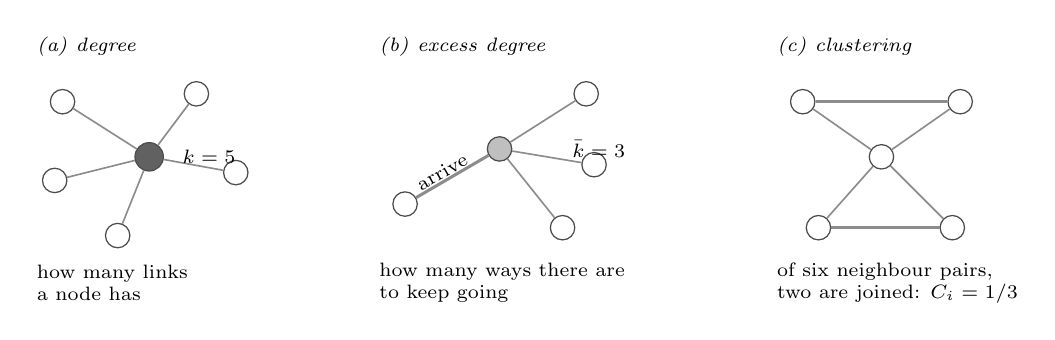
\begin{tikzpicture}
\begin{scope}
  \node[tb,anchor=west] at (-0.3,2.75) {(a) degree};
  \node[hub] (H) at (1.25,1.35) {};
  \node[nd] (h1) at (0.15,2.05) {}; \node[nd] (h2) at (0.05,1.05) {};
  \node[nd] (h3) at (0.85,0.35) {}; \node[nd] (h4) at (1.85,2.15) {};
  \node[nd] (h5) at (2.35,1.15) {};
  \draw[lnk] (H)--(h1) (H)--(h2) (H)--(h3) (H)--(h4) (H)--(h5);
  \node[lb,anchor=west] at (1.55,1.35) {$k=5$};
  \node[lb,anchor=west,align=left] at (-0.3,-0.25)
    {how many links\\ a node has};
\end{scope}
\begin{scope}[xshift=4.35cm]
  \node[tb,anchor=west] at (-0.3,2.75) {(b) excess degree};
  \node[nd] (A) at (0.15,0.75) {};
  \node[ndf] (B) at (1.35,1.45) {};
  \node[nd] (b1) at (2.45,2.15) {}; \node[nd] (b2) at (2.55,1.25) {};
  \node[nd] (b3) at (2.15,0.45) {};
  \draw[lnk,line width=1.1pt] (A)--(B);
  \draw[lnk] (B)--(b1) (B)--(b2) (B)--(b3);
  \node[lb,anchor=south,rotate=30] at (0.72,0.98) {arrive};
  \node[lb,anchor=west] at (2.15,1.45) {$\bar k=3$};
  \node[lb,anchor=west,align=left] at (-0.3,-0.25)
    {how many ways there are\\ to keep going};
\end{scope}
\begin{scope}[xshift=9.4cm]
  \node[tb,anchor=west] at (-0.3,2.75) {(c) clustering};
  \node[nd] (C) at (1.15,1.35) {};
  \node[nd] (c1) at (0.15,2.05) {}; \node[nd] (c2) at (2.15,2.05) {};
  \node[nd] (c3) at (0.35,0.45) {}; \node[nd] (c4) at (2.05,0.45) {};
  \draw[lnk] (C)--(c1) (C)--(c2) (C)--(c3) (C)--(c4);
  \draw[lnk,line width=1.1pt] (c1)--(c2) (c3)--(c4);
  \node[lb,anchor=west,align=left] at (-0.3,-0.25)
    {of six neighbour pairs,\\ two are joined: $C_i=1/3$};
\end{scope}
\end{tikzpicture}
\end{adjustbox}
\caption{\textbf{Three quantities.} (a) Degree, the number of links at a node.
(b) Excess degree: arriving along a link, the number of ways on is one less than
the degree of the node arrived at, and that degree is size-biased because
well-connected nodes are found at the ends of more links. (c) Clustering, the
fraction of a node's neighbour pairs that are themselves joined --- the
quantity every method in this chapter assumes is zero, and no real network has
zero.}
\label{fig:basics}
\end{figure}

Figure~\ref{fig:basics} fixes those three quantities, and the third of them
is the one this chapter is about.

\section{Percolation}
\label{sec:percolation-intro}
\index{percolation!on a graph}
\index{Molloy--Reed criterion|textbf}
\index{giant component}

Take a network and dilute it. Keep each link with probability $p$ and delete it
otherwise. For small $p$ what remains is a scatter of small fragments.
For large $p$ a single component contains a finite fraction of all the nodes.
Somewhere between the two the fragments merge into that giant component, and
that abrupt change is the \emph{percolation transition}.

The question is where, and the answer follows from a counting argument that the
whole book generalises.

Start at a node and follow a surviving link. It ends somewhere, and from there
the exploration continues along $\bar k$ further links, of which a fraction $p$
survive. So one surviving branch begets, on average, $p\ave{\bar k}$ further
surviving branches. If that number is less than one the exploration dies out and
components stay finite; if it is greater than one it grows without bound and a
giant component exists. The threshold is
\begin{equation}
  p_{c}\ave{\bar k}=1,
  \qquad\text{that is,}\qquad
  p_{c}=\frac{\ave{k}}{\ave{k^{2}}-\ave{k}},
  \label{eq:molloyreed}
\end{equation}
which is the Molloy--Reed criterion \citep{molloy1995}. The generating-function
apparatus behind it is due to \citet{newman2001random}. For a Poisson network,
$\ave{\bar k}=\ave{k}$ and the giant component appears at mean degree one. For a
scale-free network with $\ave{k^{2}}$ divergent, $p_{c}=0$: such networks cannot
be broken by random deletion at all.

Three features of this argument carry through to
Chapter~\ref{ch:percolation} unchanged.

First, it is a \emph{branching process}. The exploration is treated as a family
tree in which each individual has an independent number of children, and the
threshold is the point where the mean number of children reaches one. This is
exact when the network has no short loops and wrong when it does, because on a
loop the exploration comes back to somewhere it has already been and a branching
process has no way to know that.

Second, the only property of the network that entered was $\ave{\bar k}$, a
ratio of the first two moments. Everything else about $p(k)$ is irrelevant to
where the transition is. It is not irrelevant to how big the giant component is
once past it, which is the subject of Chapter~\ref{ch:giant}.

Third, deleting links at random and deleting nodes at random are the same
calculation with different bookkeeping.

\begin{calculation}{the giant component, in full}
The branching argument gives the threshold. Getting the size of the giant
component needs generating functions, which are the workhorse of
Chapter~\ref{ch:percolation} and are introduced here once.

Encode the degree distribution as a power series,
\[
  G_{0}(x)=\sum_{k}p(k)\,x^{k},
\]
so that $G_{0}(1)=1$ and $G_{0}'(1)=\ave{k}$. The corresponding function for the
excess degree --- the number of onward links from a node arrived at along a link
--- is
\[
  G_{1}(x)=\frac{G_{0}'(x)}{G_{0}'(1)},
  \qquad G_{1}'(1)=\ave{\bar k}.
\]
Let $u$ be the probability that a link, followed, leads to a finite component.
The node at the far end must have all of \emph{its} onward links lead to finite
components, and each does so either because it was deleted (probability $1-p$)
or because it was kept and led to a finite component (probability $pu$). Summing
over the number of onward links,
\[
  u=G_{1}\bigl(1-p+pu\bigr).
\]
The fraction of nodes \emph{not} in the giant component is the same statement
made at a node rather than along a link, so the giant component fraction is
\[
  S=1-G_{0}\bigl(1-p+pu\bigr).
\]
The trivial solution $u=1$ always exists and gives $S=0$. It becomes unstable
when the derivative of the right-hand side at $u=1$ exceeds one, that is when
$p\,G_{1}'(1)>1$ --- Eq.~\eqref{eq:molloyreed} again. Threshold and order
parameter are the linearisation and the full solution of one equation, which is
the observation Chapter~\ref{ch:giant} is built on.
\end{calculation}

\begin{figure}[t]
\centering
\begin{adjustbox}{max width=0.95\linewidth}
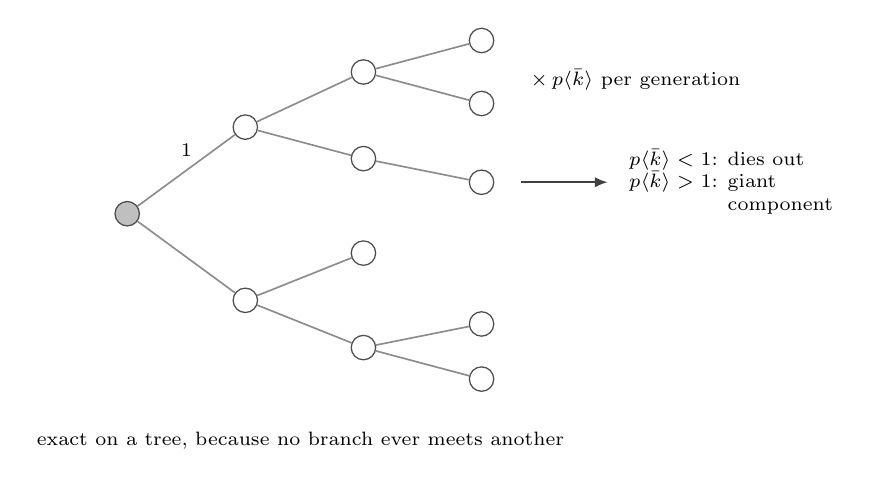
\begin{tikzpicture}
% ---- branching picture
\node[ndf] (r) at (0,0) {};
\node[nd] (a1) at (1.5,1.1) {}; \node[nd] (a2) at (1.5,-1.1) {};
\node[nd] (b1) at (3.0,1.8) {}; \node[nd] (b2) at (3.0,0.7) {};
\node[nd] (b3) at (3.0,-0.5) {}; \node[nd] (b4) at (3.0,-1.7) {};
\node[nd] (c1) at (4.5,2.2) {}; \node[nd] (c2) at (4.5,1.4) {};
\node[nd] (c3) at (4.5,0.4) {}; \node[nd] (c4) at (4.5,-1.4) {};
\node[nd] (c5) at (4.5,-2.1) {};
\draw[lnk] (r)--(a1) (r)--(a2);
\draw[lnk] (a1)--(b1) (a1)--(b2) (a2)--(b3) (a2)--(b4);
\draw[lnk] (b1)--(c1) (b1)--(c2) (b2)--(c3) (b4)--(c4) (b4)--(c5);
\node[lb,anchor=south] at (0.75,0.60) {$1$};
\node[lb,anchor=west] at (5.0,1.7)
  {$\times\,p\ave{\bar k}$ per generation};
\draw[msg] (5.0,0.4) -- (6.1,0.4);
\node[lb,anchor=west,align=left] at (6.25,0.4)
  {$p\ave{\bar k}<1$: dies out\\
   $p\ave{\bar k}>1$: giant\\ \phantom{$p\ave{\bar k}>1$: }component};
\node[lb,anchor=north,align=center] at (2.2,-2.65)
  {exact on a tree, because no branch ever meets another};
\end{tikzpicture}
\end{adjustbox}
\caption{\textbf{Percolation as a branching process.} Following a surviving link
leads to a node with $\bar k$ further links, a fraction $p$ of which survive, so
each branch begets $p\ave{\bar k}$ branches. The transition is where that number
passes one. Every threshold in this book is a version of this statement; what
changes from chapter to chapter is what a branch is and what it carries.}
\label{fig:branching}
\end{figure}

Figure~\ref{fig:branching} is that argument drawn: one branch begetting more
than one branch, and why it is exact on a tree.

\section{Models on networks}
\label{sec:models}

Percolation asks about the network itself. The rest of the book puts something
\emph{on} the network --- a variable at every node, and an energy that says which
combinations of variables are cheap. Three of the models that run through the book are introduced here, and all
three appear now on the same small graph, so the family resemblance is
visible. For the wider map --- spin models, $k$-core percolation, epidemic
thresholds and the rest, on equilibrium and growing networks alike ---
\citet{dorogovtsev2008} is the review to read alongside this chapter, which
takes only what the later chapters use.

\subsection{Ising model}
\label{sec:ising-intro}
\index{Ising model|textbf}

Put a variable $\sigma_{i}=\pm1$ on every node --- historically a magnetic
moment pointing up or down --- and let neighbouring nodes prefer to agree:
\begin{equation}
  \mathcal{H}=-J\sum_{\langle ij\rangle}\sigma_{i}\sigma_{j}
              -B\sum_{i}\sigma_{i},
  \label{eq:ising-intro}
\end{equation}
the first sum over links, the second over nodes, $J>0$ the strength of the
preference and $B$ an external field pushing every spin one way. Configurations
occur with the Boltzmann probability $\propto e^{-\beta\mathcal{H}}$, where
$\beta=1/T$ is the inverse temperature.

The behaviour is a competition. At high temperature the spins are essentially
independent and the average magnetisation $m=\ave{\sigma}$ is zero. At low
temperature agreement wins, a majority forms, and $m\ne0$ even with $B=0$. In
between is a critical temperature $T_{c}$.

On a treelike network the answer is a one-line calculation, and it is
\emph{the same line as percolation}. Write $t=\tanh\beta J$ for the strength
with which one spin transmits its bias to a neighbour. Then
\begin{equation}
  t\,\ave{\bar k}=1
  \label{eq:tc-intro}
\end{equation}
locates $T_{c}$. Compare Eq.~\eqref{eq:molloyreed}: the occupation probability
$p$ has been replaced by $\tanh\beta J$ and nothing else has changed. A
correlation propagating through the network and a cluster spreading through it
are the same branching process counted with a different weight.
Chapter~\ref{ch:potts} shows that the two are the same model at two values of
one parameter.

Equation~\eqref{eq:tc-intro} is exact on a random graph with any degree
distribution, and the same replica calculation returns the critical exponents
from the moments of $p(k)$ \citep{leone2002}. The parallel with percolation
survives into the pathologies: where $\ave{k^{2}}$ diverges $\ave{\bar k}$ is
infinite, Eq.~\eqref{eq:tc-intro} has no finite root and the system is ordered
at every temperature, which is the counterpart of $p_{c}=0$ above; where
$\ave{k^{2}}$ is finite but $\ave{k^{4}}$ is not, $T_{c}$ is finite and the
exponents are not the mean-field ones.

\subsection{Vertex covering}
\label{sec:cover-intro}
\index{vertex cover|textbf}
\index{NP-hardness}

The second model has no temperature in it at all. A \emph{vertex cover} of a graph
is a set of nodes such that every link has at least one endpoint in the set ---
guards posted at corridor junctions so that every corridor is watched. Covering
everything is easy; covering everything with as few nodes as possible is the
\emph{minimum vertex cover} problem, and it is NP-hard \citep{karp1972}: no
algorithm is known that solves it in time polynomial in the size of the graph,
and it is widely believed none exists.

Statistical physics gets a grip on it by making it a model. Put
$x_{i}\in\{0,1\}$ on every node, $1$ meaning covered, and write
\begin{equation}
  \mathcal{H}=\sum_{i}x_{i},
  \qquad\text{subject to}\quad
  x_{i}+x_{j}\ge1 \ \ \text{on every link}.
  \label{eq:vc-intro}
\end{equation}
The energy is just the number of guards, the constraint is hard --- infinitely
costly to violate --- and the minimum vertex cover is the ground state. Asking
for the ground state of a disordered system is asking an optimisation question,
and the whole apparatus of statistical mechanics becomes available for it. This
was the move that opened the subject \citep{weigt2000}.

One fact about vertex cover will matter repeatedly. Consider a node of degree
one --- a \emph{leaf}. Its single link must be covered, and covering it at the
leaf can never be better than covering it at the neighbour, since the neighbour
may cover other links too. So there is always a minimum cover that takes the
neighbour and not the leaf, and one can simply remove both, together with every
link the neighbour touched, and repeat. This is \emph{leaf removal}
\citep{bauer2001}. When it consumes the whole graph it has found a minimum cover
and \emph{proved} it minimum. When it stalls, what is left is called the
\emph{core}, and it is the hard part.

For a Poisson random graph, leaf removal succeeds when the mean degree is below
$e=2.718\ldots$ and stalls above it \citep{bauer2001,weigt2000}. That number
will reappear, from a completely different direction, in
Chapter~\ref{ch:hittingset}.

\subsection{Hitting set}
\label{sec:hs-intro}
\index{hitting set problem|textbf}

Vertex cover generalises in the obvious direction. Instead of links --- sets of
two nodes --- take a family of sets of any size, and ask for the smallest
collection of elements meeting every one of them. That is the \emph{hitting set}
problem \citep{mezard2007}, and vertex cover is the special case in which every
set has two members.

The Hamiltonian is Eq.~\eqref{eq:vc-intro} with the constraint read over
hyperedges rather than links, $\sum_{i\in a}x_{i}\ge1$ for every set $a$.
Nothing about the formulation changes; what changes is that the constraint now
couples three, four or ten variables at once, and Chapter~\ref{ch:hittingset}
shows that a limit everybody takes for granted on graphs stops being correct the
moment it does.

This pairing --- vertex cover as the two-element case of hitting set --- is the
reason Chapters~\ref{ch:hittingset} and~\ref{ch:cover} are adjacent. They are one
problem.

\begin{figure}[t]
\centering
\begin{adjustbox}{max width=\linewidth}
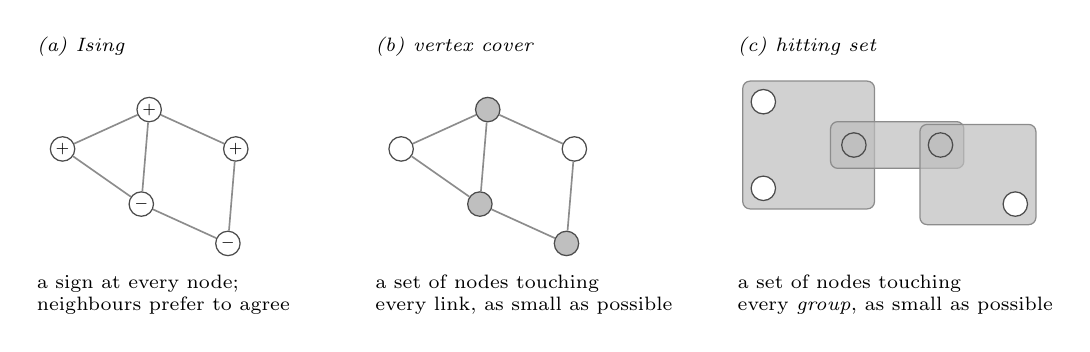
\begin{tikzpicture}
\def\gA{\node[nd] (v1) at (0.15,1.55) {}; \node[nd] (v2) at (1.25,2.05) {};
        \node[nd] (v3) at (1.15,0.85) {}; \node[nd] (v4) at (2.35,1.55) {};
        \node[nd] (v5) at (2.25,0.35) {};}
% ---- Ising
\begin{scope}
  \node[tb,anchor=west] at (-0.3,2.85) {(a) Ising};
  \node[nd] (a1) at (0.15,1.55) {\tiny$+$}; \node[nd] (a2) at (1.25,2.05) {\tiny$+$};
  \node[nd] (a3) at (1.15,0.85) {\tiny$-$}; \node[nd] (a4) at (2.35,1.55) {\tiny$+$};
  \node[nd] (a5) at (2.25,0.35) {\tiny$-$};
  \draw[lnk] (a1)--(a2) (a1)--(a3) (a2)--(a3) (a2)--(a4) (a3)--(a5) (a4)--(a5);
  \node[lb,anchor=west,align=left] at (-0.3,-0.30)
    {a sign at every node;\\ neighbours prefer to agree};
\end{scope}
% ---- vertex cover
\begin{scope}[xshift=4.3cm]
  \node[tb,anchor=west] at (-0.3,2.85) {(b) vertex cover};
  \node[nd]  (b1) at (0.15,1.55) {}; \node[ndf] (b2) at (1.25,2.05) {};
  \node[ndf] (b3) at (1.15,0.85) {}; \node[nd]  (b4) at (2.35,1.55) {};
  \node[ndf] (b5) at (2.25,0.35) {};
  \draw[lnk] (b1)--(b2) (b1)--(b3) (b2)--(b3) (b2)--(b4) (b3)--(b5) (b4)--(b5);
  \node[lb,anchor=west,align=left] at (-0.3,-0.30)
    {a set of nodes touching\\ every link, as small as possible};
\end{scope}
% ---- hitting set
\begin{scope}[xshift=8.9cm]
  \node[tb,anchor=west] at (-0.3,2.85) {(c) hitting set};
  \node[nd]  (c1) at (0.15,2.15) {}; \node[nd]  (c2) at (0.15,1.05) {};
  \node[ndf] (c3) at (1.30,1.60) {}; \node[ndf] (c4) at (2.40,1.60) {};
  \node[nd]  (c5) at (3.35,0.85) {};
  \begin{scope}[on background layer]
    \node[cx,fill=black!26,fill opacity=0.7,fit=(c1)(c2)(c3)]{};
    \node[cx,fill=black!26,fill opacity=0.7,inner sep=3.8pt,fit=(c3)(c4)]{};
    \node[cx,fill=black!26,fill opacity=0.7,fit=(c4)(c5)]{};
  \end{scope}
  \node[lb,anchor=west,align=left] at (-0.3,-0.30)
    {a set of nodes touching\\ every \emph{group}, as small as possible};
\end{scope}
\end{tikzpicture}
\end{adjustbox}
\caption{\textbf{Three models, one graph.} (a) The Ising model decorates the
nodes with signs and pays for disagreement across links. (b) Vertex cover picks
a set of nodes (filled) meeting every link. (c) Hitting set is the same question
with links replaced by groups of any size --- and the groups, drawn here as
boxes, are already the complexes of Chapter~\ref{ch:chygraphs}. What the three
share is a variable per node, an energy, and a question about the resulting
Boltzmann measure; what they differ in is what the message of
Sec.~\ref{sec:cavity} has to carry.}
\label{fig:threemodels}
\end{figure}

Figure~\ref{fig:threemodels} puts the three side by side on one graph: they
differ in what decorates the nodes and what is paid for, not in the object
underneath.

\subsection{What these have in common}

All three are a variable at every node, an energy summing local terms, and a
Boltzmann measure $\propto e^{-\beta\mathcal{H}}$. Optimisation is the
zero-temperature limit of that measure: as $\beta\to\infty$ all the weight
concentrates on the lowest-energy configurations, so ``find the minimum vertex
cover'' and ``take $T\to0$ in this model'' are the same instruction. The
apparatus does not distinguish them, which is why one method can serve a
magnet and an NP-hard optimisation problem.

One caveat about that limit runs through the book. Taking
$T\to0$ inside an approximation is not the same as taking it in the exact
answer, and Chapter~\ref{ch:hittingset} exhibits a case, simple enough to check
by hand, where the standard zero-temperature treatment gives $1/2$ and the truth
is $1/3$.

\section{Mean field}
\label{sec:meanfield}
\index{mean-field theory|textbf}

The oldest way to solve a model like Eq.~\eqref{eq:ising-intro} is to assume
each spin feels not its neighbours but their average. Replace
$\sigma_{j}\to m$ for every neighbour, and a node of degree $k$ then sits in an
effective field $Jkm$, giving the self-consistency condition
\begin{equation}
  m=\tanh\bigl(\beta J\ave{k}m\bigr).
  \label{eq:mf}
\end{equation}
For small $m$ the right-hand side is $\beta J\ave{k}m$, so a non-zero solution
appears when $\beta J\ave{k}=1$.

This is wrong. Compare it with Eq.~\eqref{eq:tc-intro}: mean field gives $\beta J\ave{k}=1$ where the correct
treelike answer is $\tanh(\beta J)\ave{\bar k}=1$. Two errors, in opposite
directions. Mean field uses $\ave{k}$ where it should use the excess degree
$\ave{\bar k}$ --- it forgets that the walk arrived along a link and cannot
leave by it --- and it uses $\beta J$ where it should use $\tanh\beta J$,
because it treats the neighbour's spin as a fixed number rather than a
fluctuating variable that only partially transmits.

Mean field becomes exact when every node has many neighbours, since then the sum
of many weakly correlated influences really is close to its average. In infinite
dimension, or on a fully connected graph, it is right. On a sparse network,
where a node has three or five neighbours and each one matters individually, it
is not, and the fix is the subject of the next section.

What survives from mean field is the \emph{style} of answer: a self-consistency
condition for one number, solved by looking for where a non-trivial solution
appears. Everything in this book has that shape. What changes is that the one
number becomes a message, and then a distribution of messages.

\section{The cavity method}
\label{sec:cavity}
\index{cavity method|textbf}
\index{belief propagation|textbf}
\index{Bethe--Peierls approximation|textbf}
\index{message passing}

Our core idea is geometric before it is a calculation.

Take a node $i$ and remove it, leaving a hole --- a \emph{cavity}. On a tree,
removing $i$ disconnects its neighbours from one another completely: the
branches that hung off $i$ are now separate networks with no path between them.
Whatever is going on in one branch is therefore independent of whatever is going
on in another. That independence is the trick, and it converts a problem
in which every variable is coupled to every other into a problem about one
branch at a time.

Concretely, let each neighbour $j$ of $i$ send $i$ a summary of what its branch
would do if $i$ were absent. Call that summary a \emph{message}. For the Ising
model the message is a field $h_{j\to i}$: the effective bias that branch $j$
exerts on node $i$. Because the branches are independent, the total bias on $i$
is just the sum of the messages arriving at it, and the message $i$ sends onward
to some other neighbour $l$ is built from the messages $i$ receives from
everyone except $l$:
\begin{equation}
  h_{i\to l}=B+\sum_{j\in\partial i\setminus l}
             u\bigl(h_{j\to i}\bigr),
  \label{eq:cavity-intro}
\end{equation}
where $\partial i$ is the set of neighbours of $i$ and $u(\cdot)$ is the
function that says how much of a bias survives one link. This is the
\emph{cavity recursion}. Under other names it is the Bethe--Peierls
approximation \citep{bethe1935} and \emph{belief propagation}
\citep{yedidia2005}; they are the same equations arrived at by physicists,
statisticians and computer scientists independently; \citet{mezard2009} set the
three vocabularies side by side.

\begin{figure}[t]
\centering
\begin{adjustbox}{max width=0.95\linewidth}
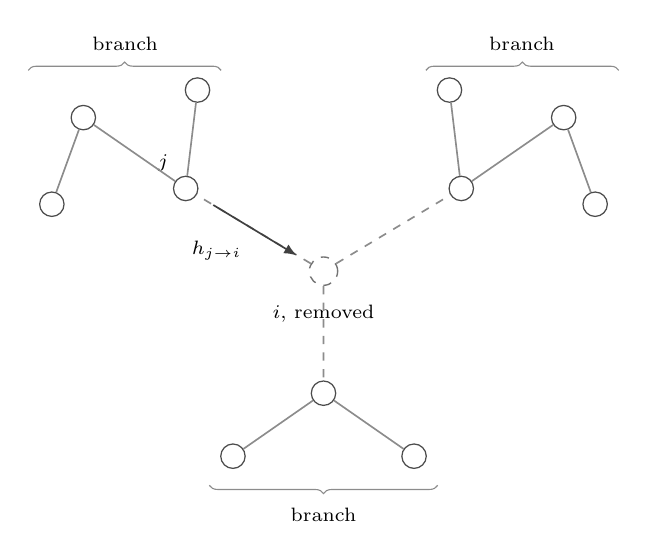
\begin{tikzpicture}
% node i, removed: drawn as a dashed outline so the hole it leaves is visible
\node[circle,draw=black!55,dashed,fill=white,minimum size=3.6mm,inner sep=0pt,
      line width=.5pt] (i) at (0,0) {};
\node[lb,anchor=north] at (0,-0.30) {$i$, removed};
% its three neighbours, and the branch hanging off each
\node[nd] (j1) at (-1.75,1.05) {}; \node[nd] (j2) at (1.75,1.05) {};
\node[nd] (j3) at (0,-1.55) {};
\node[lb,anchor=south east] at (-1.85,1.15) {$j$};
\draw[lnk,dashed] (i)--(j1) (i)--(j2) (i)--(j3);
\node[nd] (p1) at (-3.05,1.95) {}; \node[nd] (p2) at (-1.60,2.30) {};
\node[nd] (p3) at (-3.45,0.85) {};
\draw[lnk] (j1)--(p1) (j1)--(p2) (p1)--(p3);
\node[nd] (q1) at (3.05,1.95) {}; \node[nd] (q2) at (1.60,2.30) {};
\node[nd] (q3) at (3.45,0.85) {};
\draw[lnk] (j2)--(q1) (j2)--(q2) (q1)--(q3);
\node[nd] (r1) at (-1.15,-2.35) {}; \node[nd] (r2) at (1.15,-2.35) {};
\draw[lnk] (j3)--(r1) (j3)--(r2);
% the message, with the label set clear of the arrow
\draw[msg] (-1.40,0.84) -- (-0.34,0.20);
\node[lb,anchor=east] at (-0.92,0.26) {$h_{j\to i}$};
% the three branches, named
\draw[decorate,decoration={brace,amplitude=3pt},black!45]
  (-3.75,2.55) -- (-1.30,2.55);
\node[lb,anchor=south] at (-2.52,2.68) {branch};
\draw[decorate,decoration={brace,amplitude=3pt},black!45]
  (1.30,2.55) -- (3.75,2.55);
\node[lb,anchor=south] at (2.52,2.68) {branch};
\draw[decorate,decoration={brace,amplitude=3pt,mirror},black!45]
  (-1.45,-2.72) -- (1.45,-2.72);
\node[lb,anchor=north] at (0,-2.88) {branch};
\end{tikzpicture}
\end{adjustbox}
\caption{\textbf{The cavity.} Removing node $i$ from a tree separates its
branches completely. Each branch then summarises itself in a single message
$h_{j\to i}$, and because the branches are independent those messages simply
add. Equation~\eqref{eq:cavity-intro} is that statement written down. Everything
in Chapters~\ref{ch:statmech} to~\ref{ch:satisfiability} is this picture with a
complex in place of a node, and the only question that ever changes is what the
message carries.}
\label{fig:cavity}
\end{figure}

Figure~\ref{fig:cavity} is the construction, and the whole of the method is in
it: remove a node, and what is left summarises itself.

Two ways of using Eq.~\eqref{eq:cavity-intro} run side by side throughout the
book and should not be confused.

\emph{On one instance}, one has an actual graph, initialises the messages
arbitrarily, and iterates until they stop changing. That is belief propagation,
it is an algorithm, and it returns an answer for that particular graph.

\emph{On an ensemble}, one gives up on individual messages and asks for their
\emph{distribution} over a random graph. Equation~\eqref{eq:cavity-intro} then
becomes an equation for a probability distribution $P(h)$, self-consistent in
the sense that a message built out of $\bar k$ messages drawn from $P$ is itself
drawn from $P$. This gives the typical behaviour of the whole class of graphs at
once, and it is what all the thresholds in this book are.

\begin{calculation}{the cavity recursion for the Ising model, and its threshold}
For Eq.~\eqref{eq:ising-intro} the message function is
\[
  u(h)=\frac{1}{\beta}\,\mathrm{atanh}
       \bigl[\tanh(\beta J)\tanh(\beta h)\bigr],
\]
which is derived by summing over the single spin $\sigma_{j}$ at the far end of
the link: a spin biased by $h$ transmits a bias reduced by the factor
$t=\tanh\beta J$, and the composition of two hyperbolic tangents is what
enforces that the transmitted bias can never exceed the link's own strength.

Set $B=0$ and ask when the paramagnetic solution $h\equiv0$ becomes unstable.
For small $h$,
\[
  u(h)\simeq t\,h,
\]
so Eq.~\eqref{eq:cavity-intro} linearises to
$h_{i\to l}=t\sum_{j\in\partial i\setminus l}h_{j\to i}$: a small bias is
multiplied by $t$ at every step and fans out over $\bar k$ branches. Averaging
over the ensemble, a perturbation grows when
\[
  t\,\ave{\bar k}>1,
\]
which is Eq.~\eqref{eq:tc-intro}. For a $c$-regular graph $\ave{\bar k}=c-1$ and
this is the classical Bethe-lattice result $\tanh\beta J_{c}=1/(c-1)$.

Three features of this calculation are what Chapter~\ref{ch:statmech}
generalises. The message is a \emph{number} here
only because the interaction is on a single link; when the interaction lives
inside a group, the message becomes a distribution. The factor $t$ came from
summing over the interior of one link \emph{exactly}; when the interior is
larger, that sum is larger but still exact. And the counting $\ave{\bar k}$ is
independent of both --- it is a property of the network, not of the model.
Separating those three is what lets one calculation serve every model in this
book.
\end{calculation}

\section{Replica symmetry and symmetry breaking}
\label{sec:replicas}
\index{replica symmetry breaking|textbf}
\index{de Almeida--Thouless line}

The cavity method as just described contains an assumption that is easy to miss.
In writing a single distribution $P(h)$ and asking it to be self-consistent, one
has assumed that the system has essentially \emph{one} state --- that two runs
of the model would look statistically alike. This is
\emph{replica symmetry}, so called because in the older replica formalism
\citep{mezard1987} it appears as a symmetry among $n$ copies of the system.

For the Ising model at high temperature it is true. For an Ising model with
random signs of $J$, a spin glass, it is false below a certain temperature: the
energy landscape breaks into exponentially many valleys separated by barriers,
each valley a perfectly good ``state'', and no single $P(h)$ describes them all.
The same happens in hard optimisation problems --- for vertex cover on a Poisson
graph it happens at mean degree $e$, the point where leaf removal stalls
\citep{weigt2000,bauer2001}; Chapter~\ref{ch:cover} shows that the two are one
point.

The remedy is \emph{one-step replica symmetry breaking}: a distribution over
valleys, and within each valley a distribution over messages --- a distribution
of distributions \citep{mezard2001}. This book does that calculation twice, in
Secs.~\ref{sec:colouring-sp} and~\ref{sec:sat-sp}, and only where the messages
are warnings and the distribution is over a finite alphabet; everywhere else it
does not. So it needs to know when the calculation it \emph{does} do has
stopped being right, and there are three reliable signals.

\emph{The stability of the symmetric solution.} Perturb the messages and ask
whether the perturbation grows. For the Ising model the relevant condition turns
out to be $t^{2}\ave{\bar k}=1$ rather than $t\ave{\bar k}=1$ --- the
\emph{de Almeida--Thouless line} \citep{dealmeida1978} --- because a perturbation
of \emph{random sign} is transmitted with $t$ and its effect measured by
squaring. That squaring is the difference between the ferromagnetic
transition and the spin-glass one, and Chapter~\ref{ch:ising} obtains both from
the same expression by squaring one factor.

\emph{Negative entropy.} A replica-symmetric calculation of a discrete problem
returns the logarithm of a number of configurations. Where that goes negative
the calculation is counting fewer than one configuration, which is impossible,
and the answer it gives is an underestimate.

\emph{The iteration stops converging.} Run the equations and they cycle or
wander. This is the practical signal and it is the one that usually arrives
first.

None of these gives the right answer. All of them show that the answer in hand
is wrong. This book flags every place they fire.

\section{The tree assumption, and why real networks break it}
\label{sec:treebreaks}
\index{tree assumption|textbf}
\index{treelike}
\index{clustering!and the tree assumption}

In this section we collect the tree assumption made by every method above and
measure how badly real networks violate it, since that violation is what the
rest of the book is written to repair.

The percolation threshold came from a
branching process, which is exact when no branch ever meets another. The cavity
recursion came from removing a node and finding its branches independent, which
is true when the branches are not joined behind its back. Both statements are
the same statement: \textbf{the network must be locally treelike}. Follow links
away from a node must not lead back to it.

Real networks come back. The clustering coefficient of
Eq.~\eqref{eq:clustering} measures exactly how often, and it is not small: in
the ten networks of Table~\ref{tab:real} it runs from $0.006$ to $0.65$. A
triangle is a loop of length three, the shortest possible, and every triangle is
a place where two branches that the theory believes to be independent are in
fact the same branch.

\begin{figure}[t]
\centering
\begin{adjustbox}{max width=0.95\linewidth}
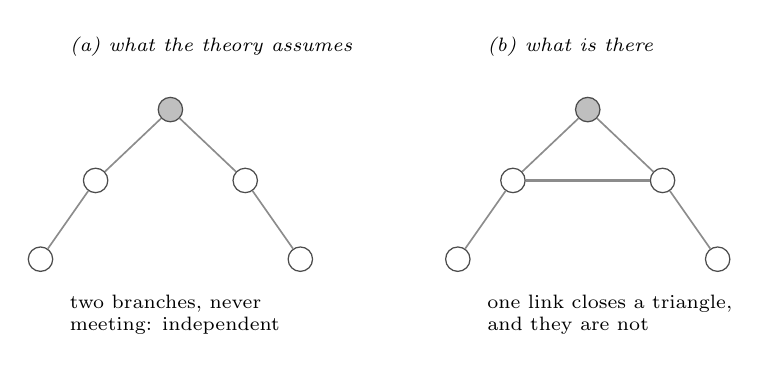
\begin{tikzpicture}
\begin{scope}
  \node[tb,anchor=west] at (-0.3,2.35) {(a) what the theory assumes};
  \node[ndf] (i) at (1.1,1.55) {};
  \node[nd] (j) at (0.15,0.65) {}; \node[nd] (l) at (2.05,0.65) {};
  \node[nd] (j1) at (-0.55,-0.35) {}; \node[nd] (l1) at (2.75,-0.35) {};
  \draw[lnk] (i)--(j) (i)--(l) (j)--(j1) (l)--(l1);
  \node[lb,anchor=west,align=left] at (-0.3,-1.05)
    {two branches, never\\ meeting: independent};
\end{scope}
\begin{scope}[xshift=5.3cm]
  \node[tb,anchor=west] at (-0.3,2.35) {(b) what is there};
  \node[ndf] (I) at (1.1,1.55) {};
  \node[nd] (J) at (0.15,0.65) {}; \node[nd] (L) at (2.05,0.65) {};
  \node[nd] (J1) at (-0.55,-0.35) {}; \node[nd] (L1) at (2.75,-0.35) {};
  \draw[lnk] (I)--(J) (I)--(L) (J)--(J1) (L)--(L1);
  \draw[lnk,line width=1.2pt] (J)--(L);
  \node[lb,anchor=west,align=left] at (-0.3,-1.05)
    {one link closes a triangle,\\ and they are not};
\end{scope}
\end{tikzpicture}
\end{adjustbox}
\caption{\textbf{The assumption, and the world.} The cavity recursion adds the
messages arriving at a node because the branches sending them cannot influence
one another. One extra link --- the heavy one --- makes that false, and there is
no repair within the graph: the two messages are now correlated in a way a sum
cannot express. Chapter~\ref{ch:chygraphs} does not repair it either. It stops
treating the triangle as three links.}
\label{fig:treebreaks}
\end{figure}

Figure~\ref{fig:treebreaks} draws the gap between the two.

How much does this matter? Two answers, and they are of different kinds.

\paragraph{Quantitatively, it is a wrong number.} Take a network with two
triangles at every node and compare it with a $4$-regular network --- same
degree everywhere, same $\ave{\bar k}$, so Eq.~\eqref{eq:tc-intro} gives them the
same critical temperature. It is wrong by $13.9$ per cent, and
Chapter~\ref{ch:ising} computes the correct value in closed form and confirms it
by Monte Carlo at $14.2$ per cent. The sign is not the one most people guess:
clustering \emph{lowers} $T_{c}$.

\paragraph{Qualitatively, it is the wrong phase.} Hyperbolic random graphs, which
are clustered because of the geometry they are built in, retain an extensive
leaf-removal core at \emph{every} mean degree, with no transition at all. Their
degree-matched configuration model --- the same $p(k)$, the same $\ave{\bar k}$,
the same assortativity to within a few per cent --- has no core whatever until
the mean degree reaches somewhere between $4.5$ and $10$. The two graphs agree
on every quantity the theory of this chapter can see, and they are in different
phases. Whatever separates them lies outside $p(k)$ by construction, and it is
clustering.

The second example rules out the obvious response. One cannot rescue the situation by measuring the degree distribution
more carefully, or by correlating the degrees of adjacent nodes
\citep{vazquez2003vw}, or by any refinement of a description whose atoms are
nodes and links. The
information that distinguishes the two graphs is not in that description at all.

So the field has had, for twenty-five years, a method that works and a
systematic reason why it should not apply to the objects it is applied to.

\section{Generalised belief propagation}
\label{sec:gbp-intro}
\index{generalised belief propagation}
\index{Kikuchi approximation}
\index{cluster variation method}
\index{region graph}

There is an established answer to loops, and it is worth stating here because
this book uses it later and because it is the alternative to the route the rest
of the book takes.

Belief propagation is exact on a tree because a tree decomposes into nodes and
links with every variable, and every interaction, counted exactly once. When the
network is not a tree that bookkeeping fails. The remedy, due to Kikuchi and
given its message-passing form by \citet{yedidia2005}, is to keep the
bookkeeping and enlarge the units: work with \emph{regions} --- sets of
variables treated as single objects --- and close the family of regions under
intersection. Each region $R$ is assigned a counting number fixed by
M\"obius inversion,
\begin{equation}
  c_{R}=1-\sum_{R'\supsetneq R}c_{R'},
  \label{eq:mobius-intro}
\end{equation}
which is precisely the condition that every variable and every interaction is
counted once across the whole family. Messages then pass from each region to its
sub-regions rather than from node to node.

Three properties matter for what follows. The scheme \emph{contains} the
cavity method: when the regions are the interactions and the single variables,
Eq.~\eqref{eq:mobius-intro} returns $c_{v}=1-k$ and the update reduces to
Eq.~\eqref{eq:cavity-intro}. It is \emph{exact} whenever the closed family of
regions forms a junction tree, which is the loop-free condition one level up. And
it costs $2^{|R|}$ per region, so it buys accuracy with enumeration, and the
purchase stops being affordable when the regions grow.

What it does not give is an ensemble. The regions are an explicit list drawn
from one network, and the messages are functions on them, where everything else
in this chapter carries a distribution over a random graph.
Chapter~\ref{ch:gbp} measures what this method recovers, and what it costs, on
three classes of network.

The next chapter's response is not to patch the method. It is to change what the
method is applied to: if a triangle is a problem when treated as three links,
stop treating it as three links.



% sources
% - Bethe-Peierls background: Vazquez & Weigt, Phys. Rev. E 67, 027101 (2003)
% - textbook background: Mezard & Montanari; Newman
% - the closing section (why real networks break treelikeness) motivates the book

\chapter{Chygraphs}
\label{ch:chygraphs}

\section{A paper is not a set of links}
\label{sec:paper}

In this chapter we define the chygraph and show what it represents that a graph
or a hypergraph cannot. We motivate it with the scientific literature, which
has been mapped many times over, whose maps disagree with one another, and
where the reason they disagree is exactly the subject of the chapter.

The system itself is simple. A paper is written by some authors. It cites
some other papers. Those papers were written by their own authors and cited
their own predecessors. That is the whole system --- documents, the people who
wrote them, and the pointers between documents --- and it has been drawn as a
network in at least four different ways \citep{newman2001,barabasi2002}.

The \emph{citation network} keeps the papers and the pointers: a node is a
paper, a directed link is a citation \citep{redner1998}. It is the right object
if the question is how knowledge flows, and it has nothing to say about who
wrote anything. The \emph{co-authorship network} keeps the people: a node is an
author, and two authors are linked if they have written a paper together. It is
the right object if the question is who works with whom, and it has nothing to
say about citation. The \emph{bipartite author--paper graph} keeps both kinds of
thing, authors and papers, with a link wherever a person wrote a document; it
loses the citations again. And the \emph{author hypergraph} replaces the
co-authorship links by hyperedges, one per paper, so that a five-author paper is
one object rather than ten pairwise links \citep{vasilyeva2021}.

Four maps, four different objects, and each of them made by throwing away
something that was in the system to begin with (Fig.~\ref{fig:projections}).
They also throw away different things, so a result proved on one of them
cannot be quoted on another. That is what happens when a system whose parts
contain other parts is forced into a language
whose only relation is ``these two things are joined.''

\begin{figure}[t]
\centering
\begin{adjustbox}{max width=\linewidth}
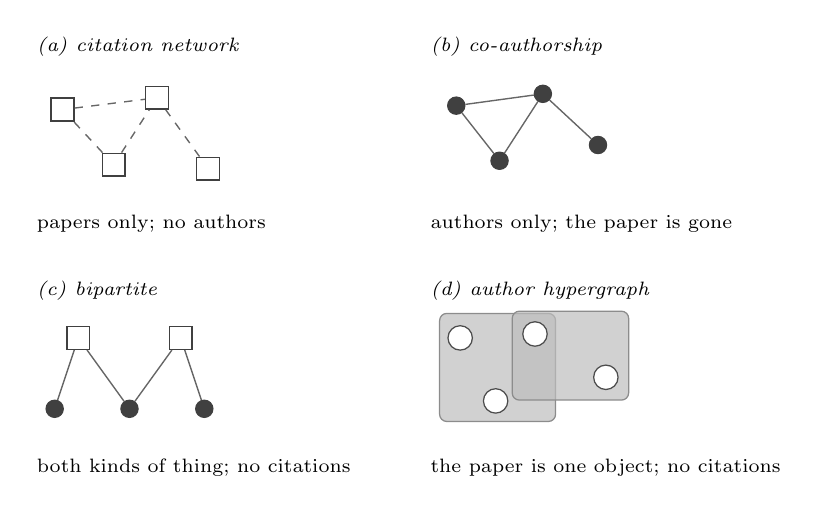
\begin{tikzpicture}
% ---- (a) citation network
\begin{scope}
  \node[tb,anchor=west] at (-0.1,2.15) {(a) citation network};
  \node[cpx] (p1) at (0.35,1.35) {}; \node[cpx] (p2) at (1.55,1.50) {};
  \node[cpx] (p3) at (1.00,0.65) {}; \node[cpx] (p4) at (2.20,0.60) {};
  \draw[incd] (p1)--(p2) (p3)--(p1) (p3)--(p2) (p4)--(p2);
  \node[lb,anchor=west,align=left] at (-0.1,-0.10) {papers only; no authors};
\end{scope}
% ---- (b) co-authorship
\begin{scope}[xshift=5.0cm]
  \node[tb,anchor=west] at (-0.1,2.15) {(b) co-authorship};
  \node[atm] (a1) at (0.35,1.40) {}; \node[atm] (a2) at (1.45,1.55) {};
  \node[atm] (a3) at (0.90,0.70) {}; \node[atm] (a4) at (2.15,0.90) {};
  \draw[inc] (a1)--(a2)--(a3)--(a1) (a2)--(a4);
  \node[lb,anchor=west,align=left] at (-0.1,-0.10) {authors only; the paper is gone};
\end{scope}
% ---- (c) bipartite
\begin{scope}[yshift=-3.1cm]
  \node[tb,anchor=west] at (-0.1,2.15) {(c) bipartite};
  \node[cpx] (q1) at (0.55,1.55) {}; \node[cpx] (q2) at (1.85,1.55) {};
  \node[atm] (b1) at (0.25,0.65) {}; \node[atm] (b2) at (1.20,0.65) {};
  \node[atm] (b3) at (2.15,0.65) {};
  \draw[inc] (q1)--(b1) (q1)--(b2) (q2)--(b2) (q2)--(b3);
  \node[lb,anchor=west,align=left] at (-0.1,-0.10) {both kinds of thing; no citations};
\end{scope}
% ---- (d) author hypergraph
\begin{scope}[xshift=5.0cm,yshift=-3.1cm]
  \node[tb,anchor=west] at (-0.1,2.15) {(d) author hypergraph};
  \node[nd] (c1) at (0.40,1.55) {}; \node[nd] (c2) at (1.35,1.60) {};
  \node[nd] (c3) at (0.85,0.75) {}; \node[nd] (c4) at (2.25,1.05) {};
  \begin{scope}[on background layer]
    \node[cx,fill=black!26,fill opacity=0.7,fit=(c1)(c2)(c3)]{};
    \node[cx,fill=black!26,fill opacity=0.7,inner sep=3.6pt,fit=(c2)(c4)]{};
  \end{scope}
  \node[lb,anchor=west,align=left] at (-0.1,-0.10) {the paper is one object; no citations};
\end{scope}
\end{tikzpicture}
\end{adjustbox}
\caption{\textbf{Four maps of one system.} The scientific literature drawn four
ways. Filled circles are authors, rectangles and shaded boxes are papers, solid
lines are authorship and dashed lines citation. Each map is made by discarding
something that was in the system: (a) forgets who wrote anything, (b) and (d)
forget citation, and (b) also forgets that a paper with five authors is one act
and not ten. No two of them are the same object, so nothing proved on one can be
quoted on another. Where two complexes overlap, as in (d), the shading
compounds, so a darker patch marks the atoms they share --- a convention used
throughout the book.}
\label{fig:projections}
\end{figure}

A single paper is neither a node nor a link. It is a small structured thing in its own right: it has an author list,
and it has a reference list. The author list is a set of people. The reference
list is a set of \emph{other papers}. And the two lists do not mix --- no author
appears in the bibliography as a reference, and no reference is a co-author.

Suppose we agree to call the paper one object and its two lists the internal structure of that object.
Then the paper's interior is not a single group but two disjoint groups: a
person entering the paper through the author list can reach the other authors
and stops there, and a paper entering through the reference list can reach the
other references and stops there. To get from an author of a paper to something
that paper cites, one has to leave the paper and re-enter by the other door.
Whether or not that is how citation actually works sociologically, it is
certainly how the document is built, and any representation that flattens the
paper into one undifferentiated blob of ``things associated with this paper''
has lost it.

So the literature demands two things at once, and neither of the standard
languages provides both. It demands that a complex object be able to
\emph{contain another complex object of the same kind} --- a paper contains
papers, in its reference list. And it demands that the interior of that object
have \emph{structure of its own} --- not one list but two, and the difference
between them matters. Everything in this chapter is an attempt to meet those
two demands and nothing more.

\begin{figure}[t]
\centering
\begin{adjustbox}{max width=\linewidth}
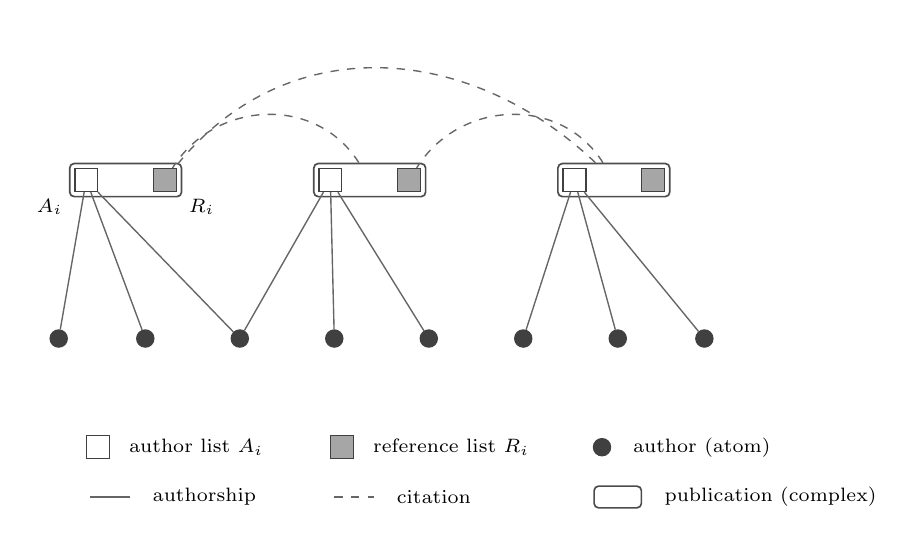
\begin{tikzpicture}[yscale=1.15]
% three publications, each a complex with two internal hyperedges
\foreach \x/\n in {0/1, 3.1/2, 6.2/3} {
  \node[cpx] (A\n) at (\x,0) {};
  \node[cpxb] (R\n) at (\x+1.0,0) {};
  \begin{scope}[on background layer]
    \node[pub,fit=(A\n)(R\n)] (P\n) {};
  \end{scope}
}
\node[lb,anchor=north east] at (-0.18,-0.10) {$A_i$};
\node[lb,anchor=north west] at (1.18,-0.10) {$R_i$};
% authors
\foreach \x/\m in {-0.35/1, 0.75/2, 1.95/3, 3.15/4, 4.35/5, 5.55/6, 6.75/7, 7.85/8}
  \node[atm] (u\m) at (\x,-1.75) {};
\draw[inc] (A1)--(u1) (A1)--(u2) (A1)--(u3) (A2)--(u3) (A2)--(u4) (A2)--(u5)
           (A3)--(u6) (A3)--(u7) (A3)--(u8);
% citations: the cited publication is a vertex of the citing publication's reference list
\draw[incd] (P2) to[out=125,in=55] (R1);
\draw[incd] (P3) to[out=125,in=55] (R2);
\draw[incd] (P3) to[out=140,in=48] (R1);
% legend, laid out below rather than beside so the drawing keeps the page width
\node[cpx]  (l1) at (0.15,-2.95) {}; \node[lb,anchor=west] at (0.42,-2.95) {author list $A_i$};
\node[cpxb] (l2) at (3.25,-2.95) {}; \node[lb,anchor=west] at (3.52,-2.95) {reference list $R_i$};
\node[atm]  (l3) at (6.55,-2.95) {}; \node[lb,anchor=west] at (6.82,-2.95) {author (atom)};
\draw[inc]  (0.05,-3.50)--(0.55,-3.50); \node[lb,anchor=west] at (0.72,-3.50) {authorship};
\draw[incd] (3.15,-3.50)--(3.65,-3.50); \node[lb,anchor=west] at (3.82,-3.50) {citation};
\draw[rounded corners=1.6pt,draw=black!70,line width=.6pt]
  (6.45,-3.62) rectangle (7.05,-3.38);
\node[lb,anchor=west] at (7.22,-3.50) {publication (complex)};
\end{tikzpicture}
\end{adjustbox}
\caption{\textbf{The literature as a chygraph} \citep{vazquez2023pre}. A
publication is a complex, drawn as a rounded box. Its interior is a hypergraph
with two hyperedges: the author list $A_i$ (white) and the reference list $R_i$
(shaded). Authors are atoms and are included in author lists; a citation is the
inclusion of one publication in another publication's reference list, so a
complex is a vertex of a complex. The two hyperedges do not overlap, so the
interior has two components, and the door of entry decides what is reachable.}
\label{fig:publications}
\end{figure}

\section{Graphs, hypergraphs and ubergraphs}

A \emph{graph} $G(V,E)$ is a set of vertices $V$ and a set of edges $E$, each
edge a pair of vertices. It meets neither demand. An edge cannot contain an
edge, and an edge has no interior to give structure to --- it is a pair, and a
pair is exhausted by naming its two members.

A \emph{hypergraph} $H(V,E)$ relaxes the pair: a hyperedge is any subset of $V$,
so an interaction among five things is one hyperedge rather than ten links
\citep{ghoshal2009,battiston2020}. That is real progress, and it is the first
move of the modern higher-order-network literature. It meets the second
demand only barely --- a hyperedge is a flat set, with no internal organisation
--- and it does not meet the first at all. Hyperedges contain vertices. They do
not contain hyperedges. Our paper cannot cite.

The first demand was met by Joslyn and Nowak, who defined \emph{ubergraphs}
\citep{joslyn2017}. We restate their construction in the language this book uses
throughout. Begin by dividing the things in a system into
those we have chosen not to decompose any further --- call them \emph{atoms} ---
and those that are made of other things --- call them \emph{complexes}. Which is
which is a modelling decision, not a fact about the world: an author is an atom
here because we have decided not to model people as made of parts, and nothing
stops someone else deciding otherwise. Then:

\begin{quote}
\emph{An ubergraph} $\mathcal{U}(A,C)$ is a set of atoms $A$ and a set of
complexes $C$, where each complex is a subset of $A\cup C$.
\end{quote}

The clause that does the work is $A\cup C$ rather than $A$. A complex may
contain complexes. Our paper can now cite --- and it still cannot tell its
authors from its references, because a complex is still a flat set. Both lists
are merged into one.

\section{Chygraph definition}
\label{sec:definition}
\index{chygraph|textbf}
\index{complex|textbf}
\index{atom|textbf}
\index{inclusion}

The remaining step is small. If the trouble
is that a complex's interior is a flat set, give the interior the same treatment
we have just given the exterior: make it a hypergraph.

\begin{quote}
\emph{A complex hypergraph} (chygraph) $\chi(A,C)$ is a set of atoms $A$ and a
set of complexes $C$, where each complex is a \emph{hypergraph} whose vertex set
lies in $A\cup C$ \citep{vazquez2023pre}.
\end{quote}

There is a tighter way to say it that will be more convenient from
Chapter~\ref{ch:percolation} onward. An atom is nothing but a complex that
happens to include no complexes, so we need not carry $A$ separately:

\begin{quote}
A chygraph is a set of complexes, where complexes are hypergraphs with a vertex
set in the set of complexes \citep{vazquez2024comnet}.
\end{quote}

Two properties are packed into that sentence. \emph{Self-reference:} complexes
are built from complexes, and are themselves available as building blocks.
\emph{Fine-grained structure:} what is inside a complex is not a heap but a
hypergraph.

Figure~\ref{fig:ladder} puts the three constructions side by side. Each step
buys exactly one thing, and the book needs both.

\begin{figure}[t]
\centering
\begin{adjustbox}{max width=\linewidth}
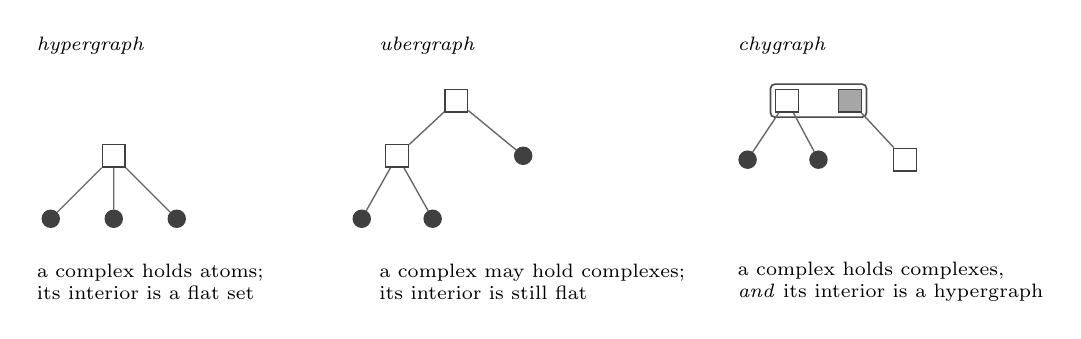
\begin{tikzpicture}[yscale=1.0]
\begin{scope}
  \node[tb,anchor=west] at (-0.2,2.65) {hypergraph};
  \node[cpx] (h) at (0.9,1.25) {};
  \node[atm] (h1) at (0.1,0.45) {}; \node[atm] (h2) at (0.9,0.45) {};
  \node[atm] (h3) at (1.7,0.45) {};
  \draw[inc] (h)--(h1) (h)--(h2) (h)--(h3);
  \node[lb,anchor=west,align=left] at (-0.2,-0.35)
    {a complex holds atoms;\\ its interior is a flat set};
\end{scope}
\begin{scope}[xshift=4.35cm]
  \node[tb,anchor=west] at (-0.2,2.65) {ubergraph};
  \node[cpx] (u) at (0.9,1.95) {};
  \node[cpx] (v) at (0.15,1.25) {};
  \node[atm] (u1) at (1.75,1.25) {};
  \node[atm] (v1) at (-0.3,0.45) {}; \node[atm] (v2) at (0.6,0.45) {};
  \draw[inc] (u)--(v) (u)--(u1) (v)--(v1) (v)--(v2);
  \node[lb,anchor=west,align=left] at (-0.2,-0.35)
    {a complex may hold complexes;\\ its interior is still flat};
\end{scope}
\begin{scope}[xshift=8.9cm]
  \node[tb,anchor=west] at (-0.2,2.65) {chygraph};
  \node[cpx]  (e1) at (0.55,1.95) {};
  \node[cpxb] (e2) at (1.35,1.95) {};
  \begin{scope}[on background layer]\node[pub,fit=(e1)(e2)] (W) {};\end{scope}
  \node[cpx] (w) at (2.05,1.20) {};
  \node[atm] (w1) at (0.05,1.20) {}; \node[atm] (w2) at (0.95,1.20) {};
  \draw[inc] (e1)--(w1) (e1)--(w2) (e2)--(w);
  \node[lb,anchor=west,align=left] at (-0.2,-0.35)
    {a complex holds complexes,\\ \emph{and} its interior is a hypergraph};
\end{scope}
\end{tikzpicture}
\end{adjustbox}
\caption{\textbf{Three constructions, two demands.} A hypergraph's complexes
hold atoms only. An ubergraph's complexes may hold other complexes, but a
complex is still a flat set. A chygraph's complexes hold complexes \emph{and}
carry a hypergraph inside, so a publication can distinguish its author list
(white) from its reference list (shaded). An ubergraph is the special case of a
chygraph in which every interior hypergraph has exactly one hyperedge, so every
result in this book applies to ubergraphs with ``component size'' read as
``cardinality''.}
\label{fig:ladder}
\end{figure}

The literature is now representable without loss. Writing it out,
\begin{equation}
  \chi\Big(A,\ \big\{\,\mathcal{H}_i\big(A_i\cup R_i,\ \{A_i,R_i\}\big)\,\big\}\Big),
  \label{eq:publications}
\end{equation}
where $A$ is the set of authors, $i$ runs over publications, $A_i$ is the
author list of publication $i$ and $R_i$ its reference list. Each publication is
a hypergraph on the vertex set $A_i\cup R_i$ with exactly two hyperedges,
$A_i$ and $R_i$ (Fig.~\ref{fig:publications}). Nothing has been discarded: the
citation network of Fig.~\ref{fig:projections}a, the co-authorship network of
Fig.~\ref{fig:projections}b, the bipartite graph of
Fig.~\ref{fig:projections}c and the hypergraph of Fig.~\ref{fig:projections}d
are all recoverable from Eq.~\eqref{eq:publications} by forgetting, and none of
them can recover any of the others.

\section{The vocabulary}
\label{sec:vocabulary}
\index{cardinality|textbf}
\index{chy-degree|textbf}
\index{excess cardinality|textbf}

A handful of words, all of them intended to be as flat-footed as they sound.

Complex $A$ \emph{includes} complex $B$ when $B$ is in the vertex set of $A$;
equivalently, $B$ is \emph{included in} $A$. An \emph{atom} is a complex that
includes no complexes. The \emph{cardinality} of a complex is the number of
complexes it includes. The \emph{chy-degree} of a complex is the number of
complexes that include it.

Two conventions. First, quantities defined at the
chygraph level get Greek letters, to keep them separate from the same quantities
computed on some graph made out of the chygraph; so the chy-degree is $\kappa$
and never $k$. Second, ``cardinality'' counts what is inside and ``chy-degree''
counts what is outside, and confusing them is the single commonest slip in this
subject. In the literature example, an author's chy-degree is the number of
papers they have written, and a publication's chy-degree is the number of
citations it has received; a publication's cardinality is its number of authors
plus its number of references. An author's $h$-index is a statistic of the
chy-degrees of the complexes that include that atom.

Formally, index the atoms and complexes together as $i=1,\dots,n$ with
$n=|A\cup C|$, and let $C_j$ denote the vertex set of complex $j$. The
\emph{chy-adjacency matrix} is
\begin{equation}
  \alpha_{ij}=\begin{cases}1 & \text{if } i\in C_j,\\ 0 & \text{otherwise,}\end{cases}
  \label{eq:alpha}
\end{equation}
and the chy-degree and cardinality are its two marginals,
\begin{equation}
  \kappa_i=\sum_j\alpha_{ij},\qquad c_j=\sum_i\alpha_{ij}.
  \label{eq:kappa}
\end{equation}
That $\alpha$ is not symmetric --- unlike the adjacency matrix of a graph, which
it otherwise resembles --- is the difference between being inside something and
containing something.

\subsection{The two ways out of a complex}

The rest of the book rests on one sentence, which every recursion in
Chapters~\ref{ch:percolation} to~\ref{ch:overlap} formalises.

\begin{quote}
Standing at a complex, there are exactly two ways to leave it: \emph{up},
through a complex that includes it, or \emph{down}, into the complexes it
includes.
\end{quote}

Up, there are $\kappa$ choices --- one per inclusion --- and they lead to
distinct complexes elsewhere in the chygraph. Down, there is the interior
hypergraph, and this is where the second of the two demands matters:
going down is not a matter of choosing one of $c$ members at random, because the
interior may be several disjoint pieces and only the piece entered is
reachable. Entering a publication as one of its authors reaches the other
authors; entering it as one of its references reaches the other references.
The relevant number is therefore not the cardinality but the size of the
\emph{intra-complex component} arrived in, written $s$
(Fig.~\ref{fig:twoways}).

\begin{figure}[t]
\centering
\begin{adjustbox}{max width=0.92\linewidth}
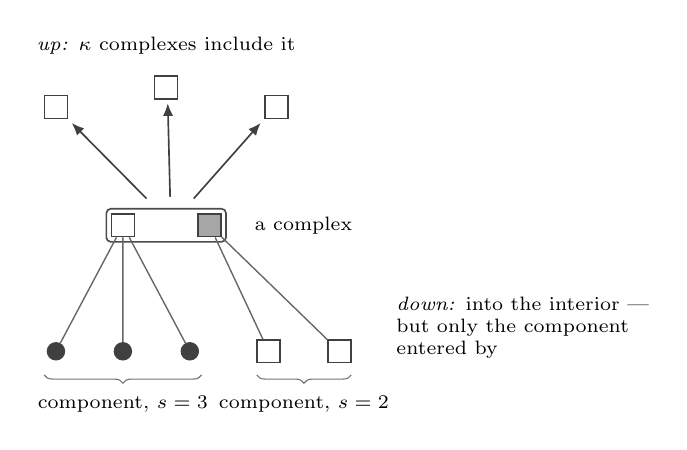
\begin{tikzpicture}
% the complex in the middle
\node[cpx] (E1) at (2.0,0) {}; \node[cpxb] (E2) at (3.1,0) {};
\begin{scope}[on background layer]\node[pub,fit=(E1)(E2)] (P) {};\end{scope}
\node[lb,anchor=west] at (3.55,0.0) {a complex};
% up: complexes that include it
\node[cpx] (Ua) at (1.15,1.5) {}; \node[cpx] (Ub) at (2.55,1.75) {};
\node[cpx] (Uc) at (3.95,1.5) {};
\draw[msg] (2.30,0.34) -- (1.35,1.30);
\draw[msg] (2.60,0.36) -- (2.57,1.55);
\draw[msg] (2.90,0.34) -- (3.75,1.30);
\node[lb,anchor=south,align=center] at (2.55,2.05)
  {\emph{up:} $\kappa$ complexes include it};
% down: the interior, two components
\node[atm] (d1) at (1.15,-1.6) {}; \node[atm] (d2) at (2.0,-1.6) {};
\node[atm] (d3) at (2.85,-1.6) {};
\node[cpx] (d4) at (3.85,-1.6) {}; \node[cpx] (d5) at (4.75,-1.6) {};
\draw[inc] (E1)--(d1) (E1)--(d2) (E1)--(d3) (E2)--(d4) (E2)--(d5);
\draw[decorate,decoration={brace,amplitude=3pt,mirror},black!55]
  (1.0,-1.9) -- (3.0,-1.9);
\draw[decorate,decoration={brace,amplitude=3pt,mirror},black!55]
  (3.7,-1.9) -- (4.9,-1.9);
\node[lb,anchor=north] at (2.0,-2.05) {component, $s=3$};
\node[lb,anchor=north] at (4.3,-2.05) {component, $s=2$};
\node[lb,anchor=west,align=left] at (5.35,-1.30)
  {\emph{down:} into the interior ---\\ but only the component\\ entered by};
\end{tikzpicture}
\end{adjustbox}
\caption{\textbf{The two ways out.} Up, through any of the $\kappa$ complexes
that include this one. Down, into its interior hypergraph --- where what is
reachable is not the whole cardinality $c=5$ but the size $s$ of the component
entered. A publication's author list and reference list are two components of
size $3$ and $2$; arriving as an author, the two other authors are reachable,
not the four other members. Percolation (Chapter~\ref{ch:percolation}) is this
picture with a probability attached to each arrow; the cavity recursion
(Chapter~\ref{ch:statmech}) is this picture with a message.}
\label{fig:twoways}
\end{figure}

Cardinality and component size coincide whenever a complex's interior hypergraph
has a single hyperedge --- which is to say, on ubergraphs, and therefore on
graphs, hypergraphs and every structure in Sec.~\ref{sec:everything} below.
They part company only for genuinely compound complexes like our publications.
The theory is written in terms of $s$ throughout, so both cases are covered by
one calculation, and a reader who only ever cares about hypergraphs may read $s$
as the cardinality, and its excess $\bar s$ of Eq.~\eqref{eq:excess} as
``cardinality minus the one arrived by'', and lose nothing.

\section{Layers}
\label{sec:layers}
\index{layer|textbf}

One more piece of bookkeeping is needed, and it is what makes the construction
computationally workable.

The complexes of a chygraph are usually not statistically alike. In the
literature example, publications and authors are different sorts of object with
different chy-degree distributions, and inside a publication the author list and
the reference list behave differently too. In a multiplex network, a friendship
link and a co-worker link join the same people and are not interchangeable. So
we partition the complexes into \emph{layers}, indexed $l=0,\dots,L-1$, with the
understanding that complexes within a layer are statistically alike and
complexes in different layers need not be.

That is the working definition, and for every calculation in this book it is
all that is needed. The formal version, which fixes how deep a chygraph is
rather than merely how many kinds of thing it contains, is due to
\citet{vazquez2023pre}:

\begin{quote}
\emph{Chygraph length.} Let $\Pi=\Pi_1\cup\dots\cup\Pi_l$ be a partition of the
complex set that is non-intersecting ($\Pi_i\cap\Pi_j=\emptyset$ for $i\ne j$),
hierarchical (if a complex lies in $\Pi_j$ then its vertices lie in
$A\cup(\cup_{k\le j}\Pi_k)$), and statistically homogeneous within each part.
The chygraph length $L(\chi)$ is the largest $l$ over all such partitions.
\end{quote}

The hierarchical clause says that a layer may only be built out of layers below
it, which is what makes ``levels of inclusion'' well defined. Human geography is
the everyday example: people, neighbourhoods, cities, countries, continents ---
five levels, each assembled from the one beneath. The homogeneity clause is what
lets two layers sit at the same level and still be told apart, which is what a
multiplex network needs. The two clauses pull in opposite directions --- one
wants few, deep layers, the other wants many, distinguishable ones --- and the
maximum in the definition resolves them.

No calculation in this book requires computing $L(\chi)$ for a given chygraph. In practice one \emph{chooses} the layers when
setting up the model, and the choice is part of the modelling, exactly as
choosing what counts as an atom was.

\section{Everything is a chygraph}
\label{sec:everything}
\index{hypergraph}
\index{multiplex network}
\index{graph, as a chygraph}

Each structure below is obtained by writing down its layers and their
cardinalities, and nothing else changes. Figure~\ref{fig:mappings} draws them in
a single vocabulary.

\paragraph{A graph} is two layers. Layer $0$ is atoms, one per node. Layer $1$
is complexes of cardinality two, one per link, each containing its two
endpoints. A node's chy-degree is its ordinary degree; a link's chy-degree is
zero, because nothing includes a link.

\paragraph{A hypergraph} is the same with the cardinality freed: layer $1$
complexes contain any number of atoms. A uniform hypergraph fixes that number at
$c$; a clique network --- a graph built by pasting $c$-cliques together --- is
the same chygraph again, because a clique and a hyperedge differ in how they are
drawn and not in what includes what.

\paragraph{A multiplex network} is one atom layer and one complex layer per link
type: friendship in layer $1$, co-working in layer $2$, and so on
\citep{gomez2013,kivela2014}. The atoms are shared, which is exactly what makes
it a multiplex rather than two unrelated networks, and no further apparatus is
required.

\paragraph{Interacting graphs and hypergraphs} need one more layer than one
might guess. Two hypergraphs that interact are: an atom layer and a hyperedge
layer for each, \emph{plus} a layer of hyperedges containing atoms from both
\citep{leicht2009,bianconi2017}. With more than two, one adds a cross layer per
interacting pair.

\paragraph{A clustered graph} becomes a chygraph by \emph{promoting its dense
motifs to complexes}. This is the mapping Part~III rests on. A graph rich in triangles is given two complex layers, one of
cardinality two for the plain links and one of cardinality three for the
triangles \citep{newman2009,karrer2010}. A graph rich in maximal cliques of
assorted sizes gets one layer per size. The triangle has stopped being three
links that happen to close and has become one object, and the loop that made it
a triangle has gone inside the object where the theory can sum over it exactly.
That move is what Chapter~\ref{ch:statmech} is built on, and its price is stated
in Sec.~\ref{sec:treelike} below.

\begin{figure}[t]
\centering
\begin{adjustbox}{max width=\linewidth}
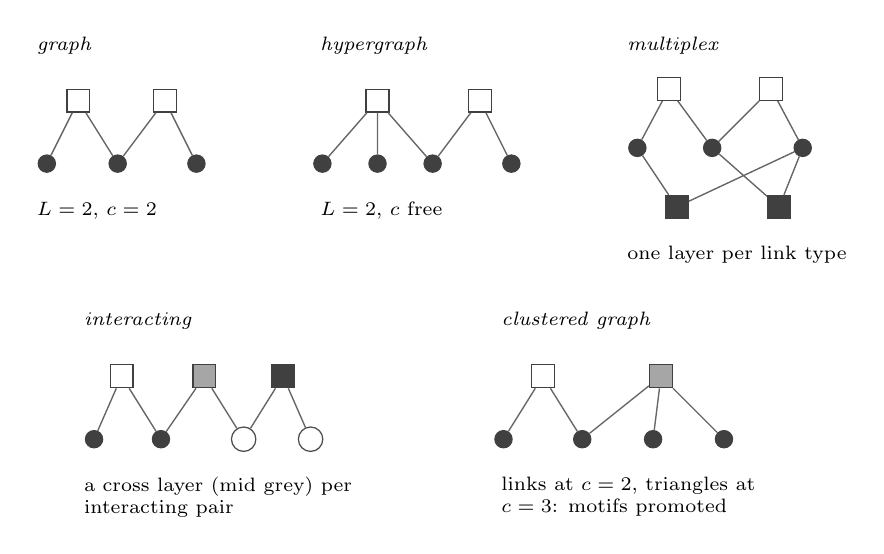
\begin{tikzpicture}
% ---------- row 1: graph, hypergraph, multiplex ----------
\begin{scope}
  \node[tb,anchor=west] at (-0.3,1.75) {graph};
  \node[cpx] (g1) at (0.35,1.05) {}; \node[cpx] (g2) at (1.45,1.05) {};
  \node[atm] (n1) at (-0.05,0.25) {}; \node[atm] (n2) at (0.85,0.25) {};
  \node[atm] (n3) at (1.85,0.25) {};
  \draw[inc] (g1)--(n1) (g1)--(n2) (g2)--(n2) (g2)--(n3);
  \node[lb,anchor=west] at (-0.3,-0.35) {$L=2$, $c=2$};
\end{scope}
\begin{scope}[xshift=3.6cm]
  \node[tb,anchor=west] at (-0.3,1.75) {hypergraph};
  \node[cpx] (H1) at (0.55,1.05) {}; \node[cpx] (H2) at (1.85,1.05) {};
  \node[atm] (m1) at (-0.15,0.25) {}; \node[atm] (m2) at (0.55,0.25) {};
  \node[atm] (m3) at (1.25,0.25) {}; \node[atm] (m4) at (2.25,0.25) {};
  \draw[inc] (H1)--(m1) (H1)--(m2) (H1)--(m3) (H2)--(m3) (H2)--(m4);
  \node[lb,anchor=west] at (-0.3,-0.35) {$L=2$, $c$ free};
\end{scope}
\begin{scope}[xshift=7.5cm]
  \node[tb,anchor=west] at (-0.3,1.75) {multiplex};
  \node[cpx]  (M1) at (0.35,1.20) {}; \node[cpx]  (M2) at (1.65,1.20) {};
  \node[atm] (p1) at (-0.05,0.45) {}; \node[atm] (p2) at (0.90,0.45) {};
  \node[atm] (p3) at (2.05,0.45) {};
  \node[cpxc] (M3) at (0.45,-0.30) {}; \node[cpxc] (M4) at (1.75,-0.30) {};
  \draw[inc] (M1)--(p1) (M1)--(p2) (M2)--(p2) (M2)--(p3)
             (M3)--(p1) (M3)--(p3) (M4)--(p2) (M4)--(p3);
  \node[lb,anchor=west] at (-0.3,-0.90) {one layer per link type};
\end{scope}
% ---------- row 2: interacting, clustered graph ----------
\begin{scope}[yshift=-3.5cm,xshift=0.6cm]
  \node[tb,anchor=west] at (-0.3,1.75) {interacting};
  \node[cpx]  (I1) at (0.30,1.05) {}; \node[cpxb] (I3) at (1.35,1.05) {};
  \node[cpxc] (I2) at (2.35,1.05) {};
  \node[atm] (q1) at (-0.05,0.25) {}; \node[atm] (q2) at (0.80,0.25) {};
  \node[nd]  (q3) at (1.85,0.25) {}; \node[nd]  (q4) at (2.70,0.25) {};
  \draw[inc] (I1)--(q1) (I1)--(q2) (I2)--(q3) (I2)--(q4)
             (I3)--(q2) (I3)--(q3);
  \node[lb,anchor=west,align=left] at (-0.3,-0.48)
    {a cross layer (mid grey) per\\ interacting pair};
\end{scope}
\begin{scope}[yshift=-3.5cm,xshift=5.9cm]
  \node[tb,anchor=west] at (-0.3,1.75) {clustered graph};
  \node[cpx]  (T1) at (0.35,1.05) {};
  \node[cpxb] (T2) at (1.85,1.05) {};
  \node[atm] (r1) at (-0.15,0.25) {}; \node[atm] (r2) at (0.85,0.25) {};
  \node[atm] (r3) at (1.75,0.25) {}; \node[atm] (r4) at (2.65,0.25) {};
  \draw[inc] (T1)--(r1) (T1)--(r2) (T2)--(r2) (T2)--(r3) (T2)--(r4);
  \node[lb,anchor=west,align=left] at (-0.3,-0.48)
    {links at $c=2$, triangles at\\ $c=3$: motifs promoted};
\end{scope}
\end{tikzpicture}
\end{adjustbox}
\caption{\textbf{One object, five structures.} Circles are atoms, rectangles
are complexes, and shading distinguishes layers; a line is an inclusion. In the
interacting panel the two hypergraphs' atoms are told apart by fill, and the
mid-grey complexes are the cross layer that contains atoms of both. Nothing changes from panel to panel except which layers exist and
what cardinalities they carry. This is the claim the rest of the book relies on:
a calculation done once on the chygraph is a calculation done for all five, and
the specialisation is substitution rather than rederivation.}
\label{fig:mappings}
\end{figure}

The list is the argument for the whole construction. The
higher-order-network literature has produced a separate percolation calculation
for hypergraphs, for multiplex networks, for interacting networks, for
interdependent networks, for simplicial complexes, and for clustered graphs, and
the number of independent derivations has been growing faster than anyone's
ability to hold them in one head \citep{battiston2020,bianconi2021}. If all six
are chygraphs, one calculation covers them, and the differences between them
become differences in what one substitutes at the end. Chapter~\ref{ch:percolation}
carries that out.

\section{Two ways to draw the same thing}
\label{sec:drawing}
\index{inclusion diagram}

Figures~\ref{fig:publications} and~\ref{fig:mappings} draw a complex as a
\emph{node} of its own, with lines running to what it includes. Every figure
after this chapter draws a complex as a \emph{box around} what it includes.
These are the same object. Figure~\ref{fig:twodrawings} puts the two side by
side once, so that neither reads as a new construction later.

The inclusion drawing is complete and scales badly: it puts every complex and
every inclusion on the page, and it becomes unreadable at a couple of dozen
complexes. The spatial drawing is compact and incomplete: it can only show a
complex as a box when the complex's members can be drawn adjacent, which
fails as soon as two complexes share more than one atom --- precisely the
situation of Sec.~\ref{sec:treelike}. Use the first when the question is what
includes what, the second when the question is what is near what.

\begin{figure}[t]
\centering
\begin{adjustbox}{max width=0.9\linewidth}
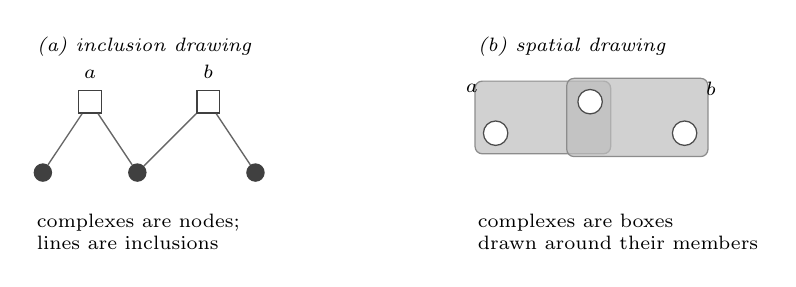
\begin{tikzpicture}
\begin{scope}
  \node[tb,anchor=west] at (-0.2,2.15) {(a) inclusion drawing};
  \node[cpx] (A) at (0.6,1.45) {}; \node[cpx] (B) at (2.1,1.45) {};
  \node[lb,anchor=south] at (0.6,1.62) {$a$};
  \node[lb,anchor=south] at (2.1,1.62) {$b$};
  \node[atm] (x1) at (0.0,0.55) {}; \node[atm] (x2) at (1.2,0.55) {};
  \node[atm] (x3) at (2.7,0.55) {};
  \draw[inc] (A)--(x1) (A)--(x2) (B)--(x2) (B)--(x3);
  \node[lb,anchor=west,align=left] at (-0.2,-0.20)
    {complexes are nodes;\\ lines are inclusions};
\end{scope}
\begin{scope}[xshift=5.6cm]
  \node[tb,anchor=west] at (-0.2,2.15) {(b) spatial drawing};
  % the two complexes are drawn at different heights and different fills, so
  % that the atom they share is visibly in both rather than in one long blob
  \node[nd] (y1) at (0.15,1.05) {}; \node[nd] (y2) at (1.35,1.45) {};
  \node[nd] (y3) at (2.55,1.05) {};
  \begin{scope}[on background layer]
    \node[cx,fill=black!26,fill opacity=0.7,fit=(y1)(y2)] {};
    \node[cx,fill=black!26,fill opacity=0.7,inner sep=3.8pt,fit=(y2)(y3)] {};
  \end{scope}
  \node[lb,anchor=east] at (0.05,1.62) {$a$};
  \node[lb,anchor=west] at (2.70,1.62) {$b$};
  \node[lb,anchor=west,align=left] at (-0.2,-0.20)
    {complexes are boxes\\ drawn around their members};
\end{scope}
\end{tikzpicture}
\end{adjustbox}
\caption{\textbf{The same chygraph twice.} Three atoms and two complexes, $a$
and $b$, the middle atom belonging to both. The inclusion drawing (a) is used in
this chapter because the question here is what includes what; the spatial
drawing (b) is used everywhere afterwards because the question there is what a
message can reach. Neither adds anything to the other.}
\label{fig:twodrawings}
\end{figure}

\section{Random chygraphs}
\label{sec:ensembles}
\index{random chygraph|textbf}
\index{ensemble}

The rest of the book computes averages over ensembles rather than properties of
one object, so we need to say what specifying an ensemble amounts to. It amounts
to specifying, for every ordered pair of layers, how many complexes of one layer
attach to a complex of the other, in each of the two directions of
Sec.~\ref{sec:vocabulary} --- and that is all.

Let $\Phi^l_k(x)$ be the probability generating function of the number of
layer-$k$ complexes that include a layer-$l$ complex, and $G^l_k(y)$ that of the
number of layer-$k$ complexes in the intra-complex component of a layer-$l$
complex, entered at a given vertex. Write $\bar\Phi^l_k$ and $\bar G^l_k$ for
the corresponding \emph{excess} functions --- the same counts taken from a
complex reached along an inclusion, with the inclusion used to arrive not
counted again. Up and down, ordinary and excess: four families of functions, one
per direction per situation.

Their first derivatives at $1$ are the four moment matrices that will run
through every chapter:
\begin{align}
  \Phi^{l\prime}_k(1)&=\ave{\kappa}_{lk}, &
  \bar\Phi^{l\prime}_k(1)&=\ave{\kbar}_{lk},\nonumber\\
  G^{l\prime}_k(1)&=\ave{s}_{lk}, &
  \bar G^{l\prime}_k(1)&=\ave{\sbar}_{lk},
  \label{eq:moments}
\end{align}
with the excess averages given, as usual for a size-biased count, by
\begin{equation}
  \ave{\kbar}_{lk}=\frac{\ave{\kappa(\kappa-1)}_{lk}}{\ave{\kappa}_{lk}},
  \qquad
  \ave{\sbar}_{lk}=\frac{\ave{s(s-1)}_{lk}}{\ave{s}_{lk}}.
  \label{eq:excess}
\end{equation}

Four $L\times L$ matrices, then, summarise a chygraph at the level of first
moments: $\ave{\kappa}$, $\ave{\kbar}$, $\ave{s}$, $\ave{\sbar}$. Whatever the sizes of the complexes, whatever
the depth of the inclusion hierarchy, the first-moment description of the
ensemble is four matrices whose dimension is the number of \emph{layers} --- two
for a graph, three for a two-layer multiplex --- and not the number of complexes
or their cardinality. Chapter~\ref{ch:percolation} shows that the percolation
threshold of every structure in Sec.~\ref{sec:everything} is fixed by these four
matrices alone; Chapter~\ref{ch:giant} shows precisely what they fail to
determine, which is everything about the transition except where it is.

Two caveats, stated here so they are not sprung later. Equation~\eqref{eq:moments}
takes the generating functions to factorise over target layers --- a complex's
participation in one layer independent of its participation in another --- which
covers every mapping in Sec.~\ref{sec:everything} but is a genuine restriction,
lifted in Sec.~\ref{sec:joint}. And moments are moments: two ensembles can agree
on all four matrices and disagree about the shape of the transition, which is
the subject of Chapter~\ref{ch:giant} and not a defect to be repaired.

\section{Treelike over complexes, and what it costs}
\label{sec:treelike}
\index{treelike|textbf}
\index{overlap!between complexes}

We close the chapter with the property that motivates everything after
Chapter~\ref{ch:percolation}, and with its price, which is structural rather
than a matter of care.

The methods of this book --- generating functions for percolation, the cavity
recursion for statistical mechanics --- require that the object they run on be
locally treelike: that following inclusions away from a complex, one does not
come back. Real graphs are not treelike: the neighbours of a node are neighbours
of one another, and the triangle they form is a loop of length three, the
shortest there is.

Promote that triangle to a complex, though, and the loop is gone from the
structure \emph{over} complexes. It has not been discarded --- it is inside the
complex, where Chapter~\ref{ch:statmech} sums over it exactly at a cost that
depends on the cardinality and on nothing else. What was an obstruction has
become an interior. This is the bargain the book explores, and Fig.~\ref{fig:price}a
is the good case.

Figure~\ref{fig:price}b is the bad one. If two complexes share \emph{two} atoms
rather than one, then there is a loop that promotion did not absorb: leave the
first complex through one shared atom, cross the second complex, and come back
through the other. Over complexes, that is a loop of length two, and the
recursion will double-count it.

\paragraph{The pairwise test is necessary and not sufficient.} It is convenient
to read the condition as the single question ``do two complexes ever share two
atoms?'', and that is how the rest of this book applies it. On an ensemble the
reading is safe: the random chygraphs of Part~II are locally treelike in the
full sense, and a loop of any length is a rare event. On a \emph{given} network
it is not. A loop can run through three or more complexes, each meeting the next
in a single atom and no pair sharing two, so that the pairwise question is
answered ``no'' and the structure over complexes still closes on itself. Four
triangles glued in a ring at single vertices do exactly that, and the recursion
is wrong on them; Section~\ref{sec:mergeerror} draws the object and prices the
error. What the recursion needs is that the incidence structure be a forest, of
which sharing at most one atom is a consequence rather than a guarantee.

\begin{figure}[t]
\centering
\begin{adjustbox}{max width=0.94\linewidth}
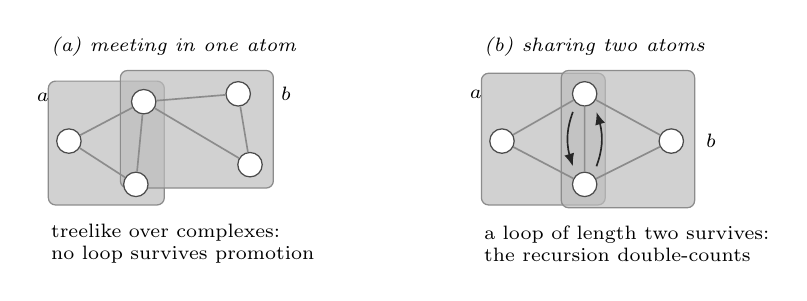
\begin{tikzpicture}
\begin{scope}
  \node[tb,anchor=west] at (-0.2,2.55) {(a) meeting in one atom};
  \node[nd] (a1) at (0.15,1.35) {}; \node[nd] (a2) at (1.10,1.85) {};
  \node[nd] (a3) at (1.00,0.80) {};
  \node[nd] (a4) at (2.30,1.95) {}; \node[nd] (a5) at (2.45,1.05) {};
  \draw[lnk] (a1)--(a2)--(a3)--(a1) (a2)--(a4)--(a5)--(a2);
  \begin{scope}[on background layer]
    \node[cx,fill=black!26,fill opacity=0.7,fit=(a1)(a2)(a3)]{};
    \node[cx,fill=black!26,fill opacity=0.7,inner sep=3.8pt,fit=(a2)(a4)(a5)]{};
  \end{scope}
  \node[lb,anchor=east] at (0.02,1.90) {$a$};
  \node[lb,anchor=west] at (2.72,1.95) {$b$};
  \node[lb,anchor=west,align=left] at (-0.2,0.05)
    {treelike over complexes:\\ no loop survives promotion};
\end{scope}
\begin{scope}[xshift=5.5cm]
  \node[tb,anchor=west] at (-0.2,2.55) {(b) sharing two atoms};
  \node[nd] (b1) at (0.15,1.35) {}; \node[nd] (b2) at (1.20,1.95) {};
  \node[nd] (b3) at (1.20,0.80) {}; \node[nd] (b4) at (2.30,1.35) {};
  \draw[lnk] (b1)--(b2)--(b3)--(b1) (b2)--(b4)--(b3);
  \begin{scope}[on background layer]
    \node[cx,fill=black!26,fill opacity=0.7,fit=(b1)(b2)(b3)]{};
    \node[cx,fill=black!26,fill opacity=0.7,inner sep=3.8pt,fit=(b2)(b3)(b4)]{};
  \end{scope}
  \node[lb,anchor=east] at (0.02,1.95) {$a$};
  \node[lb,anchor=west] at (2.62,1.35) {$b$};
  % the surviving loop: out of a through one shared atom, back through the other
  \draw[msg,black!85] (1.05,1.72) to[out=250,in=110] (1.05,1.03);
  \draw[msg,black!85] (1.35,1.03) to[out=70,in=290] (1.35,1.72);
  \node[lb,anchor=west,align=left] at (-0.2,0.05)
    {a loop of length two survives:\\ the recursion double-counts};
\end{scope}
\end{tikzpicture}
\end{adjustbox}
\caption{\textbf{The bargain and its price.} (a) Two triangles, $a$ and $b$,
meeting at one atom. Promoted to complexes, the structure over complexes is a
tree, and every loop of the underlying graph now lives inside a complex.
(b) Two triangles sharing an edge --- two atoms. Promotion removes the loops
inside each triangle and leaves a loop \emph{between} them, traced by the
arrows, which the theory of Chapters~\ref{ch:percolation}--\ref{ch:satisfiability}
does not see. Chapter~\ref{ch:overlap} measures what this costs on real
clustered graphs, and Chapters~\ref{ch:gbp} and~\ref{ch:metacomplex} are the two
repairs.}
\label{fig:price}
\end{figure}

So the condition is easy to state and easy to check, with the caveat above kept
in view: \textbf{a chygraph is locally treelike only if its complexes meet in at
most one atom}, and on the random ensembles of Part~II that necessary condition
is sufficient as well. Uniform
hypergraphs drawn from a configuration model satisfy it with probability
approaching one. Multiplex and interacting networks satisfy it by construction.
Graphs decorated with triangles in the manner of \citet{newman2009} satisfy it
because the triangles are placed independently. What does not satisfy it is the
case one most wants: the maximal cliques of a real, geometrically clustered
graph, which overlap along edges as a matter of course
\citep{friedrich2015}.

This is stated in the chapter that defines the object rather than in a remark
at the end of the book. The next eleven chapters develop what the construction
buys; Chapter~\ref{ch:overlap} returns to Fig.~\ref{fig:price}b, measures the damage
on hyperbolic random graphs --- between $77$ and $100$ per cent of the answer
recovered --- and describes what would be needed to recover the rest. Clustering
is not one obstruction but a hierarchy of them: promoting
triangles removes the loops within triangles and exposes the loops between them.
Whether that hierarchy terminates usefully is, as of this writing, open.


% sources
% - manuscript 1 (Phys. Rev. E 107, 024316), Sec. II "Key definitions"
% - manuscript 2 (J. Complex Netw. 2024, cnae047), Sec. 2 "Chygraphs"

% Three lines at \Huge on this measure -- "Chygraph representation" is a
% shade too wide for one. Broken by hand so the last line is a phrase rather
% than an orphaned "systems"; the optional argument keeps the contents and
% the running head on one line.
\chapter[Chygraph representation of real systems]{Chygraph\\representation\\of real systems}
\label{ch:data}

Chapter~\ref{ch:chygraphs} defined an object. In this chapter we ask where to
get hold of it. Everything measured here is new; the
worked example of a publication as a complex is Chapter~\ref{ch:chygraphs}'s,
and drawn rather than measured. There are exactly two routes, they behave very differently, and
which of the two applies decides in advance how well the theory of the next ten
chapters will work on the data, so it comes before the theory rather than
after.

The first route is the easy one. Some systems record their groups. A paper
lists its authors, a purification recovers a set of proteins together, a
reaction names its substrates, a work package names its predecessors. Where the
groups are in the data, the chygraph is read straight off them, and the only
decisions are which layers to use.

The second route is the one most people are on. There is a graph, and nothing
else --- a list of pairs, with whatever produced them long since discarded. Then
the complexes have to be \emph{found}, and the natural candidates are the dense
motifs: the maximal cliques. This route works, but it works to a degree that
varies enormously from one network to another, and Sec.~\ref{sec:promoting}
measures how much on ten real networks.

There is also a third thing one does, which is not a route into real data at
all but is needed throughout the book: generating random chygraphs to check the
theory against. That is Sec.~\ref{sec:sampling}.

\begin{figure}[t]
\centering
\begin{adjustbox}{max width=\linewidth}
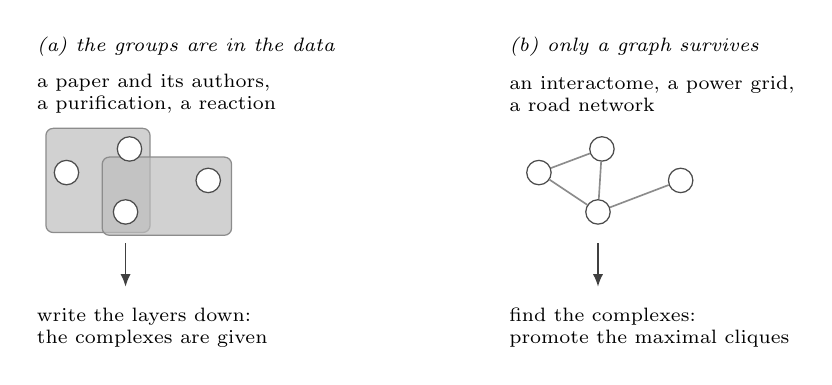
\begin{tikzpicture}
% ---------------- route 1: the groups are in the data
\begin{scope}
  \node[tb,anchor=west] at (-0.2,3.15) {(a) the groups are in the data};
  \node[lb,anchor=west,align=left] at (-0.2,2.55)
    {a paper and its authors,\\ a purification, a reaction};
  \node[nd] (s1) at (0.30,1.55) {}; \node[nd] (s2) at (1.10,1.85) {};
  \node[nd] (s3) at (1.05,1.05) {}; \node[nd] (s4) at (2.10,1.45) {};
  \begin{scope}[on background layer]
    \node[cx,fill=black!26,fill opacity=0.7,fit=(s1)(s2)(s3)]{};
    \node[cx,fill=black!26,fill opacity=0.7,inner sep=3.8pt,fit=(s3)(s4)]{};
  \end{scope}
  \draw[msg] (1.05,0.65) -- (1.05,0.10);
  \node[lb,anchor=west,align=left] at (-0.2,-0.42)
    {write the layers down:\\ the complexes are given};
\end{scope}
% ---------------- route 2: only a graph
\begin{scope}[xshift=6.0cm]
  \node[tb,anchor=west] at (-0.2,3.15) {(b) only a graph survives};
  \node[lb,anchor=west,align=left] at (-0.2,2.55)
    {an interactome, a power grid,\\ a road network};
  \node[nd] (t1) at (0.30,1.55) {}; \node[nd] (t2) at (1.10,1.85) {};
  \node[nd] (t3) at (1.05,1.05) {}; \node[nd] (t4) at (2.10,1.45) {};
  \draw[lnk] (t1)--(t2)--(t3)--(t1) (t3)--(t4);
  \draw[msg] (1.05,0.65) -- (1.05,0.10);
  \node[lb,anchor=west,align=left] at (-0.2,-0.42)
    {find the complexes:\\ promote the maximal cliques};
\end{scope}
\end{tikzpicture}
\end{adjustbox}
\caption{\textbf{Two routes in.} (a) When the data records its groups, the
complexes are given and the modelling is a choice of layers. (b) When only a
list of pairs survives, the complexes must be found, and the maximal cliques are
the natural candidates. Route (b) is a reconstruction and can fail;
Sec.~\ref{sec:promoting} measures how badly, and finds that the worst case is a
network that was on route (a) before somebody flattened it.}
\label{fig:tworoutes}
\end{figure}

\section{Systems whose interactions are not pairwise}
\label{sec:systems}

Four families of system, chosen because between them they cover most of what
anybody wants to do with this construction, and because they differ in exactly
the way that matters --- how much of the group structure survives into the file
that is finally distributed.

\paragraph{Papers and their authors.} Treated at length in
Sec.~\ref{sec:paper}. Atoms are authors, complexes are publications, the
interior hypergraph of a publication has two hyperedges --- author list and
reference list --- and a citation is a complex included in a complex. Of the
four families this is the only one that genuinely needs the interior to be a
hypergraph rather than a flat set, and it is the one that needs inclusion to
recurse. It is the reason the definition is what it is.

\paragraph{Proteins in complexes.} A protein complex is a set of proteins that
act as a unit --- the ribosome, the proteasome, a transcription factor assembly.
Affinity purification recovers such a set in one experiment: a bait protein is
pulled down and everything bound to it comes with it. That is group-level data
in the most literal sense, and the natural chygraph has proteins as atoms and
purifications as complexes, with one layer per experiment type. Two-hybrid
screening, by contrast, tests one pair at a time and produces genuinely pairwise
data. The two kinds of experiment therefore produce different objects, and
Sec.~\ref{sec:promoting} shows they behave completely differently under
promotion.

\paragraph{Reactions and their species.} A chemical reaction consumes some
species and produces others, and the natural complex has an interior with two
hyperedges --- substrates and products --- exactly like a publication's authors
and references. Metabolic networks are routinely drawn as graphs of species
joined when a reaction connects them, which loses the stoichiometry, the
direction and the grouping in one move.

\paragraph{Activities and their dependencies.} A project schedule is a set of
activities and the logical constraints between them, and constraints are often
group-level: an activity may start when \emph{all} of a set of predecessors have
finished, or when \emph{any} one has. Those are two different interiors on the
same complex --- a distinction Chapter~\ref{ch:giant} makes precise as AND-logic
against OR-logic, and one that no pairwise graph can carry.

Table~\ref{tab:systems} collects the four, together with what the pairwise
graph keeps of each and what it throws away.

\begin{table}[t]
\centering\small
\begin{tabular}{lll}
\hline\hline
system & atoms & complexes\\
\hline
literature & authors & publications (authors $+$ references)\\
proteomics & proteins & purifications, or screened pairs\\
metabolism & species & reactions (substrates $+$ products)\\
projects & activities & dependency sets (AND or OR)\\
\hline\hline
\end{tabular}
\caption{\textbf{Four systems, one construction.} In each case the complexes are
what the experiment or the record actually produces, and the pairwise graph is
what is left after the grouping has been thrown away.}
\label{tab:systems}
\end{table}

\section{Reading the layers off group data}
\label{sec:layers-data}
\index{group data}

When the groups are given, building the chygraph is bookkeeping, and there are
three decisions to make.

\emph{What is an atom.} Whatever the modelling declines to decompose further.
This is a
modelling choice and it should be made once, explicitly, because everything
downstream inherits it.

\emph{What the layers are.} One layer per statistically distinct kind of
complex. Distinctness is the operative word: two kinds of complex belong in
different layers when their chy-degree distributions or cardinality
distributions differ, and in the same layer when they do not. Two-hybrid
interactions and affinity purifications are different layers. Author lists and
reference lists are different layers. A hypergraph with a broad spread of
cardinalities takes one layer per cardinality, which sounds extravagant and is
not, because $L$ enters the theory only as the size of an $L\times L$
determinant.

\emph{Whether the layers are independent.} The theory of
Chapters~\ref{ch:percolation} and~\ref{ch:statmech} assumes that a complex's
participation in one layer says nothing about its participation in another,
so that the generating functions factorise. That is often false in data --- a
protein in many purifications is usually also in many two-hybrid pairs --- and
the repair is to replace the marginals by a joint $\Phi$, with the
unconditional first moments replaced by inclusion-biased second moments.
Chapter~\ref{ch:giant} does that in general and shows it matters: two ensembles
with \emph{identical} marginals can have different thresholds. So this decision
is not cosmetic, and the way to make it is to measure the correlation between
layer memberships before assuming it away.

One rule of thumb, with the evidence for it in Sec.~\ref{sec:promoting}:
\textbf{where the group data exists, use it; do not flatten it to a graph and
then try to recover the groups.} The flattening is not invertible, and what
comes back is worse than either the graph or the groups.

\section{Promoting the cliques of a real graph}
\label{sec:promoting}
\index{clique promotion|textbf}
\index{configuration model}
\index{clustering!manufactured by a null model}

On the other route a graph is given and a chygraph has to be built from it. The
recipe of
Sec.~\ref{sec:everything} says to promote the dense motifs, and with no
information about which motifs are meaningful, the maximal cliques are the
default choice: a maximal clique is a set of nodes all of which are joined, not
contained in any larger such set, and every edge lies in at least one.

Two questions decide whether this works, and both are measurable before any
physics is done.

The first is whether the resulting ensemble has finite moments. The threshold
tensor of Chapter~\ref{ch:percolation} needs the excess cardinality seen from a
member,
\begin{equation}
  \bar s=\frac{\ave{c^{2}}}{\ave{c}}-1,
  \label{eq:sbar-data}
\end{equation}
to be finite --- which is to say, the clique-size distribution needs a converged
second moment. The reference value is easy to remember: a graph with no
clustering at all has almost every edge in a maximal clique of size two, and
sits at $\bar s\approx1$.

The second is whether the cliques overlap. Section~\ref{sec:treelike} established
that a chygraph is treelike only when its complexes meet in at most one atom, so
the diagnostic is the fraction of intersecting clique pairs that share two or
more atoms. Call it $\mathrm{shared}_{2+}$. It is zero for a treelike chygraph
and one for a family in which every intersection is an edge or larger.

Table~\ref{tab:real} and Figure~\ref{fig:realoverlap} report both for ten real
networks --- eight protein interaction datasets, a power grid and a road network
--- each carried alongside its degree-matched configuration model, which
rewires everything at fixed degree sequence. (Whether that destroys the
clustering, which is what one usually assumes it does, turns out to be the third
finding below.)

\begin{table}[t]
\centering\small
\begin{tabular}{lrrrrrr}
\hline\hline
 & & & \multicolumn{2}{c}{$\bar s$} & \multicolumn{2}{c}{shared$_{2+}$}\\
network & $\ave{k}$ & $C$ & real & ctrl & real & ctrl\\
\hline
Collins yeast & 16.57 & 0.648 & 21.91 & 1.97 & 0.903 & 0.055\\
Yeast (Y2H) & 2.67 & 0.071 & 1.15 & 1.02 & 0.014 & 0.001\\
Human (Vidal) & 4.32 & 0.072 & 1.26 & 1.09 & 0.022 & 0.007\\
Human (Stelzl) & 3.85 & 0.006 & 1.05 & 1.21 & 0.003 & 0.022\\
Human (Figeys) & 5.79 & 0.040 & 1.21 & 2.37 & 0.022 & 0.155\\
PDZ domains & 2.60 & 0.007 & 1.01 & 1.10 & 0.000 & 0.015\\
C. elegans WI8 & 3.20 & 0.022 & 1.13 & 1.11 & 0.014 & 0.012\\
C. elegans 2007 & 2.71 & 0.017 & 1.09 & 1.12 & 0.010 & 0.014\\
Power grid & 2.67 & 0.080 & 1.14 & 1.00 & 0.016 & 0.000\\
Euroroad & 2.51 & 0.019 & 1.04 & 1.00 & 0.001 & 0.000\\
\hline\hline
\end{tabular}

\caption{\textbf{The chygraph a real graph has.} Maximal cliques promoted to
complexes, for ten networks and for their degree-matched configuration models
(``ctrl'', mean of three realisations). $C$ is the average clustering
coefficient, $\bar s$ the excess cardinality of Eq.~\eqref{eq:sbar-data}, and
$\mathrm{shared}_{2+}$ the fraction of intersecting complex pairs sharing two or
more atoms --- the pairs the construction cannot represent. Generated by
\code{figs/real\_chygraphs.py}.}
\label{tab:real}
\end{table}

\begin{figure}[t]
\centering
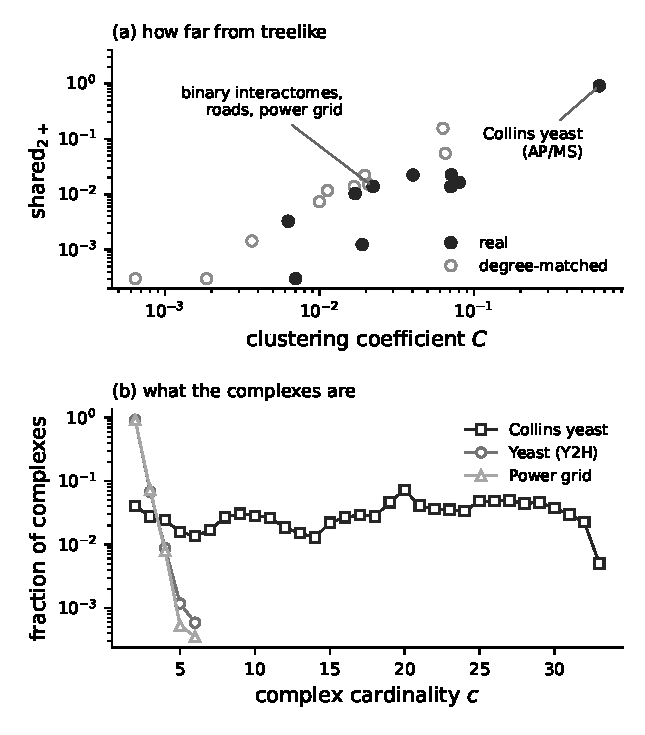
\includegraphics[width=0.86\linewidth]{figs/fig-real-overlap.pdf}
\caption{\textbf{How far from treelike, and why.} (a) Overlap against clustering
for the ten networks of Table~\ref{tab:real}, filled for the real network and
open for its degree-matched control. (b) The cardinality distribution of the
promoted complexes. Two-hybrid interactomes and infrastructure networks are
almost entirely complexes of cardinality two with a thin tail; the
purification-derived network is a different object altogether, with complexes
out to cardinality $33$ and no characteristic size.}
\label{fig:realoverlap}
\end{figure}

Three findings follow, and the third is the least expected.

\paragraph{Most real graphs promote almost perfectly.} The two-hybrid
interactomes, the power grid and the road network all sit at $\bar s$ between
$1.01$ and $1.26$ --- within about a quarter of the clustering-free reference
--- and at $\mathrm{shared}_{2+}$ between $0.000$ and $0.022$. Fewer than one
intersecting clique pair in forty-four shares an edge. For these networks the
chygraph of maximal cliques is treelike for practical purposes, and the theory
of the next ten chapters applies to them essentially without correction. The
obstruction Chapter~\ref{ch:overlap} is about is therefore specific rather than
generic, and one can tell in advance whether one has it.

\paragraph{One network fails completely.} The
Collins yeast dataset sits at $\bar s=21.9$ against a control of $1.97$, at
$\mathrm{shared}_{2+}=0.903$, and its average edge is covered by $114$ distinct
maximal cliques. Nine intersecting clique pairs in ten share an edge or more.
Promotion has failed categorically.

Collins \emph{et al.} measured
co-complex associations by affinity purification and mass spectrometry: a
purification recovers a group of proteins together, and the public network
records that group by joining all pairs within it. The graph is a union of
cliques, one per purification, and it is a union of \emph{overlapping} cliques
because proteins belong to several complexes. So the dataset was on route (a) of
Figure~\ref{fig:tworoutes}, and somebody flattened it onto route (b). Trying to
recover the groups by clique promotion is an attempt to invert that flattening,
and Figure~\ref{fig:realoverlap}b shows what comes back: a cardinality
distribution running to $33$ with no characteristic size, because the maximal
cliques of a union of overlapping cliques are not the original groups but every
combination the overlaps permit.

That is the rule of Sec.~\ref{sec:layers-data} arriving as a measurement. The
underlying purifications would have made a perfectly good chygraph with a
handful of layers and modest cardinalities. The flattened graph does not, and no
amount of care in the promotion step will repair it, because the information was
destroyed before the file was written.

\paragraph{The control is not always the cleaner object.} Destroying the
clustering might be expected only to reduce the overlap, so that the
configuration model would always sit below the real network in
Figure~\ref{fig:realoverlap}a. In four of the ten it sits \emph{above}. For the
Figeys human interactome the control's $\mathrm{shared}_{2+}$ is $0.155$ against
the real network's $0.022$, a factor of seven the wrong way, and its $\bar s$ is
$2.37$ against $1.21$.

The mechanism is degree heterogeneity. A configuration model with a heavy tail
gives its hubs so many neighbours that some of those neighbours are shared by
chance, and shared neighbours are triangles, and triangles are cliques of
cardinality three. So the control does not have zero clustering; it has however
much its degree sequence manufactures, and that quantity grows with the degree
heterogeneity $\ave{k^{2}}/\ave{k}$. The Figeys network is the most heterogeneous of
the ten by a wide margin --- $\ave{k^{2}}/\ave{k}=56$, half again the next
largest and four times the median --- and it is the one whose control overlaps
most, at $0.155$.

Which of the two wins is then a race between the clustering a network really has
and the clustering its degree sequence would manufacture anyway. The control
wins on Stelzl ($C=0.006$), PDZ ($C=0.007$), Figeys ($C=0.040$) and, narrowly,
the 2007 \emph{C. elegans} screen ($C=0.017$, $0.014$ against $0.010$): all
networks with little real clustering and enough heterogeneity to manufacture
some. It loses on Euroroad, which has almost no clustering either ($C=0.019$)
but a light tail --- $\ave{k^{2}}/\ave{k}=3.1$, the lowest here --- so its
control manufactures nothing at all and returns $\mathrm{shared}_{2+}=0.000$.
And it loses on every network with real clustering to spare, Vidal and the power
grid among them.

The practical consequence is a caution rather than a result, and it applies to
every degree-matched comparison in this book, including the ones in
Chapter~\ref{ch:cover} that the whole programme rests on. \emph{Degree-matched}
does not mean \emph{unclustered}. On a heavy-tailed degree sequence the null
model manufactures clustering, and a comparison that reads a difference between
network and control as ``the effect of clustering'' is only valid once one has
checked how much clustering the control has. Section~\ref{sec:hrg-data} is careful
about this for exactly this reason.

\section{Hyperbolic random graphs}
\label{sec:hrg-data}
\index{hyperbolic random graph|textbf}

The real networks of Table~\ref{tab:real} have one drawback as a test bed: their
clustering is whatever it is, and cannot be turned. For the quantitative work of
Chapters~\ref{ch:cover} and~\ref{ch:overlap} the book leans instead on a
synthetic ensemble in which it can be --- hyperbolic random graphs, which place
nodes in a disc of hyperbolic geometry and join those that are close. They have
three properties that together make them the right instrument: a power-law
degree distribution with a tunable exponent $\tau$, strong clustering that comes
from the geometry rather than being inserted by hand, and a degree-matched
configuration model available as a control that has the same $P(k)$ and the same
assortativity to within a few per cent.

Whether a chygraph can be built on them at all is the question of
Eq.~\eqref{eq:sbar-data} again, and it has a sharp answer.

\begin{table}[t]
\centering\small
\begin{tabular}{lcccc}
\hline\hline
$\tau$ & $\theta$ (HRG) & $\theta$ (ctrl) & ratio & $\theta$ (ratio)\\
\hline
$2.9$ & $0.000$--$0.001$ & $-0.03$--$0.00$ & $1.76$--$4.77$ & $+0.003$--$0.028$\\
$2.5$ & $0.009$--$0.024$ & $-0.00$--$0.01$ & $1.79$--$3.52$ & $+0.009$--$0.015$\\
$2.1$ & $0.28$--$0.40$ & $0.42$--$0.58$ & $\to1$ & $-0.12$--$-0.18$\\
\hline
$3.5$ & flat & flat & $2.87$--$4.89$ & flat\\
$4.5$ & flat & flat & $2.95$--$5.06$ & flat\\
\hline\hline
\end{tabular}
\caption{\textbf{When the clique ensemble exists.} Growth exponent $\theta$ of
the excess cardinality $\bar s$ with $n$, over $n=10^{3}$ to $3\times10^{5}$,
for hyperbolic random graphs and their degree-matched controls. Every entry is
an exponent; in the two light-tailed rows the control is not merely flat but
flat at the Erd\H{o}s--R\'enyi value, $\bar s\to1.00$. The paired ratio
is taken at identical degree sequence and seed, so $P(k)$ and assortativity are
held fixed and clustering is the only difference. The same letter serves the
core exponent of Chapter~\ref{ch:cover}, but in
Chapters~\ref{ch:percolation} and~\ref{ch:giant} $\theta$ is the threshold
determinant and $\beta$ the order parameter exponent, while in Part~III $\beta$
is the inverse temperature.}
\label{tab:ensemble}
\end{table}

For $\tau\ge2.5$ the second moment converges and the paired ratio is a converged
constant between $1.8$ and $4.8$. The clustering signal is a multiplicative
factor that does not wash out with size, which is what one needs: a finite-size
artefact would have shrunk. Erd\H{o}s--R\'enyi graphs, which have finite
$\ave{k^{2}}$ and no clustering, sit at $\bar s=0.937$, $0.996$ and $1.000$ for
mean degree $2$, $4$ and $8$, flat to three decimals from $n=10^{4}$ upward, and
the control above $\tau=3$ returns to that value. Those are the reference points
that make the ratio meaningful. They are computed counting an isolated vertex as
a complex of cardinality one, which is what drags the mean-degree-two figure
below one; Table~\ref{tab:real} works on a largest connected component, where
the question does not arise.

At $\tau=2.1$ it fails, and it fails in an instructive direction. Both the graph
and its control diverge, and \emph{the control diverges faster}, so the paired
ratio decays toward one. Nothing measured in that range separates clustering
from the tail --- which is the caution of Sec.~\ref{sec:promoting} again, now in
a synthetic setting where it can be traced to its cause. A heavy enough tail
manufactures cliques at hubs without any geometry at all, and when it does, the
control is no longer a control. This is why Chapter~\ref{ch:cover} treats
$\tau=2.1$ as uninformative rather than as a discrepancy to be explained, and
why the light-tailed rows of Table~\ref{tab:ensemble} have to be run at all:
only where $\ave{k^{2}}$ is finite does a geometry-free control provide a clean
baseline.

One check that the measurement is reading the right quantity. The largest
clique in a hyperbolic random graph should scale as $n^{(3-\tau)/2}$
\citep{friedrich2015}, which is $0.45$, $0.25$ and $0.05$ at $\tau=2.1$, $2.5$
and $2.9$. Measured, it is $n^{0.37}$, $n^{0.20}$ and $n^{0.07}$, averaged over
mean degrees $2$, $4$ and $8$: below theory in the two heavy-tailed rows, as one
expects at finite $n$, and above it in the third, where the predicted exponent
is smaller than the spread across mean degrees ($0.06$ to $0.09$) and the
comparison decides nothing. What the check establishes is the trend --- a
ninefold range in the predicted exponent tracked over a fivefold range in the
measured one --- and not the value of any one row.

\section{How much overlap, and what it buys}
\label{sec:overlap-data}
\index{overlap!between complexes}

The single number to take away from this chapter is $\mathrm{shared}_{2+}$,
because it is an advance warning. It costs a clique enumeration to compute, it
requires no theory at all, and it says how much of the answer the next ten
chapters can be expected to get.

At $\mathrm{shared}_{2+}\lesssim0.02$ --- nine of the ten networks of
Table~\ref{tab:real} --- the chygraph is treelike for practical purposes and the
theory should be quantitative. On hyperbolic random graphs, where the maximal
cliques share edges as a matter of course, it is not: there
Chapter~\ref{ch:overlap} measures the chygraph recovering between $77$ and $100$
per cent of the leaf-removal core, with the deficit largest at intermediate
density, where overlap is largest, and vanishing at both ends --- when the graph
is sparse enough that cliques rarely meet, and when it is dense enough that
almost everything is core anyway. And at $\mathrm{shared}_{2+}=0.9$, which is
the flattened purification data, one should not be running the theory at all;
one should be going back for the purifications.

\section{Sampling from an ensemble}
\label{sec:sampling}
\index{random chygraph}

The rest of the book needs a way of generating chygraphs to order, since every
analytical result in
Chapters~\ref{ch:percolation} to~\ref{ch:satisfiability} is checked against
simulation on a finite instance.

The construction is the chygraph version of the configuration model. Draw a
chy-degree for each atom from $\Phi$, layer by layer; draw a cardinality for
each complex from the corresponding distribution; then match the resulting stubs
at random within each layer. What comes out is a random chygraph with the
prescribed first-moment matrices $\ave{\kappa}$, $\ave{\kbar}$, $\ave{s}$ and
$\ave{\sbar}$ of Sec.~\ref{sec:ensembles} and no further structure --- in
particular, complexes meet in at most one atom with probability approaching one
as the chygraph grows, which is exactly the r\'egime the theory assumes.

That last clause is why simulation agreement is a weaker test than it looks. A random chygraph built this way
satisfies the treelike condition by construction, so a Monte Carlo check on it
tests the recursion and \emph{not} the assumption that the recursion rests on.
Testing the assumption needs an object whose complexes really do overlap, which
is what the hyperbolic random graphs of Sec.~\ref{sec:hrg-data} and the rewired
control of Chapter~\ref{ch:cover} are for. Both kinds of check appear throughout
the book and they answer different questions; the text says which is which at
each point.

\medskip

A closing note on what this chapter does not contain. Every empirical number in
it is measured on a \emph{graph} --- ten real ones and one synthetic family ---
and on the chygraphs recovered from them by promotion. None is measured on a
dataset that came with its groups intact. The publications chygraph of
Figure~\ref{fig:publications} is drawn and not measured; so are the reaction and
project constructions of Sec.~\ref{sec:systems}. Building those objects from
real records, measuring their layer structure and the correlations between
layers, and running the machinery of the following chapters on them, is the most
obvious piece of work this book leaves undone, and Sec.~\ref{sec:promoting} is
the argument for doing it: the one dataset here that began as
group data is the one where the graph representation fails hardest.


% sources
% - manuscript 1's publications figure and fig_inclusion
% - ../probe/prediction4.py, ../probe/gbp_cliques.py (clique ensembles, overlap)
% - ../TODO.md item 1 (what the HRG clique ensemble does and does not converge to)

\part{Percolation}

\chapter{Percolation}
\label{ch:percolation}

Percolation on a chygraph was solved by
\citet{vazquez2023pre,vazquez2024comnet}, and this chapter is the account
of it. It comes first among the applications because percolation is the case in
which the message travelling along an inclusion is a single number, a point
Chapter~\ref{ch:statmech} makes precise. Everything harder in this book is the
same recursion carrying something heavier.

The chapter's main claim is about labour rather than physics. The higher-order network literature has produced a separate percolation
calculation for hypergraphs, for multiplex networks, for interacting networks,
for simplicial complexes and for graphs with motifs, and the derivations have
been multiplying faster than anyone can hold them in one head
\citep{battiston2020,bianconi2021}. All of those structures are chygraphs
(Sec.~\ref{sec:everything}). So there is one calculation, and each published
result is recovered by writing down four small matrices and substituting.
Sections~\ref{sec:map} and~\ref{sec:threshold} give the calculation;
Sec.~\ref{sec:structurebystructure} does the substituting.

Section~\ref{sec:helporhurt} is not in the papers. It settles whether triangles
help percolation or hurt it, a question Eq.~\eqref{eq:thetaNM} raises and
Chapter~\ref{ch:ising} appears to answer the other way.

\section{Percolation on a chygraph}
\label{sec:percolation-chygraph}

Standing at a complex there are two ways out (Sec.~\ref{sec:vocabulary}): up,
through a complex that includes it, and down, into the complexes it includes.
Following those steps repeatedly from a starting complex reaches some subset of
the chygraph, and that subset is a \emph{component}. A \emph{giant component} is
one containing a finite fraction of the complexes as the chygraph grows.

Because layers are distinct kinds of object, the natural order parameter is not
one number but one per layer: $S_{l}$, the fraction of layer-$l$ complexes in
the giant component. When the chygraph is a graph and layer $0$ is its nodes,
$S_{0}$ is the ordinary giant component fraction, and $S\equiv S_{0}$ throughout
the book.

The question is when $S$ becomes positive, and how large it is once it has.

\section{The map}
\label{sec:map}
\index{self-consistency map|textbf}
\index{percolation!on a chygraph|textbf}

Everything follows from asking a question about one inclusion at a time, in the
manner of Sec.~\ref{sec:percolation-intro}, with two complications that the
graph case does not have: a step can go up or down, and the complex arrived at
has a layer.

So let $Q^{ml}_{i}$ be the probability that a layer-$l$ complex, reached from a
layer-$m$ complex, is \emph{not} connected to the giant component by any route
other than the one used to arrive. The index $i$ records the direction of
arrival: $i=-$ means the complex was reached from below, from a complex it
includes, and $i=+$ from above, from a complex that includes it. There are
$2L^{2}$ of these quantities, which sounds like a lot and is in fact the entire
state of the calculation however large the complexes are.

To be not connected, a complex must fail to connect through \emph{every} onward
route --- through each complex that includes it, and through each complex inside
it. Since the generating function of a distribution evaluated at a probability
is exactly the average of that probability raised to the number of routes, the
two conditions read
\begin{align}
  Q^{ml}_{-}&=\prod_{k}\Phi^{l}_{k}\bigl(Q^{lk}_{-}\bigr)
              \prod_{k}\bigl[\bar G^{l}_{k}\bigr]_{k=m}\bigl(Q^{lk}_{+}\bigr),
  \label{eq:Qminus}\\
  Q^{ml}_{+}&=\prod_{k}\bigl[\bar\Phi^{l}_{k}\bigr]_{k=m}\bigl(Q^{lk}_{-}\bigr)
              \prod_{k}G^{l}_{k}\bigl(Q^{lk}_{+}\bigr),
  \label{eq:Qplus}
\end{align}
with $\Phi$ and $G$ the generating functions of Sec.~\ref{sec:ensembles} --- up
through the chy-degree and down through the intra-complex component --- and
$[\bar F]_{k=m}$ meaning the excess function when $k=m$ and the ordinary one
otherwise.

That last piece of notation carries an idea. Arriving
somewhere along a link, one must not count that link again as a way onward: this
is the excess degree of Eq.~\eqref{eq:excessdeg}, and it is why $\bar\Phi$
rather than $\Phi$ appears. But on a chygraph one arrives from a \emph{layer},
and the step used to arrive has to be discounted only from the routes back into
that same layer. Routes into other layers were never available along it and are
counted in full. Hence the bracket: excess when the return layer $k$ equals the
layer of origin $m$, ordinary otherwise. On a graph, where there is only one
layer to go back to, this collapses to the familiar rule and disappears from
view.

The direction index follows the step and needs no bookkeeping of its own: a step
upward through a chy-degree lands in a $-$ state, a step downward through an
intra-complex component lands in a $+$ state.

\begin{figure}[t]
\centering
\begin{adjustbox}{max width=0.95\linewidth}
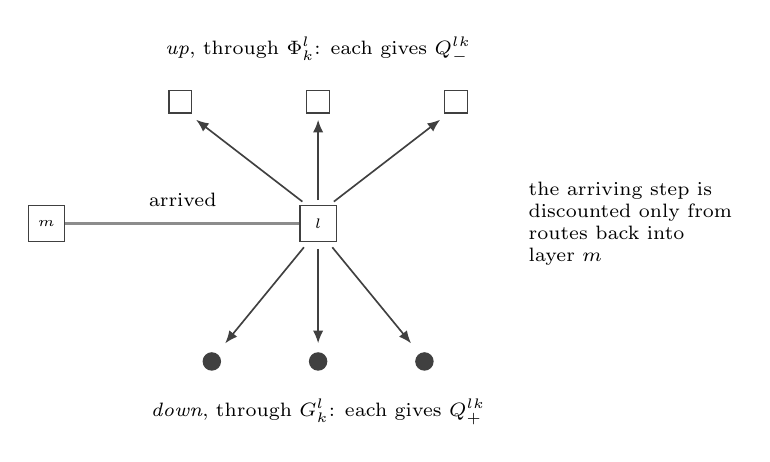
\begin{tikzpicture}
% the complex under consideration; layers are named inside the boxes so that no
% label has to compete with the arrows for space
\node[cpx,minimum size=4.6mm,font=\tiny] (E) at (0,0) {$l$};
% up: the complexes that include it
\node[cpx] (u1) at (-1.75,1.55) {}; \node[cpx] (u2) at (0,1.55) {};
\node[cpx] (u3) at (1.75,1.55) {};
\draw[msg] (-0.20,0.28) -- (-1.55,1.32);
\draw[msg] (0,0.30) -- (0,1.32);
\draw[msg] (0.20,0.28) -- (1.55,1.32);
\node[lb,anchor=south,align=center] at (0,1.92)
  {\emph{up}, through $\Phi^{l}_{k}$: each gives $Q^{lk}_{-}$};
% down: the complexes inside it
\node[atm] (d1) at (-1.35,-1.75) {}; \node[atm] (d2) at (0,-1.75) {};
\node[atm] (d3) at (1.35,-1.75) {};
\draw[msg] (-0.18,-0.30) -- (-1.18,-1.52);
\draw[msg] (0,-0.32) -- (0,-1.52);
\draw[msg] (0.18,-0.30) -- (1.18,-1.52);
\node[lb,anchor=north,align=center] at (0,-2.10)
  {\emph{down}, through $G^{l}_{k}$: each gives $Q^{lk}_{+}$};
% the arrival, and what it excludes
\node[cpx,minimum size=4.6mm,font=\tiny] (arr) at (-3.45,0) {$m$};
\draw[lnk,line width=1.1pt] (arr)--(E);
\node[lb,anchor=south] at (-1.72,0.10) {arrived};
\node[lb,anchor=west,align=left] at (2.55,0)
  {the arriving step is\\ discounted only from\\ routes back into\\ layer $m$};
\end{tikzpicture}
\end{adjustbox}
\caption{\textbf{The map.} A complex reached from layer $m$ fails to reach the
giant component only if every onward route fails --- every complex that includes
it and every complex inside it. Equations~\eqref{eq:Qminus}
and~\eqref{eq:Qplus} are that statement, one for each direction of arrival. The
only subtlety is the one on the right: the inclusion used to arrive must not be
counted again, but it was only ever a route back into layer $m$, so the excess
generating function is used for that layer and the ordinary one for every other.}
\label{fig:themap}
\end{figure}

Solving Eqs.~\eqref{eq:Qminus}--\eqref{eq:Qplus} --- by iteration from
$Q\equiv0$, which converges to the relevant fixed point --- gives everything.
The probability that a randomly chosen layer-$l$ complex is in no giant
component is the same statement made at a complex rather than along an
inclusion, so with no excess anywhere,
\begin{equation}
  P^{l}=\prod_{k}\Phi^{l}_{k}\bigl(Q^{lk}_{-}\bigr)
        \prod_{k}G^{l}_{k}\bigl(Q^{lk}_{+}\bigr),
  \qquad S_{l}=1-P^{l}.
  \label{eq:Sl}
\end{equation}

\paragraph{Occupation probabilities.} Site and bond occupation enter by
\emph{thinning} the generating functions rather than as a separate calculation:
a complex present with probability $p$ sends $\Phi\to1-p+p\Phi$. This makes
$S_{l}$ the fraction of \emph{all} layer-$l$ complexes rather than of surviving
ones, so that $S\le p$ automatically.

Thinning is not always the right move, and Chapter~\ref{ch:giant} turns on the
exception. When the connectivity rule already
implies that a complex is present --- as under AND-logic, where a hyperedge
functions only if all its members do --- a complex reached along a working
inclusion is present by construction, and folding the occupation probability
into the map would count it twice. It is then reinstated at the root only,
$P^{l}\to1-\pi_{l}+\pi_{l}P^{l}$.

\section{The threshold}
\label{sec:threshold}
\index{threshold tensor|textbf}

The map always has the trivial fixed point $Q\equiv1$: nothing is connected to
anything. A giant component exists exactly when that fixed point is unstable,
which is the chygraph version of the branching argument of
Sec.~\ref{sec:percolation-intro} --- one branch begetting more than one branch.

Linearising Eqs.~\eqref{eq:Qminus}--\eqref{eq:Qplus} about $Q\equiv1$ replaces
every generating function by its first derivative there, which by
Eq.~\eqref{eq:moments} is one of the four moment matrices $\ave{\kappa}$,
$\ave{\kbar}$, $\ave{s}$, $\ave{\sbar}$. The result is a linear operator on the
$2L^{2}$ unknowns --- the tensor $A$ of \citet{vazquez2023pre} --- and the
transition is where the largest eigenvalue of $-A$ passes through zero. The
sign is not cosmetic. Section~\ref{sec:jacobian} will show that $A$ is the
identity minus the Jacobian of the map, so its eigenvalues are the Jacobian's
subtracted from one, and the one that crosses zero at the transition is the
smallest of them rather than the largest.

Doing that expansion is what produces the blocks. Write $Q=1-\epsilon$. Every
generating function equals one at $Q\equiv1$, so a product of them is one at
zeroth order and each factor contributes nothing but its own first derivative,
\[
  \prod_{k}\Phi^{l}_{k}\bigl(1-\epsilon^{lk}_{-}\bigr)
    =1-\sum_{k}\ave{\kappa}_{lk}\,\epsilon^{lk}_{-}+O(\epsilon^{2}),
\]
and the same for $\bar\Phi$, $G$ and $\bar G$ with $\ave{\kbar}$, $\ave{s}$ and
$\ave{\sbar}$. The two products in each of Eqs.~\eqref{eq:Qminus}
and~\eqref{eq:Qplus} multiply, and to first order their corrections simply add,
so each equation becomes one row reading $\epsilon^{ml}_{\pm}$ against a sum of
moments times $\epsilon^{lk}_{-}$ and $\epsilon^{lk}_{+}$. Collecting every term
on one side gives $A\epsilon=0$, the identity piece below being the left-hand
side of that row and the moments what it is set equal to.

Index the four blocks of $A$ by the direction of arrival at the complex and the
direction of departure from it. With $\delta$ the Kronecker delta,
\begin{align*}
  (A_{--})^{ml}_{nk}&=\delta_{mn}\delta_{lk}-\ave{\kappa}_{nk}\delta_{nl},\\
  (A_{-+})^{ml}_{nk}&=-\bigl[\ave{\sbar}_{nk}\delta_{mk}
                      +\ave{s}_{nk}(1-\delta_{mk})\bigr]\delta_{nl},\\
  (A_{+-})^{ml}_{nk}&=-\bigl[\ave{\kbar}_{nk}\delta_{mk}
                      +\ave{\kappa}_{nk}(1-\delta_{mk})\bigr]\delta_{nl},\\
  (A_{++})^{ml}_{nk}&=\delta_{mn}\delta_{lk}-\ave{s}_{nk}\delta_{nl}.
\end{align*}
Every term carries $\delta_{nl}$ because three layers are in play at once: the
one come from ($m$), the one stood at ($l$), and the one gone to ($k$). The
$\delta_{mk}$ inside two of the blocks is Fig.~\ref{fig:themap}'s bracket again
--- the excess average when returning to the layer of origin, the ordinary
average otherwise.

Flatten the four blocks into one matrix by the vectorisation
$(\mathrm{vec}\,A)_{mL+l,\,nL+k}=A^{ml}_{nk}$,
\[
  \mathrm{vec}^{2}A=
  \begin{bmatrix}
    \mathrm{vec}(A_{--}) & \mathrm{vec}(A_{-+})\\
    \mathrm{vec}(A_{+-}) & \mathrm{vec}(A_{++})
  \end{bmatrix},
\]
and the distance above threshold is the largest eigenvalue of its negative,
\[
  \Lambda=\max_{\lambda}\ \mathrm{eigenvals}\bigl(-\mathrm{vec}^{2}A\bigr).
\]
Finite components when $\Lambda<0$, a giant component when $\Lambda>0$. The
order parameter is $S$, and Chapter~\ref{ch:giant} obtains it from $\Lambda$ by
carrying the same expansion one order further.

Since $\Lambda=0$ implies $\det(\mathrm{vec}^{2}A)=0$, it is often easier to work
with the \emph{pseudo-order parameter}
\[
  \theta=-\det\bigl(\mathrm{vec}^{2}A\bigr),
\]
which is a polynomial in the moments and usually has a far shorter closed form
than $\Lambda$. One warning: $\theta$ vanishes where
$\Lambda$ does, but the \emph{sign} of $\theta$ does not determine the phase. A
determinant vanishes whenever any eigenvalue does, not only the largest. Use
$\theta$ to locate the transition and $\Lambda$ to say which side of it the
system is on. The tensor is \code{giant.\allowbreak Chygraph.\allowbreak A} and the determinant \code{giant.\allowbreak Chygraph.\allowbreak theta}, both symbolic.

Two features of the tensor decide how it is used.

The tensor is built \emph{only} from the four first-moment matrices. Whatever
the cardinality of the complexes, whatever the depth of the inclusion hierarchy,
the threshold depends on the ensemble through four $L\times L$ matrices and
nothing else --- and $L$ is the number of layers, typically two or three. What
those four matrices fail to determine is the subject of Chapter~\ref{ch:giant},
and it is everything about the transition except where it is.

And the whole of it is symbolic. Once the matrices are written down, $\theta$
and $\Lambda$ come out of a computer algebra system with no further thought.
That is the sense in which the calculations below are substitutions rather than
derivations.

\section{Structure by structure}
\label{sec:structurebystructure}
\index{percolation!structure by structure}

Each of the following is one published result, obtained by writing the four
matrices for the structure of Sec.~\ref{sec:everything} and substituting.

\paragraph{Hypergraphs.} Layer $0$ the nodes, layer $1$ the hyperedges, present
with probabilities $p$ and $q$. The only non-zero entries are
$\ave{\kappa}_{01}=p\ave{k}$, $\ave{\kbar}_{01}=p\ave{\bar k}$,
$\ave{s}_{10}=q\ave{c}$, $\ave{\sbar}_{10}=q\ave{\bar c}$, and the result is
\begin{equation}
  \theta_{H}=pq\,\ave{\bar k}\ave{\bar c}-1,
  \qquad
  \Lambda_{H}=\sqrt{\theta_{H}+1}-1,
  \label{eq:thetaH}
\end{equation}
a giant component when $\theta_{H}\ge0$. This is the branching argument in its
plainest form: arriving at a node one can reach $\ave{\bar k}$ further
hyperedges, each of which offers $\ave{\bar c}$ further nodes, and the product
must exceed one. It agrees with the hypergraph percolation literature
\citep{coutinho2020,sun2021,bianconi2023}.

\paragraph{Graphs.} The same with cardinality fixed at two, so
$\ave{s}_{10}=2q$ and $\ave{\sbar}_{10}=q$:
\begin{equation}
  \theta_{G}=pq\,\ave{\bar k}-1.
  \label{eq:thetaG}
\end{equation}
For $p=q=1$ this is \citet{molloy1995}; for general $p$ and $q$
it is \citet{callaway2000}. It is also
Eq.~\eqref{eq:molloyreed}: the machinery reproduces
Chapter~\ref{ch:introduction} exactly.

\paragraph{Multiplex networks.} One node layer and $L$ link-type layers, with
$\ave{\kappa}_{0l}=p\ave{k}_{l}$ and so on for each $l$. For arbitrary degree
and cardinality distributions $\theta$ is a long polynomial, best left to the
computer. For Poisson distributions, where $\ave{x(x-1)}/\ave{x}=\ave{x}$ and
every excess average collapses to an ordinary one, it becomes
\begin{equation}
  \theta_{MP}=p\sum_{l=1}^{L}q_{l}\ave{k}_{l}\ave{c}_{l}-1,
  \label{eq:thetaMP}
\end{equation}
recovering \citet{sun2021}. The contribution of the layers is
\emph{additive}, and the comparison between the two cases identifies what makes
the general expression long: it is the excess averages, and nothing else.

\paragraph{Interacting graphs and hypergraphs.} Two hypergraphs plus a layer of
hyperedges containing nodes of both is a five-layer chygraph, and $g$
interacting hypergraphs with pairwise interaction layers need
$g+\binom{g+1}{2}$ layers under the indexing of
\citet{vazquez2024comnet}. The matrices are sparse and the substitution is
mechanical. Nothing further is required: interacting
networks needed their own literature \citep{leicht2009,bianconi2017}, and here
they are a choice of layer indices.

\paragraph{Network motifs, where the interior starts to matter.} Now a case that
is different, and the second half of the book depends on it. Give a graph a layer of plain links ($c=2$) and a layer of triangles
($c=3$), as in Sec.~\ref{sec:everything}, and ask about \emph{bond}
percolation --- links present with probability $q$.

A hyperedge either survives or does not. A triangle is not so simple: it has
three links, and how much of it one can reach depends on which of them survived
and which corner one came in by. This is the fine-grained interior of
Sec.~\ref{sec:definition} doing real work, and it means the intra-complex
component size $s$ is a random variable that has to be computed.

Arrive at corner $A$; call the others $B$ and $C$; the three links are present
independently with probability $q$. Enumerate the eight configurations and count
how many of $\{B,C\}$ are reachable from $A$.

Both are reachable if $AB$ and $AC$ are present, or if one of them is present
and $BC$ closes the path:
\[
  \Pr[\bar s=2]=q^{2}+2q(1-q)\,q=q^{2}(3-2q).
\]
Exactly one is reachable when its own link is present and both others are
absent, which can happen two ways:
\[
  \Pr[\bar s=1]=2q(1-q)^{2}.
\]
Neither is reachable when both of $A$'s links are absent, whatever $BC$ does:
$\Pr[\bar s=0]=(1-q)^{2}$. The three sum to one. The mean is
\[
  \bar s_{\triangle}(q)=2q^{2}(3-2q)+2q(1-q)^{2}
                       =2q\bigl(1+q-q^{2}\bigr),
\]
against $\bar s_{|}(q)=q$ for a plain link. At $q=1$ the triangle gives $2$ and
the link gives $1$, as they must. \code{figs/\allowbreak triangles\_\allowbreak vs\_\allowbreak regular.\allowbreak py} recomputes $\bar s_{\triangle}(q)$ by exact enumeration over the eight configurations, which is the check that the count above is right.

With those in hand the threshold follows as before. For a general graph with
links and triangles,
\begin{equation}
  \theta_{NM}=\sum_{l=|,\triangle}\bar s_{l}(q)\ave{\bar k}_{l}-1
    +\bar s_{|}\bar s_{\triangle}
     \bigl(\ave{k}_{|}\ave{k}_{\triangle}
          -\ave{\bar k}_{|}\ave{\bar k}_{\triangle}\bigr),
  \label{eq:thetaNM}
\end{equation}
the last term vanishing whenever the two layers are Poisson, in which case the
contributions are again additive. Setting the triangle layer to zero recovers
Eq.~\eqref{eq:thetaG}, as it must.

\section{Do triangles help or hurt?}
\label{sec:helporhurt}
\index{clustering!and percolation}
\index{null model}

Equation~\eqref{eq:thetaNM} raises an obvious question, and the published
answer \citep{vazquez2024comnet} appears to conflict with a result this book
reaches later. This section resolves the conflict.

Take two Poisson networks with the same total number of links, one with
triangles and one without. Since a node's degree gets $2$ from every triangle it
belongs to and $1$ from every plain link, the network with triangle parameters
$(\ave{k}_{|},\ave{k}_{\triangle})$ has the same link count as the
triangle-free network with $(\ave{k}_{|}+2\ave{k}_{\triangle},0)$. Then
\begin{equation}
  \theta_{P}\bigl(\ave{k}_{|},\ave{k}_{\triangle}\bigr)
  -\theta_{P}\bigl(\ave{k}_{|}+2\ave{k}_{\triangle},0\bigr)
  =2q^{2}(1-q)\,\ave{k}_{\triangle}\;>\;0,
  \label{eq:deltatheta}
\end{equation}
so at equal link count the clustered network percolates more easily and, since
an epidemic is a bond percolation problem (Chapter~\ref{ch:epidemics}), spreads
infection more easily too. This agrees with \citet{newman2003}.

Chapter~\ref{ch:ising} reaches the opposite conclusion for the Ising model: at
fixed degree distribution, clustering \emph{lowers} the critical temperature, by
$13.9$ per cent for two triangles per vertex against the $4$-regular graph.
Ordering is harder, not easier. Both results are correct, and the reason they
point in opposite directions is that they are not the same comparison.

Equation~\eqref{eq:deltatheta} holds the number of links fixed. It does not hold
the \emph{degree distribution} fixed, and it is easy to see why not. A triangle
hands a node two links at once, so the degree of a node in the clustered network
is a sum with a factor of two in it, and its variance is inflated: with Poisson
counts, $\mathrm{Var}[k]=\ave{k}_{|}+4\ave{k}_{\triangle}$ against a mean of
$\ave{k}_{|}+2\ave{k}_{\triangle}$. Working through Eq.~\eqref{eq:excessdeg},
the clustered network's excess degree exceeds the control's by
$2\ave{k}_{\triangle}/(\ave{k}_{|}+2\ave{k}_{\triangle})$. It is not less
clustered, but it \emph{is} more heterogeneous, and
Sec.~\ref{sec:percolation-intro} showed that heterogeneity is what lowers a
percolation threshold. Equation~\eqref{eq:deltatheta} is measuring that.

This is the caution of Sec.~\ref{sec:promoting} in a new place. There, a
degree-matched control turned out to manufacture clustering; here, a
link-matched control turns out to remove degree heterogeneity. In both cases the
lesson is the same: name what is held fixed before reading a comparison as a
statement about clustering.

So hold the degree fixed instead, which is possible exactly and with no
distributional freedom left. A network in which every node belongs to exactly
two triangles has degree $4$ at every node and $2n$ links. So does the
$4$-regular random graph. They differ in clustering --- $1/3$ against $0$ ---
and in nothing else that Chapter~\ref{ch:introduction} can see. For the
$4$-regular graph $\ave{\bar k}=3$ and Eq.~\eqref{eq:thetaG} gives
$\theta=3q-1$. For the triangle network the chy-degree is $2$, its excess is
$1$, and Eq.~\eqref{eq:thetaNM} gives $\theta=\bar s_{\triangle}(q)-1$. Hence
\begin{equation}
  \begin{aligned}
    q_{c}&=\tfrac13=0.3333,\\
    2q_{c}\bigl(1+q_{c}-q_{c}^{2}\bigr)&=1,\quad q_{c}=0.4030.
  \end{aligned}
  \label{eq:qc}
\end{equation}
Putting the same links into triangles raises the percolation threshold by $20.9$
per cent. Figure~\ref{fig:triangles} confirms it by Monte Carlo on both
structures at $n=3\times10^{4}$: the giant components lift off exactly where
Eq.~\eqref{eq:qc} says.

\begin{figure}[t]
\centering
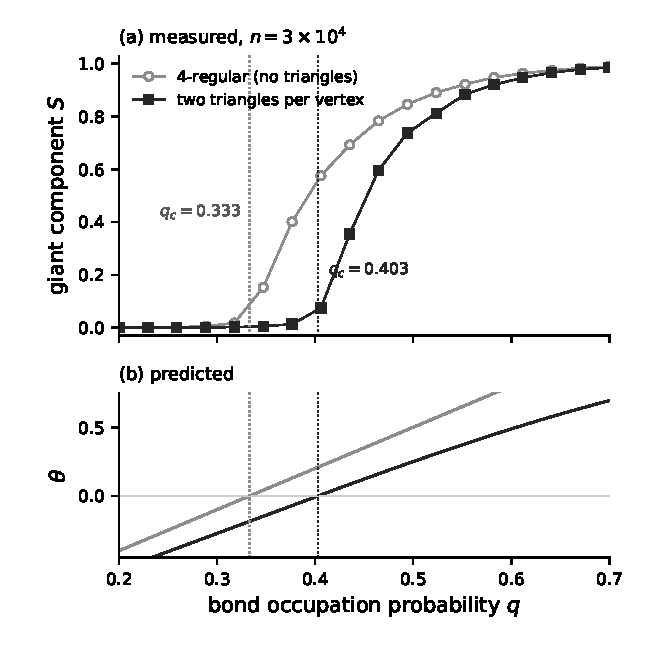
\includegraphics[width=0.86\linewidth]{figs/fig-triangles.pdf}
\caption{\textbf{Triangles hurt, at fixed degree.} Two networks with degree $4$
at every node and the same number of links; the only difference is that one has
its links arranged in triangles, giving clustering $1/3$ against $0$. (a) The
giant component measured by Monte Carlo. (b) The prediction, $\theta=3q-1$ and
$\theta=\bar s_{\triangle}(q)-1$. The measured onsets sit on the predicted
thresholds. Compare Eq.~\eqref{eq:deltatheta}, which finds the opposite sign at
fixed \emph{link count} --- because that comparison lets the degree distribution
broaden. Generated by \code{figs/\allowbreak triangles\_\allowbreak vs\_\allowbreak regular.\allowbreak py}.}
\label{fig:triangles}
\end{figure}

The mechanism is the one Chapter~\ref{ch:ising} will give for the Ising model,
in the form that covers both. A triangle transmits
\emph{more per neighbour} than a link does: at $q=1$ it delivers two nodes where
a link delivers one, and Eq.~\eqref{eq:thetaNM}'s $\bar s_{\triangle}$ exceeds
$\bar s_{|}$ at every $q$. But a node of degree four spends its four links on
two triangles rather than on four independent links, so it has \emph{two}
branches to explore instead of four. More per branch, fewer branches --- and the
second effect is the larger. That sentence, with $\bar s$ replaced by the
transmission of a magnetisation, is Chapter~\ref{ch:ising}'s headline result.

\section{Checks}
\label{sec:percolation-checks}

\checkhead{Known results}
Every specialisation in Sec.~\ref{sec:structurebystructure} reproduces a
published formula --- Molloy--Reed, Callaway \emph{et al.}, the hypergraph
result, \citeauthor{sun2021}'s multiplex expression. This tests the algebra and
nothing else.

\checkhead{New results}
Section~\ref{sec:helporhurt} is the only part of the chapter with no published
counterpart. Its two thresholds, $q_{c}=1/3$ for the $4$-regular graph and
$q_{c}=0.4030$ for the network of triangles, are confirmed by Monte Carlo on
both structures at $n=3\times10^{4}$ (Fig.~\ref{fig:triangles}): the measured
onsets sit on the predicted thresholds.

\checkhead{Partial results}
Sampling a chygraph from the configuration-model construction of
Sec.~\ref{sec:sampling} and percolating it tests the map, and not the assumption
the map rests on, because a chygraph built that way has complexes meeting in at
most one atom by construction. Figure~\ref{fig:triangles} is halfway past that:
the two-triangles-per-vertex network is a real graph, but it too was built with
the triangles sharing at most one atom. Nothing in this chapter needed the
complexes to be small, or the layers to be few, or the cardinality distribution
to be narrow; what it needed was that single assumption, and no check here tests
it. Building a structure where complexes share more is
Chapter~\ref{ch:overlap}'s business, and there the theory is not exact.


% sources
% - manuscript 1, Secs. III-IV (with and without intra-layer inclusions)
% - manuscript 2, Secs. 3-6 (order parameter, graphs/hypergraphs, multiplex,
%   interacting graphs and hypergraphs)

\chapter{Beyond the threshold}
\label{ch:giant}

Chapter~\ref{ch:percolation} located the threshold but said nothing about the
size of the giant component. The tensor $A$ is built from four matrices of first
moments; the map needs whole generating functions. The threshold therefore uses
strictly less information than the map, and in this chapter we ask what the
rest of that information buys. The results are reported here for the first
time; where they extend the percolation map of
\citet{vazquez2023pre,vazquez2024comnet} the debt is marked at the point of use.

What it buys is a hierarchy, Table~\ref{tab:hierarchy}, and an unusually clean
one: each additional order of moment data buys exactly one more thing about the
transition.

\begin{table}[b]
\centering\small
\begin{tabular}{ll}
\hline\hline
quantity & input required\\
\hline
threshold $\theta$, $\Lambda$ & first moments\\
critical amplitude $B$ & $+$ second moments\\
$S$ away from the threshold & the generating functions\\
\hline\hline
\end{tabular}
\caption{\textbf{What each level of input determines.} The threshold needs the
four moment matrices of Sec.~\ref{sec:ensembles} and nothing else. One further
order of moments fixes the slope with which the giant component grows out of
the threshold. Nothing short of the full distributions fixes its size away from
there.}
\label{tab:hierarchy}
\end{table}

Establishing the hierarchy needs one structural observation, made in
Sec.~\ref{sec:jacobian}, and everything else follows from it. This chapter also
lifts an assumption that has been in force since Sec.~\ref{sec:ensembles} ---
that a complex's participation in one layer says nothing about its
participation in another --- and shows that lifting it matters more than one
might expect.

\section{The threshold is a Jacobian}
\label{sec:jacobian}
\index{threshold tensor}
\index{Jacobian}

Differentiate the map, Eqs.~\eqref{eq:Qminus}--\eqref{eq:Qplus}, at the trivial
fixed point $Q\equiv1$. Every generating function equals one there, so each
product leaves a single first derivative, and by Eq.~\eqref{eq:moments} each of
those is an entry of one of the four moment matrices. Comparing the result with
the tensor of Sec.~\ref{sec:threshold} entry by entry gives
\begin{equation}
  \mathrm{vec}^{2}A=I-J,
  \qquad
  J_{ab}=\frac{\partial F_{a}}{\partial Q_{b}}\bigg|_{Q=1},
  \label{eq:AisJ}
\end{equation}
where $F$ is the map. The published threshold tensor \emph{is} the Jacobian of
the map at its trivial fixed point. Consequently
\begin{equation}
  \Lambda=\lambda-1,
  \label{eq:Lambdalambda}
\end{equation}
with $\lambda$ the Perron root of $J$: the threshold calculation is the
statement that $Q\equiv1$ loses stability, exactly as
Sec.~\ref{sec:percolation-intro} said it should be.

The four blocks of $A$ acquire a plain reading from this. They are the four ways
of composing a step with the state it lands in --- up then up, up then down,
down then up, down then down --- and the Kronecker deltas $\delta_{mk}$ that
select the excess averages are precisely the brackets $[\,\cdot\,]_{k=m}$ of
Fig.~\ref{fig:themap}, which is to say the rule that the arriving inclusion is
discounted only from routes back into the layer it came from. Nothing in $A$ was
ever arbitrary.

The observation is small and it carries the chapter: threshold and order
parameter are not two calculations but two orders of one, on the same index set and in the same layout. Everything in this chapter is
obtained by carrying that expansion further or by changing what is expanded.

\section{What the first moments do not determine}
\label{sec:degeneracy}
\index{null model}

Since $A$ depends on the ensemble only through first moments, and moments do not
determine a distribution, $S$ cannot be a function of $A$. The size of the
degeneracy is measured below.

Take two graphs whose degree distributions are
\begin{align}
  P_{A}(k)&=0.5\,\delta_{k,0}+0.5\,\delta_{k,4},\nonumber\\
  P_{B}(k)&=0.2\,\delta_{k,0}+0.5\,\delta_{k,1}+0.3\,\delta_{k,5}.
  \label{eq:PAPB}
\end{align}
Both have $\ave{k}=2$ and $\ave{\bar k}=3$. They therefore have identical
$\theta=3p-1$, identical $\Lambda$, and the identical site percolation threshold
$p_{c}=1/3$ --- every entry of the threshold tensor agrees. At $p=1$ the first
has $S=0.500$ and the second $S=0.673$ (Fig.~\ref{fig:degeneracy}). Nothing in
Chapter~\ref{ch:percolation} can tell them apart, and they differ by a third.

\begin{figure}[t]
\centering
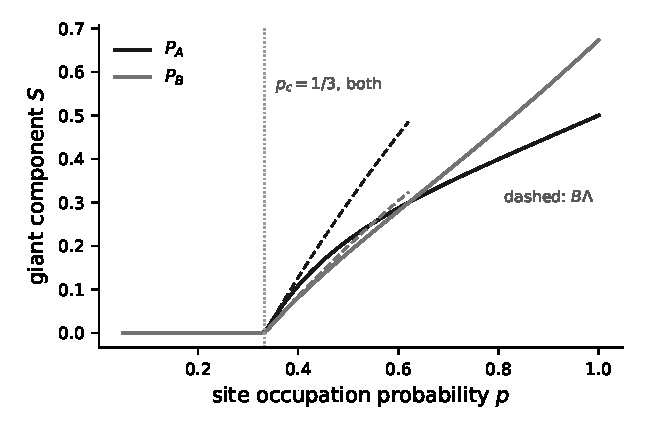
\includegraphics[width=0.9\linewidth]{figs/fig-degeneracy.pdf}
\caption{\textbf{First moments do not determine the order parameter.} Site
percolation on two configuration-model graphs with the degree distributions of
Eq.~\eqref{eq:PAPB}, which share $\ave{k}=2$ and $\ave{\bar k}=3$ and hence
share every entry of the threshold tensor. They share the threshold $p_{c}=1/3$
and nothing else: the order parameter differs everywhere above it, and so does
the slope with which it leaves. Dashed lines are the leading behaviour
$B\Lambda$ of Eq.~\eqref{eq:Bgraph}, $B=4/3$ and $B=8/9$. Generated by
\code{figs/\allowbreak beyond\_\allowbreak threshold.\allowbreak py}.}
\label{fig:degeneracy}
\end{figure}

The extra input is nonetheless cheap, and this is the practical point. Every
example in Chapter~\ref{ch:percolation} was built from a distribution and then
projected onto its mean. The bond-percolated triangle is the clearest case: the
enumeration in Sec.~\ref{sec:structurebystructure} produced a whole
distribution over excess component sizes, of which $\bar
s_{\triangle}(q)=2q(1+q-q^{2})$ was only the mean. Written as a generating
function it is
\begin{equation}
  \begin{aligned}
    \bar G_{\triangle}(y)&=\bigl(3q^{2}-2q^{3}\bigr)y^{2}+2q(1-q)^{2}y\\
    &\quad+(1-q)^{3}+q(1-q)^{2}.
  \end{aligned}
  \label{eq:tripgf}
\end{equation}
Un-projecting is a one-line change per model. And for Poisson distributions
there is nothing to un-project, since $\Phi=\bar\Phi=e^{\ave{\kappa}(x-1)}$ is
already fixed by its mean.

\citet{vazquez2024comnet} gives the mean intra-complex component size
of a triangle --- as opposed to the \emph{excess} size, which is what the
threshold uses --- with $3/2$ on the single-link term. It should be $5/3$: in the configuration
with one bond present the three members sit in components of sizes $2$, $2$
and $1$, so a member chosen at random is in a component of mean size
$(2+2+1)/3=5/3$, not $3/2$. Weighting each configuration by its probability,
\begin{align*}
  s_{\triangle}(q)&=3\bigl[q^{3}+3q^{2}(1-q)\bigr]
    +\tfrac{5}{3}\bigl[3q(1-q)^{2}\bigr]+1\cdot(1-q)^{3}\\
  &=3\bigl(q^{3}+3q^{2}(1-q)\bigr)+5q(1-q)^{2}+(1-q)^{3},
\end{align*}
the $5/3$ and the $3$ multiplying out to the $5$ in the collapsed form. That
is $s_{\triangle}=1+\bar s_{\triangle}=1+2q(1+q-q^{2})$, which is what
Eq.~\eqref{eq:tripgf} returns.

The published threshold is unaffected, for a definite reason:
$\ave{s}_{20}$ never enters $\theta$ at all, because triangles are never reached
from above --- nothing includes a triangle. The coefficient does enter the order
parameter of the triangle layer, $S_{2}$. Both forms are in \code{figs/\allowbreak triangles\_\allowbreak vs\_\allowbreak regular.\allowbreak py}, which enumerates the triangle rather than quoting it.

\section{The critical amplitude}
\label{sec:amplitude}
\index{critical amplitude|textbf}
\index{order parameter}

Between ``first moments'' and ``the whole distribution'' there is one more rung,
and it is reached by carrying the expansion of Sec.~\ref{sec:jacobian} to second
order.

Write $Q=1-x$ and expand the map about the trivial fixed point,
\[
  x_{a}=\sum_{b}J_{ab}x_{b}-\tfrac12\sum_{bc}M_{abc}x_{b}x_{c}+O(x^{3}),
\]
with $M_{abc}=\partial^{2}F_{a}/\partial Q_{b}\partial Q_{c}$ at $Q=1$. Let $r$
and $\ell$ be the right and left Perron vectors of $J$, normalised so that
$\ell\cdot r=1$. Just above threshold $\lambda=1+\Lambda$ with
$\Lambda\to0^{+}$; putting $x=\epsilon r$ and projecting on $\ell$ annihilates
the linear term and leaves
\[
  \epsilon=\frac{2\Lambda}{C},\qquad C\equiv\ell\cdot M[r,r].
\]
Expanding Eq.~\eqref{eq:Sl} to first order then gives
\[
  S_{l}=B_{l}\Lambda+O(\Lambda^{2}),
  \qquad
  B_{l}=\frac{2\,\nabla P^{l}\cdot r}{C}.
\]
Only \emph{second} derivatives of the generating functions enter $B_{l}$: one
moment order beyond what $A$ needs, and no more. That is the middle row of
Table~\ref{tab:hierarchy}.

Two things make this practical rather than merely formal. The rank-three tensor
$M$ never has to be built, since contracting it twice with $r$ is a second
directional derivative, $M_{a}[r,r]=\frac{d^{2}}{dt^{2}}F_{a}(1+tr)|_{t=0}$ ---
an ordinary single-variable derivative of a product of generating functions. And
the $2L^{2}$ indices collapse: discarding iteratively every index whose row or
column of $J$ vanishes identically leaves a \emph{core} without changing the
non-zero spectrum. For a hypergraph that is $2$ indices of $8$; for a graph with
links and triangles, $4$ of $18$. In both cases the survivors are exactly the
unknowns one would have written down by hand. \code{amplitude.\allowbreak CriticalAmplitude} carries this: the directional derivative, the core reduction, and $B_{l}$.

Table~\ref{tab:amplitudes} collects the closed forms on the critical manifold.
The graph is worth doing by hand, because there the two indices collapse to the
single scalar of Sec.~\ref{sec:percolation-intro} and the whole of the recipe
above fits in four lines. Write $x=1-u$ for the probability that a link does
lead to the giant component. Then $u=1-pq+pq\,G_{1}(u)$ is
\[
  x=pq\Bigl[\ave{\bar k}\,x-\tfrac12\ave{\bar k(\bar k-1)}\,x^{2}\Bigr]
    +O(x^{3}),
\]
since $G_{1}(1-x)=1-\ave{\bar k}x+\tfrac12\ave{\bar k(\bar k-1)}x^{2}-\cdots$.
Dividing by $x$ and solving,
\[
  x=\frac{2\bigl(pq\ave{\bar k}-1\bigr)}{pq\ave{\bar k(\bar k-1)}}.
\]
The Perron root here is $\lambda=\sqrt{pq\ave{\bar k}}$ --- a square root
because a graph is two layers and the Jacobian carries the product across them
--- so $pq\ave{\bar k}=(1+\Lambda)^{2}$ and the bracket is $2\Lambda$ to leading
order. Finally $S=p\bigl[1-G_{0}(1-x)\bigr]\simeq p\ave{k}\,x$, and on the
critical manifold $pq\ave{\bar k}=1$, so
\begin{equation}
  \lambda=\sqrt{pq\ave{\bar k}},
  \qquad
  B=\frac{4p\,\ave{k}\ave{\bar k}}{\ave{\bar k(\bar k-1)}}.
  \label{eq:Bgraph}
\end{equation}
Only the second factorial moment of the excess degree entered, which is the
middle row of Table~\ref{tab:hierarchy} in the one case where it can be watched
happening. A Poisson degree distribution has
$\ave{\bar k(\bar k-1)}=\ave{k}^{2}$ and $\ave{\bar k}=\ave{k}$, giving $B=4p$,
the first row of Table~\ref{tab:amplitudes}.
The hypergraph goes the same way with one more generating function in the
chain, and for arbitrary degree and cardinality distributions it gives
\begin{equation}
  B=\frac{4p\,\ave{k}\ave{\bar k}\ave{\bar c}}
         {\ave{\bar c}\ave{\bar k(\bar k-1)}
          +p\ave{\bar k}^{2}\ave{\bar c(\bar c-1)}}.
  \label{eq:Bhyper}
\end{equation}
Equation~\eqref{eq:Bgraph} separates the two distributions of
Fig.~\ref{fig:degeneracy}: they agree on $\ave{k}$ and $\ave{\bar k}$ but have
$\ave{\bar k(\bar k-1)}=6$ and $9$, giving $B=4/3$ against $8/9$. Setting the
degree distribution Poisson gives $B=4p$, and at $p=q=1$ the
Erd\H{o}s--R\'enyi result $S\simeq2(\ave{k}-1)$.

\begin{table}[t]
\centering\small
\begin{adjustbox}{max width=\linewidth}
\begin{tabular}{lll}
\hline\hline
system & $\lambda$ & $B$\\
\hline
Poisson graph & $\sqrt{pq\ave{k}}$ & $4p$\\[2pt]
Poisson hypergraph & $\sqrt{pq\ave{k}\ave{c}}$ & $4p/(1+p\ave{c})$\\[2pt]
Poisson multiplex & $\bigl(\sum_{l}q_{l}\ave{k}_{l}\ave{c}_{l}\bigr)^{1/2}$
  & $4\big/\bigl(1+\sum_{l}q_{l}\ave{k}_{l}\ave{c}_{l}^{2}\bigr)$\\[2pt]
Poisson, triangles & $\bigl(q\ave{k}_{|}
  +2q(1{+}q{-}q^{2})\ave{k}_{\triangle}\bigr)^{1/2}$
  & $4\big/\bigl[1+2q^{2}(3-2q)\ave{k}_{\triangle}\bigr]$\\
\hline\hline
\end{tabular}
\end{adjustbox}
\caption{\textbf{Critical amplitudes} in $S=B\Lambda+O(\Lambda^{2})$, on the
critical manifold $\lambda=1$. Sites are present with probability $p$, bonds or
hyperedges with probability $q$. The arbitrary-distribution cases are
Eqs.~\eqref{eq:Bgraph} and~\eqref{eq:Bhyper}.}
\label{tab:amplitudes}
\end{table}

The last row of Table~\ref{tab:amplitudes} contains something the threshold
could not have shown. For bond percolation on a graph with links and triangles,
\begin{equation}
  B=\frac{4}{1+2q^{2}(3-2q)\ave{k}_{\triangle}},
  \label{eq:Btriangle}
\end{equation}
and $\ave{k}_{|}$ does not appear. The link layer moves the threshold but not
the amplitude. The reason is the fine-grained interior of
Sec.~\ref{sec:definition}: a link's excess component size is Bernoulli, its
generating function is affine, and an affine function has no second derivative
to contribute. At the level of $\theta$ the two layers enter symmetrically and
nothing suggests this. It is a distinction that only appears one order up.

\section{Where the expansion breaks down}
\label{sec:breakdown}
\index{interdependent networks|textbf}
\index{spinodal}

The denominator $C=\ell\cdot M[r,r]$ is a sum of non-negative terms, since
$\ell$, $r$ and all second derivatives of generating functions at $1$ are
non-negative. When it is finite and positive, the transition is continuous with
$S\propto\Lambda$ and order parameter exponent $\beta=1$. Both qualifications
carry weight.

\emph{$C$ can diverge.} Finiteness is a condition on second factorial moments of
the excess distributions --- again one order beyond $\theta$. For a graph
$C\propto\ave{\bar k(\bar k-1)}=\ave{k(k-1)(k-2)}/\ave{k}$, which diverges for a
scale-free degree distribution with exponent $\gamma\le4$. There
Eq.~\eqref{eq:Bgraph} returns $B\to0$: the linear branch has vanishing
amplitude, $\beta\ne1$, and one recovers the familiar $\beta=1/(\gamma-3)$ of
heterogeneous mean field for $3<\gamma<4$. The expansion announces its own
breakdown, but the closed forms of Table~\ref{tab:amplitudes} are statements about ensembles with finite second
moments and must not be quoted outside that range.

\emph{$C$ can vanish.} Then the map is affine along the critical direction and
there is no linear branch at all. The elementary case is the two-regular graph,
where $\bar\Phi(x)=x$ and there is no transition of this type. So $C$ is a
symbolic continuity criterion, computable alongside $\theta$ and $\Lambda$.

Its non-negativity settles something. It has recently been argued
\citep{keating2026} that group structure on its own produces only continuous
transitions. For anything in the percolation class this now has a one-line
proof: a complex contributes to $C$ through second derivatives of its
generating functions, and those cannot be negative. The qualifier \emph{on its
own} is doing work.
Section~\ref{sec:groupcontagion} maps a threshold rule to a chygraph and keeps
the recursion, but its intra-complex function is not a generating function in
the failure variable, and the onset can then be discontinuous.

One caveat delimits the scope, and it is an exclusion rather than a
technicality. Equations~\eqref{eq:Qminus}--\eqref{eq:Qplus} are the extinction
conditions of a multi-type branching process, and for such maps the loss of
stability of $Q\equiv1$ locates the transition. Interdependent networks
\citep{buldyrev2010,radicchi2015} are not of this class: their giant component
appears through a saddle-node bifurcation while $Q\equiv1$ is \emph{still
stable}, so $\Lambda=0$ does not locate the transition and the physical fixed
point has to be reached by a cascade from above rather than by iterating up from
$Q=0$. Mapping those constructions to chygraphs, and identifying what replaces
$\Lambda$ there, is not done.

\section{Dependent layers}
\label{sec:joint}
\index{correlated layers|textbf}

In this section we lift the factorisation assumption.
Section~\ref{sec:ensembles} took the generating functions to factorise over
target layers, $\Phi^{l}(x)=\prod_{k}\Phi^{l}_{k}(x_{k})$. That
covers every mapping in Chapter~\ref{ch:percolation}, and it is false for
anything in which a complex's participation in one layer is tied to its
participation in another: a node whose triangle count moves with its link count,
a hyperedge whose cardinalities in two vertex layers are correlated. Joint
degree distributions of exactly this kind are what the motif formalism of
\citet{mann2021} works with, and Chapter~\ref{ch:data} recommended
measuring the correlation rather than assuming it away.

Dropping the factorisation changes the \emph{status} of the excess generating
functions. They stop being independent inputs and become derivatives of the
joint one,
\begin{equation}
  \bar\Phi^{l,(m)}(x)=\frac{\partial\Phi^{l}/\partial x_{m}}
    {\left.\partial\Phi^{l}/\partial x_{m}\right|_{x=1}},
  \label{eq:excessderived}
\end{equation}
and likewise for $\bar G$. The map becomes
\begin{align}
  Q^{ml}_{-}&=\Phi^{l}\bigl(Q^{l\cdot}_{-}\bigr)\,
              \bar G^{l,(m)}\bigl(Q^{l\cdot}_{+}\bigr),\nonumber\\
  Q^{ml}_{+}&=\bar\Phi^{l,(m)}\bigl(Q^{l\cdot}_{-}\bigr)\,
              G^{l}\bigl(Q^{l\cdot}_{+}\bigr),
  \label{eq:jointmap}
\end{align}
reducing term by term to Eqs.~\eqref{eq:Qminus}--\eqref{eq:Qplus} when the
functions factorise.

Differentiating at $Q=1$, a second derivative of the joint function now stands
where the published tensor carried a first moment. Define the
\emph{inclusion-biased} moments
\begin{equation}
  \ave{\bar\kappa^{(m)}}_{lk}
   =\frac{\ave{\kappa_{lm}\bigl(\kappa_{lk}-\delta_{mk}\bigr)}}
         {\ave{\kappa_{lm}}},
  \label{eq:biased}
\end{equation}
and likewise $\ave{\bar s^{(m)}}$: the expected chy-degree to layer $k$ of a
complex \emph{reached through an inclusion into layer $m$}. That is the whole
generalisation. Unconditional first moments are replaced by inclusion-biased
second moments, and everything downstream --- the Jacobian, the determinant, the
fixed point --- is unchanged.

\subsection{Identical marginals, different transitions}

The correction is not small. The demonstration below holds the marginals fixed
exactly. Take bond percolation on a graph with links and triangles, and
three joint distributions of the number of links $k_{|}$ and triangles
$k_{\triangle}$ at a node, each with the marginals $k_{|}\in\{1,3\}$ and
$k_{\triangle}\in\{0,2\}$ with probability $1/2$:
\begin{align}
  \text{correlated:}&\quad(k_{|},k_{\triangle})\in\{(1,0),(3,2)\},\nonumber\\
  \text{anti-correlated:}&\quad(k_{|},k_{\triangle})\in\{(1,2),(3,0)\},\nonumber\\
  \text{independent:}&\quad\text{the product of the marginals.}
\end{align}
All three have $\ave{k}_{|}=2$, $\ave{\bar k}_{|}=3/2$,
$\ave{k}_{\triangle}=\ave{\bar k}_{\triangle}=1$, hence every entry of the
published threshold tensor agrees. Equation~\eqref{eq:biased} separates them
through $\ave{\bar\kappa^{(1)}}_{0\triangle}=\ave{k_{|}k_{\triangle}}/\ave{k_{|}}$,
which is $3/2$, $1/2$ and $1$ --- the last coinciding with
$\ave{\kappa}_{0\triangle}=1$, as it must. The three bond percolation thresholds
are
\begin{equation}
  q_{c}=0.1939,\qquad 0.3161,\qquad 0.2409,
  \label{eq:qc3}
\end{equation}
a spread of more than sixty per cent, and the order parameters differ everywhere
above them (Fig.~\ref{fig:correlated}). The first moments predict the middle
curve for all three.

\begin{figure}[t]
\centering
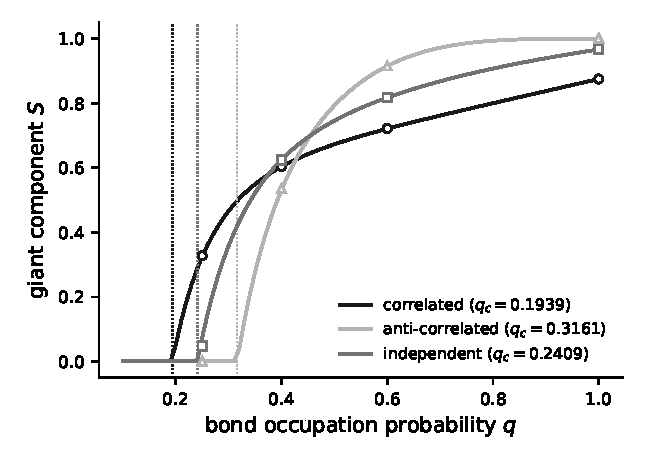
\includegraphics[width=0.9\linewidth]{figs/fig-correlated.pdf}
\caption{\textbf{Identical marginals, three transitions.} Bond percolation on a
graph with links and triangles, for three joint distributions of a node's link
and triangle counts sharing all marginals and therefore every entry of the
published threshold tensor. Lines are Eq.~\eqref{eq:jointmap}, symbols Monte
Carlo at $n=1.5\times10^{5}$, dotted lines the thresholds of
Eq.~\eqref{eq:qc3}. The curves cross between $q=0.38$ and $q=0.46$, so no single statement about
whether correlation helps survives. Generated by
\code{figs/\allowbreak beyond\_\allowbreak threshold.\allowbreak py}.}
\label{fig:correlated}
\end{figure}

The mechanism is intuitive once seen. Positive correlation piles both kinds of
connectivity onto the same nodes, which lowers the threshold --- those nodes
form a well-connected core --- but caps the reachable fraction, because the
complementary nodes are poorly connected in both layers at once.
Anti-correlation spreads connectivity out, raising the threshold but eventually
pulling everything in, $S\to1$ at $q=1$. Neither effect is visible in the first
moments.

\paragraph{One thing to check for.} The fixed point returns the fraction of
complexes in an \emph{infinite} component, which percolation theory identifies
with \emph{the} giant component on the assumption that the infinite component is
unique. Correlated layers can break that. If
$\Phi^{0}(x)=\tfrac12x_{|}^{2}+\tfrac12x_{\triangle}^{2}$ then no node
participates in both layers, the chygraph falls into two disjoint pieces, and
the map returns the sum of their infinite components rather than the larger: at
$q=1$ it reports $S=1$ where simulation gives $1/2$. The decomposition is easy
to test for, and it does not arise when some layer is supercritical on its own
and touches every complex.

\section{Constructions solved by substitution}
\label{sec:constructions}

The point of doing the work once is to be able to stop doing it. Each of the
following has been treated in the literature with a purpose-built calculation,
and each is handled here by writing down the chygraph and substituting.

\subsection{AND-logic against OR-logic}

\citet{bianconi2024} distinguish two rules for what a
higher-order interaction does when some of its members are removed. Under
\emph{OR}-logic the interaction keeps connecting whichever members survive.
Under \emph{AND}-logic it fails outright if any member is missing --- the right
rule for a chemical reaction, a catalytic step, a supply chain.
\citet{ha2025} reach the same distinction independently.

Both are the same chygraph: atoms in layer $0$, hyperedges in layer $1$. They
differ in one generating function,
\begin{equation}
  \bar G^{1}_{0}(y)=
  \begin{cases}
    \bar G_{c}(1-p+py), & \text{OR},\\[2pt]
    1-\bar G_{c}(p)+\bar G_{c}(py), & \text{AND}.
  \end{cases}
  \label{eq:andor}
\end{equation}
Neither $\Phi^{0}_{1}$ nor $\bar\Phi^{0}_{1}$ is thinned, because under either
rule a node reached along a functioning hyperedge is present by construction ---
this is the exception flagged in Sec.~\ref{sec:map}, and node occupation
reappears at the root alone. Nothing downstream knows which rule was chosen.

Differentiating Eq.~\eqref{eq:andor} at $y=1$ reduces the whole difference to
one substitution:
\begin{equation}
  \ave{\bar s}_{10}=p\,\bar G_{c}'(1)\ \text{ (OR)},
  \qquad
  \ave{\bar s}_{10}=p\,\bar G_{c}'(p)\ \text{ (AND)},
  \label{eq:andors}
\end{equation}
the same expression at $1$ and at $p$. Since $\bar G_{c}'$ is a power series
with non-negative coefficients it is non-decreasing on $[0,1]$, so
$\bar G_{c}'(p)\le\bar G_{c}'(1)$ and
\begin{equation}
  \theta_{\mathrm{AND}}\le\theta_{\mathrm{OR}},
  \qquad
  p_{c}^{\mathrm{AND}}\ge p_{c}^{\mathrm{OR}},
\end{equation}
with equality if and only if $p=1$ or $c\equiv2$ --- for an ordinary graph the
two rules are the same statement. That is a one-line proof of the inequality
reported by \citet{bianconi2024}. For Poisson degrees and cardinalities,
$\theta_{\mathrm{OR}}=p\ave{k}\ave{c}-1$ and
$\theta_{\mathrm{AND}}=p\ave{k}\ave{c}e^{\ave{c}(p-1)}-1$; at $\ave{k}=2$,
$\ave{c}=3$ the thresholds are $1/6$ and $0.5827$, more than a factor of three
apart (Fig.~\ref{fig:andor}).

\begin{figure}[t]
\centering
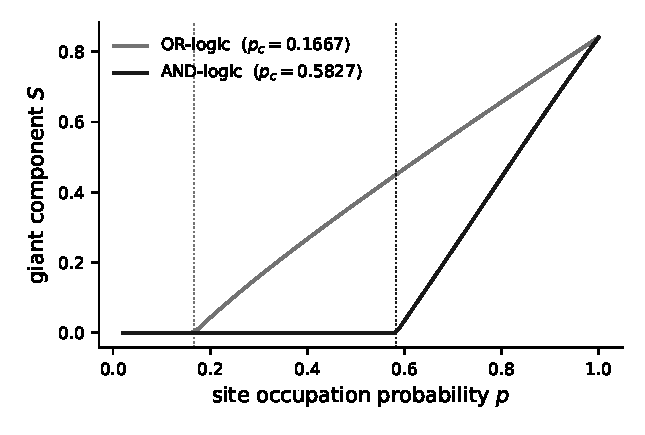
\includegraphics[width=0.9\linewidth]{figs/fig-andor.pdf}
\caption{\textbf{One chygraph, one generating function apart.} Site percolation
on a Poisson hypergraph, $\ave{k}=2$, $\ave{c}=3$, under the two rules of
Eq.~\eqref{eq:andor}: a hyperedge that keeps connecting its survivors, against
one that fails if any member is missing. The thresholds differ by a factor of
$3.5$; the curves must meet at $p=1$, where the rules coincide. Generated by
\code{figs/\allowbreak beyond\_\allowbreak threshold.\allowbreak py}.}
\label{fig:andor}
\end{figure}

\subsection{Hyperdegree--cardinality correlation}

Whether nodes of high hyperdegree join hyperedges of large cardinality is a
measurable property of real hypergraphs and one known to matter
\citep{ha2025,fujiki2018}. It is a correlation between layers in the sense of
Sec.~\ref{sec:joint}: split the hyperedges into layers by cardinality class, and
the joint chy-degree generating function \emph{is} the correlation.

Taking classes $c=2$ and $c=5$ and a one-parameter family in which both marginal
hyperdegree distributions --- and hence the entire published tensor --- are held
fixed while the covariance runs from maximally negative through independent to
maximally positive, the site percolation thresholds are
\begin{equation}
  p_{c}=0.2460,\qquad 0.2120,\qquad 0.1793.
\end{equation}
Positive correlation concentrates connectivity and lowers the threshold, as
before. But the order parameter is not ordered the same way at every $p$: the
three curves cross, and at $p=1/2$ it is the \emph{independent} member that has
the largest giant component, $0.2423$ against $0.2204$ and $0.2369$, while at
$p=1$ the ordering is monotone in the correlation. No single statement that
correlation helps or hurts survives --- which is an argument for computing the
threshold and the order parameter rather than one of them.

\subsection{Clustered graphs, and applying the theory to the right object}

The constructions so far all put the loops \emph{inside} complexes, which is
where the formalism can absorb them. A recent result shows sharply what happens
when they are not.

\citet{cirigliano2025} solves site percolation on Static Triadic
Closure graphs --- built by closing every triad of a treelike backbone $G_{0}$
to form a clustered graph $G_{1}$ --- and finds that heterogeneous mean field,
which is the treelike rewiring preserving only $G_{1}$'s degree distribution,
gets both the threshold and the critical exponents wrong. This is
Sec.~\ref{sec:treebreaks}'s complaint, sharpened.

The obvious chygraph for $G_{1}$ fails too, and it is instructive that it does.
Closing all triads makes every closed neighbourhood a clique, so $G_{1}$ looks
like a hypergraph with nodes as atoms and neighbourhoods as complexes. But every
backbone edge $u\sim v$ then creates a four-cycle $u-C(v)-v-C(u)-u$ in the
incidence structure, and a chygraph is exact only when \emph{that} is locally
treelike --- Sec.~\ref{sec:treelike} again, one level up. For a Poisson backbone
with $\ave{k}=3$ this mapping gives $p_{c}=0.0711$ against the exact $0.0893$,
no improvement on heterogeneous mean field's $0.0635$. The last two are
\citeauthor{cirigliano2025}'s; the exact value is recovered below,
Eq.~\eqref{eq:stcthresh}, by a mapping that does work.

The formalism does cover the problem, but on the \emph{backbone} rather than on
$G_{1}$. Site percolation on $G_{1}$ is equivalent to extended-range percolation
with $R=2$ on $G_{0}$: two occupied nodes are connected when at most one
unoccupied node lies between them. Promote the occupation state to a layer and
one has a three-layer chygraph --- occupied nodes, unoccupied nodes, backbone
edges --- with
\begin{equation}
  \bar G^{2,(0)}(y)=p\,y_{0}+(1-p)\,y_{1},
  \qquad
  \bar G^{2,(1)}(y)=p\,y_{0}+(1-p).
  \label{eq:stc}
\end{equation}
The entire range-$2$ rule is the difference between those two lines: entering an
edge from an unoccupied node, a second unoccupied node in a row kills the path.
That the intra-complex function may depend on the layer one entered from is
precisely the freedom Sec.~\ref{sec:joint} introduced.

The tensor then returns
\begin{equation}
  \begin{aligned}
    \theta&=-b^{2}p^{2}+b(1+b)p-1,\\
    p_{c}&=\frac{(1+b)-\sqrt{(1+b)^{2}-4}}{2b},
  \end{aligned}
  \label{eq:stcthresh}
\end{equation}
with $b=\ave{k(k-1)}/\ave{k}$, which is \citeauthor{cirigliano2025}'s exact result, and an order
parameter agreeing with it to machine precision at every $p$. The exponents
follow from Sec.~\ref{sec:breakdown}: $C$ is finite when the \emph{backbone}
third moment converges, giving $\beta=1$, and diverges otherwise, giving
$\beta=1/(\gamma_{d}-3)$ --- which in terms of the STC degree exponent is
exactly the published table of exact exponents.

That is the point this book keeps arriving at from different directions, and
it is not that mean field always holds. It is that the tree-based calculation
was being applied to the wrong object. Mapping to a chygraph moves the boundary
of what counts as local from ``no loops'' to ``no loops between complexes'', and
the work is finding a representation that respects the second condition. Here
that required leaving $G_{1}$ altogether. Chapter~\ref{ch:overlap} is what
happens when no such representation is available.

\section{Checks}


\checkhead{Known results}
Equation~\eqref{eq:AisJ} is verified entry by entry, symbolically, for every
mapping in Chapter~\ref{ch:percolation}, by comparing the Jacobian of the map
against an independent implementation of the published tensor; the Perron root
reproduces the published pseudo-order parameter through
$\lambda^{2}=\theta+1$. Equation~\eqref{eq:stcthresh} returns
\citeauthor{cirigliano2025}'s exact threshold for static triadic closure, with
an order parameter agreeing with it to machine precision at every $p$, and
Eq.~\eqref{eq:andors} reproduces the inequality of \citet{bianconi2024}.

\checkhead{New results}
The critical amplitude and the dependent-layer construction have no published
counterpart. The closed-form amplitudes are checked against the numerically
solved map, and against an independent evaluation by numerical eigenvectors on
the full unreduced index set, which also confirms that the core reduction is
exact. The joint construction is checked in both directions: with factorised
inputs it reproduces the factorised map to machine precision, and with
correlated inputs against configuration-model simulation over all three
distributions and the whole range of $q$, agreeing within one standard deviation
in every case --- while the marginals-only prediction is outside it in six of
nine. Every number quoted in this chapter is returned by the software, and the
figures are generated by running it.

\checkhead{Partial results}
The closed forms of Table~\ref{tab:amplitudes} hold only where the second
factorial moments converge, and must not be quoted outside that range;
Sec.~\ref{sec:breakdown} says where the expansion announces its own breakdown
and what replaces $\beta=1$ there. The fixed point returns the fraction of
complexes in an infinite component, which is the giant component only if that
component is unique, and Sec.~\ref{sec:joint} exhibits correlated layers where
it is not --- the map reports $S=1$ at $q=1$ where simulation gives $1/2$.
Interdependent networks are outside the class altogether: $\Lambda=0$ does not
locate their transition, and mapping them to chygraphs is not done.


% sources
% - ~/av2atg/chygraph/manuscript_3/manuscript.tex (the whole of it)

\chapter{Epidemics and higher-order spreading}
\label{ch:epidemics}

In this chapter we apply the two before it. An epidemic is
a percolation problem; a population that mixes both inside households and
across a wider contact network is a chygraph with three layers and nothing
else; and the household reproduction number of mathematical epidemiology drops
out of Chapter~\ref{ch:percolation}'s threshold tensor with no epidemiology
supplied.

Sections~\ref{sec:sirperc}--\ref{sec:rstar} are exposition of solved work.
Section~\ref{sec:groupcontagion} is the step past it. If catching
the disease requires \emph{several} infected members of a group rather than
one, the problem leaves the class of Chapter~\ref{ch:percolation} altogether ---
and it leaves it in exactly the way Sec.~\ref{sec:breakdown} said such a thing
would have to. That is where an outbreak can become explosive, and the rule
behind it is Chapter~\ref{ch:ising}'s unanimity interaction, stated for a
spreading process rather than for a Hamiltonian.

\section{An epidemic is a percolation problem}
\label{sec:sirperc}
\index{SIR model|textbf}
\index{epidemic|textbf}
\index{transmissibility}

Take the SIR model: individuals are susceptible, become infected, and recover
to immunity. An infected individual transmits along each of their contacts at
rate $\beta$ and remains infectious for a period $\tau$. Whether a given
contact ever carries the infection is then settled by a single number,
\begin{equation}
  T=1-e^{-\beta\tau},
  \label{eq:transmissibility}
\end{equation}
the \emph{transmissibility}, and --- this is the observation of
\citet{newman2002} --- if $\tau$ is the same for everyone, the outcome on each
contact is decided independently of every other. So one may decide all of them
in advance, before the epidemic runs: keep each contact with probability $T$,
discard it otherwise. The set of people an initial case eventually infects is
the connected component of that individual in the resulting graph.

Bond percolation, in other words, with $T$ in the role of the bond occupation
probability. The final size of a major outbreak is the giant component
fraction, and the epidemic threshold is the percolation threshold. Everything
in Chapters~\ref{ch:percolation} and~\ref{ch:giant} therefore applies without
translation, which is a large return on one paragraph of argument.

\paragraph{What the mapping does not give.} Two limitations, and the second is
often overlooked.

It gives the final size and not the time course. Percolation is a statement
about which individuals are ultimately reached, and the epidemic curve --- when
the peak arrives, how high it is --- is not in it.

And it needs the infectious period to be the same for everyone. If $\tau$ is
random, the transmissions out of one individual are no longer independent: they
share that individual's period, so a long-lived case infects many contacts and
a short-lived one few. The threshold survives, because it depends on a mean.
What does not survive is the identification of two quantities that coincide in
undirected percolation: the probability that a randomly chosen seed starts a
major outbreak, and the fraction of the population such an outbreak reaches.
Correlated transmission makes the percolation problem directed, the two split
apart, and the standard calculation returns the size
\citep{kenah2007,miller2007}. Quoting it as an outbreak probability is a real
error, not a refinement.

Both limitations are inherited from percolation and neither has anything to do
with higher-order structure. Within them, the rest of this chapter is
Chapter~\ref{ch:percolation} with epidemiological vocabulary.

\section{Two levels of mixing}
\label{sec:twolevels}
\index{households|textbf}
\index{two levels of mixing|textbf}

Real populations do not mix uniformly. People live in households, where contact
is intense and everyone meets everyone; they also meet a scattering of people
outside, at work, on transport, at school. \citet{ball1997,ball2010} built
the standard model of this --- \emph{two levels
of mixing} --- and it has an epidemiological literature of its own.

It is a chygraph with three layers, and drawing it is most of the work
(Fig.~\ref{fig:households}):
\begin{itemize}
\item layer $0$: individuals, as atoms;
\item layer $1$: households, as complexes whose intra-complex graph is the
      complete graph on their members;
\item layer $2$: global contacts, as complexes holding two individuals.
\end{itemize}

Two features of the mapping carry all of the content, and both are statements
one would make in words about households anyway.

\paragraph{A household is a sink, not a route.} Every individual belongs to
exactly one household. Hence $\kappa_{01}\equiv1$, so
\begin{equation}
  \Phi^{0}_{1}(x)=x,
  \qquad
  \bar\Phi^{0}_{1}=1,
  \qquad
  \ave{\kbar}_{01}=0.
  \label{eq:sink}
\end{equation}
An individual reached \emph{from} their household has no second household to
pass through. Households on their own therefore never percolate, whatever
$p_{H}$: $\theta=-1$ for every value of it. The global layer is what connects
one household to the next, and the household layer amplifies what arrives. The
calculation is the one already done in Sec.~\ref{sec:structurebystructure};
that single zero is the only difference in the input.

\paragraph{A household outbreak is a percolated clique.} A Reed--Frost epidemic
in a closed group of $n$ individuals, each pair transmitting with probability
$p_{H}$, is bond percolation on the complete graph $K_{n}$. So the
within-household final size distribution --- the classical object of the
epidemiological literature \citep{ball1986} --- is nothing other than the
intra-complex generating function $\bar G^{1}_{0}$ of
Sec.~\ref{sec:ensembles}. The two are the same calculation, done once.

\begin{figure}[t]
\centering
\begin{adjustbox}{max width=0.95\linewidth}
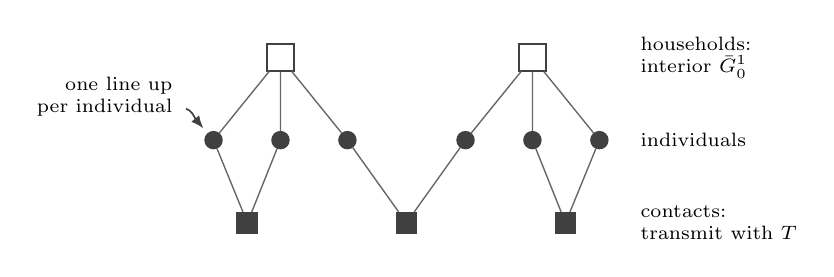
\begin{tikzpicture}
% Three layers, drawn as an inclusion diagram: households (layer 1) above the
% individuals (layer 0) they contain, global contacts (layer 2) below.
\node[cpx,minimum size=3.4mm] (H1) at (0,1.45) {};
\node[cpx,minimum size=3.4mm] (H2) at (3.2,1.45) {};
\node[atm] (a1) at (-0.85,0.40) {}; \node[atm] (a2) at (0,0.40) {};
\node[atm] (a3) at (0.85,0.40) {};
\node[atm] (b1) at (2.35,0.40) {}; \node[atm] (b2) at (3.2,0.40) {};
\node[atm] (b3) at (4.05,0.40) {};
\draw[inc] (H1)--(a1) (H1)--(a2) (H1)--(a3)
           (H2)--(b1) (H2)--(b2) (H2)--(b3);
\node[cpxc,minimum size=2.6mm] (G1) at (1.60,-0.65) {};
\node[cpxc,minimum size=2.6mm] (G2) at (3.62,-0.65) {};
\node[cpxc,minimum size=2.6mm] (G3) at (-0.42,-0.65) {};
\draw[inc] (G1)--(a3) (G1)--(b1) (G2)--(b2) (G2)--(b3) (G3)--(a1) (G3)--(a2);
\node[lb,anchor=west,align=left] at (4.45,1.45) {households:\\ interior $\bar G^{1}_{0}$};
\node[lb,anchor=west,align=left] at (4.45,0.40) {individuals};
\node[lb,anchor=west,align=left] at (4.45,-0.65) {contacts:\\ transmit with $T$};
% the sink: exactly one line leaves each individual upwards
\node[lb,anchor=east,align=right] at (-1.25,0.95) {one line up\\ per individual};
\draw[msg] (-1.20,0.80) to[out=-20,in=150] (-0.98,0.55);
\end{tikzpicture}
\end{adjustbox}
\caption{\textbf{Two levels of mixing is a three-layer chygraph.} Individuals
are atoms; a household is a complex whose interior is the complete graph on its
members; a global contact is a complex holding two individuals. Each individual
lies in exactly one household, Eq.~\eqref{eq:sink}, so an infection arriving in
a household spreads inside it and stops --- the household layer amplifies but
does not conduct. Conduction is the business of the global layer, and the two
enter the threshold in different ways because of it.}
\label{fig:households}
\end{figure}

\begin{calculation}{the final size of a household outbreak}
Let $C_{j}(p)$ be the probability that the random graph $G(j,p)$ is connected,
which satisfies the standard recursion obtained by conditioning on the
component of a fixed vertex,
\[
  C_{j}(p)=1-\sum_{i=1}^{j-1}\binom{j-1}{i-1}C_{i}(p)\,(1-p)^{i(j-i)},
  \qquad C_{1}=1.
\]
The percolation cluster of a given vertex of $K_{n}$ then has size $j$ with
probability
\begin{equation}
  P_{n}(j)=\binom{n-1}{j-1}\,C_{j}(p_{H})\,(1-p_{H})^{\,j(n-j)}:
  \label{eq:Kn}
\end{equation}
choose the other $j-1$ members, require their induced subgraph to be connected,
and require every one of the $j(n-j)$ links to the outside to be absent. For an
epidemic, $j$ is the final size of the household outbreak including the index
case, so
\[
  \bar G^{1}_{0}(y)=\sum_{j}P_{n}(j)\,y^{\,j-1}
\]
counts the \emph{additional} cases, which is what an inclusion into the
household layer transmits. Mixing over households means mixing over the
\emph{size-biased} size distribution $nP(n)/\ave{n}$, because a household is
reached through one of its members and a large household has more of them.

At $n=3$ Eq.~\eqref{eq:Kn} returns
\[
  \begin{aligned}
    \bar G^{1}_{0}(y)&=(3p_{H}^{2}-2p_{H}^{3})y^{2}+2p_{H}(1-p_{H})^{2}y\\
    &\quad+(1-p_{H})^{3}+p_{H}(1-p_{H})^{2},
  \end{aligned}
\]
which is Eq.~\eqref{eq:tripgf} --- the bond-percolated triangle of
Sec.~\ref{sec:structurebystructure}, term for term, with $p_{H}$ where $q$
stood. A three-person household and an over-represented triangle are the same
object with different names, and the mean number of additional cases is
$\mu_{H}=\bar s_{\triangle}(p_{H})=2p_{H}(1+p_{H}-p_{H}^{2})$.
\end{calculation}

What a user of the software has to supply is a dictionary of household sizes.
Everything else --- the size-biasing, the connectivity recursion, the filling of
$\Phi^{0}_{1}(x)=x$ into the table --- follows from the mapping. The
epidemiology enters through one table entry and nothing else.

\section{The household reproduction number}
\label{sec:rstar}
\index{reproduction number|textbf}

Substituting into the threshold tensor of Sec.~\ref{sec:threshold}, with a
Poisson global contact network of mean degree $\ave{k}$ and global
transmissibility $T$, gives
\begin{equation}
  \theta+1=T\bigl[\ave{\bar k}+\mu_{H}\ave{k}\bigr]\equiv R^{\ast},
  \label{eq:Rstar}
\end{equation}
with $\mu_{H}=\bar G^{1\prime}_{0}(1)$ the mean number of \emph{additional}
household members infected.

Equation~\eqref{eq:Rstar} is the household reproduction number of
\citet{ball1997}. It has a plain reading, and the reading is the same
branching argument that has run through the book since
Sec.~\ref{sec:percolation-intro}. A household reached by one global infection
ends up containing $1+\mu_{H}$ cases. The index case makes $T\ave{\bar k}$
further global infections, having used one contact to arrive; each of the
$\mu_{H}$ secondary cases makes $T\ave{k}$, having used none. An outbreak grows
when the total exceeds one.

What has and has not happened here. The epidemiological literature derives $R^{\ast}$ by constructing a branching
process of households and computing its mean offspring number, which is a
purpose-built argument. Here it is a substitution into a tensor that knows
nothing about disease, and the derivation is the same one that produced
Molloy--Reed and the hypergraph threshold in
Sec.~\ref{sec:structurebystructure}. That is the claim about labour that
Chapter~\ref{ch:percolation} opened with, made in a setting where the
purpose-built argument is genuinely well known.

\paragraph{What the branching argument does not give.} $R^{\ast}$ locates the
threshold and stops. The final size of a major outbreak does not follow from
it, and neither does the rate at which that size grows once the threshold is
passed --- the critical amplitude of Sec.~\ref{sec:amplitude}. Both come out of
the same chygraph without further input (Fig.~\ref{fig:householdfig}), and
Table~\ref{tab:households} does both for households of size three on a
Poisson global network with $\ave{k}=2$.
\begin{table}[t]
\centering\small
\begin{tabular}{lccc}
\hline\hline
 & $p_{H}=0$ & $p_{H}=1/2$ & $p_{H}=1$\\
\hline
$\mu_{H}$      & $0$      & $1.25$   & $2$\\
$T_{c}$        & $0.5000$ & $0.2222$ & $0.1667$\\
$B$            & $4.000$  & $5.478$  & $6.667$\\
$S$ at $T=1$   & $0.7968$ & $0.9560$ & $0.9975$\\
\hline\hline
\end{tabular}
\caption{\textbf{Households lower the threshold and steepen the approach to it.} Households of size three on a Poisson global network with $\ave{k}=2$, at three within-household transmission probabilities. $\mu_{H}$ is the mean number of further household infections, $B$ the critical amplitude of Sec.~\ref{sec:amplitude} and $S$ the final size. The $p_{H}=0$ column reduces to bond percolation on a Poisson graph. Generated by \code{figs/epidemics.py}.}
\label{tab:households}
\end{table}
Households do two separable things. They lower the threshold, by a factor of three here. And they steepen the
approach to it: $B$ rises from $4$ to $6.667$, so just above threshold the
outbreak is not merely more likely but larger. The first fact is $R^{\ast}$'s;
the second is not, and it needs one more order of moments.

The $p_{H}=0$ column is the check one wants. With no within-household
transmission the household layer transmits nothing, the chygraph reduces to
bond percolation on a Poisson graph, $T_{c}=1/\ave{k}=1/2$, and $B=4p$ at $p=1$
--- the first row of Table~\ref{tab:amplitudes}, reached down a completely
different code path.

\begin{figure}[t]
\centering
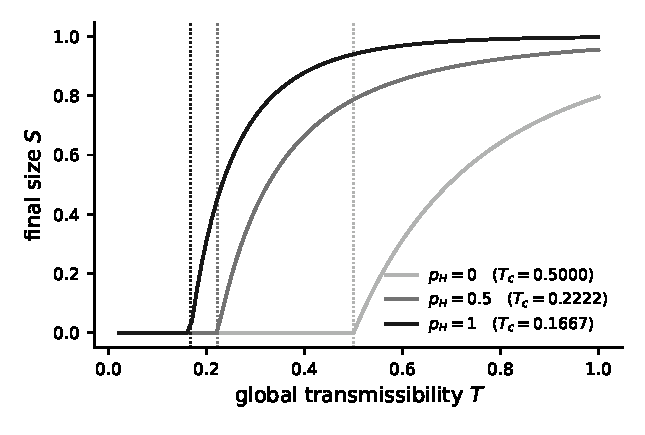
\includegraphics[width=0.9\linewidth]{figs/fig-households.pdf}
\caption{\textbf{Two levels of mixing.} Final size of an SIR epidemic against
the global transmissibility $T$, for households of size three on a Poisson
global contact network with $\ave{k}=2$, at three values of the within-household
transmission probability $p_{H}$. Dotted lines are $R^{\ast}=1$,
Eq.~\eqref{eq:Rstar}. At $p_{H}=0$ the household layer is inert and the curve is
ordinary bond percolation on a Poisson graph. Generated by
\code{figs/epidemics.py}.}
\label{fig:householdfig}
\end{figure}

\paragraph{Loosening the sink.} Equation~\eqref{eq:sink} was the only
epidemiological input, and letting $\Phi^{0}_{1}$ be a genuine degree
distribution instead of the constant $1$ --- individuals belonging to several
groups rather than one --- turns the same chygraph into a \emph{network of
cliques}. That covers SIR with clique-type-dependent transmission, and at
$p_{H}=1$ the connected components of bipartite projections
\citep{fujiki2024proj}. With all cliques of size two it reduces to ordinary bond
percolation and with all of size three to the triangle layer of
Sec.~\ref{sec:structurebystructure} --- two independent code paths that agree.
One dictionary entry separates a household model from a clique network, which
is the sense in which none of this is a family of models.

\section{Contagion inside a group}
\label{sec:groupcontagion}
\index{threshold contagion|textbf}
\index{spinodal}

Everything so far has assumed that one infected member of a group is enough:
the disease enters a household through a single case and spreads by pairwise
contact inside it. Much of what people mean by \emph{higher-order} spreading is
the denial of that assumption. A rumour, a behaviour, a decision to vaccinate
may need reinforcement --- two of three housemates, not one
\citep{watts2002,iacopini2019,stonge2021}. Call it a threshold rule: a group
transmits to a member only when at least $r$ of the others are already
infected.

This looks like a small change and it is not, though the damage is narrower than
it first appears. Chapter~\ref{ch:statmech}'s two steps carry the rule without
modification. What does not carry over is the linear apparatus built on top of
them.

\paragraph{The recursion still closes on one number.} Let $\pi$ be the
probability that a member reached along an inclusion is infected by everything
else attached to it. On a tree the other $c-1$ members of a complex are
independent given $\pi$, so the interior sum of Eq.~\eqref{eq:emitted} is a
binomial tail: a complex of cardinality $c$ fires onto the member entered by
exactly when at least $r$ of the others are infected,
\begin{equation}
  \tau_{c,r}(\pi)=T_{c}\sum_{m\ge r}\binom{c-1}{m}\pi^{m}(1-\pi)^{c-1-m},
  \label{eq:threshtau}
\end{equation}
and the up step is the same product over inclusions as
Eq.~\eqref{eq:Qminus}, with the same bracket: a member reached through layer $m$
escapes only if every one of its other complexes fails to fire, the arriving
inclusion discounted from layer $m$ alone, so
\begin{equation}
  \begin{aligned}
    \pi^{m}&=1-\prod_{l}\bigl[\bar\Phi^{0}_{l}\bigr]_{l=m}
             \bigl(1-\tau_{c_{l},r_{l}}(\pi^{l})\bigr),\\
    \rho&=1-\prod_{l}\Phi^{0}_{l}
          \bigl(1-\tau_{c_{l},r_{l}}(\pi^{l})\bigr),
  \end{aligned}
  \label{eq:threshmap}
\end{equation}
with $\rho$ the infected fraction. This is the two-step recursion of
Sec.~\ref{sec:twosteps} with a threshold interior substituted for a
percolating one, and it carries an arbitrary chy-degree distribution and an
arbitrary mixture of cardinalities and thresholds.

\paragraph{What is lost is the linearisation.} Differentiate
Eq.~\eqref{eq:threshtau} at $\pi=0$. For $r=1$ it gives $T_{c}(c-1)$, the
intra-complex factor of Chapter~\ref{ch:percolation}. For $r\ge2$ it gives
\emph{zero}: $\tau_{c,r}(\pi)\sim\pi^{r}$, so a layer with $r\ge2$ contributes
nothing to the Jacobian of Eq.~\eqref{eq:threshmap} at the trivial fixed point,
whatever its chy-degree. The consequence is visible without any calculation.
With $r\ge2$ a single infected seed cannot activate any group, so it infects
nobody, so $\pi=0$ --- nothing connected to anything --- is not merely a fixed
point but a \emph{stable} one, at every parameter value.
Section~\ref{sec:breakdown} named this exclusion when it arose for
interdependent networks: the transition, if there is one, happens by a
saddle-node bifurcation while the trivial fixed point is still stable, so
$\Lambda=0$ does not locate it, and the threshold tensor of
Sec.~\ref{sec:threshold} --- which is that Jacobian --- reports only the
pairwise layer.

Section~\ref{sec:breakdown}'s proof that group structure alone gives continuous
transitions is untouched by this, and the two are easily confused. That proof
needs the intra-complex function to be a generating function in the
\emph{failure} variable, where all derivatives are non-negative; a threshold
rule is not one, since in $Q=1-\pi$ the failure probability $1-\pi^{r}$ of a
group carries a negative coefficient. So: within the percolation class every
group interaction contributes non-negatively to the curvature $C$ and the onset
is continuous; a threshold rule is outside that class, while remaining inside
the recursion.

\paragraph{The simplest case.} Take a population with two kinds of connection:
Poisson-many pairwise contacts, mean $\ave{k}_{|}$, each transmitting with
probability $T$; and Poisson-many three-member groups, mean
$\ave{k}_{\triangle}$, each transmitting to a member with probability
$T_{\triangle}$ but only when \emph{both} others are infected. Write
\begin{equation}
  \beta_{1}=T\ave{k}_{|},
  \qquad
  \beta_{2}=T_{\triangle}\ave{k}_{\triangle}.
\end{equation}
A Poisson layer is its own excess, $\bar\Phi(x)=\Phi(x)=e^{\ave{k}(x-1)}$, so
$\pi$ and $\rho$ coincide; $\tau_{2,1}=T\rho$ and $\tau_{3,2}=T_{\triangle}\rho^{2}$;
and Eq.~\eqref{eq:threshmap} collapses to
\begin{equation}
  \rho=1-e^{-\beta_{1}\rho-\beta_{2}\rho^{2}}.
  \label{eq:contagion}
\end{equation}
The $\rho^{2}$ is the higher-order physics --- two infected others
required, hence the square --- and everything below is a consequence of it.

\begin{calculation}{where the onset stops being continuous}
Expand the right-hand side of Eq.~\eqref{eq:contagion} about $\rho=0$:
\[
  \rho=\beta_{1}\rho
      +\Bigl(\beta_{2}-\tfrac{\beta_{1}^{2}}{2}\Bigr)\rho^{2}
      +\Bigl(\tfrac{\beta_{1}^{3}}{6}-\beta_{1}\beta_{2}\Bigr)\rho^{3}
      +O(\rho^{4}).
\]
The linear term gives the invasion threshold $\beta_{1}=1$, which involves
$\beta_{2}$ not at all: a seed cannot use the groups, so the groups cannot help
it invade. Setting $\beta_{1}=1$ leaves quadratic coefficient
$\beta_{2}-\tfrac12$ and cubic coefficient $\tfrac16-\beta_{2}$.

When $\beta_{2}<\tfrac12$ the quadratic coefficient is negative, the outbreak
branch leaves the threshold upwards with $\rho\propto(\beta_{1}-1)$, and the
transition is continuous with $\beta=1$ as in Sec.~\ref{sec:amplitude}. When
$\beta_{2}>\tfrac12$ it is positive: the branch leaves \emph{backwards}, exists
below $\beta_{1}=1$, and the transition is discontinuous, with a fold at some
$\beta_{1}<1$. The two are separated by a tricritical point at
\begin{equation}
  \beta_{2}=\tfrac12,
  \label{eq:tricritical}
\end{equation}
where the quadratic term vanishes and the cubic one takes over, giving
$\rho\simeq\sqrt{3(\beta_{1}-1)}$ and the exponent $\beta=\tfrac12$ instead of
$1$. Solving Eq.~\eqref{eq:contagion} numerically at $\beta_{1}-1=10^{-2}$,
$10^{-3}$, $10^{-4}$ gives $\rho/\sqrt{3(\beta_{1}-1)}=0.937$, $0.980$,
$0.994$.

There is no root-finding anywhere in this. Solving Eq.~\eqref{eq:contagion} for
$\beta_{1}$ instead of for $\rho$,
\[
  \beta_{1}(\rho)=\frac{-\ln(1-\rho)-\beta_{2}\rho^{2}}{\rho},
\]
parametrises the whole curve, unstable branch included, and the fold is the
minimum of that function.
\end{calculation}

Figure~\ref{fig:contagion} is the calculation drawn. One dial, $\beta_{2}$,
carries the onset from continuous through tricritical to discontinuous, and at
$\beta_{2}=2$ the fold sits at $\beta_{1}=0.3145$ with $\rho=0.6628$: an
established outbreak survives down to a third of the coupling at which one could
have started. The jump at the invasion threshold is from nothing to
$\rho=0.930$.

\begin{figure}[b]
\centering
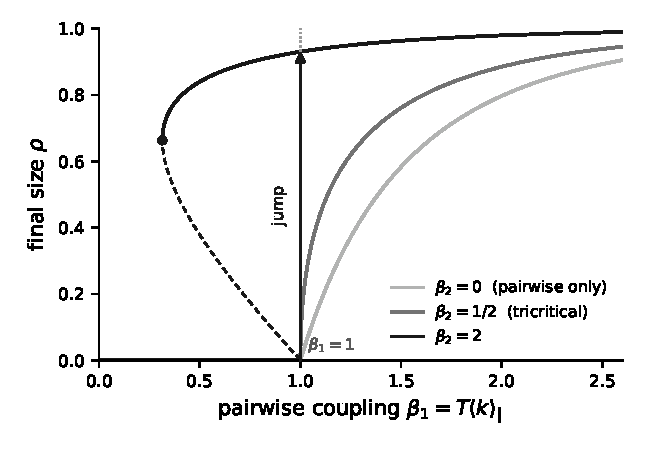
\includegraphics[width=0.9\linewidth]{figs/fig-contagion.pdf}
\caption{\textbf{One dial from continuous to explosive.} Final size against the
pairwise coupling $\beta_{1}$ for Eq.~\eqref{eq:contagion}, at three strengths
$\beta_{2}$ of a group interaction that transmits only when both other members
are infected. Solid lines are stable branches, dashed the unstable one, the
circle the fold. The invasion threshold is $\beta_{1}=1$ whatever $\beta_{2}$;
what $\beta_{2}$ changes is whether the outbreak grows out of it or jumps.
Eq.~\eqref{eq:tricritical} places the boundary at $\beta_{2}=1/2$. Generated by
\code{figs/epidemics.py}.}
\label{fig:contagion}
\end{figure}

Push the dial to the end --- no pairwise route at all, $\beta_{1}=0$ --- and the
invasion threshold disappears rather than moving. No seed can ever start
anything, at any $\beta_{2}$. Yet an outbreak, once present, sustains itself for
all $\beta_{2}>2.4554$, at which point $\rho$ jumps to $0.7153$. A population
with only reinforced transmission cannot be invaded and can be saturated, which
is a statement no threshold calculation would produce, and one a public-health
argument can use.

\paragraph{The equilibrium version of the same thing.} A group that acts only
when all its members agree is Chapter~\ref{ch:ising}'s unanimity interaction:
the simplicial Ising model of \citet{son2026}, whose hyperedges lower the
energy only on their two unanimous configurations. There too the transition is
continuous at small cardinality and discontinuous above a tricritical one, there
too the linear instability of the disordered state is a spinodal rather than the
transition, and there too quoting it as the transition is wrong by ten to fifty
per cent. Chapter~\ref{ch:ising} does that calculation properly, with free
energies. It is the same physics, and the difficulty is the one this section has
already met: a rule that needs several participants at once leaves no linear
instability to locate the transition with.

\section{What higher-order structure does to an outbreak}
\label{sec:epidemics-lessons}

Four things, none of which needs the algebra.

\emph{Groups amplify what reaches them, and it is the amplification that is
counted.} A household does not conduct --- an infection cannot pass through one
household to another, Eq.~\eqref{eq:sink} --- and yet it raises the reproduction
number by a factor of three here, because $\mu_{H}$ multiplies the number of
onward global infections. Conduction and amplification are separate services and
the threshold tensor keeps them in separate entries.

\emph{The amplification saturates.} $\mu_{H}\le n-1$: a household cannot infect
more people than it holds. This is the ``more per branch, fewer branches''
observation of Sec.~\ref{sec:helporhurt} in its most concrete form, and it is
why the fixed-degree and fixed-link-count comparisons of that section come out
with opposite signs.

\emph{Say what is held fixed.} Sec.~\ref{sec:rstar}'s table holds the global
network fixed and adds within-household transmission on top of it, and on that
comparison households help the epidemic a great deal. Hold instead the
\emph{contact budget} fixed --- four contacts per person either way, as
size-three households on a Poisson global network of mean two, against no
households and a Poisson network of mean four, with the same transmissibility
everywhere --- and the sign reverses. The threshold \emph{rises}, from
$T_{c}=0.2500$ to $0.2929$, and at $T=0.3$ the outbreak reaches $5.6\%$ of the
population with households against $31.4\%$ without. Household contacts are
spent repeatedly on the same three people. This is the running thread of
Chapters~\ref{ch:data}, \ref{ch:percolation} and~\ref{ch:giant} appearing once
more, and here it has a public-health reading: whether structure helps or hurts
depends on whether the structured contacts are additional to the rest or taken
out of them.

\emph{Percolation-type spread is always continuous; reinforced spread need not
be.} If one infected contact suffices, the outbreak grows out of its
threshold smoothly, and Sec.~\ref{sec:breakdown} proves this cannot be
otherwise for anything in the percolation class. If several are required, the
outbreak can appear at full size or not at all, cannot be started by a single
seed, and persists below the coupling at which it could have begun. Which r\'egime
a real spreading process is in is an empirical question, and the two make
completely different predictions about what an intervention does.

\section{Checks}
\label{sec:epidemics-checks}

\checkhead{Known results}
Equation~\eqref{eq:Rstar} is verified symbolically against
$T[\ave{\bar k}+\mu_{H}\ave{k}]$ for several household size distributions,
including mixtures of sizes, with $\mu_{H}$ computed independently from the
connectivity recursion; that expression is \citeauthor{ball1997}'s household
reproduction number. Equation~\eqref{eq:Kn} at $n=3$ is checked term by term
against the bond-percolated triangle of Sec.~\ref{sec:structurebystructure},
Eq.~\eqref{eq:tripgf}, symbolically in $p_{H}$. The $p_{H}=0$ column of
Sec.~\ref{sec:rstar}'s table reproduces bond percolation on a Poisson graph,
$T_{c}=1/\ave{k}$ and $B=4$, along a code path that has never heard of
households.

\checkhead{New results}
The critical amplitude for households, and the threshold-rule recursion
Eq.~\eqref{eq:threshmap} with its tricritical point, have no published
counterpart. The amplitudes are obtained by numerical eigenvectors on the full
index set, independently of the symbolic route of Sec.~\ref{sec:amplitude}.
Equation~\eqref{eq:threshmap} is checked against forward simulation of the
contagion on random chygraphs at $n=4\times10^{5}$, over eight combinations of
$\beta_{1}$, $\beta_{2}$ and seed fraction, agreeing to $10^{-3}$ or better in
every case. The tricritical condition Eq.~\eqref{eq:tricritical} is checked in
two ways: symbolically, that the quadratic coefficient at $\beta_{1}=1$ is
$\beta_{2}-\tfrac12$; and numerically, that the fold lies below $\beta_{1}=1$
exactly when $\beta_{2}>\tfrac12$. The exponent $\beta=\tfrac12$ at the
tricritical point is confirmed by solving Eq.~\eqref{eq:contagion} at three
decades of $\beta_{1}-1$.

\checkhead{Partial results}
Everything here is a final size and not a time course, and everything assumes
one infectious period for everyone; Sec.~\ref{sec:sirperc} says what breaks when
it is random. Equation~\eqref{eq:threshmap} inherits Chapter~\ref{ch:overlap}'s
limitation unchanged, since a threshold rule is no more forgiving of overlapping
complexes than a percolating one. And it comes without the apparatus that makes
Chapter~\ref{ch:percolation} quick: with $r\ge2$ the threshold tensor reports
only the pairwise layer, so every transition here is found by following the
branch rather than by linearising, and the edges of a coexistence window are
located one at a time.


% sources
% - manuscript_3, "Epidemics with two levels of mixing"
% - manuscript 2, interacting graphs and hypergraphs
% - the discontinuous-onset material connects forward to Ch. 9's unanimity
%   interaction; keep the two consistent

\part{Statistical mechanics}

\chapter{Potts, and one recursion for both}
\label{ch:potts}

Part~II solved percolation. Part~III solves the Ising model, the hitting set
problem, vertex cover. They have been presented as two subjects that happen to
share a method, and the reader has been asked to take on faith that the second
is worth the first.

They are one subject. This is the chapter that says so, and it is the shortest
in the book because the statement, once set up properly, is short: the
percolation map of Chapter~\ref{ch:percolation} is the $q\to1$ limit of the
cavity recursion for the $q$-state Potts model, complex by complex, and the
Ising model of Chapter~\ref{ch:ising} is the same recursion at $q=2$. Not an
analogy, not a shared structure --- the same equations, at two values of one
parameter. Section~\ref{sec:qlimit} does the limit and
Sec.~\ref{sec:transmission} exhibits the single function that both chapters
have been computing without saying so.

\section{The random-cluster model}
\label{sec:rc}

Fix a graph with edge set $E$. A \emph{configuration} is a subset
$\omega\subseteq E$ of present edges, and the random-cluster model
\citep{fortuin1972} weights it by
\begin{equation}
  W(\omega)=p^{|\omega|}\,(1-p)^{|E|-|\omega|}\,q^{\,k(\omega)},
  \label{eq:rcweight}
\end{equation}
with $k(\omega)$ the number of connected components of $(V,\omega)$ and
$Z_{\mathrm{RC}}=\sum_{\omega}W(\omega)$.

Two parameters, and they do quite different jobs. The first, $p$, is the
familiar one: without the last factor, Eq.~\eqref{eq:rcweight} is exactly
independent bond percolation at occupation probability $p$. The second, $q$, is
a reward for being disconnected. At $q>1$ configurations that fall into many
pieces are favoured, at $q<1$ they are penalised, and at $q=1$ the factor is
$1$ and nothing is favoured at all.

So the first statement of this chapter can be made before any machinery:

\begin{center}
\emph{At $q=1$ the random-cluster measure \textbf{is} bond percolation.}
\end{center}

Exactly, at the value $q=1$; nothing is being taken to a limit. That matters,
because a limit is about to be taken and it is a different one.

Nothing in Eq.~\eqref{eq:rcweight} requires $q$ to be a whole number. It is a
real parameter, $q>0$, and the model is defined along the whole axis. This will
be the point of the chapter: the axis is continuous, the interesting problems
sit at particular values of it, and one calculation covers the axis.

\section{Fortuin--Kasteleyn}
\label{sec:fk}

The reason $q$ has the name it does is that at whole-number values
Eq.~\eqref{eq:rcweight} is a spin model in disguise.

\begin{calculation}{the correspondence}
Give each vertex a state $\sigma_i\in\{1,\dots,q\}$ and couple neighbours that
agree,
\[
  Z_{\mathrm{Potts}}
   =\sum_{\{\sigma\}}\exp\Bigl(\beta J\sum_{\langle ij\rangle}
     \delta_{\sigma_i\sigma_j}\Bigr)
   =\sum_{\{\sigma\}}\prod_{\langle ij\rangle}
     \bigl(1+v\,\delta_{\sigma_i\sigma_j}\bigr),
\]
with $v=e^{\beta J}-1$, using $e^{x\delta}=1+(e^{x}-1)\delta$, which is exact
because $\delta$ is $0$ or $1$. Multiply the product out. Each term selects a subset $\omega$ of edges and
contributes $v^{|\omega|}\prod_{\langle ij\rangle\in\omega}
\delta_{\sigma_i\sigma_j}$; the deltas force every vertex in a component of
$(V,\omega)$ to share one state, so the sum over states gives $q$ choices per
component:
\[
  Z_{\mathrm{Potts}}=\sum_{\omega\subseteq E}v^{|\omega|}\,q^{\,k(\omega)}.
\]
Put $p=v/(1+v)=1-e^{-\beta J}$, so that $v^{|\omega|}=(p/(1-p))^{|\omega|}$, and
multiply by $(1-p)^{|E|}$:
\begin{equation}
  (1-p)^{|E|}\,Z_{\mathrm{Potts}}=Z_{\mathrm{RC}}.
  \label{eq:fk}
\end{equation}
The two models have the same partition function up to a constant, and the
correspondence is a bijection between spin configurations and edge
configurations only after the spins have been summed out. What survives is
Eq.~\eqref{eq:fk} and the dictionary $p=1-e^{-\beta J}$.
\end{calculation}

Equation~\eqref{eq:fk} is the Fortuin--Kasteleyn representation
\citep{fortuin1972}, and it is worth stating what it does and does not say,
because the statement is routinely garbled.

The derivation needs $q$ to be a whole number, because it counted states. So
the identity holds at $q=2,3,4,\dots$ and the models it identifies are the
Ising model at $q=2$ and the Potts models above. Equation~\eqref{eq:rcweight},
on the other hand, needs nothing of the kind and is defined for every $q>0$.
The random-cluster model is therefore the larger object, containing the spin
models at the whole numbers and bond percolation at $q=1$ --- where there is no
spin model at all, since a one-state Potts model has one configuration and no
content. Fortuin and Kasteleyn's own numbering has $\kappa=1$ the percolation
model, $\kappa=2$ the Ising model, $\kappa=3,4,\dots$ the Potts models, and it
is the right way to keep this straight. \emph{Bond percolation is the $q\to1$
limit of the random-cluster model, not of the Potts model.}

\paragraph{Why a limit is mentioned at all.} At $q=1$ every configuration has
weight $p^{|\omega|}(1-p)^{|E|-|\omega|}$ and these sum to one:
$Z_{\mathrm{RC}}(q{=}1)=1$ identically, so $\ln Z$ vanishes and there is no free
energy to differentiate. Percolation's thermodynamics sits one order out, in
the derivative,
\begin{equation}
  \frac{\partial}{\partial q}\ln Z_{\mathrm{RC}}\Big|_{q=1}
    =\bigl\langle k(\omega)\bigr\rangle,
  \label{eq:dlnZ}
\end{equation}
the mean number of clusters --- and the giant component is recovered as the
$q\to1$ limit of the Potts magnetisation with a symmetry-breaking field. Hence
the standard phrase. The measure is \emph{at} $q=1$; the observables are
\emph{limits} at $q=1$. Both halves of that sentence are needed and they are
about different things.

\begin{figure}[t]
\centering
\begin{adjustbox}{max width=\linewidth}
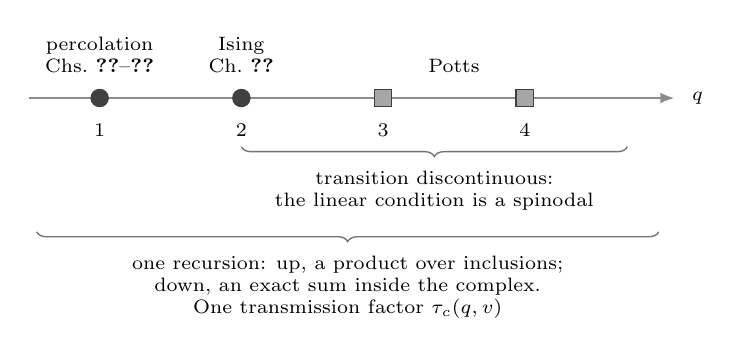
\begin{tikzpicture}
% The q axis. Models sit on it; the two braces underneath say what is shared
% along the whole axis and what changes at q = 2.
\draw[lnk,line width=.8pt,-{Latex[length=1.8mm,width=1.4mm]}] (0,0) -- (8.2,0);
\node[lb,anchor=west] at (8.3,0) {$q$};
\foreach \x/\lab in {0.9/1, 2.7/2, 4.5/3, 6.3/4}{
  \draw[lnk,line width=.7pt] (\x,-0.12) -- (\x,0.12);
  \node[lb,anchor=north] at (\x,-0.20) {\lab};
}
\node[atm] at (0.9,0) {};
\node[atm] at (2.7,0) {};
\node[cpxb,minimum size=2.2mm] at (4.5,0) {};
\node[cpxb,minimum size=2.2mm] at (6.3,0) {};
\node[lb,anchor=south,align=center] at (0.9,0.20)
  {percolation\\ Chs.~\ref{ch:percolation}--\ref{ch:epidemics}};
\node[lb,anchor=south,align=center] at (2.7,0.20)
  {Ising\\ Ch.~\ref{ch:ising}};
\node[lb,anchor=south,align=center] at (5.4,0.20) {Potts};
% what changes at q = 2
\draw[decorate,decoration={brace,amplitude=3.5pt,mirror},draw=black!55,
      line width=.5pt] (2.7,-0.62) -- (7.6,-0.62);
\node[lb,anchor=north,align=center] at (5.15,-0.80)
  {transition discontinuous:\\ the linear condition is a spinodal};
% what is shared along the whole axis
\draw[decorate,decoration={brace,amplitude=3.5pt,mirror},draw=black!55,
      line width=.5pt] (0.1,-1.70) -- (8.0,-1.70);
\node[lb,anchor=north,align=center] at (4.05,-1.88)
  {one recursion: up, a product over inclusions;\\
   down, an exact sum inside the complex.\\
   One transmission factor $\tau_{c}(q,v)$}
;
\end{tikzpicture}
\end{adjustbox}
\caption{\textbf{One axis.} The random-cluster model, Eq.~\eqref{eq:rcweight},
is defined for every $q>0$. Bond percolation sits at $q=1$, the Ising model at
$q=2$, the Potts models above. The whole of Parts~II and~III is one cavity
recursion evaluated along this axis; what changes with $q$ is one function, and
Sec.~\ref{sec:transmission} writes it down. The upper brace marks the other
thing that changes: above $q=2$ the ferromagnetic transition on a random graph
is discontinuous, and the linear instability stops being the transition.}
\label{fig:qaxis}
\end{figure}

\section{The limit, on a chygraph}
\label{sec:qlimit}

Now the claim. Chapter~\ref{ch:percolation} wrote down
Eqs.~\eqref{eq:Qminus}--\eqref{eq:Qplus} from a connectivity argument, with no
Hamiltonian anywhere. Chapter~\ref{ch:statmech} will write down a cavity
recursion for a general model on the same chygraph. The claim is that the first
is the $q\to1$ limit of the second, complex by complex, with the intra-complex
generating function $\bar G$ of Sec.~\ref{sec:ensembles} appearing exactly where
the interior sum was.

\begin{calculation}{the limit, done on a link}
Give member $j$ of a complex an unnormalised message: weight $1$ on one
distinguished state and weight $y_{j}$ on each of the other $q-1$ states. The
complex emits onto member $i$ the pair of sums $Z_{a\to i}(\sigma_{i})$ with
$\sigma_{i}$ distinguished or not, and only their ratio
\[
  \rho_{a\to i}=\frac{Z_{a\to i}(\sigma_{i}\ \text{not distinguished})}
                     {Z_{a\to i}(\sigma_{i}\ \text{distinguished})}
\]
matters. At a member belonging to several complexes the messages multiply,
$y_{i\to b}=\prod_{a\ne b}\rho_{a\to i}$, which is already the shape of
Eq.~\eqref{eq:Qminus}.

Take the complex to be a single link $\{i,j\}$, carrying $1+v\delta$. If
$\sigma_{i}$ is distinguished, $j$ either matches it --- weight $1$, bond
$1+v$ --- or takes one of the $q-1$ other states, weight $y_{j}$ each:
\[
  Z(\text{dist.})=(1+v)+(q-1)y_{j}.
\]
If $\sigma_{i}$ is one fixed non-distinguished state, $j$ may match it
($y_{j}$, bond $1+v$), take the distinguished state ($1$), or take one of the
remaining $q-2$ states ($y_{j}$ each):
\[
  Z(\text{not dist.})=(1+v)y_{j}+1+(q-2)y_{j}.
\]
Both are polynomials in $q$, so both continue to real $q$ on their own. At
$q=1$,
\[
  \rho=\frac{1+v\,y_{j}}{1+v}=(1-p)+p\,y_{j},
  \qquad p=\frac{v}{1+v},
\]
which is $\bar G^{1}_{0}$ for a link --- exactly the entry
Chapter~\ref{ch:percolation} used, arrived at from the Potts model instead of
from a connectivity argument.
\end{calculation}

The general case is the same computation with the state sum organised by which
members share a state. Partition the members of the complex into blocks of
equal state; the interaction depends only on that partition, and the number of
ways to give the blocks distinct states is a falling factorial
$q(q-1)\cdots$, a polynomial in $q$. So the interior sum is a polynomial in $q$
however large the complex, and continuing it to $q=1$ needs no interpretation.
Doing so gives
\begin{equation}
  \lim_{q\to1}\rho_{a\to i}(y)=\bar G_{a}(y),
  \label{eq:qonelimit}
\end{equation}
with $\bar G_{a}$ the generating function of which members of $a$ are reachable
from $i$ under bond percolation inside $a$ --- the object of
Sec.~\ref{sec:definition}, definition for definition. Substituted into
$y_{i\to b}=\prod_{a\ne b}\rho_{a\to i}$, Eq.~\eqref{eq:qonelimit} \emph{is}
Eqs.~\eqref{eq:Qminus}--\eqref{eq:Qplus}.

This has been checked symbolically in the bond probability, with distinct
$y_{j}$ on every member, for complexes that are cliques up to $K_{5}$ and for
paths, against the reachability generating function computed by direct
enumeration. For a triangle it returns Eq.~\eqref{eq:tripgf}, the enumeration
of Sec.~\ref{sec:structurebystructure}, term by term.

\paragraph{What this explains.} Chapter~\ref{ch:percolation} said that a
percolation message is a single number and left it as a fact about percolation.
It is not: it is a fact about the ferromagnetic problem at every $q$. The
message here is one number for all $q$, because the interaction singles out
``agreeing'' and leaves the $q-1$ ways of disagreeing symmetric. What the
percolation limit does is not reduce the message but simplify its
\emph{composition}: at $q=1$ the number is a probability and complexes combine
by multiplying probabilities of failure, which is arithmetic a reader has
already. That is the whole of why Part~II could come first.

\section{The transmission factor}
\label{sec:transmission}

Both parts of the book have, in fact, been computing one function.

The recursion always has the symmetric fixed point $y\equiv1$: every state
equally likely, which at $q=1$ reads as nothing being connected to anything.
Linearising about it, each traversal of a complex contributes
\begin{equation}
  \tau_{c}(q,v)=\frac{\partial\rho_{a\to i}}{\partial y_{j}}\bigg|_{y=1},
  \label{eq:taudef}
\end{equation}
the \emph{transmission} of a cardinality-$c$ complex to one of its members. For
a link the whole of it is
\begin{equation}
  \tau_{2}(q,v)=\frac{v}{q+v},
  \qquad v=e^{\beta J}-1,
  \label{eq:tau2}
\end{equation}
and this one expression is the hinge of the book. At $q=1$ it is
$v/(1+v)=p$: the bond occupation probability, and
Chapter~\ref{ch:percolation}'s entire link layer. At $q=2$ it is
$v/(2+v)=\tanh(\beta J/2)$, which is $\tanh(\beta J_{\mathrm{I}})$ once one
notices that $\delta_{\sigma\sigma'}=(1+\sigma\sigma')/2$ makes a Potts bond of
coupling $J$ an Ising bond of coupling $J/2$ --- the textbook Ising cavity
factor, and Chapter~\ref{ch:ising}'s entire link layer.

The interior earns its keep at $c=3$. There
\begin{equation}
  \tau_{3}(q,v)=\frac{v\,(q+3v+v^{2})}{q^{2}+3qv+3v^{2}+v^{3}},
  \label{eq:tau3}
\end{equation}
and the two values give
\begin{equation}
  \tau_{3}\big|_{q\to1}=p\,(1+p-p^{2}),
  \qquad
  \tau_{3}\big|_{q=2}=\frac{t}{1-t+t^{2}},
  \quad t=\tanh\beta J_{\mathrm{I}}.
  \label{eq:tau3limits}
\end{equation}
The first is half of $\bar s_{\triangle}(p)=2p(1+p-p^{2})$, the bond-percolated
triangle of Sec.~\ref{sec:structurebystructure} --- half, because $\tau$ is
per member and a triangle has two others. The second is the triangle
transmission that Chapter~\ref{ch:ising} builds its headline result on. Two
formulas that look unrelated, derived in different chapters from different
arguments, are Eq.~\eqref{eq:tau3} at $q=1$ and $q=2$
(Fig.~\ref{fig:transmission}).

\begin{figure}[t]
\centering
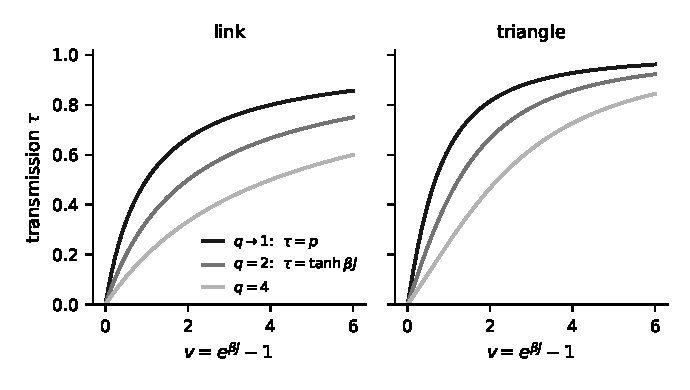
\includegraphics[width=\linewidth]{figs/fig-potts.pdf}
\caption{\textbf{One transmission factor, with $q$ as a dial.}
Equations~\eqref{eq:tau2} and~\eqref{eq:tau3} against the coupling. At $q\to1$
the curve is the percolation quantity of Chapter~\ref{ch:percolation} --- the
bond probability for a link, $\bar s_{\triangle}/2$ for a triangle --- and at
$q=2$ it is the Ising cavity factor of Chapter~\ref{ch:ising}. Nothing changes
between the two but the number in the denominator. Generated by
\code{figs/potts.py}.}
\label{fig:transmission}
\end{figure}

\paragraph{One condition, two famous thresholds.} What is done with $\tau$ is
Chapter~\ref{ch:statmech}'s business in general --- it becomes the branching
matrix, and the transition is at $\det(I-B)=0$. For the simplest case, a single
layer of $c$-cliques with excess chy-degree $\ave{\bar k}$, the condition reads
\begin{equation}
  (c-1)\,\tau_{c}(q,v)\,\ave{\bar k}=1,
  \label{eq:branchcond}
\end{equation}
$c-1$ being the members reached inside the complex and $\ave{\bar k}$ the
complexes reached from each. For a graph, $c=2$, Eq.~\eqref{eq:tau2} makes this
linear in $q$:
\begin{equation}
  v_{c}=\frac{q}{\ave{\bar k}-1}.
\end{equation}
At $q=1$ that is $p_{c}=v_{c}/(1+v_{c})=1/\ave{\bar k}$, which is
Eq.~\eqref{eq:molloyreed}, Molloy and Reed. At $q=2$ it is
$\tanh\beta J_{\mathrm{I}}=1/\ave{\bar k}$, the Bethe-lattice Ising critical
temperature. The two most quoted results in the two halves of this book are one
line evaluated at two points.

\paragraph{Where the analogy stops, and it stops sharply.} Above $q=2$ the
ferromagnetic transition on a random graph is \emph{discontinuous}, and
Eq.~\eqref{eq:branchcond} then locates the loss of stability of the disordered
state rather than the transition. The ordered branch exists below it. Iterating
the graph recursion at excess degree $2$ from an ordered start, the branch first
survives at
\begin{center}\small
\begin{tabular}{lcccc}
\hline\hline
$q$ & $2$ & $3$ & $4$ & $6$\\
\hline
Eq.~\eqref{eq:branchcond} & $2.000$ & $3.000$ & $4.000$ & $6.000$\\
ordered branch from & $2.000$ & $2.828$ & $3.464$ & $4.472$\\
$v_{c}$ too high by & --- & $5.7\%$ & $13.4\%$ & $25.5\%$\\
\hline\hline
\end{tabular}
\end{center}
At $q=2$ the two coincide and the transition is continuous, which is why
Chapter~\ref{ch:ising} may use the linear condition and why
Chapter~\ref{ch:percolation} may at $q=1$. Above it they do not, and the true
transition needs a free-energy comparison inside the coexistence window. This
is the third time the book has met that distinction --- Sec.~\ref{sec:breakdown}
for interdependent networks, Sec.~\ref{sec:groupcontagion} for threshold
contagion --- and it will be met a fourth time in
Chapter~\ref{ch:ising}'s unanimity interaction. A linear instability is a
linear instability. Whether it is also a transition is a separate question and
has to be asked separately.

\section{Site occupation is not a limit}
\label{sec:site}

One confusion is worth heading off, because the formalism does both things and
they look alike.

Bond occupation is the random-cluster parameter $p$, the first factor of
Eq.~\eqref{eq:rcweight}, and it is a coupling: at $q=1$ it \emph{is} the
percolation probability, at $q=2$ it is a temperature through
$p=1-e^{-\beta J}$. Site occupation is nothing of the sort. It is a statement
about which vertices are there at all, and it enters as
Sec.~\ref{sec:map} said it does --- by thinning the generating functions,
$\Phi\to1-p+p\Phi$, which is a change to the ensemble the model lives on and
not to the model.

So the two occupation probabilities that run through Part~II are not two
limits of one thing. Site--bond percolation is the $q=1$ random-cluster model
on a diluted ensemble; the diluted Ising model is the $q=2$ random-cluster
model on the same ensemble. Dilution and $q$ are orthogonal, and the mapping
table of Chapter~\ref{ch:percolation} handles the first while this chapter
handles the second.

\section{Why the book is arranged the way it is}
\label{sec:arrangement}

Percolation came first, and by Sec.~\ref{sec:transmission} the reason is
visible and is not that percolation is more important.

At $q=1$ the interior sum, which for a general model is a sum over $q^{c}$
configurations weighted by a Hamiltonian, collapses into a count of which
members are reachable from which. That count is a generating function, the
composition rule is multiplication of probabilities, and the whole apparatus can
be stated to somebody who has met a branching process and nothing else. Every
structural idea in the book --- layers, chy-degrees, the excess bracket, the
threshold tensor, what a complex's interior contributes --- is present at $q=1$
and can be learned there for the price of arithmetic.

What Part~III adds is not a new recursion. It is a heavier message. The
$q$-state ferromagnet keeps a single number all the way along
Fig.~\ref{fig:qaxis}'s axis, which is why this chapter is short.
Chapter~\ref{ch:hittingset} does not: its fields collapse onto integers in the
hard limit and become a whole distribution over fields once replica symmetry
breaks. Chapter~\ref{ch:cover} needs three states rather than one, because a
node on a cavity branch ends leaf-ready, deleted or core-side, and a scalar
cannot say which.
Chapter~\ref{ch:colouring} is this chapter's own model at the opposite sign
--- proper colouring is the antiferromagnetic $q$-state Potts model at zero
temperature --- and Chapter~\ref{ch:satisfiability} is the same construction
with one assignment forbidden per clause.

The organising fact of the book is the one Fig.~\ref{fig:qaxis} draws. There is
one recursion. It goes up through a chy-degree and down through the interior of
a complex, the interior is summed exactly and the rest of the chygraph never
sees how, and what distinguishes one problem from another is what the message
carries. Everything from here to Chapter~\ref{ch:overlap} is that sentence with
a different message substituted, and Chapter~\ref{ch:overlap} is what happens
when the sentence stops being true.

\section{Checks}
\label{sec:potts-checks}

Equation~\eqref{eq:qonelimit} is verified symbolically in the bond probability,
with an independent $y_{j}$ on each member so that no symmetry is being relied
on, for complexes that are $K_{2}$, $K_{3}$, $K_{4}$, $K_{5}$ and paths on
three and four vertices, against the reachability generating function obtained
by enumerating all $2^{|E|}$ bond configurations of the interior. In the
symmetric case it is checked against the independent implementation of
$\bar G$ used in Chapters~\ref{ch:percolation}--\ref{ch:epidemics}.

The other end of the axis is checked the same way: at $q=2$, with
$y_{j}=e^{-2h_{j}}$, the emitted ratio is $e^{-2u}$ with $u$ the Ising cavity
field, verified against an independent enumeration of the Ising interior for
$K_{2}$, $K_{3}$ and $K_{4}$. So the interior sum of this chapter reproduces
Chapter~\ref{ch:percolation}'s at one end and Chapter~\ref{ch:ising}'s at the
other, and neither of those two was written with the other in mind.

Equations~\eqref{eq:tau2} and~\eqref{eq:tau3} are obtained by differentiating
that interior sum, and their limits Eq.~\eqref{eq:tau3limits} are checked
against the closed forms the two chapters quote. The linear threshold
$v_{c}=q/(\ave{\bar k}-1)$ is solved symbolically and confirmed to return
$p_{c}=1/\ave{\bar k}$ at $q=1$ and $\tanh\beta J=1/\ave{\bar k}$ at $q=2$. The
table in Sec.~\ref{sec:transmission} comes from iterating the recursion, and its
$q=2$ column agreeing with Eq.~\eqref{eq:branchcond} to four digits is what
says the iteration is right where the answer is independently known.


% sources
% - the retired manuscript's Sec. I, the Fortuin-Kasteleyn paragraph (git
%   history, commit 5ebd892). Keep the statement
%   exact: bond percolation is the q -> 1 limit of the RANDOM-CLUSTER model,
%   FK's kappa = 1; kappa = 2 Ising; kappa = 3, 4, ... Potts. Site occupation
%   enters by thinning the generating functions, not as a separate limit.

\chapter{Statistical mechanics on chygraphs}
\label{ch:statmech}

There is a point in the study of disordered systems at which the model stops
mattering. A magnet, a minimum vertex cover and a random Boolean formula have
nothing in common as subject matter --- one is physics, one is combinatorial
optimisation, one is logic --- and the same recursion solves all three. It has
been rediscovered often enough to have collected a name in each field: the
Bethe--Peierls approximation, the cavity method, belief propagation. What
distinguishes the three problems is not the recursion. It is only what one
message is required to carry: a number, a distribution, a warning.

This chapter takes that observation seriously enough to write it down once.

Chapter~\ref{ch:potts} claimed that percolation and the Ising model are one
recursion at two values of a parameter, and checked it at both values. That is a
claim about two special cases. This chapter writes the recursion down for
an arbitrary interaction inside a complex, so that the claim stops being about
special cases and becomes the method. Nothing in the chapter has appeared
elsewhere.

The generalisation is one substitution, and Sec.~\ref{sec:substitution} states
it before anything else, because everything afterwards is bookkeeping around
it. The bookkeeping is done once here: the same two steps,
the same branching matrix and the same free energy serve
Chapters~\ref{ch:ising}--\ref{ch:satisfiability} without being rederived.

\section{One substitution}
\label{sec:substitution}

Percolation's message was a number: $Q^{ml}_{i}$, the probability that an
inclusion leads nowhere. The map, Eqs.~\eqref{eq:Qminus}--\eqref{eq:Qplus},
combined those numbers by evaluating generating functions at them and
multiplying.

For a general model the message is a \emph{cavity field} --- how strongly one
part of the chygraph tells another to point up rather than down --- and, at the
level of an ensemble rather than one realisation, a whole distribution of
cavity fields. So make one substitution:

\begin{center}
\emph{the argument of a generating function becomes a measure,\\
and the product becomes a convolution.}
\end{center}

Concretely, let a generating function act on a measure by
\begin{equation}
  \Phi^{l}_{k}\ast Q=\sum_{n}p^{lk}_{n}\,Q^{\ast n},
  \qquad
  \Phi^{l}_{k}(x)=\sum_{n}p^{lk}_{n}x^{n},
  \label{eq:conv}
\end{equation}
the $n$-fold convolution weighted by the chy-degree distribution. Writing
$Q^{lk}$ for the law of the field a layer-$k$ complex emits onto a layer-$l$
complex, the law $P^{ml}$ of the field a layer-$l$ complex sends up into a
layer-$m$ complex is
\begin{equation}
  P^{ml}=\delta_{B}\ast\Bigl(\ast_{k}\,
    \bigl[\bar\Phi^{l}_{k}\bigr]_{k=m}\!\ast\,Q^{lk}\Bigr),
  \label{eq:ensemblemap}
\end{equation}
with $\delta_{B}$ the point mass at the external field $B$ --- the letter
Eq.~\eqref{eq:Hising} uses, and the branching matrix below is the only other
$B$ in the chapter, always either carrying two layer indices or standing inside
$\det(I-B)$ --- and
$[\bar\Phi]_{k=m}$ the same bracket as Fig.~\ref{fig:themap} --- excess on the
layer arrived through, ordinary on every other. Nothing else about
Chapter~\ref{ch:percolation}'s index structure has changed. The layers, the
directions of arrival, the discounting of the inclusion one came in by: all of
it survives verbatim, because none of it was about what the message contained.

Two sanity checks come for free, and they say what the substitution costs.

Put $Q^{lk}=\delta_{u}$, a point mass at a single number. Every convolution
collapses to a product and Eq.~\eqref{eq:ensemblemap} \emph{is} the percolation
map. Percolation is the case in which no distribution is needed, which
Chapter~\ref{ch:potts} explained: at $q=1$ the number is a probability and the
composition is multiplication.

And the first moment of a convolution is the sum of the first moments of its
factors. So linearising Eq.~\eqref{eq:ensemblemap} about the trivial fixed
point gives a linear operator with the same index structure as
Sec.~\ref{sec:threshold}'s tensor --- which is Sec.~\ref{sec:branching}, and it
is why the threshold calculation of Part~II is reusable rather than merely
analogous.

\section{The two steps}
\label{sec:twosteps}

A message lives on a directed inclusion and is updated from every incoming
message except the one it came from. On a chygraph that update has two halves,
and they are of quite different character (Fig.~\ref{fig:twosteps}).

\subsection{Up: a convolution}
\label{sec:upstep}
\index{convolution}

On one realisation, what a node tells a complex it belongs to is the sum of
what its \emph{other} complexes have told it:
\begin{equation}
  h_{i\to a}=B+\sum_{b\ni i,\ b\ne a}u_{b\to i}.
  \label{eq:up}
\end{equation}
Fields add. That is the up step, and it is why the ensemble
version, Eq.~\eqref{eq:ensemblemap}, is a convolution: the law of a sum of
independent terms is the convolution of their laws, and the generating function
supplies how many terms there are.

Equation~\eqref{eq:up} is also where the treelike assumption sits, ahead of
Sec.~\ref{sec:assumes}. Adding the $u_{b\to
i}$ independently is exact only if the complexes at $i$ carry independent
information --- if they meet only at $i$. Section~\ref{sec:treelike} said what
that costs and Chapter~\ref{ch:overlap} pays it.

\subsection{Down: an exact sum inside the complex}
\label{sec:downstep}
\index{interior sum|textbf}

The other half is where percolation and statistical mechanics part company. For
a complex holding $c$ members with internal energy $-\beta H(\sigma)$, the field
it emits onto member $0$ given the cavity fields of the others is
\begin{equation}
  \begin{split}
    u&=\tfrac12\ln\frac{\bar{Z}(\sigma_{0}=+1)}{\bar{Z}(\sigma_{0}=-1)},\\
    \bar{Z}(\sigma_{0})&=\!\!\sum_{\sigma_{1}\dots\sigma_{c-1}}\!\!
      e^{-\beta H(\sigma)+\sum_{j}h_{j}\sigma_{j}}.
  \end{split}
  \label{eq:emitted}
\end{equation}
That sum is done \emph{exactly}, at a cost exponential in $c$ and independent of
everything outside the complex.

Equation~\eqref{eq:emitted} reads like a definition and is not. What the complex
has to tell member $0$ is the whole of its effect on that member, which is the
function $\hat\nu(\sigma_{0})\propto \bar{Z}(\sigma_{0})$. A function of one Ising
variable takes two values, and only their ratio is used, because the message
enters a normalised measure. So the message is one number however large the
complex is --- the enumeration behind it grows as $2^{c}$, what comes out of it
does not --- and writing that number in the exponential form the up step needs,
$\hat\nu(\sigma_{0})\propto e^{u\sigma_{0}}$, fixes $e^{u}/e^{-u}=\bar{Z}(+1)/\bar{Z}(-1)$,
which is Eq.~\eqref{eq:emitted}. The $\tfrac12$ is there because
$\sigma_{0}=\pm1$ rather than $0,1$. It is the same parameterisation that makes
Eq.~\eqref{eq:up} a sum: messages compose by multiplication, and $h$ is the
exponent in which multiplication is addition.

At $c=2$ this returns what Chapter~\ref{ch:introduction} already had. One other
member and one bond give
\begin{align*}
  \bar{Z}(\sigma_{0})&=\sum_{\sigma_{1}}
    e^{\beta J\sigma_{0}\sigma_{1}+h_{1}\sigma_{1}}
    =2\cosh(\beta J\sigma_{0}+h_{1}),\\
  u&=\tfrac12\ln\frac{\cosh(\beta J+h_{1})}{\cosh(\beta J-h_{1})}
   =\mathrm{atanh}\bigl[\tanh\beta J\,\tanh h_{1}\bigr],
\end{align*}
which is the link message of Sec.~\ref{sec:cavity}, and near $h_{1}=0$ it is
$u\simeq t\,h_{1}$ with $t=\tanh\beta J$. That comparison also fixes the units,
which change here and are worth stating once: in Chapter~\ref{ch:introduction} a
field is an energy and $\beta$ is written out, while from
Eq.~\eqref{eq:emitted} onwards it is absorbed, the $h$ here being the $\beta h$
there. Absorbing it is what lets $u'$ below be a pure number. The interior sum
itself, for any $-\beta H$, is \code{cavity.\allowbreak emitted\_\allowbreak field}.

Three properties of Eq.~\eqref{eq:emitted} carry the chapter.

\emph{The Hamiltonian appears here and nowhere else.} Everything upstream and
downstream is structure. Changing the model means passing a different
$-\beta H$ to one routine, which is why Chapters~\ref{ch:ising}
to~\ref{ch:cover} are substitutions rather than derivations, and why the
unanimity interaction of Sec.~\ref{sec:unanimity} needed nothing new.

\emph{Percolation could compress this and a general model cannot.} Reachability
factorises --- whether $i$ reaches $j$ inside the complex does not depend on
what happens outside it --- so Chapter~\ref{ch:percolation} could reduce the
whole interior to one component-size generating function $\bar G$. An
interaction does not factorise and has to be summed. Chapter~\ref{ch:potts}
made this precise from the other side: Eq.~\eqref{eq:qonelimit} is exactly the
statement that the sum \emph{becomes} $\bar G$ as $q\to1$.

\emph{This is what promoting a motif to a complex buys.} A triangle treated as
three links is a loop and breaks the tree assumption. A triangle treated as one
complex has its loop \emph{inside} Eq.~\eqref{eq:emitted}, where it is summed
over exactly and nothing outside ever learns it was there. The price is $2^{c}$,
and for the motifs one actually finds in data --- Chapter~\ref{ch:data}'s
cliques run to a handful of members --- that price is nothing.

\begin{figure}[t]
\centering
\begin{adjustbox}{max width=0.98\linewidth}
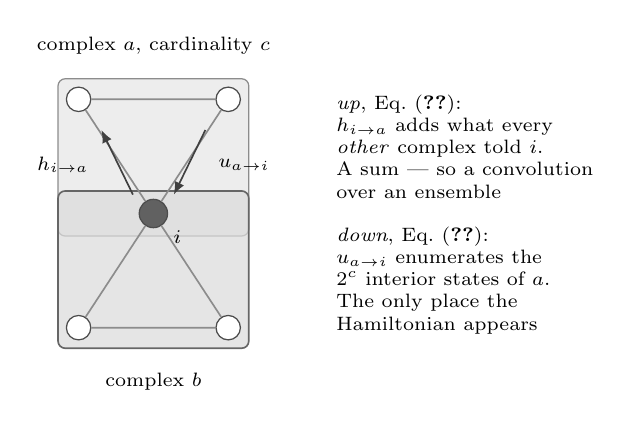
\begin{tikzpicture}
% Node i sits in two complexes, which meet only at i. Up is a sum over the
% others; down is an enumeration inside one of them. The two complexes carry
% different greys so that the shared node reads as a meeting point rather than
% as the overlap of Ch. 13, which is drawn in one grey on purpose.
\node[hub] (i) at (0,0) {};
\node[lb,anchor=north west] at (0.13,-0.10) {$i$};
% complex a, above: its interior is drawn, because the interior is the point
\node[nd] (a1) at (-0.95,1.45) {};
\node[nd] (a2) at (0.95,1.45) {};
\draw[lnk] (i)--(a1) (i)--(a2) (a1)--(a2);
\begin{scope}[on background layer]
  \node[cx,fit=(i)(a1)(a2)] (A) {};
\end{scope}
\node[lb,anchor=south] at (0,1.90) {complex $a$, cardinality $c$};
% complex b, below
\node[nd] (b1) at (-0.95,-1.45) {};
\node[nd] (b2) at (0.95,-1.45) {};
\draw[lnk] (i)--(b1) (i)--(b2) (b1)--(b2);
\begin{scope}[on background layer]
  \node[cxb,fill opacity=0.72,fit=(i)(b1)(b2)] (B) {};
\end{scope}
\node[lb,anchor=north] at (0,-1.90) {complex $b$};
% the two messages, on the a side
\draw[msg] (-0.26,0.24) -- (-0.66,1.06);
\node[lb,anchor=east] at (-0.70,0.62) {$h_{i\to a}$};
\draw[msg] (0.66,1.06) -- (0.26,0.24);
\node[lb,anchor=west] at (0.70,0.62) {$u_{a\to i}$};
% what each step is
\node[lb,anchor=west,align=left] at (2.20,0.85)
  {\emph{up}, Eq.~\eqref{eq:up}:\\
   $h_{i\to a}$ adds what every\\
   \emph{other} complex told $i$.\\
   A sum --- so a convolution\\
   over an ensemble};
\node[lb,anchor=west,align=left] at (2.20,-0.85)
  {\emph{down}, Eq.~\eqref{eq:emitted}:\\
   $u_{a\to i}$ enumerates the\\
   $2^{c}$ interior states of $a$.\\
   The only place the\\
   Hamiltonian appears};
\end{tikzpicture}
\end{adjustbox}
\caption{\textbf{The two steps.} A node passes up the sum of what its other
complexes have told it, Eq.~\eqref{eq:up}; a complex passes down the field
implied by an exact enumeration of its own interior, Eq.~\eqref{eq:emitted}.
The asymmetry is the content. The up step knows nothing of the model and the
down step knows nothing of the rest of the chygraph, so a new model changes one
routine and a new structure changes the other, and neither disturbs the other.
Compare Fig.~\ref{fig:themap}, which is this picture with a number in place of
each message.}
\label{fig:twosteps}
\end{figure}

\section{The branching matrix}
\label{sec:branching}
\index{branching matrix|textbf}

The transition follows from linearising both steps about the trivial fixed
point, where every field vanishes. The down step, Eq.~\eqref{eq:emitted},
responds to each of the complex's other members separately and, at that point,
with the same derivative for each, the interior being symmetric under permuting
them:
\begin{equation}
  \delta u_{a\to i}=u'\!\!\sum_{j\in a\setminus i}\!\delta h_{j\to a},
  \qquad
  u'=\frac{\partial u}{\partial h}\bigg|_{\text{trivial}}.
  \label{eq:uprime}
\end{equation}
The up step, Eq.~\eqref{eq:up}, then adds what the node's other complexes have
sent, $\delta h_{i\to a}=\sum_{b\ni i,\,b\ne a}\delta u_{b\to i}$. Composing
the two, a perturbation is multiplied by $u'$ once per complex traversed and
fanned out twice: over the $c-1$ other members of that complex, and over the
other complexes at the node it lands on. Only the first of the three factors
knows the model. So every traversal of a complex carries one number, $u'$, and
nothing else of the interaction survives the linearisation; the two counting
factors are structure, and assembling them is all
Eqs.~\eqref{eq:branch}--\eqref{eq:sbaru} below do.

That number has been met already. It is Chapter~\ref{ch:potts}'s transmission
$\tau_{c}$, Eq.~\eqref{eq:taudef}, for the case where the interior is a Potts
interaction --- the same derivative of the same emitted quantity at the same
fixed point. For the Ising interaction of Chapter~\ref{ch:ising} it is
$\tau_{c}(2,v)$, verified for $c=2,3,4$: $u'=t$, $t/(1-t+t^{2})$ and
$(t+t^{3})/(1-2t+3t^{2})$ with $t=\tanh\beta J$.

\paragraph{Reusing the threshold tensor.} Because $u'$ enters as a single factor
per traversal, the whole apparatus of Sec.~\ref{sec:threshold} applies to any
model with one substitution,
\begin{equation}
  \ave{s}\ \longrightarrow\ \ave{s\,u'},
  \qquad
  \ave{\sbar}\ \longrightarrow\ \ave{\sbar\,u'},
  \label{eq:reweight}
\end{equation}
an elementwise reweighting that leaves the index structure, the block layout
and the determinant untouched. The weight belongs on the intra-complex channel,
because the interaction lives inside a complex; the chy-degree step is a relay
and carries weight one, so $\ave{\kappa}$ and $\ave{\kbar}$ are left alone.
Replacing $u'$ by $u'^{2}$ throughout gives
the de Almeida--Thouless line instead of the ferromagnetic one, which is
Chapter~\ref{ch:ising}'s spin-glass boundary for the price of a square.

\paragraph{The matrix.} Collecting the two steps: arriving at a node through a
layer-$l$ complex, it belongs to $\ave{\kbar}_{m}$ further layer-$m$ complexes
when $m=l$ and $\ave{\kappa}_{m}$ otherwise --- Chapter~\ref{ch:percolation}'s
bracket again --- and each such complex offers some number of other members,
each carrying $u'$. So the branching matrix on the $L$ complex layers is
\begin{equation}
  B_{lm}=\Bigl[\ave{\kbar}_{m}\delta_{lm}
              +\ave{\kappa}_{m}(1-\delta_{lm})\Bigr]
         \bigl\langle \sbar\,u'\bigr\rangle_{m},
  \label{eq:branch}
\end{equation}
\begin{equation}
  \bigl\langle \sbar\,u'\bigr\rangle_{m}
    =\sum_{c}\frac{c\,p^{(m)}_{c}}{\ave{c}_{m}}\,(c-1)\,u'(c),
  \label{eq:sbaru}
\end{equation}
and the transition is at
\begin{equation}
  \det\bigl(I-B\bigr)=0.
  \label{eq:det}
\end{equation}

The linear algebra is $L\times L$ however large the complexes are. Cardinality
enters only through Eq.~\eqref{eq:sbaru}, and the number of layers is two or
three for everything in this book. Doing the interior sum locally is what buys
that: it is expensive, and its expense never propagates.

When a layer carries a single cardinality $c_{m}$ --- which is how every layer
in Chapters~\ref{ch:ising}--\ref{ch:cover} is built ---
Eq.~\eqref{eq:sbaru} collapses and
\begin{equation}
  B_{lm}=\Bigl[\ave{\kbar}_{m}\delta_{lm}
              +\ave{\kappa}_{m}(1-\delta_{lm})\Bigr](c_{m}-1)\,u'_{m}.
  \label{eq:branchsingle}
\end{equation}
For one layer this is $(c-1)\,u'\ave{\kbar}=1$, which is
Eq.~\eqref{eq:branchcond} --- the condition Chapter~\ref{ch:potts} wrote down
and deferred to here.

A complex is not sampled uniformly when it is reached by following one of its
inclusions. A complex of cardinality $c$ has $c$ inclusions, so it is reached
$c$ times as often as one of cardinality $1$, and the ensemble seen on arrival
is the size-biased one, $c\,p_{c}/\ave{c}$. Every per-complex quantity in
Eq.~\eqref{eq:branch} is averaged that way.

Taking $f(c)=c-1$ gives the mean number of \emph{other} members on arrival,
\[
  \ave{\sbar}=\sum_{c}\frac{c\,p_{c}}{\ave{c}}(c-1)
             =\frac{\ave{c^{2}}}{\ave{c}}-1,
\]
which is not $\ave{c}-1$. For a layer mixing $c=3$ and $c=5$ in equal
proportion the two are $3.25$ and $3$.

And $\ave{\sbar\,u'}\ne\ave{\sbar}\ave{u'}$ unless $u'$ is common to the layer,
which is why Eq.~\eqref{eq:sbaru} averages the product. For that same layer at
its own critical coupling the two are $0.2500$ and $0.2453$, a difference of
$1.9$ per cent.

Two checks pin this down. Splitting a mixed layer into one layer per
cardinality, with chy-degrees in the ratio $c\,p_{c}$, must give the same
transition, and does: for the $3$-and-$5$ layer at $\ave{\kappa}=4$, both routes
return $T_{c}=15.3758$. Replacing the layer by its mean cardinality must not,
and does not: $T_{c}=13.8218$, low by $10.1$ per cent. A mean cardinality is the wrong
summary of a layer, and Eq.~\eqref{eq:sbaru} is the right one. \code{api.\allowbreak Chygraph.\allowbreak transmission} is Eq.~\eqref{eq:sbaru}, and it averages the product rather than multiplying the averages.

\section{Structures}
\label{sec:structures}
\index{threshold tensor}

Everything above is fixed once the layers, their cardinalities and the
chy-degree distribution are given. Each specialisation below is
Eq.~\eqref{eq:branch} written out, with only $u'$ left for
Eq.~\eqref{eq:emitted} to supply (Table~\ref{tab:structures}).

\begin{table}[b]
\centering\small
\begin{adjustbox}{max width=\linewidth}
\begin{tabular}{ll}
\hline\hline
structure & transition\\
\hline
graph & $\ave{\kbar}\,u'=1$\\[2pt]
clique network, uniform hypergraph & $\ave{\kbar}\,(c-1)\,u'=1$\\[2pt]
mixed cardinalities & $\ave{\kbar}\,\ave{\sbar u'}=1$, Eq.~\eqref{eq:sbaru}\\[2pt]
links and triangles & Eq.~\eqref{eq:LT}\\[2pt]
correlated layers & Eq.~\eqref{eq:LT} with $\ave{\kbar}$ from Eq.~\eqref{eq:biased}\\
\hline\hline
\end{tabular}
\end{adjustbox}
\caption{\textbf{One condition, written out.} Each row is
Eq.~\eqref{eq:branch} for a structure of Sec.~\ref{sec:everything}, and each
needs $u'$ from an enumeration of the interior and nothing else. The
corresponding rows of Chapter~\ref{ch:percolation} are the same expressions
with $u'$ replaced by an occupation probability.}
\label{tab:structures}
\end{table}

A \emph{graph} is one layer of cardinality two and Eq.~\eqref{eq:branch}
collapses to the scalar $\ave{\kbar}u'=1$.

A \emph{clique network or uniform hypergraph} is one layer of cardinality $c$,
giving $\ave{\kbar}(c-1)u'=1$. Cardinality enters twice and the two entrances
are distinct: as the number of other members a complex supplies, and through
$u'$, which depends on $c$ because the interior does. Keeping them apart is
what Chapter~\ref{ch:ising}'s headline result turns on.

\emph{Links and triangles} is two layers, of cardinalities two and three. By
Eq.~\eqref{eq:branchsingle} the four entries are
\[
  \begin{aligned}
    B_{||}&=\ave{\kbar}_{|}u'_{|}, &\quad
    B_{\triangle\triangle}&=2\ave{\kbar}_{\triangle}u'_{\triangle},\\
    B_{|\triangle}&=2\ave{\kappa}_{\triangle}u'_{\triangle}, &\quad
    B_{\triangle|}&=\ave{\kappa}_{|}u'_{|},
  \end{aligned}
\]
the diagonal carrying excess chy-degrees and the off-diagonal ordinary ones,
because a step that arrives from the \emph{other} layer has discounted nothing
in the layer it lands in. Then
$\det(I-B)=(1-B_{||})(1-B_{\triangle\triangle})-B_{|\triangle}B_{\triangle|}$,
and setting it to zero gives
\begin{equation}
  \ave{\kbar}_{|}u'_{|}+2\ave{\kbar}_{\triangle}u'_{\triangle}
  +2u'_{|}u'_{\triangle}\bigl(\ave{\kappa}_{|}\ave{\kappa}_{\triangle}
    -\ave{\kbar}_{|}\ave{\kbar}_{\triangle}\bigr)=1.
  \label{eq:LT}
\end{equation}
The cross term carries
$\ave{\kappa}_{|}\ave{\kappa}_{\triangle}-\ave{\kbar}_{|}\ave{\kbar}_{\triangle}$
and so vanishes whenever both layers are Poisson, each being its own excess. It
does not vanish for regular layers, where $\ave{\kbar}=\ave{\kappa}-1$ and the
coefficient is $\ave{\kappa}_{|}+\ave{\kappa}_{\triangle}-1$. At
$\ave{\kappa}_{|}=4$ and $\ave{\kappa}_{\triangle}=2$ that is $5$, and the two
ensembles have $T_{c}=8.4256$ and $6.8801$. The gap of $1.55$ between them is a
residue and not a sum. The excess chy-degrees alone --- a regular layer having
$\ave{\kbar}=\ave{\kappa}-1$ where a Poisson one is its own excess --- would
take $8.4256$ down to $5.2951$; the cross term carries it back up by $1.58$, and
what survives is the difference. So deleting that one term from the regular case
moves $T_{c}$ by $23$ per cent, more than the whole distance between the two
ensembles it is a correction to. It is one term, and it is easy to drop.

\emph{Correlated layers} are Sec.~\ref{sec:joint} unchanged: replace the
marginals by a joint $\Phi$ and $\ave{\kbar}$ by the inclusion-biased second
moment of Eq.~\eqref{eq:biased}. Nothing else in Eq.~\eqref{eq:branch} moves,
which is the same statement Chapter~\ref{ch:giant} made for percolation and for
the same reason.

\section{Away from the trivial fixed point}
\label{sec:fixedpoint}

Equation~\eqref{eq:branch} is the Jacobian of the map at its \emph{trivial}
fixed point, and Sec.~\ref{sec:jacobian} already established what that means for
percolation: its Perron root is $1+\Lambda$. Evaluating the same Jacobian at the
fixed point the map actually reaches answers a different question --- whether the
solution found is locally stable --- and the two answers are related.

For percolation,
\begin{equation}
  \rho\bigl(J(Q^{*})\bigr)=1-\Lambda+O(\Lambda^{2}),
  \label{eq:exchange}
\end{equation}
the two roots leaving $1$ at the same rate in opposite directions
(Fig.~\ref{fig:exchange}). An exchange of stability, and made quantitative
rather than asserted: for a Poisson graph the residual $1-\rho-\Lambda$ falls
from $-7.4\times10^{-5}$ at $\Lambda=1.5\times10^{-2}$ to $-8.3\times10^{-8}$ at
$\Lambda=5.0\times10^{-4}$, and divided by $\Lambda^{2}$ it settles at $-0.333$.
For a Poisson hypergraph it settles at $-0.629$. Dividing by $\Lambda^{2}$ is
what fixes the order at quadratic; a single point could only have bounded it.
Closer in than this the residual reaches $10^{-8}$ and rounding takes over, so
the sequence is stopped before it does.

\begin{figure}[t]
\centering
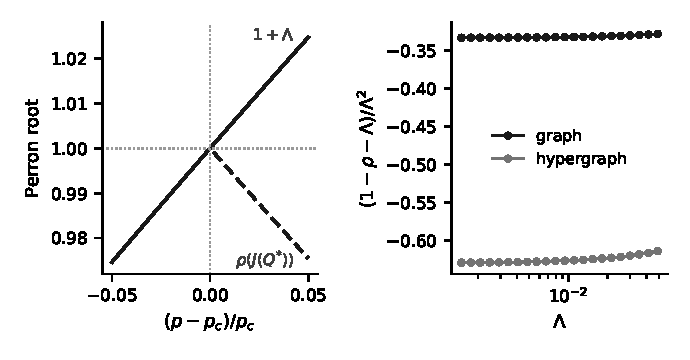
\includegraphics[width=\linewidth]{figs/fig-exchange.pdf}
\caption{\textbf{An exchange of stability.} Left: the Perron root of the
Jacobian at the trivial fixed point, $1+\Lambda$, and at the fixed point the map
reaches, for site percolation on a Poisson graph with $\ave{k}=3$. Where the
first passes through $1$ the second leaves it, at the same rate. Right: what is
left after the linear term, $(1-\rho-\Lambda)/\Lambda^{2}$, for that graph and
for a Poisson hypergraph with $\ave{k}=2$, $\ave{c}=3$. It settles at a constant,
so Eq.~\eqref{eq:exchange}'s remainder is quadratic; the constant is
model-dependent and the linear term is not. Generated by
\code{figs/\allowbreak statmech.\allowbreak py}.}
\label{fig:exchange}
\end{figure}

\paragraph{One diagnostic does not survive the move.} It is the natural thing
to reach for and it is wrong. The sign of the
leading eigenvalue does \emph{not} distinguish an order-preserving map from an
order-reversing one. The coupled core of a chygraph alternates between the up
and down roles of Eqs.~\eqref{eq:up} and~\eqref{eq:emitted}, so $J$ is a
non-negative matrix of period two, and Perron--Frobenius then places eigenvalues
at both $+\rho$ and $-\rho$. A negative leading eigenvalue is the geometry of
the chygraph, not a statement about the map.

The unambiguous test is the sign of the \emph{entries}: non-negative for a map
built from generating functions, non-positive for the hard-core maps of
Chapter~\ref{ch:hittingset}. That distinction decides which solver applies ---
plain iteration converges for one and oscillates forever for the other --- and
Chapter~\ref{ch:hittingset} turns on it.

\section{Free energy}
\label{sec:freeenergy}
\index{Bethe free energy|textbf}

A linear instability locates a transition only when the transition is
continuous. Chapter~\ref{ch:potts} met that limit at $q>2$,
Chapter~\ref{ch:giant} met it for interdependent networks and
Chapter~\ref{ch:epidemics} for threshold contagion, and
Chapter~\ref{ch:ising} will meet it again. In every case what is needed instead
is a free energy, so this chapter has to supply one.

The general Bethe free energy is Eq.~\eqref{eq:bethe-intro} with a complex in
place of a link: one term per complex, one per node, and one subtracted per
inclusion,
\[
  -\beta f=\sum_{a}\ln Z_{a}+\sum_{i}\ln Z_{i}
           -\sum_{(ia)}\ln Z_{ia},
\]
the last removing what the first two count twice. Parameterise the messages as
$\nu_{i\to a}(\sigma)\propto e^{h_{i\to a}\sigma}$ and
$\hat\nu_{a\to i}(\sigma)\propto e^{u_{a\to i}\sigma}$. The overlap term then
collapses, for a reason specific to this
parameterisation: $h_{i\to a}+u_{a\to i}$ is the \emph{same} full field $h_{i}$
for every complex $a$ containing $i$, so the overlaps do not depend on which
complex is being subtracted. What is left is one term per complex and $1-k_{i}$
per node,
\begin{equation}
  -\beta f=\sum_{l}n_{l}\ave{\ln Z^{(l)}_{a}}+\ave{(1-\kappa)\ln Z_{i}},
  \qquad
  n_{l}=\ave{\kappa_{l}}/c_{l},
  \label{eq:bethe}
\end{equation}
with $Z_{a}$ the exact partition function inside a complex --- the same
enumeration as Eq.~\eqref{eq:emitted}, reused --- and $Z_{i}=2\cosh h_{i}$. At
zero cavity field this closes,
\begin{equation}
  -\beta f_{\mathrm{para}}=\ln2+\sum_{l}\frac{\ave{\kappa_{l}}}{c_{l}}
    \ln\bigl(Z^{(l)}_{c}/2^{c_{l}}\bigr),
  \label{eq:para}
\end{equation}
$Z_{c}$ being the partition function of one isolated complex. For a graph
Eq.~\eqref{eq:para} is $\ln2+(\ave{k}/2)\ln\cosh\beta J$, which is the textbook
Bethe result and the check one wants.

Those weights --- $1$ on every complex, $1-k$ on every node --- are not chosen.
They are the M\"obius counting numbers of Chapter~\ref{ch:gbp}'s region graph in
the treelike case. Where complexes overlap, the counting and the free energy are
wrong in the same way, which is why Chapter~\ref{ch:overlap} can diagnose the
failure rather than merely observe it.

\section{The order parameter and the response}
\label{sec:response}
\index{magnetisation|textbf}
\index{susceptibility|textbf}
\index{critical amplitude}
\index{critical exponents}

Section~\ref{sec:branching} linearises the map and gives the transition.
Section~\ref{sec:freeenergy} gives the free energy. Differentiating that free
energy with respect to the external field $B$ of Eq.~\eqref{eq:up} gives the
two observables either side of the transition --- how large the order parameter
is below, how strongly the system answers a field above --- and neither step
uses what is inside a complex. So both are done here, once, and
Chapter~\ref{ch:ising} substitutes an interaction into them as it substitutes
one into Eq.~\eqref{eq:branch}.

\paragraph{The one-site partition function.} Take the definitions from $Z$,
Eq.~\eqref{eq:lnZ-intro}:
\begin{equation}
  m=\frac{1}{N}\frac{\partial\ln Z}{\partial(\beta B)}
   =-\frac{\partial f}{\partial B},
  \qquad
  \chi=\frac{\partial m}{\partial B}
      =-\frac{\partial^{2}f}{\partial B^{2}}.
  \label{eq:mfromZ}
\end{equation}
The object to differentiate is already in Eq.~\eqref{eq:bethe}. Cut one complex
out of the chygraph. On a treelike object the complexes that include it are
then independent, so each contributes the factor $e^{u_{b\to i}\sigma_{i}}$ it
emits, the external field contributes $e^{B\sigma_{i}}$, and
\begin{equation}
  Z_{i}=\sum_{\sigma=\pm1}e^{H_{i}\sigma}=2\cosh H_{i},
  \qquad
  H_{i}=B+\sum_{b\ni i}u_{b\to i}.
  \label{eq:Zi}
\end{equation}
This is Eq.~\eqref{eq:up} with nothing excluded, because nothing is being
passed onward: $H_{i}$ is the \emph{full} field where $h_{i\to a}$ is the cavity
field, and the difference between them is one term. Since the Bethe free energy
is stationary in the messages, differentiating Eq.~\eqref{eq:bethe} in $B$
picks up only this explicit dependence, and Eq.~\eqref{eq:mfromZ} gives
$m_{i}=\partial\ln Z_{i}/\partial B=\tanh H_{i}$.

Over an ensemble the substitution of Sec.~\ref{sec:substitution} applies to
$H$ as it applied to $h$. The law of the full field at a layer-$l$ complex is
Eq.~\eqref{eq:ensemblemap} with the \emph{ordinary} chy-degree in place of the
excess, since no inclusion is being discounted, so
\begin{equation}
  R^{l}=\delta_{B}\ast\Bigl(\ast_{k}\,\Phi^{l}_{k}\!\ast\,Q^{lk}\Bigr),
  \qquad
  m_{l}=\int\tanh(H)\,\mathrm{d}R^{l}(H).
  \label{eq:orderparam}
\end{equation}
The order parameter is one more convolution and not a new object. Everything
below is Eq.~\eqref{eq:orderparam} evaluated: at $B=0$ below the transition,
and differentiated once more at $B\to0$ above it.

\paragraph{The response.} Above the transition every message is $O(B)$, so
the down step is its linearisation Eq.~\eqref{eq:uprime} and the up step
Eq.~\eqref{eq:up} adds the field at the complex. Write $\hat\chi_{l}$ for the
mean cavity field sent into a layer-$l$ complex, divided by $B$. A complex
reached through a layer-$l$ inclusion still belongs to $\ave{\kbar}_{l}$ further
layer-$l$ complexes and $\ave{\kappa}_{k}$ layer-$k$ complexes for $k\ne l$,
each of which delivers $\ave{\sbar u'}_{k}$ per unit field --- which is
Eq.~\eqref{eq:branch} entry by entry. So
\begin{equation}
  \hat\chi_{l}=1+\sum_{k}B_{lk}\,\hat\chi_{k}.
  \label{eq:chicav}
\end{equation}
By Eq.~\eqref{eq:Zi} the full field counts the ordinary chy-degree instead of
the excess, and $m\simeq\ave{H}$ at small field, so Eq.~\eqref{eq:mfromZ} gives
\begin{equation}
  \chi=1+\sum_{l}w_{l}\,\hat\chi_{l},
  \qquad
  w_{l}=\ave{\kappa}_{l}\ave{\sbar u'}_{l}.
  \label{eq:chi}
\end{equation}
Equation~\eqref{eq:chicav} is $\hat\chi=(I-B)^{-1}\mathbf{1}$, so $\chi$
diverges exactly where $\det(I-B)$ vanishes --- which is Eq.~\eqref{eq:det}.
The condition that locates the transition and the divergence of the response
are one statement, and neither had to be assumed of the other.

Equation~\eqref{eq:chi} is general in everything Eq.~\eqref{eq:branch} is
general in, and for the same reason: only the linearisation entered it. Any
interaction inside a complex, through $u'$ alone; any distribution of
cardinalities within a layer, through the size-biased $\ave{\sbar u'}_{l}$ of
Eq.~\eqref{eq:sbaru}; any chy-degree distribution; any number of layers. The
size-biasing is not decoration here either. For the $3$-and-$5$ layer of
Sec.~\ref{sec:branching}, splitting it into one layer per cardinality returns
the same $\chi$ to machine precision and substituting its mean cardinality does
not, by $14.6$ per cent at $1.5\,T_{c}$ --- the same failure that moved
$T_{c}$ by $10.1$ per cent there.

Since $\det(I-B)$ vanishes linearly in $T-T_{c}$ for any interior that can be
enumerated, the exponent is $\gamma=1$:
\begin{equation}
  \chi\simeq\frac{A_{\chi}}{T/T_{c}-1},
  \qquad
  A_{\chi}=\frac{(w\cdot r)(\ell\cdot\mathbf{1})}
                {T_{c}\,\bigl|\mathrm{d}\lambda/\mathrm{d}T\bigr|_{T_{c}}},
  \label{eq:chiamp}
\end{equation}
with $\lambda$ the Perron root of $B$ and $r$, $\ell$ its right and left Perron
vectors normalised so that $\ell\cdot r=1$ --- the same vectors
Sec.~\ref{sec:amplitude} needed for percolation, doing the same job.

\paragraph{The order parameter, and where it closes.} Below the transition the
response is not the question and the shape of $R^{l}$ is. In general it has to
be carried, which is the population dynamics of Sec.~\ref{sec:substitution}. It
collapses to a point mass exactly when every message on a layer is one number,
and that needs two things: a whole-number chy-degree, so that every complex of
a layer has the same number of neighbours, and one cardinality per layer, so
that they all emit the same field. Call such a chygraph \emph{regular}. Writing
$\bar u_{k}(h)$ for the field a layer-$k$ complex emits when all $c_{k}-1$
incoming fields equal $h$, Eqs.~\eqref{eq:up} and~\eqref{eq:orderparam} become
\begin{equation}
  h_{l}=B+\sum_{k}\bigl(\kappa_{k}-\delta_{kl}\bigr)\,\bar u_{k}(h_{k}),
  \qquad
  m=\tanh\Bigl(B+\sum_{k}\kappa_{k}\,\bar u_{k}(h_{k})\Bigr),
  \label{eq:magclosure}
\end{equation}
$L$ scalars and no population --- and $m$ without a layer index is the
magnetisation, where $m$ with one would be a layer, which is why the sums here
run over $k$. The Kronecker delta is the excess bracket of
Sec.~\ref{sec:map} once more, and the difference between the two lines is the
difference between $h$ and $H$ in Eq.~\eqref{eq:Zi}.

For the amplitude, expand. Whatever the interior, it is odd under a spin flip,
so $\bar u_{k}(h)=a^{(k)}_{1}h+a^{(k)}_{3}h^{3}+O(h^{5})$, and both
coefficients are cumulants of one quantity. Writing $S$ for the total spin of
the other $c-1$ members under the Gibbs weight of the isolated complex with the
entered member held at $+1$, spin-flip symmetry makes $\bar{Z}(-1)$ at $h$ equal
$\bar{Z}(+1)$ at $-h$, so with $g$ the cumulant generating function of $S$ the emitted
field is $\bar u(h)=[g(h)-g(-h)]/2$ and
\begin{equation}
  a_{1}=\ave{S},
  \qquad
  a_{3}=\tfrac{1}{6}\,\kappa_{3}(S).
  \label{eq:a1a3}
\end{equation}
The first is $\ave{\sbar u'}$, the transmission Eq.~\eqref{eq:branch} already
needs, so the amplitude costs one further odd cumulant of a sum that has been
computed anyway --- which is the same accounting Chapter~\ref{ch:giant} found
for percolation, where the threshold took first moments and the amplitude took
one order more.

Putting $h=\epsilon r$ along the Perron direction and projecting on $\ell$
annihilates the linear term and leaves $\epsilon^{2}=(\lambda-1)/D$ with
$D=-\sum_{lk}\ell_{l}(\kappa_{k}-\delta_{kl})a^{(k)}_{3}r_{k}^{3}$, positive
whenever the interior saturates. Since $m\simeq(w\cdot r)\,\epsilon$ and
$\lambda-1$ vanishes linearly in $T_{c}-T$, the exponent is $\beta=1/2$ and
\begin{equation}
  m\simeq A_{m}\bigl(1-T/T_{c}\bigr)^{1/2},
  \qquad
  A_{m}=(w\cdot r)\sqrt{
    \frac{T_{c}\,\bigl|\mathrm{d}\lambda/\mathrm{d}T\bigr|_{T_{c}}}{D}}.
  \label{eq:magamp}
\end{equation}
Both amplitudes are built from the same Perron data; the response needs
$\lambda$ and its slope, and the order parameter needs $a_{3}$ as well.

\paragraph{One layer, three interiors.} Figure~\ref{fig:response} is the pair
of them over a family in which the interior is the only thing that moves: one
clique layer of cardinality $c$ at chy-degree $\kappa$, with $\kappa(c-1)=6$
held fixed, so that every member has six neighbours and the same degree
distribution whatever $c$ is. Raising the cardinality lowers $T_{c}$ ---
$4.9326$, $4.7209$, $4.4044$ --- and raises both amplitudes, $A_{m}$ from
$2.0926$ to $2.4869$ and $A_{\chi}$ from $1.2332$ to $1.5862$.
Chapter~\ref{ch:ising} reads the first two members of that family as a
statement about clustering and measures what they cost against a Monte Carlo;
here they are three substitutions into Eqs.~\eqref{eq:chi}
and~\eqref{eq:magclosure} with nothing else changed.

\begin{figure}[t]
\centering
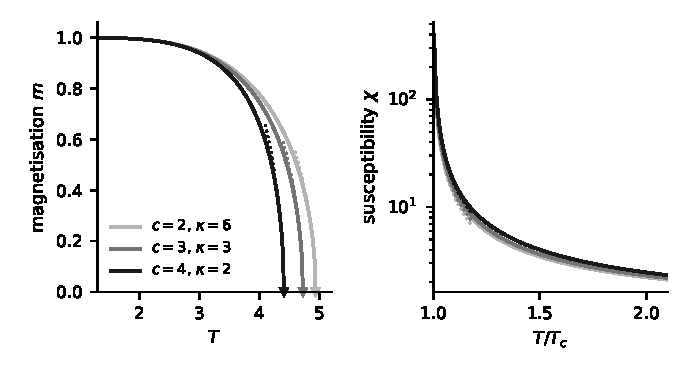
\includegraphics[width=\linewidth]{figs/fig-response.pdf}
\caption{\textbf{One formula, three interiors.} A single clique layer of
cardinality $c$ at chy-degree $\kappa$, with $\kappa(c-1)=6$ held fixed, so
every member has six neighbours either way and only what is inside a complex
differs. Left: the order parameter from Eq.~\eqref{eq:magclosure} in absolute
temperature, with the square-root asymptote Eq.~\eqref{eq:magamp} dotted and
each $T_{c}$ marked; it falls as the cardinality rises. Right: the response
from Eq.~\eqref{eq:chi} against reduced temperature, with the $\gamma=1$
asymptote Eq.~\eqref{eq:chiamp} dotted. Generated by
\code{figs/\allowbreak statmech.\allowbreak py}.}
\label{fig:response}
\end{figure}

\paragraph{What each of the two requires.} They are not equally general, and
the difference is the shape of the measure. Equation~\eqref{eq:chi} needs only
the linearisation, so it holds wherever Eq.~\eqref{eq:branch} does.
Equation~\eqref{eq:magclosure} needs the measure to be a point mass, so a
Poisson chy-degree, a fractional one, or a layer mixing cardinalities all leave
it: those carry a distribution of fields, the mean cardinality is not a summary
of one, and the route is the population. \code{Chygraph.\allowbreak
magnetisation} refuses such a structure rather than returning a number for it.

\section{The free energy from replicas}
\label{sec:replicas-chy}
\index{replica method|textbf}
\index{functional order parameter|textbf}
\index{Bethe free energy}

Sections~\ref{sec:freeenergy} and~\ref{sec:response} took the Bethe free energy
as given and differentiated it. It can instead be derived, from
Eq.~\eqref{eq:Z-intro} and nothing else, and the derivation is worth having for
what comes with it rather than for the free energy, which it returns unchanged.
It produces Eq.~\eqref{eq:bethe}'s counting numbers instead of assuming them.
It produces the two steps of Sec.~\ref{sec:twosteps}, excess bracket included,
as a stationarity condition instead of as bookkeeping put in by hand. And it
defines an order parameter \emph{before} any assumption about the number of
states, which is the object Sec.~\ref{sec:onestep} then breaks the symmetry of.

The calculation is \citet{leone2002}'s for a graph and
\citet{vazquez2003vw}'s with degree correlations, carried to a chygraph. The
formalism is \citet{mezard1987}; the diluted case in the form used here is
\citet{franz2003}.

One note on letters. In this section $n$ is the number of replicas and
$r=1,\dots,n$ indexes them, which is the only place in the book either does
that job; $\vec\sigma_{i}=(\sigma^{1}_{i},\dots,\sigma^{n}_{i})$ collects the
$n$ copies of the variable at atom $i$.

\paragraph{The object to average.} Take one atom layer and $L$ complex layers,
layer $l$ carrying cardinality $c_{l}$ and interior weight
$\chi_{l}=e^{-\beta H_{l}}$ --- the same $-\beta H$ Eq.~\eqref{eq:emitted} sums.
Then Eq.~\eqref{eq:Z-intro} reads
\begin{equation}
  Z=\sum_{\{\sigma\}}\ \prod_{i}e^{\beta B\sigma_{i}}
    \prod_{l}\prod_{a\in l}\chi_{l}\bigl(\{\sigma_{j}\}_{j\in a}\bigr),
  \label{eq:Zchy}
\end{equation}
and the free energy is $-\beta f=\overline{\ln Z}/N$, the bar an average over
which atoms each complex holds. That average is what the replica identity of
Sec.~\ref{sec:replicas} is for: $\overline{\ln Z}=\lim_{n\to0}
(\overline{Z^{n}}-1)/n$, with
\begin{equation}
  \overline{Z^{n}}=\sum_{\{\vec\sigma\}}\prod_{i}
    e^{\beta B\sum_{r}\sigma^{r}_{i}}\ \
    \overline{\prod_{l}\prod_{a\in l}\prod_{r}
      \chi_{l}\bigl(\{\sigma^{r}_{j}\}_{j\in a}\bigr)}.
  \label{eq:Zn}
\end{equation}
The chy-degrees are prescribed, so the average carries one constraint per atom
per layer, written in the integral form
$\delta\bigl(\sum_{a\in l}\alpha_{ia}-\kappa^{l}_{i}\bigr)
=\int\frac{\mathrm{d}\psi^{l}_{i}}{2\pi}
 e^{\mathrm{i}(\sum_{a\in l}\alpha_{ia}-\kappa^{l}_{i})\psi^{l}_{i}}$
with $\alpha$ the chy-adjacency matrix of Eq.~\eqref{eq:alpha}. This is the one
place a chygraph costs more than a graph: an edge is a pair by construction, so
a graph needs this constraint once, while a complex has a cardinality of its own
and needs it on both margins of $\alpha$.

\paragraph{The order parameter.} Tracing over the variables and integrating out
the $\psi$'s leaves everything expressed through one function per layer,
\begin{equation}
  \rho_{l}(\vec\sigma)=\frac{1}{N}\sum_{i}
     \delta_{\vec\sigma,\vec\sigma_{i}}\ e^{\mathrm{i}\psi^{l}_{i}},
  \label{eq:rhochy}
\end{equation}
and its conjugate $\hat\rho_{l}(\vec\sigma)$. It is a distribution over the
$2^{n}$ replica states, resolved by layer, and it is a \emph{functional} order
parameter: not a number, and not yet a field. Nothing has been assumed about it.
With
\begin{equation}
  \Xi_{l}[\rho]=\!\!\sum_{\vec\sigma_{1}\dots\vec\sigma_{c_{l}}}\
    \prod_{j=1}^{c_{l}}\rho_{l}(\vec\sigma_{j})
    \prod_{r}\chi_{l}\bigl(\sigma^{r}_{1},\dots,\sigma^{r}_{c_{l}}\bigr)
  \label{eq:Xichy}
\end{equation}
the interior sum in replica space, $\overline{Z^{n}}=\int\prod_{l,\vec\sigma}
\mathrm{d}\rho_{l}\,\mathrm{d}\hat\rho_{l}\ e^{-nNF}$ with
\begin{equation}
  \begin{aligned}
  -nF=&-\sum_{l}\ave{\kappa_{l}}\sum_{\vec\sigma}
        \rho_{l}(\vec\sigma)\hat\rho_{l}(\vec\sigma)\\
      &+\Bigl\langle\ln\sum_{\vec\sigma}e^{\beta B\sum_{r}\sigma^{r}}
        \prod_{l}\hat\rho_{l}(\vec\sigma)^{\kappa_{l}}\Bigr\rangle
       +\sum_{l}\frac{\ave{\kappa_{l}}}{c_{l}}\,\Xi_{l}[\rho],
  \end{aligned}
  \label{eq:Fchy}
\end{equation}
additive constants dropped.

\paragraph{What the three terms are.} They are one per complex, one per atom and
one subtracted per inclusion --- which is Sec.~\ref{sec:freeenergy}'s
un-collapsed free energy, term for term. The complex term carries
$\ave{\kappa_{l}}/c_{l}$, which is Eq.~\eqref{eq:bethe}'s $n_{l}$: a chygraph
has that many layer-$l$ complexes per atom. The inclusion term carries
$\ave{\kappa_{l}}$, one per inclusion. So Eq.~\eqref{eq:bethe}'s counting
numbers are not a choice made to make a tree work. They are the structure of
Eq.~\eqref{eq:Fchy}, and they were already the M\"obius numbers of
Chapter~\ref{ch:gbp}'s region graph. Three routes, one set of weights.

\paragraph{The saddle point is the two steps.} Setting the variations of
Eq.~\eqref{eq:Fchy} to zero gives
\begin{align}
  \hat\rho_{l}(\vec\sigma)&=\!\!\sum_{\vec\sigma_{2}\dots\vec\sigma_{c_{l}}}
    \prod_{j=2}^{c_{l}}\rho_{l}(\vec\sigma_{j})
    \prod_{r}\chi_{l}\bigl(\sigma^{r},\sigma^{r}_{2},\dots,
      \sigma^{r}_{c_{l}}\bigr),\label{eq:saddledown}\\
  \rho_{l}(\vec\sigma)&=\Bigl\langle\frac{\kappa_{l}}{\ave{\kappa_{l}}}\,
    \frac{e^{\beta B\sum_{r}\sigma^{r}}\hat\rho_{l}(\vec\sigma)^{\kappa_{l}-1}
          \prod_{m\ne l}\hat\rho_{m}(\vec\sigma)^{\kappa_{m}}}
         {\sum_{\vec\sigma'}e^{\beta B\sum_{r}\sigma'^{r}}
          \prod_{m}\hat\rho_{m}(\vec\sigma')^{\kappa_{m}}}\Bigr\rangle.
  \label{eq:saddleup}
\end{align}
Read them against Sec.~\ref{sec:twosteps}. Equation~\eqref{eq:saddledown} is the
down step: a complex reports what its other $c_{l}-1$ members do, summed over
its interior exactly. Equation~\eqref{eq:saddleup} is the up step, and it
carries two things that Sec.~\ref{sec:map} put in by hand. The weight
$\kappa_{l}/\ave{\kappa_{l}}$ is the size-biasing of
Sec.~\ref{sec:branching} --- a complex is reached in proportion to how many
inclusions it has. And the exponent is $\kappa_{l}-1$ in the layer arrived
through and $\kappa_{m}$ in every other, which is the excess bracket
$[\bar\Phi]_{k=m}$ of Fig.~\ref{fig:themap}. Neither was an assumption. Both
are what stationarity returns.

\paragraph{Replica symmetry, and Eq.~\eqref{eq:bethe}.} Write
$\nu_{h}(\sigma)$ for the normalised one-site law that a message $h$ stands
for: $e^{h\sigma}/2\cosh h$ for an Ising spin, a distribution over $q$ colours
in Chapter~\ref{ch:colouring}, a warning in
Chapter~\ref{ch:satisfiability}. What a message \emph{is} is the only thing
that changes from model to model, and Sec.~\ref{sec:onestep} is where it decides
what the next step costs. The replica-symmetric ansatz is then that a replica
state is a superposition of product states weighted by one message,
\begin{equation}
  \rho_{l}(\vec\sigma)=\!\int\!\mathrm{d}h\,P_{l}(h)
    \prod_{r}\nu_{h}(\sigma^{r}),
  \qquad
  \hat\rho_{l}(\vec\sigma)=\!\int\!\mathrm{d}u\,Q_{l}(u)
    \prod_{r}\nu_{u}(\sigma^{r}),
  \label{eq:rsansatz}
\end{equation}
which is where a message first enters the calculation --- and it enters as an
ansatz, not as a definition. Substituting Eq.~\eqref{eq:rsansatz} into
Eq.~\eqref{eq:saddledown} makes $Q_{l}$ the law of the field a complex emits
when its other members carry fields drawn from $P_{l}$, and the emitted field is
Eq.~\eqref{eq:emitted}. Substituting into Eq.~\eqref{eq:saddleup} makes $P_{l}$
the law of $B$ plus the fields arriving from the other complexes, which is the
convolution Eq.~\eqref{eq:ensemblemap}. Substituting into Eq.~\eqref{eq:Fchy}
returns Eq.~\eqref{eq:bethe}. So the whole of this chapter up to
Sec.~\ref{sec:response} is Eq.~\eqref{eq:Fchy} under one ansatz, and at
$c_{l}=2$ and one layer it is \citeauthor{leone2002}'s graph result.

\paragraph{The stability line, derived.} Expanding Eq.~\eqref{eq:Fchy} to second
order about the replica-symmetric saddle splits the fluctuations into sectors
that do not mix, classified by how they transform under permutations of the
replicas, and the one that goes unstable first is the \emph{replicon}. Its
eigenvalue is Eq.~\eqref{eq:branch} with $u'$ replaced by $u'^{2}$, which is the
elementwise reweighting of Eq.~\eqref{eq:reweight} and so
Sec.~\ref{sec:atline}'s de~Almeida--Thouless line. That section reaches the same
condition from the argument that a perturbation of random sign is transmitted
with $u'$ and its effect measured by squaring. The Hessian route is the one that
would establish it rather than motivate it, and the sectors are named here
without being computed.

\paragraph{What this does not do.} It does not make one-step replica symmetry
breaking cheap. Equation~\eqref{eq:Fchy} is the object a one-step ansatz acts
on, and Sec.~\ref{sec:onestep} writes that ansatz down; what neither supplies is
a solution where the message is a real field rather than a warning.
Section~\ref{sec:hsrsb} is where that is met and declined, and
Sec.~\ref{sec:notdone} lists it. The derivation moves the difficulty from
\emph{what object to write} to \emph{how to solve it}, which is progress of a
limited kind and is worth saying plainly.

\section{One step of replica symmetry breaking}
\label{sec:onestep}
\index{replica symmetry breaking!one-step, on a chygraph|textbf}
\index{survey propagation|textbf}
\index{complexity|textbf}
\index{Parisi parameter}

Everything above carries one field per inclusion, and that is an assumption
about the solution space and not a convention. A message can be a field because
there is one thing to say. Where the space shatters into exponentially many
clusters --- as it does for every hard constraint in Part~III, at a density
below the one where solutions disappear --- each cluster would send its own
field along the same inclusion, and no single field is right for all of them.

\paragraph{The substitution, one level up.} The repair is
Sec.~\ref{sec:substitution}'s move made a second time, and it is worth being
exact about the difference, because the two produce the same kind of object for
different reasons. There, a field became a \emph{measure over fields} to pass
from one realisation to an ensemble: the spread in $P^{ml}$ is variation across
the graphs in the ensemble. Here a field becomes a measure over fields at
\emph{fixed} realisation: the spread is variation across the clusters of one
graph. That object is a \emph{survey},
\begin{equation}
  S_{i\to a}(h)=\text{the law, over clusters, of the field }i\text{ sends }a,
  \label{eq:survey}
\end{equation}
and the ensemble version stacks on top of it --- a distribution over surveys,
which is what a population dynamics stores and why the populations of
Chapters~\ref{ch:colouring} and~\ref{ch:satisfiability} are populations of
distributions rather than of numbers.

What does \emph{not} change is the recursion. The up step of
Sec.~\ref{sec:upstep} still adds the incoming fields; the down step of
Sec.~\ref{sec:downstep} still enumerates the interior of a complex exactly.
Both now act on surveys rather than on fields, and each combination is
reweighted by $e^{-m\Delta F}$, with $\Delta F$ the free-energy shift the
combination costs and $m$ the Parisi parameter --- the one place in this chapter
where $m$ is not a layer index. The index structure --- layers,
the direction of arrival, the discounting of the inclusion one came in by ---
survives this exactly as it survived the first substitution, and for the same
reason: none of it was ever about what the message contained.

\paragraph{Counting the clusters.} A branch of the survey recursion appearing is
not a threshold. What decides whether solutions still exist is how many clusters
there are, and that is a free energy rather than a branch. Reweighting
Eq.~\eqref{eq:bethe} at $m=0$ turns the Bethe expression into a count of
clusters --- the \emph{complexity}
\begin{equation}
  \Sigma=\ave{\ln Z_{i}}
        +\sum_{l}\frac{\ave{\kappa_{l}}}{c_{l}}\ave{\ln Z^{(l)}_{a}}
        -\sum_{l}\ave{\kappa_{l}}\ave{\ln Z^{(l)}_{ia}},
  \label{eq:sigmagen}
\end{equation}
the same three objects the free energy is built from --- a node, a complex, an
inclusion --- evaluated on surveys instead of on fields, with
$\ave{\kappa_{l}}/c_{l}$ complexes and $\ave{\kappa_{l}}$ inclusions per node in
layer $l$. Where $\Sigma$
falls to zero the clusters have run out, and that is the threshold. Note that
the overlap term does not collapse here as it did in
Eq.~\eqref{eq:bethe}: the argument that made $h_{i\to a}+u_{a\to i}$ the same
full field for every complex is an argument about one field, and the
reweighting is what breaks it. Three terms rather than two is the whole
bookkeeping cost of the step.

\paragraph{The same step, on the replica order parameter.}
Equation~\eqref{eq:survey} is a definition, and
Sec.~\ref{sec:replicas-chy} says what it is an ansatz \emph{for}. Replica
symmetry was Eq.~\eqref{eq:rsansatz}, every replica carrying the same field.
Break the $n$ replicas into $n/m$ blocks of $m$, let the field be common within
a block and drawn from a distribution across blocks, and
Eq.~\eqref{eq:rhochy} becomes
\begin{equation}
  \rho_{l}(\vec\sigma)=\int\!\mathcal{D}Q\ \mathcal{P}_{l}[Q]
    \prod_{\text{blocks}}\Bigl[\int\!\mathrm{d}h\,Q(h)
      \prod_{r\in\text{block}}\nu_{h}(\sigma^{r})\Bigr],
  \label{eq:rsbansatz}
\end{equation}
with $Q$ the survey of Eq.~\eqref{eq:survey} and $\mathcal{P}_{l}$ the law over
surveys that the ensemble carries. Two things then follow instead of being
imposed. The reweighting $e^{-m\Delta F}$ is what the sum over blocks produces,
so $m$ is a block size rather than a parameter added to taste. And substituting
Eq.~\eqref{eq:rsbansatz} into Eq.~\eqref{eq:Fchy} returns
Eq.~\eqref{eq:sigmagen}, which also says why the overlap term does not collapse
here as it did in Eq.~\eqref{eq:bethe}: that collapse used one field per
inclusion, and Eq.~\eqref{eq:rsbansatz} carries a distribution of them.

\paragraph{Two transitions, not one.} The survey recursion therefore carries two
pieces of information and they should not be confused. The trivial survey ---
every cluster sending the same field, which is the replica-symmetric solution
--- is a fixed point at any density. Where a second branch appears, the state
space has \emph{shattered}: there are now many clusters, and that density is the
dynamical or clustering transition. Where $\Sigma$ then falls to zero the
clusters have run out and solutions cease to exist. Solutions survive past the
first and not past the second, and the gap between them is the r\'egime survey
propagation was invented for.

The first of the two is sometimes reachable without a survey at all. Where the
shattering coincides with the appearance of a rigid structure, that structure
can be found by an ordinary percolation calculation of the kind Part~II
supplies: Chapter~\ref{ch:cover}'s core is exactly this, located by algebra
rather than by a population, and Chapter~\ref{ch:colouring} finds the same class
of point as the onset of its survey branch. The structural route is cheaper and
exact, and it is model-specific --- it says where clusters appear and nothing
about how many, which is what $\Sigma$ is for.

\paragraph{$m=0$, and what it buys.} Setting $m=0$ weights every cluster
equally, which is the right choice for counting clusters of \emph{zero-energy}
solutions and the wrong one for anything finer. There the reweighting is trivial
except at one place --- a combination that contradicts itself gets weight zero
and is discarded --- and the recursion reduces to \emph{survey propagation}.
This is the form Part~III uses, in Secs.~\ref{sec:colouring-sp}
and~\ref{sec:sat-sp}, and Eq.~\eqref{eq:sigmagen} is the equation both of those
sections instantiate. What $m=0$ does not reach is the condensation and rigidity
transitions, which need $m\ne0$ and are outside this book.

\paragraph{What the step costs.} Three things, and the last is the one a
chygraph makes visible.

\emph{The scalar closure goes.} Under replica symmetry a hard-field message is
present or absent and its mean is all of it, so a single number closes the
recursion over an ensemble. A survey is a continuous variable and its
\emph{spread} enters the next update; solving for the mean alone is not an
approximation but a different and wrong calculation.
Section~\ref{sec:sat-sp} measures the error at $28$ per cent.

\emph{The alphabet decides whether it is affordable at all.} Where the
underlying message is a warning --- present or absent, or one of a few discrete
states, which is what a hard constraint at zero temperature produces --- a
survey is a distribution over a finite alphabet and can be carried as a handful
of numbers. Where the message is a real field, a survey is a distribution over
distributions, and the population becomes a population of populations. That is
the line this book does not cross: Chapters~\ref{ch:colouring}
and~\ref{ch:satisfiability} are the two problems whose messages are warnings,
and Sec.~\ref{sec:hsrsb} is where the heavier object is met and declined.

\emph{The interior sum grows, by an amount the model decides.} The cost of
Eq.~\eqref{eq:emitted} was $2^{c}$ and depended on nothing but cardinality. The
cost of the same sum on surveys depends on how much one complex can transmit at
once. Where a complex can force at most one thing --- the hypergraph rule of
Sec.~\ref{sec:colouring-sp-chy}, a $k$-SAT clause --- the message is the same
kind of object it was at $c=2$ and cardinality enters through a single scalar.
Where a complex can force up to $c-1$ things at once, as proper colouring can,
the message becomes a \emph{set} and the interior must be summed over subsets;
Sec.~\ref{sec:colouring-cq} is that calculation and the extra work is real.
The distinction has no counterpart on a graph, where a complex with two members
has no room to force two things at once --- one more instance of the pattern
Sec.~\ref{sec:twoconstraints-col} collects, that cardinality two is degenerate
and a good deal of what reads as general theory is an artefact of working
there.

\section{What the scheme assumes}
\label{sec:assumes}
\index{replica symmetry breaking}

Three assumptions, of quite different weights.

\emph{Treelikeness, at the level of atoms.} Equation~\eqref{eq:up} treats an
atom's complexes as independent, which is exact when they meet in at most one
atom. This is Sec.~\ref{sec:treelike}'s condition, and it is the one
Chapter~\ref{ch:overlap} takes up: what happens when the cliques of a real
network share edges rather than vertices.

\emph{Replica symmetry.} One field per inclusion presumes a single pure state.
Equation~\eqref{eq:rsansatz} is that presumption written down, and
Sec.~\ref{sec:replicas-chy} is where it can be seen as an ansatz on something
more general rather than as the definition of a message.
Section~\ref{sec:onestep} is what replaces it where the state space shatters,
and it is a repair rather than a limit --- but a partial one, since it is
carried out at $m=0$ throughout this book.
Chapter~\ref{ch:hittingset} is where the assumption first becomes unavoidable,
and it is also where the diagnostic of Sec.~\ref{sec:fixedpoint} is needed.

\emph{An enumerable interior.} Equation~\eqref{eq:emitted} costs $2^{c}$. For
the motifs one finds in data that is nothing, and for a complex of thirty
members it is fatal. The formalism does not degrade gracefully here: it either
enumerates the interior or it does not apply. Cardinality is the one parameter
of a chygraph that has a hard ceiling, and Sec.~\ref{sec:onestep} lowers it
again wherever the interior has to be summed over surveys rather than fields.

\paragraph{A note on the numbers quoted.} Agreements reported in this book to
eight, ten or twelve digits are between two evaluations of the \emph{same}
analytic object --- a closed form against an enumeration, a symbolic derivative
against a numerical one. They establish that the implementation is faithful, not
that the physics is right. Where something is tested against something outside
the formalism it is said so: the Monte Carlo of Chapter~\ref{ch:ising}, the
leaf-removal simulations of Chapters~\ref{ch:cover} and~\ref{ch:overlap}, the
configuration-model simulations of Chapter~\ref{ch:giant}, and published values
where they exist. The distinction matters most in exactly this chapter, which
has nothing in it to compare against experiment and everything in it to get
wrong.

\section{Checks}
\label{sec:statmech-checks}

\checkhead{Known results}
Equation~\eqref{eq:bethe} is evaluated on populations produced by iterating
Eq.~\eqref{eq:ensemblemap} itself, then compared with the closed form of
Eq.~\eqref{eq:para} and with the textbook Bethe expression
$\ln2+(\ave{k}/2)\ln\cosh\beta J$ for a graph. The three agree to ten digits, and the
outermost of them is a simulation of the distributions rather than an evaluation
of a formula.

\checkhead{New results}
Nothing else in this chapter has appeared elsewhere, so the checks are against
independent evaluations of the same object.
Section~\ref{sec:response}'s two observables are checked as limits rather than
at a point: $m/(1-T/T_{c})^{1/2}$ against $A_{m}$ and $\chi\,(T/T_{c}-1)$
against $A_{\chi}$, over three decades of reduced temperature and on five
structures, agreeing to a part in a thousand at the closest, so the exponents
$\beta=1/2$ and $\gamma=1$ are measured rather than asserted. That $1/\chi$
vanishes exactly where $\det(I-B)$ does is checked on four layer lists rather
than argued from Eq.~\eqref{eq:chicav}. Equation~\eqref{eq:mfromZ} asserts one
thing the derivation does not enforce, that the response is the field
derivative of the order parameter, and it is checked directly: the closed form
Eq.~\eqref{eq:chi} against a finite difference of Eq.~\eqref{eq:magclosure} in
the field, on four structures at three temperatures each, agreeing to five
digits --- the accuracy of the difference and not of either expression.
Equation~\eqref{eq:chi} is checked to be general in the cardinality
distribution by the two routes Eq.~\eqref{eq:sbaru} is: a mixed layer against
the same layer split into one layer per cardinality, agreeing to machine
precision at three temperatures, and against the mean-cardinality substitution,
which must not agree and does not, by $14.6$ per cent. That $u'$ is
Chapter~\ref{ch:potts}'s $\tau_{c}$ is checked directly: the symbolic
$q$-derivative of Sec.~\ref{sec:transmission}, evaluated at $q=2$ and rewritten
in $t=\tanh\beta J$, agrees with the independent enumeration behind
Eq.~\eqref{eq:emitted} for $c=2,3,4$ at every coupling tried, to machine
precision. Two chapters written from different starting points return one
number. Equation~\eqref{eq:sbaru} is checked by the two routes of
Sec.~\ref{sec:branching}: a mixed-cardinality layer against the same layer split into one
layer per cardinality, which must agree and do, to nine digits; and against the
mean-cardinality substitution, which must not agree and does not, by $10.1$ per cent.
Equation~\eqref{eq:LT} is checked against the numerical determinant of
Eq.~\eqref{eq:branch} at the critical coupling for Poisson and for regular
layers, so that the cross term is exercised in both the case where it vanishes
and the case where it does not. Equation~\eqref{eq:exchange} is checked by
taking the residual to zero along a sequence rather than at a point, with the
sequence stopped where rounding would begin to dominate; that qualification is
the difference between demonstrating an order and quoting a number that happens
to be small.

\checkhead{Partial results}
Equation~\eqref{eq:magclosure} holds only where the message measure is a point
mass, which needs a whole-number chy-degree and one cardinality per layer.
Everything else --- a Poisson layer, a fractional chy-degree, a layer mixing
cardinalities --- carries a distribution of fields and needs the population,
which is a sample and not a closed form; the routine refuses such a structure
rather than returning a number for it. Equation~\eqref{eq:chi} has no such
restriction, so the two are not equally general and the section says which is
which. Nothing in Sec.~\ref{sec:response} is tested against a simulation
here: Chapter~\ref{ch:ising} does that, on the two structures where the
closure applies and against a Monte Carlo that has never heard of a cavity
equation.
The agreements quoted above are between two evaluations of the same analytic
object, in the sense Sec.~\ref{sec:assumes} sets out. Nothing in this chapter is
tested against experiment or against an object built to violate its assumptions:
Sec.~\ref{sec:assumes}'s three --- treelikeness at the level of atoms, replica
symmetry, and an enumerable interior --- are assumed throughout and checked
nowhere here. The one-step scheme of Sec.~\ref{sec:onestep} is written at $m=0$
only.
Section~\ref{sec:replicas-chy} is a derivation and not a computation. It
returns Eq.~\eqref{eq:bethe}, which is checked above, and adds no number of its
own. The reductions it claims --- Eq.~\eqref{eq:saddledown} to
Eq.~\eqref{eq:emitted}, Eq.~\eqref{eq:saddleup} to
Eq.~\eqref{eq:ensemblemap}, and Eq.~\eqref{eq:Fchy} to Eq.~\eqref{eq:bethe}
under Eq.~\eqref{eq:rsansatz} --- are stated as algebra and are not
machine-checked, which is a weaker footing than the rest of the chapter stands
on. Equation~\eqref{eq:rsbansatz} is written and not solved.


% sources
% - the retired manuscript, Secs. II-III and supplement Secs. I-II
%   (git history, commit 5ebd892)

\chapter{Ising model}
\label{ch:ising}
\index{Ising model}

The Ising model is the first model through the machinery of
Chapter~\ref{ch:statmech}, worked end to end. Its results are new here, and
the published work it is checked against --- the Bethe critical temperature, and
the motif calculations of \citet{yoon2011} --- is cited where used. It comes first for two reasons:
its answer on a graph is already known, so every step can be checked against it;
and its result here is a sign that goes the other way from the obvious one.

Clustering \emph{lowers} the critical temperature at fixed degree, and it does
so even though a triangle transmits \emph{more} per traversal than a link does.
Both halves hold, and they pull in opposite directions.
Section~\ref{sec:magnetisation} substitutes the same interior into
Sec.~\ref{sec:response}'s magnetisation and susceptibility, where it closes
twice against textbook answers; Sec.~\ref{sec:clustering} is then the
accounting, on a null model where all three quantities are exact. There the two effects come apart: clustering
costs the transition temperature and buys a steeper rise out of it.
Section~\ref{sec:isingfive} runs the whole of it over the five structures of
Fig.~\ref{fig:mappings}, one paragraph each, where the accounting turns out to
matter more than the structure does.

\section{Spins inside complexes}
\label{sec:spins}

Put an Ising spin $\sigma_{i}=\pm1$ on every node, couple every pair inside
every complex, and write down the partition function the rest of the chapter
differentiates:
\begin{equation}
  \begin{aligned}
    \mathcal{H}&=-J\sum_{a}\ \sum_{\{i,j\}\subset a}\sigma_{i}\sigma_{j}
              \;-\;B\sum_{i}\sigma_{i},\\
    Z&=\sum_{\{\sigma\}}e^{-\beta\mathcal{H}},
    \qquad
    f=-\frac{1}{\beta N}\ln Z,
  \end{aligned}
  \label{eq:Hising}
\end{equation}
the first sum over complexes, the second over nodes, and $N$ the number of
nodes. A complex of cardinality $c$ therefore carries $\binom{c}{2}$ bonds,
and a graph is the case $c=2$ where each carries one. The external field $B$ is
zero except where Sec.~\ref{sec:response} differentiates $f$ with respect to
it; it is written $B$ rather than $h$ because $h$ is the cavity field of
Eq.~\eqref{eq:up}, the busiest symbol in Part~III, and because
Chapter~\ref{ch:introduction} introduced the field under that letter.
Where a $B$ carries two layer indices, or stands inside $\det(I-B)$, it is
the branching matrix of Eq.~\eqref{eq:branch} and not a field.

The Ising model on graph ensembles with prescribed motifs has been treated
directly \citep{yoon2011}; the point here is that no separate treatment is
needed. That is the entire model specification, and everything else is
Chapter~\ref{ch:statmech}: Eq.~\eqref{eq:emitted} with Eq.~\eqref{eq:Hising}
inside it gives $u'$, Eq.~\eqref{eq:branch} gives the transition, and squaring
$u'$ gives the de Almeida--Thouless line instead. The calculation is $L\times L$
linear algebra with an enumeration of size $2^{c}$ behind each entry, and
nothing about it had to be invented for this chapter.

\section{What a complex transmits}
\label{sec:transmits}
\index{transmission factor}

Writing $t=\tanh\beta J$, the interior sum gives
\begin{equation}
  \begin{aligned}
    c=2:&\quad u'=t,\\
    c=3:&\quad u'=t/(1-t+t^{2}),\\
    c=4:&\quad u'=(t+t^{3})/(1-2t+3t^{2}),
  \end{aligned}
  \label{eq:uclique}
\end{equation}
with no useful closed form beyond, but exact by enumeration at any cardinality
small enough to enumerate --- which is the same condition the rest of the
formalism already lives under.

By Eq.~\eqref{eq:emitted},
\[
  u'=\frac{\partial}{\partial h_{1}}\tfrac12\bigl[\ln Z(+)-\ln Z(-)\bigr]
     \bigg|_{h=0}
    =\tfrac12\Bigl[\ave{\sigma_{1}}_{+}-\ave{\sigma_{1}}_{-}\Bigr],
\]
the two averages taken inside the complex at zero cavity field with $\sigma_{0}$
held at $+1$ and at $-1$.

For $c=3$ with $a=\beta J$, the interior energy
$\sigma_{0}\sigma_{1}+\sigma_{0}\sigma_{2}+\sigma_{1}\sigma_{2}$ takes the value
$3$ on the one configuration where both others agree with $\sigma_{0}$, and
$-1$ on the other three. So
\[
  \ave{\sigma_{1}}_{+}=\frac{e^{3a}-e^{-a}}{e^{3a}+3e^{-a}}
                      =\frac{e^{4a}-1}{e^{4a}+3},
\]
and $\ave{\sigma_{1}}_{-}=-\ave{\sigma_{1}}_{+}$ by spin-flip symmetry. Hence
$u'=(e^{4a}-1)/(e^{4a}+3)$, and substituting $e^{2a}=(1+t)/(1-t)$,
\[
  u'=\frac{(1+t)^{2}-(1-t)^{2}}{(1+t)^{2}+3(1-t)^{2}}
    =\frac{4t}{4-4t+4t^{2}}=\frac{t}{1-t+t^{2}}.
\]
The same enumeration at $c=4$ gives the third line of
Eq.~\eqref{eq:uclique}, and beyond that the expressions stop being worth
writing down. \code{Chygraph.\allowbreak u\_\allowbreak prime} returns them, over
\code{ising.\allowbreak clique\_\allowbreak derivative} for the closed forms and
\code{cavity.\allowbreak cavity\_\allowbreak derivative} for the enumeration they
are checked against.

The first half of the chapter's result follows at once, and it is the intuitive
half. Since $t/(1-t+t^{2})>t$ on $0<t<1$, and $(t+t^{3})/(1-2t+3t^{2})$ is larger
still, \emph{a triangle transmits more to each of its members than an
independent edge does} (Fig.~\ref{fig:transmit}). The extra route --- round the
third corner --- is real, and it is precisely the loop that a tree-based
calculation on the underlying graph could not have kept.

\begin{figure}[t]
\centering
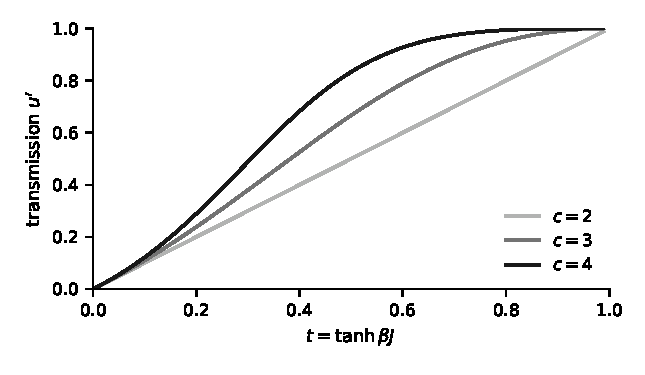
\includegraphics[width=0.88\linewidth]{figs/fig-transmit.pdf}
\caption{\textbf{More per traversal.} The transmission $u'$ of
Eq.~\eqref{eq:uclique} against $t=\tanh\beta J$. The $c=2$ curve is the
diagonal $u'=t$; larger complexes lie above it, because a member can be reached
around the inside of the complex as well as directly. At leading order in $t$
all three coincide, so the enhancement is $O(t^{2})$ --- which is why
Sec.~\ref{sec:clustering}'s effect decays with degree. Generated by
\code{figs/\allowbreak ising.\allowbreak py}.}
\label{fig:transmit}
\end{figure}

It would be natural to conclude that clustering favours order. It does not, and
Sec.~\ref{sec:clustering} is why.

\section{The critical temperature}
\label{sec:tc}
\index{critical temperature|textbf}

Substituting Eq.~\eqref{eq:uclique} into Eq.~\eqref{eq:branch} and turning the
handle, structure by structure.

On a graph the condition is
\begin{equation}
  \ave{\kbar}\,\tanh\beta J=1,
  \label{eq:tcgraph}
\end{equation}
which is Eq.~\eqref{eq:tc-intro} --- the textbook Bethe result, and the
reassurance one wants before trusting anything else in the chapter. It is also
Chapter~\ref{ch:potts}'s $\tau_{2}(2,v)\ave{\kbar}=1$, the same line reached
along a third route.

On a network of $c$-cliques it is $\ave{\kbar}(c-1)u'(c)=1$, and on a graph
with links and triangles it is Eq.~\eqref{eq:LT}. Neither needs a closed form to
be evaluated. At chy-degree two, a single clique layer gives Table~\ref{tab:cliquetc}.
\begin{table}[t]
\centering\small
\begin{tabular}{lccccc}
\hline\hline
$c$ & $2$ & $3$ & $4$ & $5$ & $6$\\
\hline
$\beta J_{c}$ & $0.5493$ & $0.2118$ & $0.1304$ & $0.0940$ & $0.0734$\\
AT line & $0.8814$ & $0.4024$ & $0.2670$ & $0.2015$ & $0.1625$\\
\hline\hline
\end{tabular}
\caption{\textbf{One clique layer at chy-degree two.} The critical coupling from $\ave{\kbar}(c-1)u'(c)=1$, and the de Almeida--Thouless coupling from the same condition with $u'$ replaced by $u'^{2}$, against cardinality. Generated by \code{figs/\allowbreak ising.\allowbreak py}.}
\label{tab:cliquetc}
\end{table}
with the second row anticipating Sec.~\ref{sec:atline}.

\paragraph{Over several layers.} Those are the one- and two-layer cases of one
formula, and it is worth having in general because three of
Fig.~\ref{fig:mappings}'s five structures carry more than one layer.
Equation~\eqref{eq:branch} puts $\ave{\kbar}_{m}$ on the diagonal and
$\ave{\kappa}_{m}$ off it and multiplies both by the same
$(c_{m}-1)u'(c_{m})$, so $B$ is a rank-one matrix plus a diagonal,
$B=\mathbf{1}v^{\!\top}+\mathrm{diag}(d)$ with
$v_{l}=\ave{\kappa}_{l}(c_{l}-1)u'(c_{l})$ and
$d_{l}=(\ave{\kbar}_{l}-\ave{\kappa}_{l})(c_{l}-1)u'(c_{l})$. A matrix of that
shape has a scalar determinant condition, so $\det(I-B)=0$ is
\begin{equation}
  \sum_{l}\frac{\ave{\kappa}_{l}(c_{l}-1)\,u'(c_{l})}
               {1-\bigl(\ave{\kbar}_{l}-\ave{\kappa}_{l}\bigr)(c_{l}-1)\,u'(c_{l})}
  =1,
  \label{eq:tcmulti}
\end{equation}
one term per layer and an eigenvalue problem no longer. At one layer the
$\ave{\kappa}$'s cancel and it is $\ave{\kbar}(c-1)u'(c)=1$, which is
Eq.~\eqref{eq:tcgraph} at $c=2$; at two layers, expanded, it is
Eq.~\eqref{eq:LT}. With Poisson layers every $\ave{\kbar}_{l}=\ave{\kappa}_{l}$,
every $d_{l}$ vanishes, and it flattens further to
$\sum_{l}\ave{\kappa}_{l}(c_{l}-1)u'(c_{l})=1$: the layers add, and nothing but
the sum survives.

\section{Magnetisation and susceptibility}
\label{sec:magnetisation}
\index{magnetisation}
\index{susceptibility}
\index{critical amplitude}

Section~\ref{sec:response} took the two observables either side of the
transition for an arbitrary interior: the order parameter
Eq.~\eqref{eq:magclosure} and the response Eq.~\eqref{eq:chi}, with the
exponents $\beta=1/2$ and $\gamma=1$ and the two amplitudes
Eqs.~\eqref{eq:magamp} and~\eqref{eq:chiamp}, in the same external field $B$
as Eq.~\eqref{eq:Hising}. Substituting the Ising interior into them is this
section, and it costs what substituting into Eq.~\eqref{eq:branch} cost in
Sec.~\ref{sec:tc}: an enumeration and nothing else.

\paragraph{What the interior supplies.} Equation~\eqref{eq:a1a3} asks for two
cumulants of the interior magnetisation $S$, and for the all-pairs clique they
are had from the same enumeration as Sec.~\ref{sec:transmits}. The first is
$a_{1}=(c-1)u'$ with $u'$ of Eq.~\eqref{eq:uclique}, so nothing new is computed
for it. The second has a closed form at $c=2$: expanding
$\bar u(h)=\mathrm{atanh}(t\tanh h)$ gives
\begin{equation}
  a_{3}=\tfrac{1}{3}\,t\,(t^{2}-1),
  \label{eq:a3edge}
\end{equation}
negative on $0<t<1$ because a bond saturates, which is the condition
Eq.~\eqref{eq:magamp} needs to have a continuous branch at all. Above $c=2$ it
is a number from the enumeration, as $u'$ is.

\paragraph{The susceptibility on a graph.} One layer at $c=2$ with $u'=t$
reduces Eq.~\eqref{eq:chi} to $\chi=1+\ave{k}t/(1-\ave{\kbar}t)$. For a
$k$-regular graph $\ave{\kbar}=k-1$ and this is
\begin{equation}
  \chi=\frac{1+t}{1-(k-1)t},
  \label{eq:chibethe}
\end{equation}
the Bethe-lattice susceptibility; for a Poisson degree, its own excess, it is
$\chi=1/(1-\ave{k}t)$. Both are textbook, and both come out of
Eq.~\eqref{eq:chi} without adjustment --- which is the reassurance this chapter
wants before trusting the same expression on a clique layer.
Equation~\eqref{eq:chiamp} then collapses to $A_{\chi}=T_{c}/(k-2)$.

\paragraph{The amplitude on a graph.} Equation~\eqref{eq:magamp} likewise
closes at $c=2$:
\begin{equation}
  A_{m}=\frac{k}{k-1}\sqrt{\frac{3(k-1)J}{T_{c}}},
  \label{eq:magampgraph}
\end{equation}
which returns $2.3548$ at $k=4$. As $k$ grows $T_{c}\to J(k-1)$ and
$A_{m}\to\sqrt3$, the Curie--Weiss amplitude of the fully connected magnet: the
second check from outside, and the one that says the machinery reduces to mean
field where it has to.

\section{Clustering lowers \texorpdfstring{$T_{c}$}{Tc}}
\label{sec:clustering}
\index{clustering!and the critical temperature|textbf}
\index{null model}

Equation~\eqref{eq:branch} carries a \emph{multiplicity} as well as a
transmission, and the two move in opposite directions. The accounting between
them is what follows.

Arrive at a degree-$n$ vertex of a graph along one of its links. Then $n-1$
further links branch away. Arrive at the same vertex through one of its $n/2$
triangles, and only $n-2$ branch --- because one of the two neighbours in the
triangle just traversed is already accounted for, its influence sitting inside
$u'$ rather than being counted again as a separate route.

More per branch, fewer branches. Which wins is arithmetic. At $n=4$ the two
conditions are $3t=1$ for links and $2u'_{\triangle}=1$ for triangles, so at the
link ensemble's critical coupling $t=1/3$ the triangle enhancement would have to
carry $u'$ from $1/3$ to $1/2$ to break even. It reaches
\begin{equation}
  u'_{\triangle}\bigl(t=\tfrac13\bigr)
    =\frac{1/3}{1-\tfrac13+\tfrac19}=\frac{3}{7},
\end{equation}
which is not enough. The lost branch wins, and the network of triangles needs to
be colder before it orders.

\paragraph{Against a null model that is actually matched.} The comparison has to
be stated carefully, and this book has said why in four places already ---
Secs.~\ref{sec:promoting}, \ref{sec:helporhurt}, \ref{sec:joint}
and~\ref{sec:epidemics-lessons}: naming what is held fixed is most of the work. The unambiguous null is regular. Take an
$n$-regular graph against a network of $n/2$ triangles per vertex. These have
identical degree distribution $p_{d}=\delta_{d,n}$, identically neutral degree
correlations, and the same number of edges per vertex. They differ in one thing
only: whether those edges close into triangles (Table~\ref{tab:trianglenull}).
\begin{table}[t]
\centering\small
\begin{tabular}{rrrr}
\hline\hline
$n$ & $T_{c}$ links & $T_{c}$ triangles & change\\
\hline
$4$ & $2.8854$ & $2.4853$ & $-13.9\%$\\
$6$ & $4.9326$ & $4.7209$ & $-4.3\%$\\
$8$ & $6.9521$ & $6.8052$ & $-2.1\%$\\
$10$ & $8.9628$ & $8.8498$ & $-1.3\%$\\
$20$ & $18.9824$ & $18.9296$ & $-0.3\%$\\
\hline\hline
\end{tabular}
\caption{\textbf{Clustering lowers $T_{c}$ at fixed degree.} An $n$-regular graph against a network of $n/2$ triangles per vertex: identical degree distribution, identically neutral degree correlations, the same number of edges per vertex, differing only in whether those edges close into triangles. The effect is largest at low degree and dies as $1/n^{2}$: the last column is $-1/(n-1)^{2}$ to within seven per cent from $n=6$ upward. Generated by \code{figs/\allowbreak ising.\allowbreak py}.}
\label{tab:trianglenull}
\end{table}
The effect is large at low degree and dies as $1/n^{2}$, and the second power
is the point. Each of the two competing terms is $O(1/n)$ on its own: the branch
that was lost is one out of $n-1$, and the transmission enhancement, $O(t^{2})$
by Fig.~\ref{fig:transmit} with $t\sim1/n$ at the transition, is a fraction
$O(t)$ of $t$ itself. They cancel at that order. Solving the two conditions
exactly --- $(n-1)t=1$ for links, $t^{2}-(n-1)t+1=0$ for triangles --- leaves
$\Delta T_{c}/T_{c}=-1/(n-1)^{2}+O(n^{-3})$, which is $-4.0$, $-2.0$, $-1.2$ and
$-0.28$ per cent at $n=6$, $8$, $10$ and $20$ against the table's $-4.3$, $-2.1$,
$-1.3$ and $-0.3$. The absolute shift dies as $1/n$, since $T_{c}\simeq n-1$; it
is the fractional effect that is a square.

\paragraph{The comparison that misleads.} It is the one a careful person
reaches for first. Take a Poisson layer of $n$ links
against a Poisson layer of $n/2$ triangles. This matches the \emph{mean} degree
and nothing else. The triangle construction gives degree $d=2X$ with
$X\sim\mathrm{Poisson}(n/2)$, so $d$ is even, its variance is $2n$ rather than
$n$, and its excess degree is $\ave{\bar k}=n+1$ rather than $n$: the control is
the less heterogeneous of the two, not the matched one.
Equation~\eqref{eq:branch} sees that through the multiplicity. A Poisson layer
is its own excess, so the triangle layer carries
$(c-1)\ave{\kbar}_{\triangle}=2\cdot n/2=n$, which is exactly the link layer's
$\ave{\kbar}_{|}=n$. The branch that was lost in the regular comparison is not
lost here, only the transmission enhancement survives, and the apparent sign
reverses --- at $n=4$, $T_{c}=4.7209$ for the triangles against $3.9152$ for the
links. Read instead against a configuration model carrying the triangle
ensemble's own excess degree $n+1$, the link layer gives $4.9326$ and the sign
is the one the regular comparison found.

Figure~\ref{fig:clustering} runs the comparison continuously rather than at two
points. Give a vertex $k_{\triangle}=fn/2$ triangles and $k_{|}=(1-f)n$ links,
so that its degree is exactly $n$ for every $f$ and the whole family shares one
degree distribution; $f$ is then the fraction of a vertex's neighbours reached
through a triangle, and the local clustering coefficient is $f/(n-1)$. $T_{c}$
falls monotonically with $f$ at every degree.

\begin{figure}[t]
\centering
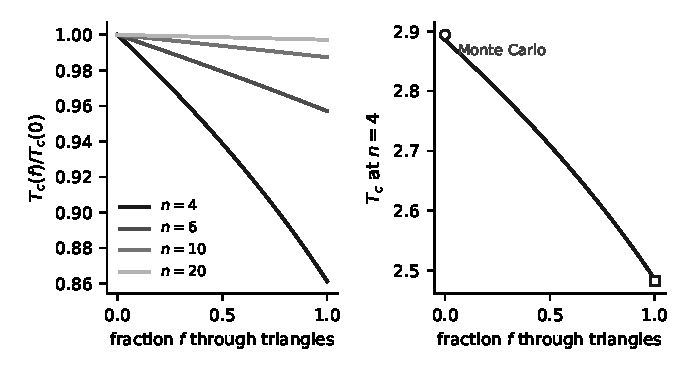
\includegraphics[width=\linewidth]{figs/fig-clustering.pdf}
\caption{\textbf{Clustering lowers $T_{c}$ at fixed degree.} A vertex carries
$fn/2$ triangles and $(1-f)n$ links, so every member of the family has degree
exactly $n$ and the same $p_{d}$; only the clustering coefficient, $f/(n-1)$,
varies. Left: $T_{c}(f)/T_{c}(0)$ from Eq.~\eqref{eq:branch}. The fall is
monotone at every degree and shrinks as the degree grows. Right: the same
family at $n=4$ in absolute units, with the Wolff cluster simulations of
Eq.~\eqref{eq:mc} at $f=0$ and $f=1$ --- open symbols, and they use no cavity
equation. Generated by \code{figs/\allowbreak ising.\allowbreak py}.}
\label{fig:clustering}
\end{figure}

\paragraph{What this does and does not show.} It does not show that a degree
distribution is uninformative. The two ensembles are distinguishable
--- by their clustering coefficient, if by nothing else. What it shows is that
no configuration model on the same degree distribution reproduces the triangle
ensemble's $T_{c}$, and that Eq.~\eqref{eq:uclique} supplies the difference in
closed form. The quantity missing from $\{p_{d},e_{dd'}\}$ is the size of the
shift, and Chapter~\ref{ch:introduction} promised exactly that debt would be
paid here.

\paragraph{The test from outside.} All of the above is one formalism talking to
itself. The check that is not is a direct simulation. Wolff cluster updates on
a $4$-regular random graph and on a network of two triangles per vertex --- the
first row of the table, every vertex at degree exactly $4$ in both --- give
Binder cumulant crossings
\begin{equation}
  T_{c}^{\mathrm{links}}=2.894,
  \qquad
  T_{c}^{\mathrm{tri}}=2.482,
  \label{eq:mc}
\end{equation}
at $n=3000$ and $12000$, against $2.8854$ and $2.4853$ from
Eq.~\eqref{eq:branch}: agreement to $0.30$ and $0.13$ per cent, and a measured shift
of $-14.2$ per cent against a predicted $-13.9$. Both the sign and the size survive
contact with something that has never heard of a cavity equation.

\paragraph{The same null, one order up.} The matched null above carries
Sec.~\ref{sec:magnetisation}'s two observables without change, both of its
members being regular: an $n$-regular graph against a network of $n/2$
triangles per vertex, identical degree distribution either way. Clustering
lowers $T_{c}$ and \emph{raises} both amplitudes
(Table~\ref{tab:amplitudenull}).
\begin{table}[t]
\centering\small
\begin{tabular}{rrrrrrr}
\hline\hline
$n$ & $A_{m}$ links & $A_{m}$ tri. & change & $A_{\chi}$ links & $A_{\chi}$ tri. & change\\
\hline
$4$ & $2.3548$ & $2.8368$ & $+20.5\%$ & $1.4427$ & $1.9883$ & $+37.8\%$\\
$6$ & $2.0926$ & $2.2370$ & $+6.9\%$ & $1.2332$ & $1.3488$ & $+9.4\%$\\
$8$ & $1.9863$ & $2.0572$ & $+3.6\%$ & $1.1587$ & $1.2098$ & $+4.4\%$\\
$10$ & $1.9285$ & $1.9708$ & $+2.2\%$ & $1.1204$ & $1.1493$ & $+2.6\%$\\
$20$ & $1.8241$ & $1.8335$ & $+0.5\%$ & $1.0546$ & $1.0605$ & $+0.6\%$\\
\hline\hline
\end{tabular}
\caption{\textbf{Clustering raises both amplitudes at fixed degree.} The null of Table~\ref{tab:trianglenull}, an $n$-regular graph against a network of $n/2$ triangles per vertex, now read one order up: $A_{m}$ of Eq.~\eqref{eq:magamp} and $A_{\chi}$ of Eq.~\eqref{eq:chiamp}. Both gaps shrink with degree, as the $T_{c}$ gap of Table~\ref{tab:trianglenull} does, and for the same reason. Generated by \code{figs/\allowbreak ising.\allowbreak py}.}
\label{tab:amplitudenull}
\end{table}
The two statements are consistent and it is worth saying why. What the
paragraphs above weighed was multiplicity against transmission at the
transition, and the multiplicity won, so $T_{c}$ fell. The amplitudes are
weighed below the transition, where the lost branch has already been paid for
in the position of $T_{c}$ and what is left is the transmission: at its own
critical temperature the triangle network is the more strongly coupled of the
two per branch, and it leaves the transition faster. So the triangle network
orders at a lower temperature and, once it orders, rises out of the transition
more steeply and responds to a field more strongly. Both gaps die with degree
exactly as the temperature gap does.

\begin{figure}[t]
\centering
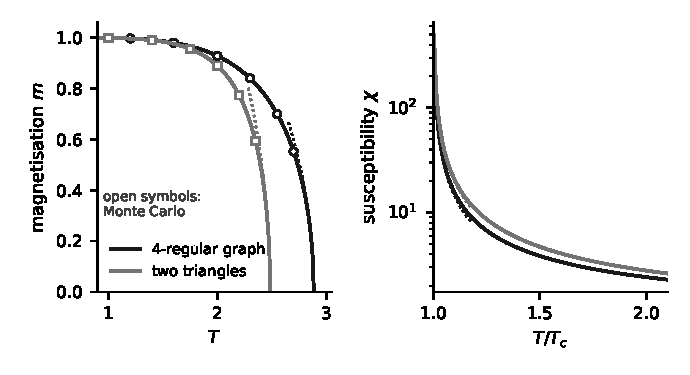
\includegraphics[width=\linewidth]{figs/fig-magnetisation.pdf}
\caption{\textbf{The order parameter and the response.} The matched pair of
this section --- a $4$-regular graph and a network of two triangles
per vertex, degree exactly four in both. Left: the magnetisation from
Eq.~\eqref{eq:magclosure}, with the square-root asymptote
Eq.~\eqref{eq:magamp} dotted and the Wolff simulations of
Eq.~\eqref{eq:mc} as open symbols. Right: the susceptibility from
Eq.~\eqref{eq:chi} against reduced temperature, with the $\gamma=1$ asymptote
Eq.~\eqref{eq:chiamp} dotted; both diverge at their own $T_{c}$, and the
triangle curve lies above because its amplitude is larger. Generated by
\code{figs/\allowbreak ising.\allowbreak py}.}
\label{fig:magnetisation}
\end{figure}

\paragraph{The whole branch, not one point.} Equation~\eqref{eq:magclosure} is
a curve rather than a single temperature, so the Wolff simulations above test
more of the theory than they were run for. The same runs that gave the Binder
crossings give $\ave{m^{2}}^{1/2}$ at every
temperature on the ordered side, and over six temperatures on each structure,
from $T/T_{c}=0.40$ up to $0.95$, the closed form and the simulation agree to
$0.06$ per cent or better at $n=12000$. Nothing in the simulation knows what a
cavity equation is, and the agreement is over the whole branch and not at one
point.

\section{Structured networks}
\label{sec:isingfive}

Chapter~\ref{ch:chygraphs} claimed that one calculation covers the five
structures of Fig.~\ref{fig:mappings}. Sections~\ref{sec:hsfive}
and~\ref{sec:fivecover} pay that out for hitting set and for vertex cover,
where the observable is a threshold in density and the list splits by
cardinality. Here the observable is a temperature and the list barely splits at
all: under the matched null of Sec.~\ref{sec:clustering} the six rows of
Table~\ref{tab:fiveising} take two values, and the sixth lies between them.

That is Eq.~\eqref{eq:tcmulti} doing the work. The condition is one sum over
layers, so a layer list is read off term by term, and two lists with the same
terms give the same temperature however the terms are grouped into structures.

\begin{table}[t]
\centering\small
\begin{adjustbox}{max width=\linewidth}
\begin{tabular}{lccrrr}
\hline\hline
structure & $c$ & $\kappa$ & $T_{c}$ & $T_{c}$ Poisson & AT\\
\hline
A graph & $2$ & $6$ & 4.9326 & 5.9440 & 2.0781\\
A hypergraph & $3$ & $3$ & 4.7209 & 6.8052 & 2.4853\\
A multiplex network & $2,2$ & $3,3$ & 4.9326 & 5.9440 & 2.0781\\
Interacting graphs & $2,2,2$ & $2,2,2$ & 4.9326 & 5.9440 & 2.0781\\
Interacting hypergraphs & $3,3,3$ & $1,1,1$ & 4.7209 & 6.8052 & 2.4853\\
A clustered graph & $2,3$ & $2,2$ & 4.7952 & 6.5400 & 2.3407\\
\hline\hline
\end{tabular}

\end{adjustbox}
\caption{\textbf{The five structures at one degree.} Regular layers, $\kappa$
complexes of each layer per vertex, chosen so that every row sits at degree
exactly six and the six share a degree distribution --- the matched null of
Sec.~\ref{sec:clustering}. $T_{c}$ is Eq.~\eqref{eq:tcmulti}; \emph{AT} is the
same with $u'^{2}$, anticipating Sec.~\ref{sec:atline}. The \emph{Poisson}
column is the identical layer lists with the excess chy-degree left equal to
the mean, which matches the mean degree and nothing else: it reverses the sign,
and is the comparison Sec.~\ref{sec:clustering} warns about. Generated by
\code{figs/\allowbreak ising.\allowbreak py:table\_\allowbreak five\_\allowbreak structures}.}
\label{tab:fiveising}
\end{table}

\paragraph{A graph} is one layer of links. Every $u'$ is $t=\tanh\beta J$ and
there is one term, so Eq.~\eqref{eq:tcmulti} is $\ave{\kbar}\,t=1$, which is
Eq.~\eqref{eq:tcgraph}. For example, the $6$-regular random graph has
$\ave{\kbar}=5$, so $t=1/5$ and $T_{c}=4.9326$. That is the Bethe value, and
the row the others are read against.

\paragraph{A hypergraph} is one complex layer with the cardinality free. Where
that layer carries a single size $c$, which is how every layer in
Chapters~\ref{ch:ising}--\ref{ch:cover} is built, the single term gives
$\ave{\kbar}(c-1)u'(c)=1$ --- the multiplicity $c-1$ against the transmission
$u'(c)$, which is Sec.~\ref{sec:clustering}'s accounting on one line. Where it
carries a distribution of sizes instead, Eq.~\eqref{eq:sbaru}'s size-biased
average takes the place of $(c-1)u'(c)$ and nothing else moves. For
example, a network of triangles at three per vertex, meeting only at vertices so
that the degree is again six, has $\ave{\kbar}=2$, and $2\cdot2\,u'(3)=1$ gives
$T_{c}=4.7209$: the same degree arranged into cliques instead of links, and
colder by $4.3$ per cent. This row is
not a new calculation --- it is the $n=6$ line of Table~\ref{tab:trianglenull},
which is Sec.~\ref{sec:clustering}'s result, arrived at here as one entry in a
list rather than as the chapter's headline.

\paragraph{A multiplex network} is $L$ link layers on the same vertices. Every
layer has $c=2$, so every $u'$ is the same $t$ and Eq.~\eqref{eq:tcmulti} is
\[
  \sum_{l}\frac{\ave{\kappa}_{l}\,t}
                {1-\bigl(\ave{\kbar}_{l}-\ave{\kappa}_{l}\bigr)t}=1,
\]
which is as far as one gets without saying what the degree distribution is. Two
conventions close it. With Poisson layers every
$\ave{\kbar}_{l}=\ave{\kappa}_{l}$, the denominators are $1$, and it is
$Kt=1$ with $K=\sum_{l}\ave{\kappa}_{l}$ the total number of links at a
vertex; with regular layers $\ave{\kbar}_{l}=\ave{\kappa}_{l}-1$, every
denominator is $1+t$, and it is $(K-1)t=1$. Either way only $K$ survives, so a
multiplex is the graph of the same total degree, whatever $L$ is and however the
links are shared out. For example, two $3$-regular link layers give $K=6$, so
$(K-1)t=1$ and $T_{c}=4.9326$, the graph's number exactly. An Ising spin cannot read a layer label, and what
Eq.~\eqref{eq:Hising} sees is the union; that the formalism keeps the layers
apart and still returns one number is the check, not the result.

\paragraph{Interacting graphs and hypergraphs} is $L$ layers whose cardinalities
need not agree --- one layer per interacting structure and a cross layer per
interacting pair, each free to have its own size. In general nothing
simplifies: Eq.~\eqref{eq:tcmulti} stands as it is, one term per layer, and the
layer list is substituted into it. Where the cardinalities do agree, all equal
to $c$, one $u'$ is shared and the previous paragraph goes through with
$(c-1)u'(c)$ in place of $t$:
\[
  \text{Poisson: } K(c-1)\,u'(c)=1,
  \qquad
  \text{regular: } (K-1)(c-1)\,u'(c)=1 ,
\]
so interacting layers of a single cardinality behave as one layer of that
cardinality carrying the total chy-degree. For example, three $2$-regular link
layers give $K=6$ and the graph's $4.9326$; three triangle layers at one
triangle per vertex give $K=3$ and the hypergraph's $4.7209$. So the panel adds
nothing here, and the nothing is worth recording. In Chapters~\ref{ch:hittingset}
and~\ref{ch:cover} the cross layer decides which side of a line the structure
falls on --- whether the hard field is exact there, whether a core-free branch
survives. Equation~\eqref{eq:tcmulti} has no line to fall either side of: a
cross layer contributes its own term to the sum, and the sum is all there is.
The panel that carried the most weight in the two neighbouring chapters carries
the least in this one.

\paragraph{A clustered graph} is a link layer together with one layer per clique
size the graph contains, which is Sec.~\ref{sec:everything}'s mapping. Two
cardinalities or more mean two or more different $u'$ and there is no collapse
to be had: Eq.~\eqref{eq:tcmulti} keeps one term per layer, and at two layers,
expanded, it is Eq.~\eqref{eq:LT}. For example, two links and two triangles per vertex,
degree six for the last time, sits at $4.7952$, between the two. It is Fig.~\ref{fig:clustering}'s family at
$f=2/3$: four of a vertex's six neighbours reached through a triangle, and a
temperature two-thirds of the way from the link value to the triangle one.
Nothing in the row is new either. What the list adds is that the family
Fig.~\ref{fig:clustering} draws is not a special construction but the generic
row --- every structure with more than one cardinality lands inside the
interval, and only the pure ones land on its ends.

\paragraph{The column that misleads.} The Poisson column of
Table~\ref{tab:fiveising} is the warning of Sec.~\ref{sec:clustering}, met again
as a property of the list rather than of one comparison. Leave the excess chy-degree equal to the mean and
every row rises, but the clique rows rise further --- $6.8052$ against $5.9440$
--- and the sign of the whole table reverses. Nothing about the structures has
changed. What changed is that matching the mean degree of a triangle ensemble to
a link ensemble does not match its excess, and Eq.~\eqref{eq:tcmulti} reads the
excess. A reader who built this table without Sec.~\ref{sec:clustering} in front
of them would conclude that clustering raises $T_{c}$ in four of the six rows.

\paragraph{What the list establishes.} Less than the two neighbouring sections
and in a more useful direction. Less, because there is no line for the
structures to fall either side of: Eq.~\eqref{eq:tcmulti} is a single sum, every
structure evaluates it, and the differences between the five are differences of
a few per cent rather than of kind. More useful, because that is the honest
shape of the claim for a thermodynamic observable, and because the one thing the
table does discriminate --- the matched null against the unmatched one --- is not
a property of the chygraph at all. It is a property of the comparison, and it
costs more of the answer here than cardinality does.

\section{The de Almeida--Thouless line}
\label{sec:atline}
\index{de Almeida--Thouless line|textbf}

Section~\ref{sec:replicas} listed three signals that a replica-symmetric answer
has stopped being right, and the first was the stability of the symmetric
solution itself. On a chygraph it costs one character.

Perturb the messages and ask whether the perturbation grows. A perturbation of
\emph{random} sign is transmitted with $u'$ and its effect measured by squaring,
so the relevant condition replaces $\ave{u'}$ by $\ave{u'^{2}}$ everywhere in
Eq.~\eqref{eq:branch} --- and nothing else moves, because the reweighting of
Eq.~\eqref{eq:reweight} is elementwise. On a graph the ferromagnetic line
$\ave{\kbar}t=1$ becomes $\ave{\kbar}t^{2}=1$, both textbook, and on any
chygraph the same substitution serves.

Since $u'\in(0,1)$ gives $u'^{2}<u'$, the spin-glass instability always requires
the stronger coupling: the second row of Sec.~\ref{sec:tc}'s table exceeds the
first at every cardinality, so it is reached only at the lower temperature. For a ferromagnet that is the expected ordering
and the line is not reached, the system ordering first. It becomes the operative
condition when the couplings carry random signs, and it is what
Chapter~\ref{ch:hittingset} will need when its own symmetric solution stops
being trustworthy.

\section{A different interaction inside the complex}
\label{sec:unanimity}
\index{unanimity interaction|textbf}
\index{spinodal}

Nothing in Chapter~\ref{ch:statmech} fixed what is inside a complex.
Equation~\eqref{eq:emitted} sums whatever Hamiltonian is put there and the
chy-degree step never sees it. So a different higher-order interaction is a
substitution rather than a new theory, and this section is the demonstration
that the claim is not empty.

Where Eq.~\eqref{eq:Hising} couples every pair inside a complex, let a hyperedge
instead lower the energy only when \emph{all} its members agree
\citep{son2026}:
\begin{equation}
  \mathcal{H}=-\sum_{e}J_{q}\,\delta_{\{\sigma_{i}\}_{i\in e}}
              -B\sum_{i}\sigma_{i},
  \label{eq:simH}
\end{equation}
with $\delta$ equal to one on the two unanimous states of a hyperedge and zero
on the other $2^{q}-2$. This is the interaction
Chapter~\ref{ch:epidemics} met as a threshold contagion rule --- a group that
acts only when everybody in it acts.

Write the rule as $1+(e^{a}-1)\delta$, $a=\beta J_{q}$, splitting the interior
sum into a free part and one correction. With cavity fields
$h_{1},\dots,h_{q-1}$ on the other members,
\[
  Z(\sigma_{0})=\prod_{j=1}^{q-1}\bigl(2\cosh h_{j}\bigr)
                +(e^{a}-1)\,e^{\sigma_{0}\sum_{j}h_{j}},
\]
the correction surviving only where every $\sigma_{j}=\sigma_{0}$.
Differentiating at $h=0$, the first term contributes nothing and
\[
  u'=\frac{e^{a}-1}{2^{\,q-1}+e^{a}-1}.
\]
Two remarks. This is elementary at \emph{any} cardinality, where the all-pairs
clique of Sec.~\ref{sec:transmits} needs an enumeration --- so a harder-looking
interaction can be easier inside. And at $q=2$ it is $\tanh(a/2)$: a unanimous
pair is an ordinary bond of half the coupling, as
$\delta_{\sigma_{0}\sigma_{1}}=(1+\sigma_{0}\sigma_{1})/2$ requires.

One trap. The equation above is the derivative with respect to \emph{one} other
member's field, the same convention as Eq.~\eqref{eq:uprime}, so the
multiplicity $q-1$ is supplied by Eq.~\eqref{eq:branch} and not here.
Differentiating instead with respect to a field common to all $q-1$ others
multiplies it by $q-1$; using \emph{that} in Eq.~\eqref{eq:branch} counts the
multiplicity twice. \code{Chygraph.\allowbreak simplicial} returns both: \code{emitted} is the
interior and \code{spinodal} the condition built on it, in the module
\code{simplicial}.

\paragraph{The infinite-connectivity limit.} Take one layer of cardinality $q$
at fixed chy-degree $k$ and impose \citeauthor{son2026}'s normalisation
$J_{q}=q/k$. Expanding the spinodal condition $(k-1)(q-1)u'=1$ in $1/k$,
\begin{equation}
  T^{*}\longrightarrow\frac{q(q-1)}{2^{\,q-1}}
  \qquad(k\to\infty),
  \label{eq:BW}
\end{equation}
which is their mean-field result, approached with residual
\begin{equation}
  T-T^{*}=-\frac{C_{q}}{k}+O(k^{-2}),
  \qquad
  C_{q}=\frac{q\bigl(2q-2^{\,q-1}\bigr)}{2^{\,q}}.
  \label{eq:Cq}
\end{equation}
Equation~\eqref{eq:BW} is non-monotonic in cardinality, peaking at $q=3$ and
$q=4$ together (Fig.~\ref{fig:unanimity}), and at finite chy-degree the
degeneracy is lifted. The coefficient $C_{q}$ vanishes when
$2q=2^{\,q-1}$, that is at $q=4$ and nowhere else. The leading
finite-connectivity correction is absent at exactly the cardinality that is
tricritical in the mean-field theory, so $T^{*}$ is approached there as $1/k^{2}$
rather than $1/k$ --- $-2.2\times10^{-5}$ at $k=200$ against
$-3.8\times10^{-3}$ at $q=3$.

\begin{figure}[t]
\centering
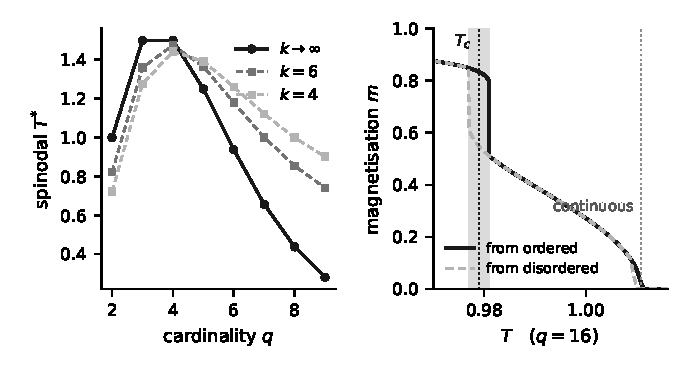
\includegraphics[width=\linewidth]{figs/fig-unanimity.pdf}
\caption{\textbf{A different interior, and a warning.} Left: the spinodal
against cardinality for the unanimity rule under the normalisation
$J_{q}=q/k$, at chy-degrees $4$ and $6$ and in the limit
Eq.~\eqref{eq:BW}. It is non-monotonic, and finite connectivity shifts where it
peaks. Right: the double transition at $q=16$ with
$(J_{q},J_{2},k_{q},k_{2})=(0.3,0.7,4,4)$, continued from an ordered and from a
disordered start. The continuous transition sits at $T=1.0108$; inside the
shaded coexistence window the two branches differ, and the free energies cross
at $T_{c}=0.9790$, where $m$ jumps by $0.286$. Generated by
\code{figs/\allowbreak ising.\allowbreak py}.}
\label{fig:unanimity}
\end{figure}

\paragraph{Where the branching condition stops being the transition.} For this
model, most of the interesting range is discontinuous, and there
Eq.~\eqref{eq:det} locates a spinodal rather than a transition. This is the
fourth time the book has arrived here --- Sec.~\ref{sec:breakdown} for
interdependent networks, Sec.~\ref{sec:groupcontagion} for threshold contagion,
Sec.~\ref{sec:transmission} for the Potts model above $q=2$ --- and it is the
first time the tool built in Sec.~\ref{sec:freeenergy} is actually used.

The right-hand panel of Fig.~\ref{fig:unanimity} is the calculation done
properly. At $q=16$ with $(J_{q},J_{2},k_{q},k_{2})=(0.3,0.7,4,4)$ there are two
transitions. The upper one is continuous, at $T=1.0108$, and it is essentially
the pairwise value: $u'$ is $O(2^{-q})$ at $q=16$, so the higher-order layer
contributes nothing to the linear instability. The lower one is first order. Iterating from a magnetised start and from a near-zero one, the two
branches differ on $0.9770<T<0.9810$; comparing Eq.~\eqref{eq:bethe} between
them inside that window, they cross at
\begin{equation}
  T_{c}=0.9790,\qquad \Delta m=0.286,
\end{equation}
with $m$ jumping from $0.548$ to $0.834$, and $T^{*}<T_{c}<T^{**}$ as it must.

\paragraph{A test that has to be done carefully.} Whether the transition at a
given $(q,k)$ is continuous or discontinuous is the sort of question that
invites a quick answer and is easy to get wrong. Iterating from an ordered start just
above the spinodal and finding a non-zero magnetisation looks like evidence of
coexistence --- but just above a \emph{continuous} transition the ordered branch
decays so slowly that a finite iteration budget reports exactly the same thing.
Critical slowing down mimics a first-order window.

Done properly --- a converged branch, a coexistence window of non-negligible
width, and a free-energy crossing strictly inside it --- the boundary sits
between $q=5$ and $q=6$ at chy-degree $3$, and between $q=4$ and $q=5$ from
chy-degree $4$ upward. Low connectivity delays the discontinuity by one in
cardinality and then stops mattering. At chy-degree $4$ and $q=5$, for instance,
the window is $1.1138<T<1.1308$ and the free energies cross at $T_{c}=1.1262$:
narrow, but real. At $q=4$ the apparent window is thirty times narrower and
holds no crossing at all, at chy-degree $4$, $6$, $10$ or $40$. That is the
difference between an artefact and a transition, and it is only visible if one
looks for the crossing.

\section{Checks}
\label{sec:ising-checks}

\checkhead{Known results}
On a graph the condition $\ave{\kbar}\tanh\beta J=1$ is the textbook Bethe
temperature, and Sec.~\ref{sec:tc}'s $u'$ is Chapter~\ref{ch:potts}'s
$\tau_{c}(2,v)$, checked in Sec.~\ref{sec:statmech-checks}.
With the Ising interior substituted, Eq.~\eqref{eq:chi} returns the
Bethe-lattice susceptibility Eq.~\eqref{eq:chibethe} on a regular graph and
$1/(1-\ave{k}t)$ on a Poisson one, to eleven digits at three couplings each;
both are textbook. Equation~\eqref{eq:magamp} reduces to
Eq.~\eqref{eq:magampgraph}, checked to $10^{-8}$ at $k=3,4,6,10$, and tends to
the Curie--Weiss value $\sqrt3$ as the degree grows --- $1.7338$ at $k=1000$
against $1.7321$. Equation~\eqref{eq:BW}'s infinite-connectivity limit
$T^{*}\to q(q-1)/2^{q-1}$ is \citeauthor{son2026}'s mean-field value, recovered
here by expanding the spinodal condition in $1/k$.

\checkhead{New results}
The rest of the chapter has no published counterpart.
Equation~\eqref{eq:uclique} is checked against the numerical enumeration behind
Eq.~\eqref{eq:emitted} at four couplings for $c=2,3,4$, and the closed form for
the unanimity rule likewise. Equation~\eqref{eq:tcmulti} reduces to
Eq.~\eqref{eq:LT} on expanding its two-layer case, and is checked against the
Perron root of Eq.~\eqref{eq:branch} to $10^{-9}$ on each of
Table~\ref{tab:fiveising}'s six layer lists. That table's graph and hypergraph
rows are the $n=6$ line of Table~\ref{tab:trianglenull} reached by the other
route; its three cardinality-two rows are checked to agree, its two pure-clique
rows likewise, and the mixed row to lie between them.
The two amplitudes are Sec.~\ref{sec:response}'s and are checked there; what
this chapter adds to them is the interior. Equation~\eqref{eq:a1a3}'s cumulants
are checked twice for the all-pairs clique: $a_{1}$ against the transmission
$(c-1)u'$ the threshold already uses, to twelve digits at $c=2,\dots,5$, and
$a_{3}$ against Eq.~\eqref{eq:a3edge} at $c=2$ and against finite differences of
the enumeration itself above it. And Eq.~\eqref{eq:magclosure} reproduces the
whole ordered branch, not one point: against the Wolff simulations at $n=12000$
it agrees to $0.06$ per cent or better at six temperatures on each of the two
structures of Sec.~\ref{sec:clustering}, from $T/T_{c}=0.40$ to $0.95$. That is
the one test of the order parameter from outside the formalism. Equation~\eqref{eq:Cq} is checked against the
spinodal computed from Eq.~\eqref{eq:det} at $k=200$ for $q=2,\dots,8$,
including the case $q=4$ where the prediction is that the correction
\emph{vanishes} and the residual duly falls to $2\times10^{-5}$. Carrying the
message as a distribution and iterating a population of samples --- the up step
a Poisson-compound convolution, the down step Eq.~\eqref{eq:emitted} evaluated
numerically --- gives $\beta J_{c}=0.164628$ against the closed-form $0.168236$
for a graph at six neighbours, and $0.144343$ against $0.146947$ for the
corresponding triangle network; independently, the gap between the ordered and
paramagnetic branches of Eq.~\eqref{eq:bethe} is zero to machine precision below
the transition and lifts off above it, in the same place. And
Eq.~\eqref{eq:mc}: the Wolff simulations use no cavity equation and confirm both
the sign and the size of the clustering effect. That is the only number in the
chapter that could have come out differently.

\checkhead{Partial results}
Equation~\eqref{eq:magclosure} carries Sec.~\ref{sec:response}'s restriction
into this chapter: it covers the two ends of Fig.~\ref{fig:clustering}'s family
and none of its interior, whose members give a vertex a fractional number of
triangles. Checking the closure against a population on a \emph{regular}
chygraph tests the excess bookkeeping of both routes and not the physics of
either, because a regular chygraph collapses the population onto one value; the
Monte Carlo above is the check that is not of that kind.
The population dynamics is low by $2.1$ and $1.8$ per cent, for a definite reason ---
a finite sweep budget calls a slowly decaying magnetisation ordered, which is
the same effect as the trap in Sec.~\ref{sec:unanimity} --- so it confirms the
closed forms rather than competing with them. Nothing here is evidence that the
treelike assumption holds on a real network: both simulated ensembles were built
so that their triangles share at most one atom, which is the condition the
theory needs and which Chapter~\ref{ch:data} showed real networks violate.
Chapter~\ref{ch:overlap} measures what that violation costs.


% sources
% - the retired manuscript, Sec. IV and supplement Secs. III-IV
% - ../examples/clustering_lowers_tc.py

\chapter{Hitting set}
\label{ch:hittingset}
\index{hitting set problem}

Chapters~\ref{ch:potts}--\ref{ch:ising} carried one number per inclusion all the
way from $q=1$ to $q=\infty$. This chapter is where that stops.
The failure it identifies, and the repair, are new here; the closed forms it
reproduces at cardinality two are those of \citet{weigt2000} and
\citet{mezard2007}, and are attributed at each use.

The problem is a hard-core one: minimise a set subject to a constraint that some
configurations are simply forbidden. Nothing in Chapter~\ref{ch:statmech}
objects --- Eq.~\eqref{eq:emitted} sums whatever is inside a complex, and an
infinite energy is a legitimate thing to put there. What changes is that the
standard way of taking the zero-temperature limit, which is exact on a graph and
has been used on graphs for twenty-five years, is \emph{wrong} on a hypergraph.
Section~\ref{sec:hardfail} gives a counterexample small enough to check by hand,
and Sec.~\ref{sec:soft} gives the repair.

The failure is this chapter's version of something the book keeps returning to.
It is not that the cavity method fails on higher-order structures. It is that a
simplification which is invisible on a graph, because it costs nothing there,
becomes the whole error once complexes hold more than two nodes.

\section{Covering a family of sets}
\label{sec:hittingsetdef}

A \emph{hitting set} meets every hyperedge: a set of nodes such that no
hyperedge is left entirely outside it. Minimising it generalises vertex cover
from graphs to hypergraphs \citep{mezard2007}. Put $x_{i}=1$ when node $i$ is in
the set and $x_{i}=0$ when it is not, and write
\begin{equation}
  \mathcal{H}=\mu\sum_{i}x_{i}
  \qquad\text{subject to}\qquad
  \prod_{e}\Bigl[1-\prod_{i\in e}(1-x_{i})\Bigr]=1,
  \label{eq:Hhs}
\end{equation}
the constraint forbidding a hyperedge none of whose members is taken, and the
chemical potential $\mu$ penalising every member, so that minimum hitting sets
are the ground states reached as $\mu\to\infty$.

At cardinality two this is minimum vertex cover, Sec.~\ref{sec:cover-intro}, and
Chapter~\ref{ch:cover} is what happens when the constraint is tightened instead
of the cardinality raised. The two problems sit at opposite ends of one family
and differ in one line of the interior sum. The failure this chapter is about is
invisible at cardinality two, which is where the literature works.

It is often convenient to work with the complement $y_{i}=1-x_{i}$, which is a
\emph{packing} --- no hyperedge lies wholly inside it --- since the hard-field
limit is naturally written that way, the cover being one minus the packing
density.

\section{Hard fields}
\label{sec:hard}
\index{hard field|textbf}
\index{warning propagation|textbf}

The standard treatment rescales the cavity fields, which diverge as
$\mu\to\infty$: put $h=\mu z$ and keep only the integer $z$. The up step of
Eq.~\eqref{eq:up} becomes a count,
\begin{equation}
  z_{i}=1-\#\bigl\{\,b\ni i:\ z_{j\to b}=1\ \ \forall\,j\in b\setminus i\,\bigr\},
  \label{eq:zhs}
\end{equation}
which is \emph{warning propagation}: a complex sends a warning when every one of
its other members is free to stay out, and a node counts its warnings.

Two steps take that to an ensemble. Let $\sigma_{l}$ be the probability that a
node reached along an inclusion into a layer-$l$ complex has $z=1$, that is, is
free to stay out. A layer-$l$ complex entered at $i$ warns $i$ exactly when
every one of its other $c_{l}-1$ members is free, and on a treelike chygraph
those members are independent given what reaches them, so
$\tau_{l}=\sigma_{l}^{\,c_{l}-1}$. And $i$ is free precisely when \emph{none} of
its other complexes warns it; each fails to warn with probability $1-\tau$, how
many others there are is the excess chy-degree of Sec.~\ref{sec:ensembles}, and
averaging a product over that count is evaluating its generating function. So
\begin{equation}
  \sigma_{m}=\bar\Phi^{(m)}(1-\tau),
  \qquad
  \tau_{l}=\sigma_{l}^{\,c_{l}-1}.
  \label{eq:hs}
\end{equation}
Section~\ref{sec:twoconstraints} does the same two steps for vertex cover and
gets the complement in the other place, for the reason given there: a hyperedge
forces when \emph{all} of its other members are free and a clique forces when
\emph{any} of them is. \code{hittingset.HittingSet.F} is the map and
\code{hittingset.HittingSet.solve} its fixed point.

\paragraph{The map runs backwards.} Equation~\eqref{eq:hs} is
order-\emph{reversing}: raising any message lowers every message. This is not a
technicality. Plain iteration oscillates, and past the point where the map loses
stability it never settles --- which is how the instability was originally
detected \citep{vazquez2003vw}, by noticing that the program stopped converging.
It is also the diagnostic Sec.~\ref{sec:fixedpoint} said would be needed, and
the reason it insisted on reading the \emph{signs of the entries} rather than
the sign of the leading eigenvalue.

It need not be left to chance. For $F$ continuous and order-reversing on
$[0,1]^{L}$ --- both hold here, since $\bar\Phi$ is a power series with
non-negative coefficients and $\sigma\mapsto1-\sigma^{c-1}$ is decreasing ---
the composition $F\circ F$ is order-\emph{preserving}. Iterating $F\circ F$ from
$0$ and from $1$ therefore returns its least and greatest fixed points $a\le b$
with $F(a)=b$. If $a=b$ there is a single stable fixed point; if $a<b$ there is
a period-two orbit with the fixed point of $F$ strictly between them, unstable.
The bracket finds the solution and diagnoses it in one pass, which is a better
bargain than watching an iteration fail to converge.

\paragraph{Where it loses stability.} At fixed cardinality $c$ with Poisson
chy-degree, $\bar\Phi(x)=e^{\ave{k}(x-1)}$ and Eq.~\eqref{eq:hs} closes on one
scalar.

With one layer and Poisson chy-degree the map is
$\sigma=e^{-\ave{k}\sigma^{c-1}}$. Differentiating and using the fixed-point
relation,
\[
  |F'(\sigma)|=\ave{k}(c-1)\sigma^{c-2}e^{-\ave{k}\sigma^{c-1}}
             =\ave{k}(c-1)\sigma^{c-1}.
\]
Put $y=\ave{k}\sigma^{c-1}$. The fixed point reads $\sigma=e^{-y}$ and
$y=\ave{k}e^{-(c-1)y}$, while the instability $|F'|=1$ is $(c-1)y=1$.
Eliminating $y=1/(c-1)$ from the second,
\[
  \ave{k}=y\,e^{(c-1)y}=\frac{e}{c-1},
  \qquad\text{that is}\qquad
  \ave{k}\,(c-1)=e.
\] \code{hittingset.\allowbreak rsb\_\allowbreak point} solves it, and returns $e$ at $c=2$ to ten digits.

So
\begin{equation}
  \ave{k}\,(c-1)=e,
  \label{eq:kc}
\end{equation}
verified to eleven digits for $c=2,\dots,20$. Read in \emph{neighbours} per
node, cardinality does not move the point at all: a hyperedge of size six
supplies five neighbours and costs a fifth of the chy-degree, and the two cancel
exactly. At $c=2$ this returns $\ave{k}=e$, the Bauer--Golinelli value
\citep{bauer2001}, which Chapter~\ref{ch:cover} will show is three quantities
with one name.

\paragraph{What Eq.~\eqref{eq:kc} is a statement about.} It locates the loss of
stability of the \emph{hard-field} map --- which is to say, where
leaf-removal-style certification stops. At $c=2$ that coincides with the
accepted replica-symmetry-breaking point, which is why $e$ comes out. Above
$c=2$ it does not, and the next section is why.

\section{Where the hard-field limit breaks}
\label{sec:hardfail}
\index{hard field}

Equation~\eqref{eq:zhs} discards an $O(1)$ contribution: it keeps the part of
$h$ proportional to $\mu$ and throws away the remainder. On a graph the discard
is harmless. On a hypergraph it is the answer.

The cleanest demonstration needs no computer. Take disjoint $3$-hyperedges, one
per vertex --- so every vertex belongs to exactly one hyperedge and no two
hyperedges touch (Fig.~\ref{fig:counterexample}). There is no interaction
between complexes at all. Replica symmetry is trivially valid, there is nothing
for it to break. One of every three vertices must be taken, so the minimum
hitting set has density exactly $1/3$.

The hard-field calculation returns $1/2$.

\begin{figure}[t]
\centering
\begin{adjustbox}{max width=0.95\linewidth}
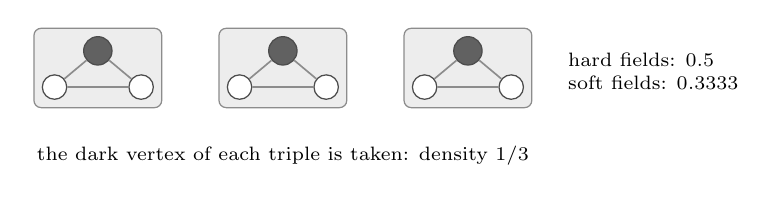
\begin{tikzpicture}
% Three disjoint 3-hyperedges. Nothing couples them, so replica symmetry is
% trivially valid and the answer is exactly 1/3 -- which is what makes this a
% counterexample rather than a hard case.
\foreach \s in {0,1,2}{
  \begin{scope}[xshift=\s*2.35cm]
    \node[nd] (a\s) at (-0.55,0) {};
    \node[hub] (b\s) at (0.0,0.46) {};
    \node[nd] (c\s) at (0.55,0) {};
    \draw[lnk] (a\s)--(b\s)--(c\s)--(a\s);
    \begin{scope}[on background layer]
      \node[cx,fit=(a\s)(b\s)(c\s)] {};
    \end{scope}
  \end{scope}
}
\node[lb,anchor=north,align=center] at (2.35,-0.62)
  {the dark vertex of each triple is taken: density $1/3$};
\node[lb,anchor=west,align=left] at (5.85,0.20)
  {hard fields: $0.5$\\ soft fields: $0.3333$};
\end{tikzpicture}
\end{adjustbox}
\caption{\textbf{A counterexample that fits on one line.} Disjoint
$3$-hyperedges, one per vertex. No complex touches another, so the cavity
equations are exact and replica symmetry cannot break. One vertex per hyperedge
must be taken and the density is exactly $1/3$. The hard-field limit,
Eq.~\eqref{eq:zhs}, returns $1/2$ --- and its bracket is the whole interval
$(0,1)$, so it cannot even report that it is in trouble. Keeping the $O(1)$
fields, Eq.~\eqref{eq:soft}, returns $1/3$.}
\label{fig:counterexample}
\end{figure}

The mechanism is precise. Inside such a hyperedge every vertex sits at $z=0$: the
integer message cannot distinguish the taken vertex from the two left out,
because the distinction is carried by the $O(1)$ part that was scaled away. A
vertex at $z=0$ is degenerate, and the standard rule counts it as half covered
--- which is right when the degeneracy is two-fold, as it is on a graph, and
wrong when it is three-fold. The bracket of Sec.~\ref{sec:hard} returns $(0,1)$
here, so the hard-field scheme cannot even report that it is in difficulty.

The second failure follows from the first. Equation~\eqref{eq:kc} is a property
of the hard-field map and not of the full replica-symmetric solution, and the
two coincide only at cardinality two. On random regular hypergraphs the
hard-field criterion reports broken symmetry across almost the whole grid where
\citet{mezard2007} find a genuine replica-symmetric region --- though it
does reproduce their result that cardinality two breaks at every degree.

\section{Keeping the fields}
\label{sec:soft}
\index{soft field|textbf}
\index{population dynamics}

Both failures are repaired by not scaling the fields at all.

Work directly with Eq.~\eqref{eq:Hhs}: $x_{i}=1$ for a vertex in the set, weight
$e^{-\mu\sum_{i}x_{i}}$, no change of variable. Belief propagation on the
chygraph then reads
\begin{align}
  v_{a\to i}&=-\ln\Bigl[1-\prod_{j\in a\setminus i}
                \bigl(1+e^{h_{j\to a}}\bigr)^{-1}\Bigr],\nonumber\\
  h_{i\to a}&=-\mu+\sum_{b\ni i,\ b\ne a}v_{b\to i},
  \label{eq:soft}
\end{align}
with the density read off the full field,
$\rho=\bigl[1+e^{\,\mu-\sum_{b\ni i}v_{b\to i}}\bigr]^{-1}$.

These are Chapter~\ref{ch:statmech}'s two steps and nothing else. The chy-degree
step is the convolution of Sec.~\ref{sec:upstep}; the complex step is the sum
over the interior of Sec.~\ref{sec:downstep}, here over the single forbidden
configuration in which no member is taken. What has changed against
Sec.~\ref{sec:hard} is only that nothing is divided by $\mu$, so the $O(1)$
parts survive and $\rho$ emerges as a genuine $O(1)$ number rather than a count
of integers.

For a regular hypergraph --- $L$ complexes per node, each of cardinality $K$ ---
symmetry makes every message equal and Eq.~\eqref{eq:soft} closes on a pair:
\[
  h=-\mu+(L-1)v,
  \qquad
  v=-\ln\Bigl[1-\bigl(1+e^{h}\bigr)^{-(K-1)}\Bigr].
\]
As $\mu\to\infty$, $h\to-\infty$ and
$(1+e^{h})^{-(K-1)}=1-(K-1)e^{h}+O(e^{2h})$, so the complex step becomes
$v=-\ln(K-1)-h$. Substituting, $Lh=-\mu-(L-1)\ln(K-1)$, that is
\begin{equation}
  h_{\mathrm{RS}}=-\frac{\mu}{L}-\frac{L-1}{L}\ln(K-1).
  \label{eq:hRS}
\end{equation}
The cavity field carries a \emph{fraction} $1/L$ of $\mu$. An ansatz restricted to integer multiples of $\mu$ cannot represent it,
and that --- not any subtlety about correlations --- is why
Sec.~\ref{sec:hardfail} fails.

The full field is finite, $H=h+v=-\ln(K-1)$, so
\[
  \rho=\frac{1}{1+e^{-H}}=\frac1K,
\]
independent of $\mu$ \emph{and} of $L$: one member of every complex is taken and
none is wasted, so the counting bound is saturated exactly. \code{softfield.\allowbreak regular\_\allowbreak field} is the closed form,
and the population dynamics it is checked against is
\code{Chygraph.\allowbreak hitting\_\allowbreak set\_\allowbreak bp}, over
\code{softfield.\allowbreak HittingSetBP}.

Equation~\eqref{eq:hRS} and $\rho=1/K$ are the closed forms of
\citet{mezard2007}, and population dynamics reproduces both --- the field
to five decimals, the density to four. The repair is complete on the
counterexample too: disjoint $3$-hyperedges return $0.3333$.
Figure~\ref{fig:hitting} runs the comparison across ensembles.

\begin{figure}[t]
\centering
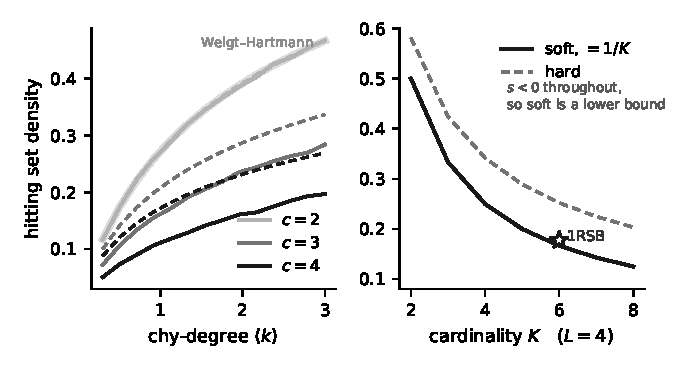
\includegraphics[width=\linewidth]{figs/fig-hitting.pdf}
\caption{\textbf{The repair.} Minimum hitting-set density from the hard-field
limit, Eq.~\eqref{eq:hs} with the half rule (dashed), and from
Eq.~\eqref{eq:soft}, which keeps the $O(1)$ fields (solid). Left: Poisson
layers of one cardinality, with the Weigt--Hartmann closed form drawn thick
behind the $c=2$ curves, which the two treatments share exactly. They separate
above cardinality two and the gap grows with $c$. Right: regular hypergraphs at
$L=4$. The soft field returns $\rho=1/K$; the hard field does not; and at $K=6$
the two bracket the one-step replica-symmetry-breaking value of
\citet{mezard2007} (star), $0.1667<0.178<0.2522$. Generated by
\code{figs/\allowbreak hittingset.\allowbreak py}.}
\label{fig:hitting}
\end{figure}

At cardinality two hard and soft \emph{must} agree, and do: both return the
Weigt--Hartmann cover size $1-(2W+W^{2})/(2\ave{k})$ with
$W=\mathcal{W}(\ave{k})$, the hard field to six digits and the soft field to
within its sampling scatter of a few parts in a thousand. Above cardinality two
the correction grows with the weight the ensemble puts on complexes of three or
more members: for a Poisson layer of $c=4$ alone at $\ave{k}=1$ the hard field
overstates the density by about $55$ per cent, $0.172$ against $0.111$, and for
a mixture of $c=2$ and $c=6$ at chy-degrees $1.5$ and $0.5$ by under one per
cent. That last number is the reassuring one: it says the twenty-five years
of graph results were never in danger.

\section{What the chygraph structure adds}
\label{sec:hsstructures}

Equation~\eqref{eq:soft} carries an arbitrary chy-degree distribution, mixed
cardinalities and correlated layers, none of which a regular ansatz reaches.
Two effects, pointing in opposite directions.

\emph{Spread in cardinality postpones the difficulty.} Hold fixed the mean
number of neighbours a complex supplies, $\nu=\sum_{l}\ave{k_{l}}(c_{l}-1)
/\sum_{l}\ave{k_{l}}$, at $2$, and report $\ave{k}\nu$, the neighbours per node
at which Eq.~\eqref{eq:kc}'s instability arrives. It runs from $2.72$ for
uniform $c=3$, to $4.84$ for an equal mixture of $c=2$ and $c=4$, to $6.83$ for
a three-to-one mixture of $c=2$ and $c=6$. Heterogeneity keeps certification
working longer, which is the direction degree heterogeneity acts in as well
\citep{vazquez2003vw}.

\emph{Correlation across cardinalities brings it forward.} Anti-correlate a
node's participation in small and in large hyperedges, holding the marginals
fixed, and the point moves monotonically down from $6.83$ to $2.64$. This axis has no counterpart
in an ensemble with one edge type, and it is the sort of thing
Chapter~\ref{ch:data} recommended measuring rather than assuming away.

\paragraph{A confound.} The obvious positive-correlation
construction --- half the nodes at double the chy-degree, half at zero ---
returns a point at exactly half the uncorrelated value, and that is not
correlation but \emph{dilution}: the zero class is a set of isolated vertices.
Matched constructions keep both classes populated, and $\Phi(0,\dots,0)$, the
fraction of vertices in no hyperedge at all, should be reported alongside any
such comparison. On the positive branch it rises from $0.033$ to $0.47$ as the
correlation is pushed to its extreme, so only its small-spread end is a clean
measurement. The negative branch is cleaner but not innocent. Neither class ever
empties there, since anti-correlation moves chy-degree between the layers rather
than out of both at once; but the ensemble is sparser at its own threshold, and
$\Phi(0,\dots,0)$ still runs $0.033$, $0.047$, $0.198$, $0.321$ across the four
spreads. The direction is settled at the second of those, where dilution is
negligible and the point has already moved from $6.83$ to $6.50$. The size of
the full excursion to $2.64$ is not separable from the dilution that comes with
it, and is not quoted as though it were.

\section{When replica symmetry fails}
\label{sec:hsrsb}
\index{replica symmetry breaking}

Section~\ref{sec:replicas} listed three signals. This chapter can now supply the
second, and it is the one that carries a number.

The Bethe free energy of Sec.~\ref{sec:freeenergy} applies unchanged, with
$Z_{i}=1+e^{H_{i}}$ and $Z_{a}=\prod_{i\in a}(1+e^{h_{i\to a}})-1$ --- the
complex term being the sum over its interior with the one forbidden
configuration removed --- so that
\begin{equation}
  s=\sum_{l}n_{l}\ave{\ln Z_{a}}+\ave{(1-k)\ln Z_{i}}+\mu\rho.
  \label{eq:sgen}
\end{equation}
For a regular hypergraph this reduces to
\begin{equation}
  s=\frac{1}{K}\bigl[a\ln(K-1)-(a-1)\ln K\bigr],
  \qquad
  a=(L-1)(K-1),
  \label{eq:entropy}
\end{equation}
which is \citeauthor{mezard2007}'s expression, reproduced by
Eq.~\eqref{eq:sgen} to nine digits. Since $s$ is the logarithm of a number of
ground states, a negative value counts fewer than one configuration, which is
impossible: where $s<0$ the replica-symmetric answer is wrong and is an
\emph{underestimate}. At $L=4$, $K=6$ the entropy is $-0.157$, and indeed the
replica-symmetric $1/6$ sits below the one-step $0.178$ while the hard-field
$0.252$ sits above it and further away.

Three qualifications, and all three matter in practice.

\emph{It is sufficient but not necessary.} A negative $s$ proves the answer
wrong; a positive $s$ does not prove it right, since a solution can be unstable
while its entropy is still positive. Vertex cover on Poisson graphs is the
standing example: replica symmetry breaks at $\ave{k}=e$, and yet
Eq.~\eqref{eq:sgen} returns $s=+0.088(26)$ at $\ave{k}=1$ and a value still
positive at $3$. The entropy has to be paired with a stability criterion, not
used alone.

\emph{It is not numerically cheap.} In Eq.~\eqref{eq:sgen} the terms
$\sum_{l}n_{l}\ave{\ln Z_{a}}$ and $\mu\rho$ are each $O(\mu)$ while $s$ is
$O(1)$, so a heterogeneous ensemble needs both to a relative precision of order
$s/\mu$ and only time-averaging the estimator brings that within reach. The
regular case is exact because symmetry removes the sampling entirely --- the two
$O(\mu)$ pieces cancel algebraically rather than statistically.

\emph{The third signal still shows up.} At $L=6$, $K=12$ the closed-form entropy
is $-0.192$ and the iteration simply does not settle; the estimator returns a
small positive number that means nothing. That is Sec.~\ref{sec:replicas}'s
third signal --- the equations stop converging --- and it is the same failure
the negative entropy reports, arriving by a different route.

What one-step replica symmetry breaking would change here, this book does not
compute. Sections~\ref{sec:colouring-sp} and~\ref{sec:sat-sp} do the one-step
calculation for two problems whose messages are warnings, where a survey is a
distribution over a finite alphabet; a hitting-set field is a real number and
the survey is a distribution over distributions, which is a heavier object and
is not attempted. What this chapter can say is where the replica-symmetric
answer stops being trustworthy, and on which side of the truth it then falls.

\section{Checks}
\label{sec:hs-checks}

\checkhead{Known results}
At cardinality two both treatments return the Weigt--Hartmann cover size, the
hard field to six digits, and Eq.~\eqref{eq:kc} returns $e$ there, which is
Bauer--Golinelli. Equations~\eqref{eq:hRS} and~\eqref{eq:entropy} reproduce
\citeauthor{mezard2007}'s closed forms, the first to five decimals by population
dynamics and the second to nine digits by Eq.~\eqref{eq:sgen}.

\checkhead{New results}
Everything above cardinality two is new here: the failure of the hard-field
limit, the repair, and Eq.~\eqref{eq:kc} away from $c=2$, which is verified to
eleven digits for $c=2,\dots,20$. The failure is checked against arithmetic
rather than against the literature. Section~\ref{sec:hardfail}'s counterexample
is not a numerical check but a proof: the answer is $1/3$ by counting, the soft
field returns $0.3333$, and the hard field returns $0.5$. Nothing about it
depends on an implementation being right.

\checkhead{Partial results}
Soft-field densities on Poisson ensembles come from a population of finite size
and carry a scatter of a few parts in a thousand that does not shrink cleanly
with the population; they are quoted to three decimals with the spread across
seeds beside them, and the regular cases carry no such scatter. The entropy of
Eq.~\eqref{eq:sgen} is sufficient and not necessary: a negative value proves the
replica-symmetric answer wrong, a positive one proves nothing, and vertex cover
on Poisson graphs is the standing example. What replica symmetry breaking would
change is not computed --- a hitting-set field is a real number, so the survey is
a distribution over distributions, and Sec.~\ref{sec:hsrsb} states the cost and
stops there.


% sources
% - the retired manuscript, Sec. V and supplement Sec. V
% - ../examples/softfield_vs_hardfield.py, ../examples/hitting_set_rsb.py

\chapter{Vertex covering}
\label{ch:cover}
\index{vertex cover}

A \emph{vertex cover} is a set of nodes touching every link, and the problem is
to find the smallest one. Section~\ref{sec:cover-intro} put it as a model ---
$x_{i}\in\{0,1\}$ on every node, the energy $\sum_{i}x_{i}$ to be minimised, and
a hard constraint $x_{i}+x_{j}\ge1$ on every link --- and it is NP-hard
\citep{karp1972}. It is also Chapter~\ref{ch:hittingset}'s hitting set at
cardinality two, which is why the two chapters are adjacent.

This chapter solves it on a chygraph. The constraint is then read over every
pair inside every complex, so a complex is a clique that has to be covered, and
what the chapter asks is what that changes: how small a cover can be when the
links arrive in triangles and cliques rather than one at a time, and how much
harder it is to find one.

Three methods answer that, in the order Chapter~\ref{ch:statmech} sets and
Chapters~\ref{ch:ising} and~\ref{ch:hittingset} follow.
Section~\ref{sec:twoconstraints} writes the interior down and reads off what a
complex transmits, which is the cavity recursion.
Section~\ref{sec:leafremoval} is leaf removal,
Sec.~\ref{sec:leafremoval-intro}'s combinatorial rule, which that recursion
turns out to describe exactly. Section~\ref{sec:coreobstruction} treats what
the rule gets stuck on --- the core --- by the LCZP map of \citet{liu2012}, a
cavity calculation carrying three states rather than one, since a node may be
settled in either of two ways or in neither.
Section~\ref{sec:fivecover} then runs the three of them over the five
structures of Fig.~\ref{fig:mappings}, one paragraph each, which is where
Chapter~\ref{ch:chygraphs}'s claim about substitution is paid out or is not.
Sections~\ref{sec:hrg}, \ref{sec:vw} and~\ref{sec:realcore} then evaluate
the map on three families of graph the chapter did not construct: hyperbolic
random graphs, whose clustering comes from the geometry; the correlated
ensemble of \citet{vazquez2003vw}, which has an arbitrary degree distribution
\emph{and} arbitrary correlation between adjacent degrees, and which is the
same hard-field map refined on a different index; and sixteen real networks.
The core appears with the triangles in all three.

Two results come out. The algorithm, the core and
Chapter~\ref{ch:hittingset}'s hard-field instability, Eq.~\eqref{eq:kc}, are
not three results sharing a number but one point computed three ways --- all
three sit at mean degree $e$, and Sec.~\ref{sec:onepoint} gives the digits. And
raising the cardinality breaks something, as it did in
Chapter~\ref{ch:hittingset}: above cardinality two the core-free branch
disappears entirely, so leaf removal never certifies anything, which is
precisely why the hard-field cover size stopped being trustworthy there.
Section~\ref{sec:corefree} proves it in three lines, and blocks the reading of
it that is too strong.

None of the ingredients is new --- leaf removal is due to \citet{bauer2001} and
the core and its transition to \citet{liu2012} --- but the identification of
all three at one point, and everything above cardinality two, is first done
here.

\section{Vertex cover as a hard-core problem}
\label{sec:twoconstraints}
\index{vertex cover}

Chapter~\ref{ch:statmech} says what to do with a model once its interior is
written down, so the chapter begins where Chapters~\ref{ch:ising}
and~\ref{ch:hittingset} began: with the interior, and with what a complex
therefore transmits.

Chapter~\ref{ch:hittingset} deferred the comparison that fixes it. Hitting set
and vertex cover minimise the same thing, $\mathcal{H}=\mu\sum_ix_i$, and differ
only in the constraint. Where Eq.~\eqref{eq:Hhs} forbids a hyperedge
with \emph{no} member taken, vertex cover of the induced graph forbids an
\emph{edge} with neither endpoint taken:
\begin{equation}
  \prod_{a}\ \prod_{\{i,j\}\subset a}
    \bigl[1-(1-x_{i})(1-x_{j})\bigr]=1.
  \label{eq:Hvc}
\end{equation}
The difference is a matter of how much of a complex may be left out. A hyperedge
is satisfied once one member is taken, so $c-1$ may be left out. Two members of
a clique are adjacent, so at most \emph{one} may.

The cavity equations differ in exactly one place, and it is again inside the
complex. Taking $i$ blocks every other member of every complex containing it ---
but a complex could only ever have contributed one member, so the cost is the
\emph{maximum} over the complex rather than the sum:
\begin{equation}
  z_{i\to a}=1-\sum_{b\ne a}\max\Bigl(0,\max_{j\in b\setminus i}z_{j\to b}\Bigr),
  \label{eq:vcz}
\end{equation}
which is one inclusion of one graph. Getting an ensemble out of it takes one
reading and two averages, and it is worth doing them slowly, because the answer
is not what Chapter~\ref{ch:hittingset} would lead one to write down.

\emph{Read the message.} $z_{i\to a}=1$ means $i$ is \emph{free} --- it may be
left out of the cover --- as seen by $a$. Everything in the sum is $0$ or $1$:
$\max_{j\in b\setminus i}z_{j\to b}$ is $1$ exactly when at least one other
member of $b$ is free, and the outer $\max(0,\cdot)$ discards the $-1$ a
complex would otherwise contribute when all of its other members are taken. So
the sum counts, and $z_{i\to a}=1$ if and only if that count is zero: $i$ is
free when no other complex \emph{blocks} it, where $b$ blocks $i$ when some
member of $b$ other than $i$ is free. That is the covering constraint read
locally --- two members of a complex are adjacent, so if $j$ is left out then
$i$ must be taken --- and writing the inner cost as a maximum rather than a sum
is what makes blocking one yes-or-no event per complex instead of a count of
them. A yes-or-no event per complex is what a generating function can average.

\emph{Average inside one complex.} Let $\sigma_{l}$ be the probability that a
node reached along an inclusion into a layer-$l$ complex is free. Enter a
layer-$l$ complex at $i$ and look at its other $c_{l}-1$ members. By the reading
above, the complex fails to block $i$ exactly when \emph{none} of them is free.
On a treelike chygraph the branches behind those members meet only at the
complex, so the $c_{l}-1$ events are independent and their probabilities
multiply. Write $\tau_{l}$ for the result:
\[
  \tau_{l}=\underbrace{(1-\sigma_{l})\cdots(1-\sigma_{l})}_{c_{l}-1}
          =(1-\sigma_{l})^{\,c_{l}-1}.
\]

\emph{Average over the complexes at a node.} Now $i$ itself. It is free when
every one of its other complexes fails to block it, each independently with
probability $\tau$, and how many others it has is the excess chy-degree of
Sec.~\ref{sec:ensembles} --- excess, because the inclusion $i$ was reached
along does not count again. Averaging $\tau^{n}$ over that count is what
$\bar\Phi$ does by definition, $\bar\Phi^{(m)}(\tau)=\sum_{n}\bar p^{(m)}_{n}
\tau^{n}$, so $\sigma_{m}=\bar\Phi^{(m)}(\tau)$. Collecting the two averages,
\begin{equation}
  \sigma_{m}=\bar\Phi^{(m)}(\tau),
  \qquad
  \tau_{l}=(1-\sigma_{l})^{\,c_{l}-1}.
  \label{eq:vc}
\end{equation}
Section~\ref{sec:treelike}'s condition is used twice
over, in two different places: once inside a complex, to multiply the
$c_{l}-1$ members, and once across the complexes at a node, to evaluate
$\bar\Phi$. It is the first of the three assumptions Sec.~\ref{sec:assumes}
lists, and it is carrying both steps here.

\emph{Where the complement went.} Chapter~\ref{ch:hittingset} writes
$\tau_{l}=\sigma_{l}^{\,c_{l}-1}$ and then $\sigma_{m}=\bar\Phi^{(m)}(1-\tau)$,
with the complement outside; here it is inside, and $\tau$ means the opposite
thing. The reason is one word. A hyperedge forces the node it is entered from
when \emph{all} of its other members are free, since then nobody else will
satisfy it. A clique forces when \emph{any} other member is free, since that one
member is already an uncovered edge. All against any is where the complement
moves, and it is Eq.~\eqref{eq:Hvc} against Eq.~\eqref{eq:Hhs} arriving in the
recursion.

At $c=2$ Eq.~\eqref{eq:vc} collapses onto Eq.~\eqref{eq:hs}, as it must --- both
return the Weigt--Hartmann cover size, to nine digits, along code paths that
share nothing. Both are reached from one handle: \code{Chygraph.\allowbreak clique\_\allowbreak cover}
returns the object whose \code{tau} is the interior factor $\tau$ and whose
\code{solve} is the map, and it reaches its fixed point by the bracket of
Sec.~\ref{sec:hard} rather than by plain iteration, both maps being
order-reversing. The algebra is in \code{cover.\allowbreak CliqueCover}.

And both are hard-field maps, so Sec.~\ref{sec:hardfail} applies to
Eq.~\eqref{eq:vcz} unchanged. On isolated triangles, where every vertex sits at
$z=0$, it returns $1/2$ against a true $2/3$. That is the mirror image of
Chapter~\ref{ch:hittingset}'s counterexample: the same defect, a different
problem, a different true answer --- and the same wrong one, because $1/2$ is
what the half rule always returns when everything is degenerate.

\section{Leaf removal, and what it certifies}
\label{sec:leafremoval}
\index{leaf removal}

Equation~\eqref{eq:vc} is the map. It has a combinatorial counterpart, and the
rest of the chapter is about what the two have to do with each other: on sparse
random graphs there is an algorithm that solves minimum vertex cover exactly,
most of the time, in linear time, NP-hardness notwithstanding.

\emph{Leaf removal.} Find a vertex of degree one --- a leaf. Its single
neighbour can be put in the cover with no loss: some minimum cover contains that
neighbour, because covering the leaf's edge costs one vertex either way and the
neighbour may cover others besides. So take the neighbour, delete both, and
repeat.

Two things about this. It is exact --- every step is forced, not heuristic --- so
if the graph is consumed entirely, the cover produced is provably minimum. And
it is a purely local rule, which is why a cavity treatment can follow it.

What it cannot do is proceed once no leaf is left. The residue at that point is
the \emph{core}, and on the core the algorithm has nothing to say: covering it
is back to being hard. Core percolation is therefore the obstruction to solving
vertex cover rather than a separate problem standing beside it, and that is why
it belongs in the same chapter. Figure~\ref{fig:leafremoval} is the rule
and what stops it.

\begin{figure}[t]
\centering
\begin{adjustbox}{max width=\linewidth}
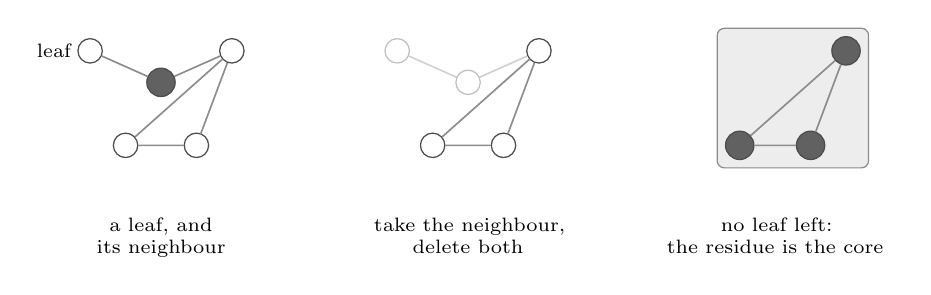
\begin{tikzpicture}[x=1cm,y=1cm]
% Leaf removal, three frames. A leaf's NEIGHBOUR is taken; both are deleted.
\foreach \f/\lab in {0/{a leaf, and\\ its neighbour},
                     1/{take the neighbour,\\ delete both},
                     2/{no leaf left:\\ the residue is the core}}{
  \node[lb,anchor=north,align=center,text width=3.0cm]
    at (\f*3.9+0.9,-1.25) {\lab};
}
% --- frame 1
\begin{scope}
  \node[nd] (p0) at (0,0.75) {};
  \node[hub] (q0) at (0.9,0.35) {};
  \node[nd] (r0) at (1.8,0.75) {};
  \node[nd] (s0) at (1.35,-0.45) {};
  \node[nd] (t0) at (0.45,-0.45) {};
  \draw[lnk] (p0)--(q0) (q0)--(r0) (r0)--(s0) (s0)--(t0) (t0)--(r0);
  \node[lb,anchor=east] at (-0.12,0.75) {leaf};
\end{scope}
% --- frame 2
\begin{scope}[xshift=3.9cm]
  \node[nd,draw=black!25] (p1) at (0,0.75) {};
  \node[nd,draw=black!25] (q1) at (0.9,0.35) {};
  \node[nd] (r1) at (1.8,0.75) {};
  \node[nd] (s1) at (1.35,-0.45) {};
  \node[nd] (t1) at (0.45,-0.45) {};
  \draw[lnk,draw=black!18] (p1)--(q1) (q1)--(r1);
  \draw[lnk] (r1)--(s1) (s1)--(t1) (t1)--(r1);
\end{scope}
% --- frame 3
\begin{scope}[xshift=7.8cm]
  \node[hub] (r2) at (1.8,0.75) {};
  \node[hub] (s2) at (1.35,-0.45) {};
  \node[hub] (t2) at (0.45,-0.45) {};
  \draw[lnk] (r2)--(s2) (s2)--(t2) (t2)--(r2);
  \begin{scope}[on background layer]
    \node[cx,fit=(r2)(s2)(t2)] {};
  \end{scope}
\end{scope}
\end{tikzpicture}
\end{adjustbox}
\caption{\textbf{Vertex covering leaf removal.} A vertex of degree one is a
leaf; some minimum cover contains its \emph{neighbour}, so the neighbour is
taken (dark) and both are deleted. Repeating consumes the graph, and if it
consumes all of it the cover produced is provably minimum. Here it does not: the
triangle has no leaf, and the residue is the core --- the structure on which the
algorithm has nothing to say, and which the rest of the chapter is about.}
\label{fig:leafremoval}
\end{figure}

\section{The core as an obstruction}
\label{sec:coreobstruction}
\index{core}
\index{core percolation|textbf}

Run leaf removal on the cavity branch and ask what a node reached along an
inclusion ends up as. There are three answers, not two: leaf-ready ($L$),
deleted ($D$), or core-side ($C$). Percolation had two answers and got a scalar;
this has three, and needs a message with three components.

The branch is Sec.~\ref{sec:cavity}'s construction. Take the inclusion of a node
$i$ into a complex $a$, remove $a$, and what still hangs off $i$ --- its other
complexes, and everything reachable through them --- is the cavity branch.
Running the algorithm there and nowhere else makes the outcome a property of the
branch alone, which is what lets it travel along the inclusion as a message.

The three states are the three things the branch can tell $a$
(Fig.~\ref{fig:cavitybranch}).
\emph{Leaf-ready}: the branch consumed itself and left $i$ holding nothing else,
so $i$ is a leaf as far as $a$ is concerned and $a$ may take it.
\emph{Deleted}: some other complex has already taken $i$, which is therefore
not there to be counted. \emph{Core-side}: the algorithm stalled on the branch
with $i$ still holding two or more live inclusions, and $a$ cannot resolve it.
The first two are both settled and they act on $a$ in opposite directions --- one
offers it a leaf, the other removes a member --- which is why they cannot be
collapsed into a single number the way percolation's two answers could.

The three-state cavity treatment of core percolation on graphs is due to
\citet{liu2012}, and is called the \emph{LCZP map} here, after Liu, Cs\'oka,
Zhou and P\'osfai. What follows carries it to complexes, so
Eq.~\eqref{eq:core} is the LCZP map on a chygraph. The letters here are
this book's: $\psi$ and $\delta$ are written $\alpha$ and $\beta$ in that paper
--- their $\alpha$-removable and $\beta$-removable --- and both letters are
spoken for elsewhere in this book, $\alpha$ being
Chapter~\ref{ch:satisfiability}'s clause density and $\beta$ the inverse
temperature throughout Part~III.

Writing $(\psi,\delta,\gamma)$ for the probabilities of the three states
--- leaf-ready, deleted, core --- the chy-degree step is
\begin{equation}
  \psi_{m}=\bar\Phi^{(m)}(\zeta),
  \qquad
  \delta_{m}=1-\bar\Phi^{(m)}(1-\xi),
  \label{eq:core}
\end{equation}
and the intra-complex step is solved exactly, as Sec.~\ref{sec:downstep} always
does. Two equations carry three states because the third is fixed by
normalisation, $\gamma_{m}=1-\psi_{m}-\delta_{m}$: a node is leaf-ready,
deleted, or --- failing both --- core-side. A branch with no core is therefore
$\psi+\delta=1$, which is the form Sec.~\ref{sec:corefree} puts to the map.

The two quantities it supplies, $\zeta$ and $\xi$, are what a complex does to a
node entering it. Enter a layer-$l$ complex through one member and look at the
other $c_{l}-1$. With $n$ of them still live, every live member has
clique-degree exactly $n$ inside the complex, so two events matter and no
others.

\emph{The complex leaves the entering node free to be a leaf} only when it
offers nothing at all --- when every one of the other $c_{l}-1$ members is
already deleted --- so $\zeta_{l}=\delta_{l}^{\,c_{l}-1}$.

\emph{The complex forces the entering node out} only when exactly one other
member is live and leaf-ready. With two or more live members the entering node
is not a leaf of that complex and the complex decides nothing. There are
$c_{l}-1$ ways to choose which member is the live one, so
$\xi_{l}=(c_{l}-1)\,\delta_{l}^{\,c_{l}-2}\psi_{l}$.

At $c_{l}=2$ these degenerate to $\zeta_{l}=\delta_{l}$ and $\xi_{l}=\psi_{l}$,
returning the graph recursion $\psi=\bar\Phi(\delta)$, $\delta=1-\bar\Phi(1-\psi)$. The whole of it
--- the three states, the two intra-complex quantities and the fixed point --- is
\code{Chygraph.\allowbreak core}, whose \code{solve} iterates monotonically from
zero because, unlike Eq.~\eqref{eq:vc}, this map is order-preserving; the
algebra is in \code{core.\allowbreak CorePercolation}.




\begin{figure}[t]
\centering
\begin{adjustbox}{max width=\linewidth}
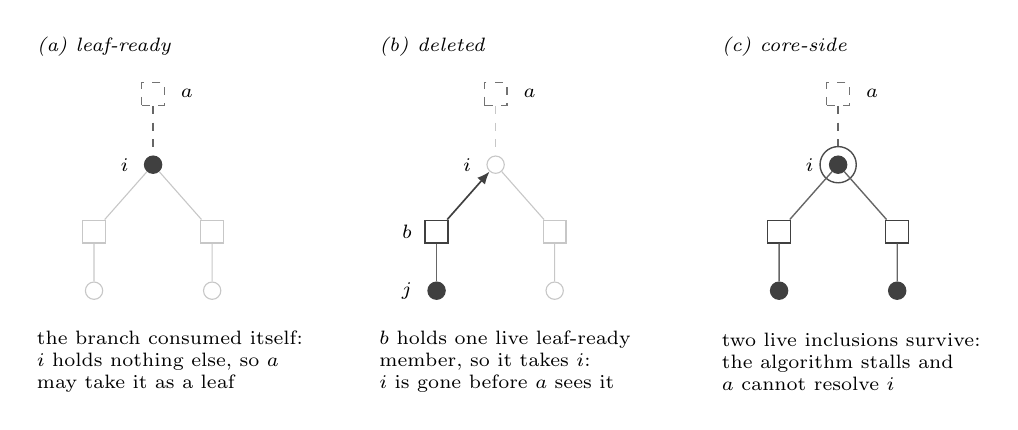
\begin{tikzpicture}[
  gone/.style={draw=black!22,fill=white,text=black!30},
  gonel/.style={draw=black!22},
]
% ============================= (a) leaf-ready
\begin{scope}
  \node[tb,anchor=west] at (-0.55,3.15) {(a) leaf-ready};
  \node[cpx,draw=black!55,dashed] (aA) at (1.05,2.55) {};
  \node[lb,anchor=west] at (1.28,2.55) {$a$};
  \node[atm] (iA) at (1.05,1.65) {};
  \node[lb,anchor=east] at (0.86,1.65) {$i$};
  \draw[incd] (aA)--(iA);
  \node[cpx,gone] (b1A) at (0.30,0.80) {};
  \node[cpx,gone] (b2A) at (1.80,0.80) {};
  \node[atm,gone,fill=white] (j1A) at (0.30,0.05) {};
  \node[atm,gone,fill=white] (j2A) at (1.80,0.05) {};
  \draw[gonel] (iA)--(b1A) (iA)--(b2A) (b1A)--(j1A) (b2A)--(j2A);
  \node[lb,anchor=west,align=left] at (-0.55,-0.85)
    {the branch consumed itself:\\ $i$ holds nothing else, so $a$\\ may take it as a leaf};
\end{scope}
% ============================= (b) deleted
\begin{scope}[xshift=4.35cm]
  \node[tb,anchor=west] at (-0.55,3.15) {(b) deleted};
  \node[cpx,draw=black!55,dashed] (aB) at (1.05,2.55) {};
  \node[lb,anchor=west] at (1.28,2.55) {$a$};
  \node[atm,gone,fill=white] (iB) at (1.05,1.65) {};
  \node[lb,anchor=east] at (0.86,1.65) {$i$};
  \draw[incd,gonel] (aB)--(iB);
  \node[cpx] (b1B) at (0.30,0.80) {};
  \node[lb,anchor=east] at (0.11,0.80) {$b$};
  \node[cpx,gone] (b2B) at (1.80,0.80) {};
  \node[atm] (j1B) at (0.30,0.05) {};
  \node[lb,anchor=east] at (0.11,0.05) {$j$};
  \node[atm,gone,fill=white] (j2B) at (1.80,0.05) {};
  \draw[inc] (b1B)--(j1B);
  \draw[gonel] (iB)--(b2B) (b2B)--(j2B);
  \draw[msg] (b1B) -- (iB);
  \node[lb,anchor=west,align=left] at (-0.55,-0.85)
    {$b$ holds one live leaf-ready\\ member, so it takes $i$:\\ $i$ is gone before $a$ sees it};
\end{scope}
% ============================= (c) core-side
\begin{scope}[xshift=8.7cm]
  \node[tb,anchor=west] at (-0.55,3.15) {(c) core-side};
  \node[cpx,draw=black!55,dashed] (aC) at (1.05,2.55) {};
  \node[lb,anchor=west] at (1.28,2.55) {$a$};
  \node[atm] (iC) at (1.05,1.65) {};
  \node[lb,anchor=east] at (0.86,1.65) {$i$};
  \draw[incd] (aC)--(iC);
  \node[circle,draw=black!70,line width=.5pt,minimum size=4.6mm,inner sep=0pt]
        at (1.05,1.65) {};
  \node[cpx] (b1C) at (0.30,0.80) {};
  \node[cpx] (b2C) at (1.80,0.80) {};
  \node[atm] (j1C) at (0.30,0.05) {};
  \node[atm] (j2C) at (1.80,0.05) {};
  \draw[inc] (iC)--(b1C) (iC)--(b2C) (b1C)--(j1C) (b2C)--(j2C);
  \node[lb,anchor=west,align=left] at (-0.55,-0.85)
    {two live inclusions survive:\\ the algorithm stalls and\\ $a$ cannot resolve $i$};
\end{scope}
\end{tikzpicture}
\end{adjustbox}
\caption{\textbf{The cavity branch and the LCZP map.} Drawn
as inclusions in the vocabulary of Sec.~\ref{sec:drawing}: filled circles are
atoms, rectangles complexes, a line is membership. In each panel the complex
$a$ is the one arrived through and is removed --- drawn dashed --- and what
hangs below $i$ is the cavity branch. Leaf removal is run on that branch and
nowhere else, which is what makes the outcome a property of the branch and so a
message on the inclusion $i\to a$. Pale grey is what the algorithm has already
stripped. The three outcomes are not two: (a) and (b) are both settled and act
on $a$ in opposite directions, one offering it a leaf and the other removing a
member, which is why the LCZP map carries three numbers where
Chapter~\ref{ch:percolation} carried one.}
\label{fig:cavitybranch}
\end{figure}

Unlike Eq.~\eqref{eq:hs} this map is order-\emph{preserving}, so monotone
iteration from zero suffices and none of Sec.~\ref{sec:hard}'s bracketing
apparatus is needed. That is the distinction Sec.~\ref{sec:fixedpoint} drew, put
to use: the two maps live on the same chygraph and differ in the signs of their
entries, and the sign decides which solver applies.

\paragraph{The branch is a device and not a step of the algorithm.} Leaf removal
does not remove a complex and restart; it peels the whole object at once, and
Sec.~\ref{sec:leafremoval}'s rule never mentions a cavity. What the branch does
is turn that global peeling into a local recursion, and it is exactly where the
treelike assumption enters: cutting $a$ is taken to leave the rest of $i$'s
neighbourhood self-contained. Where it does not --- where the branch closes on
itself by some other route --- the LCZP map is predicting the output of an
algorithm that will not do what the recursion says, and the algorithm is the one
that is right, since Sec.~\ref{sec:leafremoval}'s exchange argument holds on any
graph. Sections~\ref{sec:hrg} and~\ref{sec:realcore} measure the size of that
gap; it is the whole of the difference between their measured and chygraph
columns.

\section{On a graph: one point, three names}
\label{sec:onepoint}

At $c=2$ the LCZP map has threshold $\bar\Phi'(1-\psi)=1$, which for
Poisson chy-degree is
\begin{equation}
  \ave{k}=e.
\end{equation}
Below it the core is empty and leaf removal certifies a minimum cover; above it
the core is extensive and the algorithm stalls. This is the Bauer--Golinelli
threshold \citep{bauer2001}.

It is also Eq.~\eqref{eq:kc} at $c=2$: the loss of stability of
Chapter~\ref{ch:hittingset}'s hard-field map. And it is the accepted
replica-symmetry-breaking point for vertex cover on Poisson graphs
\citep{weigt2000}. Computed independently, the first two agree to
$2.5\times10^{-10}$, which is a consistency check rather than a coincidence:
they are the same point reached by two routes.


In words, and this is why the three subjects share a chapter. \emph{Leaf removal certifies a
cover exactly when there is no core; there is no core exactly when the
hard-field map is stable; and the hard-field map is stable exactly where the
integer messages carry the whole answer.} Three statements, one condition.

\paragraph{Over several layers.} The threshold above is the one-layer form,
and the general one is worth writing down because three of
Fig.~\ref{fig:mappings}'s five structures carry more than one layer. The
core-free branch is a \emph{vector}, $\psi_{m}=\bar\Phi^{(m)}(1-\psi)$ with one
entry per layer, since a node reached along a layer-$m$ inclusion is
size-biased in layer $m$ alone and two layers share a $\psi$ only when they are
statistically alike. Linearising Eq.~\eqref{eq:core} there gives a Jacobian
$\bigl(\begin{smallmatrix}0&A\\A&0\end{smallmatrix}\bigr)$ --- at $c=2$ the
$\psi$ row moves only with $\zeta=\delta$ and the $\delta$ row only with
$\xi=\psi$ --- so its spectrum is $\pm$ that of
\begin{equation}
  A_{ml}=\frac{\partial\bar\Phi^{(m)}}{\partial x_{l}}\bigg|_{x=1-\psi},
  \qquad\text{and the core appears at}\quad \rho(A)=1.
  \label{eq:corethresh}
\end{equation}
Those eigenvalues are real: $A_{ml}$ is $\partial^{2}\Phi/\partial
x_{m}\partial x_{l}$, symmetric, divided by the mean layer-$m$ chy-degree. At
$L=1$ it is $\bar\Phi'(1-\psi)=1$ again. This is
\code{core\_\allowbreak free\_\allowbreak spectral}.

For Poisson layers it collapses much further. Every $\bar\Phi^{(m)}$ is then
$\Phi$ itself, so $\psi$ is common to the layers and $A_{ml}=\kappa_{l}\psi$
does not depend on $m$: $A$ has rank one, $\rho(A)=\psi\sum_{l}\kappa_{l}$, and
with $\psi=e^{-\psi\sum_{l}\kappa_{l}}$ the threshold is
\begin{equation}
  \sum_{l}\kappa_{l}=e.
  \label{eq:sumkappae}
\end{equation}
The \emph{total} chy-degree, however it is split. So the multiplex and the
interacting graphs of Fig.~\ref{fig:mappings} sit at the graph's own threshold
rather than somewhere else, and adding a link type moves nothing;
Eq.~\eqref{eq:sumkappae} is checked against Eq.~\eqref{eq:corethresh} to
$2\times10^{-10}$ at one, two, three and five layers. Layers move the point only
when they differ in \emph{shape} and not merely in mean. A multiplex of a
diluted matching layer and a Poisson layer cores at total $\ave{k}=2.6196$,
against $2.6994$ for the single graph with the same pooled degree distribution
--- the difference being the degree correlation multiplexing imposes on the
matching layer's own links, which pooling destroys.

\paragraph{Which replica-symmetry-breaking point.} The first of
Sec.~\ref{sec:onestep}'s two, and it is worth being explicit because the
distinction costs a chapter elsewhere. This is where the solution space
\emph{shatters} --- where clusters appear and the core along with them --- and
not where minimum covers run out; covers exist on both sides of $e$, and what
changes is whether they form one cluster or many. Locating it here needs no
survey: the core is a percolation problem and the LCZP map solves it by
algebra. Section~\ref{sec:colouring-sp} reaches the same class of point for
colouring by the other route, as the density at which its surveys stop being
trivial, and pays a population dynamics for it.

What lies past $e$ this chapter does not compute. That is the complexity of
Eq.~\eqref{eq:sigmagen}, and Chapters~\ref{ch:colouring}
and~\ref{ch:satisfiability} are where the book carries it out --- for colouring
and satisfiability, not for this family, whose own one-step answer
Sec.~\ref{sec:hsrsb} states the cost of and leaves open.

\section{Above cardinality two the core-free branch disappears}
\label{sec:corefree}
\index{core}

Raising the cardinality changes the picture abruptly.

A core-free branch means $\gamma=0$, that is $\psi+\delta=1$. Substituting
Eq.~\eqref{eq:core},
\[
  \bar\Phi^{(m)}(\zeta)+1-\bar\Phi^{(m)}(1-\xi)=1,
\]
and since $\bar\Phi$ is a power series with non-negative coefficients, hence
strictly increasing, this requires $\zeta=1-\xi$ in every layer. With
$\psi=1-\delta$ that is
\[
  f(\delta)\equiv(c-1)\delta^{\,c-2}-(c-2)\delta^{\,c-1}-1=0.
\]
The polynomial factors, and the factorisation is the whole argument:
\begin{equation}
  f(\delta)=-(1-\delta)^{2}\sum_{j=0}^{c-3}(j+1)\,\delta^{\,j}.
  \label{eq:factored}
\end{equation}
At $c=2$ the sum is empty and $f\equiv0$: the condition is an \emph{identity},
and the core-free branch exists at every chy-degree below threshold. At $c\ge3$
every coefficient of the sum is strictly positive, so $f(\delta)<0$ on $[0,1)$
and $f(1)=0$. The only root is $\delta=1$, forcing $\psi=0$. The predicate is \code{has\_\allowbreak core\_\allowbreak free\_\allowbreak branch} on
that same object, and it returns true exactly when every cardinality is two.

So a chygraph carrying any layer of cardinality three or more has no core-free
branch at all, at any density. Leaf removal never certifies a cover there.

Figure~\ref{fig:core} draws it. At $c=2$ there is a transition at $e$; at $c=3$
and above there is no transition, and the two curves lie exactly on top of each
other because for a pure clique network of cardinality three or more the core is
$1-e^{-\ave{k}}$ --- every vertex that is in any complex at all. Cardinality
past three changes nothing: the obstruction is not a matter of degree.

\begin{figure}[t]
\centering
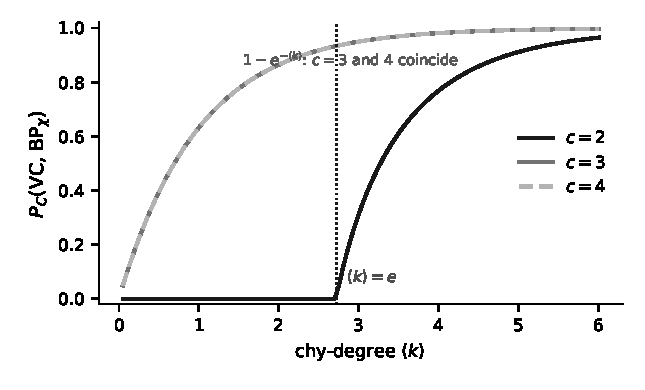
\includegraphics[width=0.88\linewidth]{figs/fig-core.pdf}
\caption{\textbf{The core-free branch and its disappearance.} Core fraction
$P_{C}(\mathrm{VC},\chi)$ --- take a chy-degree-one atom together
with the complex holding it, and what survives is the core --- against
chy-degree, for pure clique networks. At cardinality two there is a
transition at $\ave{k}=e$, below which the core is empty and leaf removal
certifies a minimum cover. At cardinality three and above there is no
transition: Eq.~\eqref{eq:factored} forbids the core-free branch, and the core
is $1-e^{-\ave{k}}$, every non-isolated vertex. The $c=3$ and $c=4$ curves
coincide exactly. Generated by \code{figs/\allowbreak cover.\allowbreak py}.}
\label{fig:core}
\end{figure}

This closes a loop. Section~\ref{sec:hardfail} said the hard-field cover size is
exact at cardinality two and an approximation above it, and appealed to
certification without proving it. Equation~\eqref{eq:factored} is the proof, and
it is a property of the LCZP map rather than an assumption imported from
elsewhere: the cover size of Eq.~\eqref{eq:hs} can be believed exactly when
the LCZP map admits $\gamma=0$, and both hold only at $c=2$.

\paragraph{A reading to block.} The result does \emph{not} say that a complex
survives leaf removal whole. Leaf removal deletes a leaf's \emph{neighbour}, and
a triangle carrying one pendant edge per vertex has an empty core. What the
algebra gives is only that the core cannot vanish identically --- not that it is
large. Add a triangle layer of chy-degree $10^{-3}$ to a Poisson link layer of
chy-degree $1$ and the predicted core is $1.8\times10^{-4}$: non-zero, as
Eq.~\eqref{eq:factored} requires, and of no practical consequence whatever. The
statement is about a branch of a fixed point, and a statement about a branch is
not a statement about a magnitude.

\paragraph{How small, exactly.} The magnitude has a closed form, and it is
worth having because Sec.~\ref{sec:realcore} meets it four times in data. Put a
clique layer of cardinality $c$ and chy-degree $\kappa_{c}$ on a link layer and
expand Eq.~\eqref{eq:core} to first order in $\kappa_{c}$. Writing $\psi_{0}$
for the link layer's own leaf-ready probability, $\psi_{0}=\bar\Phi(1-\psi_{0})$,
and $\delta_{0}=1-\psi_{0}$,
\begin{equation}
  P_{C}(\mathrm{VC},\chi)\simeq\kappa_{c}\,\psi_{0}
    \Bigl[1-\delta_{0}^{\,c-1}-(c-1)\,\psi_{0}\,\delta_{0}^{\,c-2}\Bigr].
  \label{eq:smallcore}
\end{equation}
The bracket is $1-\zeta-\xi$ evaluated on the link background: the chance that
the clique neither leaves the entering node free nor deletes it, which is the
chance it leaves it core-side. At $c=2$ it is zero identically, as it must be,
and at $c=3$ the whole expression is $\kappa_{\triangle}\psi_{0}^{3}$ --- one
triangle in the core exactly when all three of its branches are leaf-ready,
which is the combinatorial statement one would write down directly. At link
chy-degree $1$ and $\kappa_{\triangle}=10^{-3}$ it gives $1.824\times10^{-4}$,
the number quoted above.

Two things follow, and they are the point of writing it out. The core is
\emph{linear} in the clique density with a bounded slope, so
Eq.~\eqref{eq:factored} constrains a slope and not a magnitude --- which is the
previous paragraph, now with a coefficient. And Eq.~\eqref{eq:smallcore} does
not diverge at $\ave{k}=e$. The cavity $\gamma$ does, carrying a factor
$1/[1-\bar\Phi'(1-\psi_{0})]$, but the core fraction multiplies it by the same
factor and the two cancel exactly. So the transition a link layer has at $e$
does not turn into a divergence when a few triangles are added to it. It turns
into nothing at all, and Eq.~\eqref{eq:smallcore} passes through $e$ without
registering it.

\paragraph{Where the three names separate.} Section~\ref{sec:onepoint}'s
identification is a statement about $c=2$, and above $c=2$ its three names come
apart. The core has no threshold at all, which is what
Eq.~\eqref{eq:factored} has just said. The two hard-field maps still have one
each, and those two are no longer the same point either. Eliminating
$\kappa$ between the Poisson fixed point of Eq.~\eqref{eq:vc},
$\sigma=e^{\kappa(u^{c-1}-1)}$ with $u=1-\sigma$, and its instability
$\kappa(c-1)\sigma u^{c-2}=1$ leaves one transcendental equation in $\sigma$
alone:
\begin{equation}
  \ln\sigma=\frac{u^{\,c-1}-1}{(c-1)\,\sigma\,u^{\,c-2}},
  \qquad
  \ave{k}_{c}=\frac{1}{\sigma\,u^{\,c-2}},
  \label{eq:vcinstab}
\end{equation}
where $\ave{k}_{c}=\kappa(c-1)$ is the induced mean degree. It returns $e$ at
$c=2$, and then $4.7836$, $7.0871$, $9.5736$ at $c=3,4,5$: covering a clique
network gets harder, in neighbours per node, as the cliques grow. Read the same
way Chapter~\ref{ch:hittingset} reads Eq.~\eqref{eq:kc}, the hitting-set point
does not move at all --- $\ave{k}(c-1)=e$ for every cardinality. So the two
instabilities coincide at $c=2$ and separate immediately above it, and three
names for one point is precisely what cardinality two buys.

\section{Structured networks}
\label{sec:fivecover}

Chapter~\ref{ch:chygraphs} claimed that a calculation done once on a chygraph
is a calculation done for all five structures of Fig.~\ref{fig:mappings}, and
that specialising it is substitution rather than rederivation. The chapter is
now far enough along to pay that out. Section~\ref{sec:hsfive} does the same
for hitting set, and the two lists do not split alike: that section says where
they differ and why. What follows is the five, in
Sec.~\ref{sec:everything}'s order and under its names. None of it is a new
calculation: every entry is Eq.~\eqref{eq:vc} or Eq.~\eqref{eq:core} with a
list of cardinalities substituted, and Table~\ref{tab:five} is what comes back.

One number decides the whole table. Equation~\eqref{eq:factored} says the
core-free branch survives exactly when every layer has cardinality two, so the
five split two against three, and which side a structure falls on is a property
of its layer list and of nothing else --- not of its density, not of its degree
distribution, not of how many layers it carries.

\begin{table}[t]
\centering\small
\begin{adjustbox}{max width=\linewidth}
\begin{tabular}{lccrrc}
\hline\hline
structure & $c$ & threshold & $P_{C}$ & cover & certified\\
\hline
A graph & $2$ & $\ave{k}=e$ & 0.0000 & 0.3920 & yes\\
A hypergraph & $3$ & none & 0.6321 & 0.3426$^{*}$ & no\\
A multiplex network & $2,2$ & $\ave{k}=e$ & 0.0000 & 0.3920 & yes\\
Interacting graphs & $2,2,2$ & $\ave{k}=e$ & 0.0000 & 0.3920 & yes\\
Interacting hypergraphs & $3,3,3$ & none & 0.6321 & 0.3426$^{*}$ & no\\
A clustered graph & $2,3$ & none & 0.1287 & 0.3704$^{*}$ & no\\
\hline\hline
\end{tabular}

\end{adjustbox}
\caption{\textbf{The three methods on the structures of
Fig.~\ref{fig:mappings}.} All six rows at one induced mean degree,
$\ave{k}=2$, below the graph's own threshold $e$. A layer-$l$ complex supplies
$c_{l}-1$ neighbours per member, so $\ave{k}=\sum_{l}\kappa_{l}(c_{l}-1)$ is
what is held fixed; the chy-degree is split evenly across the layers and
Poisson in each. $P_{C}$ is the core fraction of Eq.~\eqref{eq:core} and
\emph{cover} the size of Eq.~\eqref{eq:vc}; a star marks a cover size leaf
removal does not certify, where Sec.~\ref{sec:corefree} says it never will and
\code{cover\_\allowbreak bracket} is the honest statement. The three
cardinality-two rows agree to every digit shown, which is
Eq.~\eqref{eq:sumkappae}. Generated by
\code{figs/\allowbreak cover.\allowbreak py:table\_\allowbreak five\_\allowbreak structures}.}
\label{tab:five}
\end{table}

\paragraph{A graph} is one layer of links. One layer of cardinality two puts
$A$ of Eq.~\eqref{eq:corethresh} at $1\times1$, so $\rho(A)$ is
$\bar\Phi'(1-\psi)$ and the core appears at $\ave{k}=e$ for Poisson degree.
For example, the row is a Poisson link layer at chy-degree two, below that and
so core-free. It is the row the others are read against: all three methods
work and agree: Eq.~\eqref{eq:vc} returns the Weigt--Hartmann cover size, leaf
removal certifies it below $\ave{k}=e$, and Sec.~\ref{sec:onepoint}'s three
names are one point. Nothing here is new, and that is what makes it the
baseline.

\paragraph{A hypergraph} is one complex layer with the cardinality free. Where
it carries a single size $c\ge3$, Eq.~\eqref{eq:factored} removes the core-free
branch, so there is no threshold
to write down at all; the core is instead $1-\Phi(0)$ at every density. For
example, the row is a Poisson layer of $3$-cliques at chy-degree one, the same
two neighbours per node as the graph, and its core is $1-e^{-1}=0.6321$, which is the table's entry. The
structure loses everything the graph had at once, and the loss is structural
rather than a matter of density. Note first which problem is being solved: this
chapter covers the \emph{induced} graph, so a hyperedge is a clique and every
pair inside it must be covered. Hitting the hyperedges themselves is
Chapter~\ref{ch:hittingset}'s problem with the other constraint,
Eq.~\eqref{eq:Hvc} against Eq.~\eqref{eq:Hhs}. Then, at cardinality three or
more, no vertex of a clique ever has degree one, so leaf removal never fires at
all: the core is the whole of $1-\Phi(0)$, every non-isolated vertex, at every
density. This is the strong reading of Sec.~\ref{sec:corefree} in the one place
where it does hold, which is where \emph{every} layer is above cardinality two.
Equation~\eqref{eq:vc}'s cover size is then an approximation with nothing to
certify it, and the row carries a star.

\paragraph{A multiplex network} is $L$ link layers on the same vertices. Every
layer is at $c=2$, so the core-free branch survives whatever $L$ is, and for
Poisson layers $A_{ml}=\kappa_{l}\psi$ has rank one and
Eq.~\eqref{eq:sumkappae} puts the threshold at $\sum_{l}\kappa_{l}=e$. For
example, the row is two Poisson link layers at chy-degree one each, total
chy-degree two. What the extra
layers do change is where the point sits, and the answer is nowhere:
Eq.~\eqref{eq:sumkappae} puts the threshold at the \emph{total} chy-degree $e$
for Poisson layers, so a multiplex of five sparse layers cores exactly where the
single graph carrying their sum does. That is why the three cardinality-two rows
of Table~\ref{tab:five} are the same row. Layers earn their keep only when they
differ in shape, where Eq.~\eqref{eq:corethresh}'s matrix is needed and the
pooled graph gets the point wrong.

\paragraph{Interacting graphs and hypergraphs} is $L$ layers whose
cardinalities need not agree, and the rule is the whole list: a core-free branch
survives when every $c_{l}=2$ and not otherwise. For example, the two rows are
three link layers at chy-degree $2/3$, which keeps it, and three layers of
$3$-cliques at chy-degree $1/3$, which does not. It is the panel that can land
on either side, and the layer list decides which. As Fig.~\ref{fig:mappings} draws
it --- cardinality two throughout, including the cross layer --- it is a
multiplex as far as this chapter is concerned, and the previous paragraph
applies unchanged. Interacting \emph{hypergraphs} put their own layers at
cardinality three or more and it is lost, whatever the cross layer does. So is
the converse case, two graphs interacting through a cross layer of hyperedges of
size three or more: the cross layer alone is enough. Both readings are in the
table because the distinction between them is the whole content of the panel.

\paragraph{A clustered graph} is a link layer together with one layer per clique
size present. One layer above cardinality two is enough for
Eq.~\eqref{eq:factored},
so there is no core-free branch and no threshold; what there is instead is
Eq.~\eqref{eq:smallcore}, the core linear in the clique chy-degree. For
example, the row is a Poisson link layer at chy-degree one beside a Poisson
triangle layer at chy-degree one half. It is formally on the bad side and is the
interesting one. It is the mapping Part~III rests on, and the mapping
Secs.~\ref{sec:hrg} and~\ref{sec:realcore} spend two sections measuring. Its
triangle layer sits at $c=3$, so Eq.~\eqref{eq:factored} removes the core-free
branch and leaf removal certifies nothing at any density. What
Eq.~\eqref{eq:smallcore} adds is the price: the core is linear in the triangle
chy-degree with a bounded slope, so a sparse link layer carrying a few triangles
has a core of order $10^{-4}$ and is, to any measurement, the graph of the first
paragraph. Table~\ref{tab:five}'s row is at triangle chy-degree $0.5$, which is
not a few, and its core is $0.129$. The distance between $10^{-4}$ and $0.129$
is what the clustered mapping is for, and Sec.~\ref{sec:realcore} finds both
ends of it in data: four networks where the prediction is $10^{-4}$ and leaf
removal finds nothing, five where it is per cent and leaf removal finds them.

\paragraph{What the list establishes.} Not that the five behave alike. They do
not, and Table~\ref{tab:five} is mostly a table of differences --- two of the
six rows certify nothing, and one of those is the row the rest of the book
cares about most. What the list establishes is
Chapter~\ref{ch:chygraphs}'s narrower claim, which is that the differences are
all substitutions. Six rows, one map, one solver, and the only thing that
changes from row to row is a list of integers.

\section{Hyperbolic random graphs}
\label{sec:hrg}
\index{hyperbolic random graph}

Everything so far is internal. Here the construction meets a network that was
not built to suit it; Sec.~\ref{sec:realcore} then meets sixteen that nobody
built at all.

Hyperbolic random graphs are the standing example of a clustered ensemble: they
have a heavy-tailed degree distribution and a great deal of clustering, both
induced by the geometry rather than imposed. Run leaf removal on one and it
finds an extensive core at \emph{every} mean degree, down to $\ave{k}=0.05$,
with no transition. Run it on the degree-matched configuration model --- same
degree distribution, same assortativity to within a few per cent --- and there is
no core at all until $\ave{k}$ reaches $4.5$ to $10$. Whatever separates them is
not in $\{p_{d},e_{dd'}\}$, and that gap is the motivation
Chapter~\ref{ch:introduction} opened with.

The chygraph treatment is: take the maximal cliques of the graph as complexes,
\emph{measure} the chy-degree ensemble from the graph itself, and evaluate
the LCZP map. Nothing is fitted. That is run over three decades in density,
$\ave{k}=0.05$ to $6$, at $n=2\times10^{5}$ and two seeds per point, against
leaf removal on the graph itself and against the degree-matched configuration
model. Data from
\code{statmech/\allowbreak probe/\allowbreak prediction4.\allowbreak py}.

\paragraph{What it gets right.} The qualitative separation is complete: the
chygraph has a core everywhere the real graph does, and the degree-matched
control has none. Quantitatively the chygraph accounts for $77$ to $100$ per
cent of the measured core, the shortfall tracking the clique overlap --- small
in a sparse graph, irrelevant once almost everything is core, worst in between.
And the core is a power law, $\mathrm{core}\sim\ave{k}^{\,\theta}$, with the
predicted exponent matching the measured one to $0.04$ at $\tau=2.5$ and $0.06$
at $\tau=2.9$.

\paragraph{The control that isolates the map.} There is one place
where the configuration model \emph{does} have a core: $\tau=2.9$, $\ave{k}=6$.
There the chygraph predicts $0.633$ against a measured $0.621$, two per cent ---
same map, same pipeline, and cliques that barely overlap at that density. So the
deficit on the hyperbolic graph at the same density is overlap, and not the map.
That comparison separates two things that would otherwise be confounded:
whether the LCZP map is right, and whether treating complexes as
independent is. It says the map is right and the independence is not, which is
exactly the diagnosis Chapter~\ref{ch:overlap} takes up.

\begin{figure}[tbp]
\centering
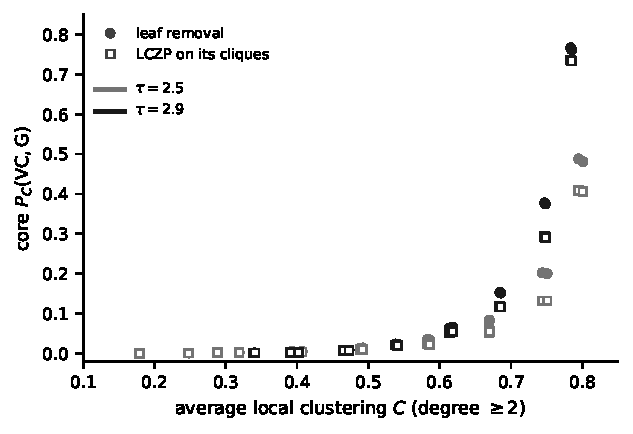
\includegraphics[width=\linewidth]{figs/fig-hrg-c.pdf}
\caption{\textbf{Vertex cover core size of hyperbolic random graphs.} The
leaf-removal core of hyperbolic random graphs against their own clustering,
both tails in one panel and both axes linear, $n=2\times10^{5}$ and two seeds
per point. Filled circles are leaf removal run on the graph; open squares are
the LCZP map evaluated on the maximal-clique ensemble measured from that same
graph, so nothing is fitted. The abscissa is the average local clustering over
vertices of degree at least two, which is where a triangle is possible at all:
these graphs are almost all isolated vertices at the sparse end --- under half
a per cent have two neighbours at $\ave{k}=0.05$ --- so the unrestricted mean
would report the density and call it clustering. The degree-matched
configuration model is not plotted: it sits at $C\le0.017$, off the left of the
axis, and has no core anywhere except at $\ave{k}=6$, $\tau=2.9$; the text
gives its numbers. Transitivity was tried
first and is not usable here: on a $\tau=2.5$ tail a few hubs of degree
$10^{3}$ set its denominator, and it comes out flat in $\ave{k}$ and split by
seed. Data from
\code{statmech/\allowbreak probe/\allowbreak hrg\_\allowbreak transitivity.\allowbreak py}
joined to
\code{statmech/\allowbreak probe/\allowbreak prediction4.\allowbreak py};
generated by
\code{figs/\allowbreak cover.\allowbreak py:figure\_\allowbreak hrg\_\allowbreak c}.}
\label{fig:hrgc}
\end{figure}

\paragraph{What the figure is drawn against.} Mean degree is the knob, and
Fig.~\ref{fig:hrgc} is drawn against what the knob produces instead, because
the separation this section is about is a separation in \emph{structure}. Every
hyperbolic graph in it sits between $C=0.18$ and $0.80$; every degree-matched
control sits at $C\le0.017$, which is why the control is not plotted --- on a
linear axis it would be a column of points on the ordinate.
What is plotted is the comparison that could have failed: the LCZP prediction
against the measurement, over the whole range, and the open squares follow the
filled circles at every clustering, recovering $64$ to $85$ per cent of the
measured core at $\tau=2.5$ and $77$ to $100$ at $\tau=2.9$. The gap is the
overlap deficit and it does not grow with $C$.

Two cautions come with it. Clustering is not a control here: it is produced by
$\ave{k}$, rising monotonically with it because a denser hyperbolic graph has
more vertices with two neighbours to be clustered, so this is a
reparametrisation of the density sweep and not an independent one. And at
$\ave{k}=6$ the control has a core of its own, $0.62$ at $C\approx0$ --- density
alone makes one, the point Sec.~\ref{sec:realcore} makes again on real
networks, and a reminder that the abscissa does not order the physics by
itself.

\paragraph{How much this establishes.} Less than it looks.
Section~\ref{sec:corefree} shows that \emph{any} layer of
cardinality three or more removes the core-free branch, so a positive prediction
follows from the algebra the moment one triangle enters the ensemble, whatever
else the graph is doing. The existence of the core was never in doubt once the
mapping was chosen.

The exponent is the part that could have failed. And there the evidence is
weaker than the central values suggest. Bootstrapped over seeds, the predicted
exponent does not move with $\tau$ at all --- $1.57$, $1.55$, $1.57$ at
$\tau=2.1$, $2.5$, $2.9$ --- while the measured one spreads by seven times as
much and rises monotonically with the tail, $1.49$, $1.59$, $1.64$. The two
agree within errors at $\tau=2.5$ and differ at $\tau=2.9$ by roughly four standard
deviations. What the comparison establishes is that the chygraph produces a
power law of about the right exponent; not that it tracks the exponent's
dependence on the tail. A sharper test would need an ensemble in which the
predicted exponent is made to move, and an analytic account of what fixes it
near $1.57$ in the LCZP map. Neither is attempted here, and both are on
Chapter~\ref{ch:outlook}'s list.

\section{Graphs with degree correlations}
\label{sec:vw}
\index{degree correlations}

Section~\ref{sec:hrg} ended on the claim that whatever separates the hyperbolic
graph from its degree-matched control is not in $\{p_{d},e_{dd'}\}$. That is a
statement about a description, and it is worth knowing what that description
\emph{can} do before concluding it cannot do this. It can do a great deal. Run
vertex cover over the full node-and-link ensemble --- arbitrary degree
distribution, arbitrary correlation between the degrees at the two ends of a
link --- and there is a phase transition along the correlation axis alone, with
the degree distribution held exactly fixed. It is due to \citet{vazquez2003vw},
and it is recapitulated here for two reasons. It fixes what the node-and-link
description is capable of, which Sec.~\ref{sec:hrg} needs in order to say that
the hyperbolic graph and its control are not separated by it. And it is this
chapter's own map, refined on a different index.

\paragraph{The ensemble.} Fix $p_{d}$, and with it the excess-degree
distribution $q_{d}=(d+1)p_{d+1}/\ave{k}$. Then fix, independently, the
symmetric joint distribution $e_{dd'}$ of the excess degrees at the two ends of
a link, subject only to $\sum_{d'}e_{dd'}=q_{d}$, so that the conditional
$p(d'|d)=e_{dd'}/q_{d}$ is what a walker arriving at a vertex of excess degree
$d$ sees on the other side. Uncorrelated graphs are the single point
$e_{dd'}=q_{d}q_{d'}$; everything else on that simplex is a correlated graph
with the \emph{same} degree distribution. This is the largest ensemble whose
atoms are nodes and links, and no further refinement of that vocabulary reaches
past it.

\paragraph{What it costs.} A Bethe--Peierls treatment on such a graph no longer
closes on one cavity-field distribution. It closes on one \emph{per excess
degree}, $P_{d}(h)$, coupled through $p(d'|d)$, because two vertices of the same
degree stop being statistically alike once the degrees of their neighbours
differ. In the $\mu\to\infty$ limit --- the hard-field limit of
Sec.~\ref{sec:hard}, and the same discard Sec.~\ref{sec:hardfail} shows is
harmless on a graph and fatal above cardinality two --- those distributions
collapse onto integers, and one scalar per degree class survives:
\begin{equation}
  \pi_{d}=\sum_{d'}\frac{e_{dd'}}{q_{d}}\,(1-\pi_{d'})^{\,d'},
  \label{eq:vwpi}
\end{equation}
with $\pi_{d}$ the probability that a link entering a vertex of degree $d+1$ is
not already covered from the other end. The cover size follows,
\begin{equation}
  x_{c}=1-p_{0}-\sum_{d\ge1}p_{d}\,(1-\pi_{d-1})^{\,d-1}
        \Bigl(1+\frac{d-2}{2}\,\pi_{d-1}\Bigr).
  \label{eq:vwxc}
\end{equation}

Equation~\eqref{eq:vwpi} is Eq.~\eqref{eq:vc} with the index moved. This
chapter resolves the one scalar $\sigma$ by \emph{layer}, because a node reached
along a layer-$m$ inclusion is size-biased in layer $m$ alone;
Eq.~\eqref{eq:vwpi} resolves it by \emph{degree class}, because a link entering
a vertex of excess degree $d$ lands on a neighbourhood biased by $p(d'|d)$. Two
refinements of one map, on two indices, and they are orthogonal: neither
reaches the other. Both are order-reversing, so both need Sec.~\ref{sec:hard}'s
bracket rather than plain iteration, and it was on this map that the
oscillation was first noticed and read as the physical signal it is.

At $e_{dd'}=q_{d}q_{d'}$ the sum in Eq.~\eqref{eq:vwpi} loses its $d$
dependence and the whole thing is one scalar again. For Poisson $p_{d}$ that
scalar is Sec.~\ref{sec:twoconstraints}'s: Eq.~\eqref{eq:vwxc} returns the
Weigt--Hartmann size to machine precision at $\ave{k}=1,2,3,5,10$, and its
instability sits at $\ave{k}=e$ to fifteen digits. Section~\ref{sec:onepoint}'s
one point with three names is the uncorrelated Poisson corner of this ensemble.

\begin{figure}[tbp]
\centering
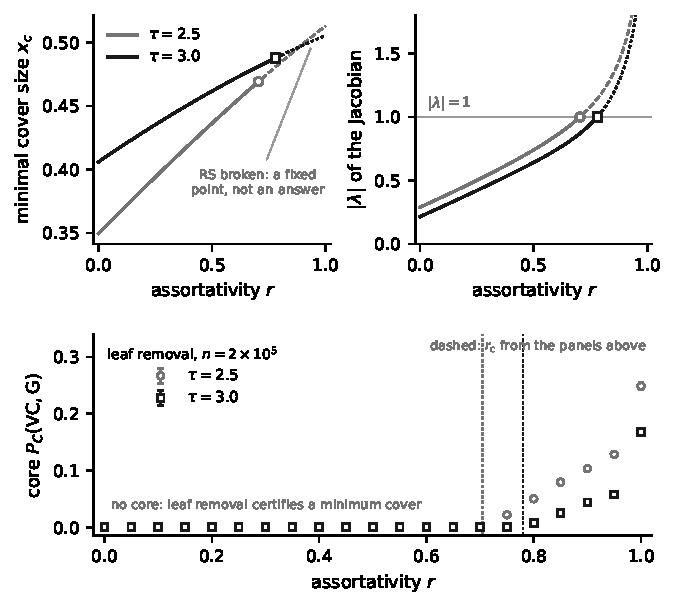
\includegraphics[width=\linewidth]{figs/fig-vw.pdf}
\caption{\textbf{Phase transition in degree correlated graphs.} Along the
assortativity axis of Eq.~\eqref{eq:vwr}, at $p_{d}\sim d^{-\tau}$ held
\emph{exactly} fixed: only $e_{dd'}$ moves. \emph{Top left}, the cover size,
solid where the fixed point of Eq.~\eqref{eq:vwpi} is stable and dashed past
$r_{\mathrm{c}}$ where it is a fixed point and not an answer. \emph{Top right},
the diagnostic \citet{vazquez2003vw} had to read off a failure to converge ---
the leading eigenvalue of the Jacobian there, crossing $1$. \emph{Below}, the
independent check: $P_{C}(\mathrm{VC},\mathrm{G})$ from leaf removal on graphs
drawn from the same ensemble by that paper's own generator, $n=2\times10^{5}$,
three seeds. Nothing is fitted and no chygraph is involved --- the dashed
verticals are $r_{\mathrm{c}}$ carried over from above. Data from
\code{statmech/\allowbreak probe/\allowbreak vw\_\allowbreak core.\allowbreak py};
generated by
\code{figs/\allowbreak cover.\allowbreak py:figure\_\allowbreak vw}.}
\label{fig:vw}
\end{figure}

\paragraph{The transition.} Move off that corner along
\begin{equation}
  e_{dd'}=q_{d}\bigl[\,r\,\delta_{dd'}+(1-r)\,q_{d'}\,\bigr],
  \label{eq:vwr}
\end{equation}
which runs from uncorrelated at $r=0$ to fully assortative at $r=1$ --- every
link joining equal degrees --- and preserves $q_{d}$, hence $p_{d}$, exactly at
every $r$. On scale-free degrees $p_{d}\sim d^{-\tau}$, $d\ge1$, the cover size
rises monotonically with $r$ and the fixed point of Eq.~\eqref{eq:vwpi} loses
stability, as in Fig.~\ref{fig:vw}, at
\begin{equation}
  r_{\mathrm{c}}=0.70\quad(\tau=2.5),
  \qquad
  r_{\mathrm{c}}=0.7802\quad(\tau=3.0),
  \label{eq:rc}
\end{equation}
the heavier tail breaking first. Below $r_{\mathrm{c}}$ the replica-symmetric
$x_{c}$ is the minimum cover size; above it, it is a fixed point and not an
answer. Over $0\le r\le0.7$ the size runs from $0.4059$ to $0.4810$ at
$\tau=3.0$ and from $0.35$ to $0.47$ at $\tau=2.5$ --- a fifth and a third ---
and nothing but the correlations has moved.

The transition is this chapter's, not a new one.
\citet{vazquez2003vw} ran generalised leaf removal on graphs drawn from
Eq.~\eqref{eq:vwr} at $n=10^{6}$ and tracked its certified error: it vanishes
with $n$ below $r_{\mathrm{c}}$, stays finite above it at any size, and the
onset coincides with the loss of stability. The lower panel of
Fig.~\ref{fig:vw} asks the same question of the object this chapter actually
computes, the core: leaf removal on graphs drawn from Eq.~\eqref{eq:vwr}
returns $P_{C}(\mathrm{VC},\mathrm{G})=0$ at every $r$ below $r_{\mathrm{c}}$
and a positive core above it, with the onset bracketed between the grid points
either side of $r_{\mathrm{c}}$ --- $0.70$ and $0.75$ at $\tau=2.5$, $0.75$
and $0.80$ at $\tau=3.0$, against $0.7042$ and $0.7802$ from
Eq.~\eqref{eq:rc}. \emph{Leaf removal certifies exactly where the hard-field
map is stable} --- Sec.~\ref{sec:onepoint}'s sentence, on an axis that section
never moves along, reached from a measurement rather than from algebra, and an
independent instance of the identification the chapter is built on.

\paragraph{Why Sec.~\ref{sec:hrg}'s control is still a control.} The reading
to block is that degree correlations are a small effect and clustering a large
one. They are not small: Eq.~\eqref{eq:vwr} moves the cover size by a third and
changes the phase, at frozen $p_{d}$. The point is a different one. The
hyperbolic graph and its degree-matched configuration model agree on $p_{d}$
\emph{and} on assortativity to within a few per cent, so they do not merely
share a degree distribution --- they sit at the same place on the surface
Eq.~\eqref{eq:vwpi} is solved over, and far inside its replica-symmetric region
on both counts. One of them has an extensive core at every density down to
$\ave{k}=0.05$; the other has none until $\ave{k}$ reaches $4.5$ to $10$. The
axis this section exercises carries a transition, and the two graphs are not
separated along it. Chapter~\ref{ch:introduction}'s claim is therefore not that
degree correlations do nothing, but that this pair of graphs differs in
something the pair $\{p_{d},e_{dd'}\}$ does not record.

\begin{figure}[tbp]
\centering
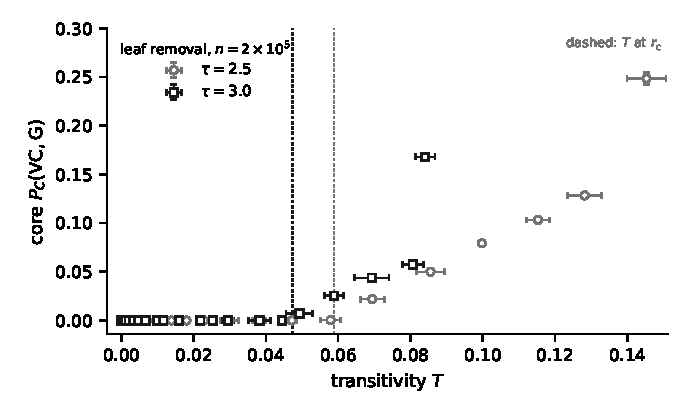
\includegraphics[width=\linewidth]{figs/fig-vw-t.pdf}
\caption{\textbf{Order parameter vs transitivity.}
Figure~\ref{fig:vw}'s measured core replotted with transitivity on the
abscissa, $T$ measured on the same graphs, and the verticals $T$ at
$r_{\mathrm{c}}$ carried across by the monotone $T(r)$. Turning $r$ makes
triangles, and the core arrives with them. It does not arrive at the same
number of them in the two tails --- $T=0.0589$ against $0.0474$, a wider spread
than the $r_{\mathrm{c}}$ it came from --- so transitivity is not the
coordinate the transition is simple in. $T$ is an outcome of $r$ and not a
control: nothing here holds it fixed. Generated by
\code{figs/\allowbreak cover.\allowbreak py:figure\_\allowbreak vw\_\allowbreak t}.}
\label{fig:vwt}
\end{figure}

\paragraph{Turning $r$ also makes triangles.} The axis is therefore not a
pure correlation axis. At $\tau=2.5$ and $n=2\times10^{5}$ the transitivity of
the drawn graphs runs from $1.6\times10^{-4}$ at $r=0$ to $0.145$ at $r=1$, and
the mechanism is starvation: a high-degree node may attach only within its own
degree class, the tail has few members to offer, and the classes saturate into
small dense blocks --- the fraction of stub pairings discarded as a repeat or a
self-loop climbs from $0$ to $0.075$ in step. So Eq.~\eqref{eq:vwr} does not
move along $e_{dd'}$ with everything else held fixed, and
Fig.~\ref{fig:vwt} is Fig.~\ref{fig:vw}'s core asked again against $T$. The
core arrives with the triangles, which is Sec.~\ref{sec:corefree}'s statement
turning up in an ensemble that was not built to make any; but it does not
arrive at the same $T$ in the two tails, $0.0589$ against $0.0474$ where
$r_{\mathrm{c}}$ was $0.7042$ against $0.7802$, a wider spread and not a
narrower one. Transitivity therefore orders the approach to the transition but
does not locate it.

This does not rescue $\{p_{d},e_{dd'}\}$, and Sec.~\ref{sec:hrg}'s reading
survives it for two reasons. The clustering arrives only at extreme
assortativity, and the hyperbolic graph and its control both sit near $r=0$,
where this ensemble's $T$ is $10^{-4}$ against the $10^{-1}$ the geometry
supplies. And it arrives on the \emph{hubs}: average local clustering, which is
Chapter~\ref{ch:data}'s $C$, rises with $r$ but vanishes as $n^{-0.4}$ at every
$r$, so almost no vertex is in a triangle even where triples are. What the
paragraph does establish is that the correlation axis carries clustering with
it, which has to be known before it is used as a null.

\paragraph{What is added here is a diagnosis, not a result.} The instability
was originally located by watching the iteration fail to converge, which is a
real signal --- the map is order-reversing, so an unstable fixed point gives a
period-two orbit and not a drift --- but it is one instrument doing two jobs,
and it cannot report a fixed point it has failed to reach. Under
Eq.~\eqref{eq:vwr} the map closes on the single scalar
$\sum_{d}q_{d}(1-\pi_{d})^{\,d}$, so nested bisection reaches the fixed point on
either side of $r_{\mathrm{c}}$ and stability is then asked of the Jacobian
there; that Jacobian is diagonal plus rank one, so its spectrum comes from a
secular equation rather than an eigensolve, and is cross-checked against one.
The algebra is in \code{vertexcover.\allowbreak py} and
Eq.~\eqref{eq:rc} is produced by
\code{statmech/\allowbreak examples/\allowbreak vw03\_\allowbreak figure1.\allowbreak py}.
The digits carry a caveat. At $\tau=3.0$ they are converged in the degree
cutoff and at $\tau=2.5$ they are not, since $\ave{k}$ itself converges slowly
against a $2.5$ tail: two decimals are real there and four at $\tau=3.0$, which
is why Eq.~\eqref{eq:rc} quotes them to different precision.

\section{Real networks}
\label{sec:realcore}
\index{leaf removal}
\index{core}

Section~\ref{sec:hrg} tested the LCZP map on an ensemble built to be
clustered. This section runs the same comparison on sixteen real
networks: the ten of Chapter~\ref{ch:data}'s
Table~\ref{tab:real} and the six Chapter~\ref{ch:overlap} works with, read from
the same cache. That chapter keeps to induced neighbourhoods of at most twenty
vertices because it enumerates $\ln Z$; leaf removal is linear, so whole
networks are used here.

The two columns are the same quantity by two routes. \emph{Leaf removal on
the graph} is the measurement, $P_{C}(\mathrm{VC},\mathrm{G})$. \emph{LCZP on
its cliques} is the prediction, $P_{C}(\mathrm{VC},\chi)$, evaluated on the
maximal-clique ensemble measured from that same graph, with nothing fitted.
What is being asked is whether the second reproduces the first --- whether
knowing a real network's degree distribution and its cliques is enough to say
how much of it leaf removal will fail on. Why the cliques should matter at all
is settled before this section and not in it: Sec.~\ref{sec:corefree} shows
algebraically that a complex of three or more members destroys the core-free
branch, and Sec.~\ref{sec:hrg} shows it on an ensemble where the clustering can
be turned against a degree-matched control. Triangles make covering hard; the
question here is how well the map counts them.

\begin{table}[t]
\centering\small
\begin{adjustbox}{max width=\linewidth}
\begin{tabular}{lrrrrr}
\hline\hline
 & & & \multicolumn{3}{c}{core fraction}\\
network & $\ave{k}$ & $C$ & leaf removal & Eq.~\eqref{eq:core} & leaf removal\\
 & & & on the graph & on its cliques & rewired\\
\hline
Euroroad & 2.51 & 0.019 & 0.1559 & 0.0162 & 0.0111\\
PDZ domains & 2.60 & 0.007 & 0.0248 & 0.0014 & 0.0000\\
Power grid & 2.67 & 0.080 & 0.0927 & 0.0337 & 0.0005\\
Yeast (Y2H) & 2.67 & 0.071 & 0.0405 & 0.0157 & 0.0000\\
C. elegans 2007 & 2.71 & 0.017 & 0.0000 & 0.0007 & 0.0000\\
C. elegans WI8 & 3.20 & 0.022 & 0.0000 & 0.0008 & 0.0000\\
Human (Stelzl) & 3.85 & 0.006 & 0.0000 & 0.0002 & 0.0002\\
Human (Vidal) & 4.32 & 0.072 & 0.0313 & 0.0056 & 0.0000\\
Co-authorship & 4.82 & 0.741 & 0.6385 & 0.7101 & 0.5983\\
Human (Figeys) & 5.79 & 0.040 & 0.0000 & 0.0010 & 0.0000\\
Les Mis. scenes & 6.60 & 0.573 & 0.5065 & 0.4731 & 0.2909\\
Football & 10.66 & 0.403 & 1.0000 & 1.0000 & 1.0000\\
Facebook & 11.88 & 0.605 & 0.8085 & 0.8444 & 0.8020\\
Collins yeast & 16.57 & 0.648 & 0.7490 & 0.7798 & 0.7129\\
Jazz bands & 27.70 & 0.617 & 0.9495 & 0.9561 & 0.9487\\
Hospital contacts & 30.37 & 0.640 & 1.0000 & 1.0000 & 1.0000\\
\hline\hline
\end{tabular}

\end{adjustbox}
\caption{\textbf{Leaf removal on sixteen real networks.} The core fraction by
two routes: $P_{C}(\mathrm{VC},\mathrm{G})$ from leaf removal run on the
graph, and $P_{C}(\mathrm{VC},\chi)$ from the LCZP map, Eq.~\eqref{eq:core}, on
that graph's own maximal-clique ensemble. $C$ is the clustering coefficient.
Ordered by mean degree, which is what sorts the rows into the three groups the
text takes them in. Generated by
\code{figs/\allowbreak cover.\allowbreak py:table\_\allowbreak real\_\allowbreak core} from
\code{statmech/\allowbreak probe/\allowbreak real\_\allowbreak core.\allowbreak py}.}
\label{tab:realcore}
\end{table}

\begin{figure}[tbp]
\centering
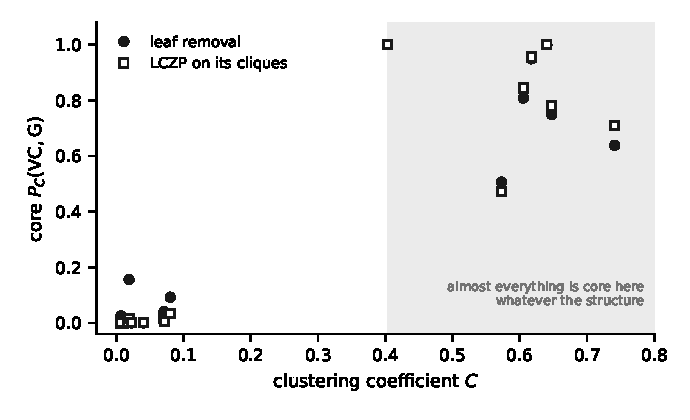
\includegraphics[width=\linewidth]{figs/fig-real-core.pdf}
\caption{\textbf{Core size against clustering for sixteen real networks.}
Table~\ref{tab:realcore}'s two core columns
against its clustering column: leaf removal on the graph, and the LCZP map on
that graph's own maximal cliques. The shading is not a third measurement. It
marks the seven networks that are already more than half core --- $0.51$ to
$1.00$, at $\ave{k}$ from $4.8$ to $30.4$ --- where returning \emph{nearly all
of it} is agreement won for free, and where the two symbols therefore sit on
top of each other. Everything the section rests on is to the left of it, and it
is compressed into the first eighth of the axis, which is the other thing the
figure is showing. Generated by
\code{figs/\allowbreak cover.\allowbreak py:figure\_\allowbreak real\_\allowbreak core}
from
\code{statmech/\allowbreak probe/\allowbreak real\_\allowbreak core.\allowbreak py}.}
\label{fig:realcore}
\end{figure}

Figure~\ref{fig:realcore} draws the table, and its shape is the warning this
section has to give before any of its numbers are read. Core rises with
clustering across the sixteen, which is the result one would like to have; but
the networks with high $C$ are also the dense ones, and a curve drawn through
the figure as a whole would be measuring $\ave{k}$. The evidence is the nine
points crowded against the ordinate, at $C\le0.08$, where the graph is sparse
enough that having a core is not automatic. The paragraphs below take the
sixteen in three groups for that reason.

\paragraph{Seven networks are already more than half core.} They run from
$0.51$ to $1.00$, at $\ave{k}$ from $4.8$ to $30.4$, and at those densities
almost every vertex is in the $2$-core before any question of clustering
arises. The chygraph tracks the measurement there --- $93$ to $111$ per cent of it
--- and that agreement establishes nothing, because a constant would have done
as well. Density is not sorted by $\ave{k}$ alone, which is why the group
is defined by the core and not by the degree: the Figeys interactome sits at
$\ave{k}=5.8$ with no core at all.

\paragraph{Five carry the comparison.} Euroroad, the PDZ and Yeast two-hybrid
interactomes, the power grid and the Vidal screen are sparse --- $\ave{k}$ from
$2.5$ to $4.3$, four of them below the Poisson threshold $\ave{k}=e$ of
Sec.~\ref{sec:onepoint} --- and all five have a core, from $0.025$ on PDZ to
$0.156$ on Euroroad. The chygraph built from their cliques predicts one on
every one of them. That threshold is a Poisson number and these degree
distributions are not Poisson, so it does not by itself say the degree
distribution could not have produced these cores; what settles that is
Sec.~\ref{sec:corefree} algebraically and Sec.~\ref{sec:hrg} on an ensemble
where the clustering can be varied at fixed degree distribution. What the five
add is that the prediction is evaluated on measured clique ensembles, with
nothing fitted, and returns a core where there is one.

\paragraph{Quantitatively it is much worse than on hyperbolic graphs.} Those
five recover $5.8$ to $38.8$ per cent of the measured core, where
Sec.~\ref{sec:hrg} recovered $77$ to $100$. The direction of the error is the
same --- the chygraph understates --- and so, presumably, is the cause, since
these are the sparsest networks in the set and Chapter~\ref{ch:data} measured
their $\mathrm{shared}_{2+}$ at $0.000$ to $0.022$: the cliques of a real
network share vertices, the map assumes they do not, and the sharing is what it
throws away. On a real network that cannot be established the way
Sec.~\ref{sec:hrg} establishes it, since the clique ensemble cannot be
rearranged with everything else held fixed. The direction is what is reported.

\paragraph{Four networks have no core at all, which is what
Sec.~\ref{sec:corefree} predicts.} The two \emph{C. elegans} screens and the
Stelzl and Figeys interactomes return exactly zero, and the LCZP map
returns between $2\times10^{-4}$ and $1\times10^{-3}$ on them. Both are right.
Section~\ref{sec:corefree} proves the core cannot vanish identically once any
complex of three or more members is present, and the paragraph that blocks the
strong reading of it says precisely this case: non-zero as the algebra requires,
and too small to see. A prediction of $10^{-4}$ on a graph of two thousand
vertices is a prediction of no core, and no core is what leaf removal finds.

\paragraph{What this adds to Sec.~\ref{sec:hrg}.} Less than the sixteen rows
suggest, and in one respect more. Eleven of the sixteen are uninformative ---
seven because almost everything is core, four because nothing is. The five that
carry the comparison agree with the hyperbolic result in direction and are
three to ten times worse in magnitude. What is new is the paragraph before
this one: the weak form of Sec.~\ref{sec:corefree}, that the core is non-zero
but can be negligible, was argued there from a constructed example with a
triangle layer of chy-degree $10^{-3}$, and here it is four real networks.

\paragraph{Three ensembles, one conclusion.} The chapter has now put the same
question to three families of graph that share no construction. Hyperbolic
graphs are clustered by the geometry they are built in, and carry a core at
every density down to $\ave{k}=0.05$ (Sec.~\ref{sec:hrg}). The correlated
graphs of Sec.~\ref{sec:vw} acquire triangles as a side effect of
assortativity, and their core appears where those triangles do. These sixteen
are clustered by whatever the data recorded, and the five sparse enough for the
question to be open have a core as well. The mechanism is the same in the three
cases and is stated in Sec.~\ref{sec:corefree}: above cardinality two the
core-free branch does not exist, so one layer of triangles is enough to remove
it. The three ensembles do not prove that --- the algebra does --- but they are
the three cases in which the prediction was made against structure the model
did not choose.

\section{Checks}
\label{sec:cover-checks}

\checkhead{Known results}
The $c=2$ threshold returns $e$ to ten digits, which is Bauer--Golinelli.
Equation~\eqref{eq:vc} at $c=2$ returns the Weigt--Hartmann cover size, agreeing
with Eq.~\eqref{eq:hs} to nine digits along a different code path.
Section~\ref{sec:vw} is a recapitulation of \citet{vazquez2003vw} and adds no
result: Eq.~\eqref{eq:vwxc} at $e_{dd'}=q_{d}q_{d'}$ and Poisson $p_{d}$
returns the Weigt--Hartmann size to machine precision at $\ave{k}=1,2,3,5,10$,
and the instability of Eq.~\eqref{eq:vwpi} at the same point returns $e$ to
fifteen digits --- a third independent route to Sec.~\ref{sec:onepoint}'s
number. The secular criterion behind Eq.~\eqref{eq:rc} and
Fig.~\ref{fig:vw} is cross-checked against a dense eigensolve of the same
Jacobian, and agrees to $8\times10^{-15}$. Figure~\ref{fig:vw}'s lower panel is
a measurement and not a recapitulation: leaf removal on graphs drawn from
Eq.~\eqref{eq:vwr} at $n=2\times10^{5}$, three seeds, brackets the onset of the
core between the grid points either side of Eq.~\eqref{eq:rc}'s
$r_{\mathrm{c}}$ at both tails, with the core zero to $4\times10^{-4}$ below
and rising steeply above. That the core and the loss of stability coincide on
the \emph{correlation} axis does not follow from Sec.~\ref{sec:onepoint}, which
establishes it on the chy-degree axis, and it is checked here rather than
assumed. The grid is $\Delta r=0.05$, so the bracket is all the resolution
claimed; no finite-size scaling of the onset was done. Figure~\ref{fig:vwt}
reparametrises that measurement and adds no data. Its abscissa is an outcome
and not a control, and it is not clean in $n$: transitivity is flat in system
size at $\tau=2.5$, drifting as $n^{-0.02}$ to $n^{-0.05}$ over a decade, but
falls as $n^{-0.15}$ at $\tau=3.0$, so at larger $n$ that curve would slide
left and the threshold spread would widen rather than close. The clustering
figures quoted with it --- $T$ against $r$, average local clustering vanishing
as $n^{-0.4}$, and the discarded-pairing fraction --- are from
\code{statmech/\allowbreak probe/\allowbreak vw\_\allowbreak clustering.\allowbreak py}
at three sizes and two seeds, which is enough for the exponents to two figures
and no more.

\checkhead{New results}
The identification of the three points, everything above cardinality two, and
the hyperbolic-graph and real-network tests are new here. On the four real
networks with no measured core, the LCZP map returns between
$2\times10^{-4}$ and $1\times10^{-3}$, which is Sec.~\ref{sec:corefree}'s weak
form --- non-zero and negligible --- met in data rather than in the constructed
example that paragraph uses. Equation~\eqref{eq:factored} is an
identity, checked symbolically; the numerical map agrees, reporting a core-free
branch at $c=2$ and none at $c=3,4,5,8$, and that the core is exactly
$1-e^{-\ave{k}}$ above cardinality two is checked against the closed form at
three cardinalities and three densities. The core-percolation threshold and the
hard-field instability of Chapter~\ref{ch:hittingset}, computed independently,
agree to $2.5\times10^{-10}$. The LCZP map is compared with pure
leaf removal on graphs built to match it, at $n=4\times10^{5}$, over eleven
ensembles at cardinalities two, three and four, with an error running from
$8.7\times10^{-5}$ to $3.1\times10^{-3}$. The multi-layer threshold
Eq.~\eqref{eq:corethresh} returns Eq.~\eqref{eq:sumkappae}'s total chy-degree
$e$ to $2\times10^{-10}$ at one, two, three and five Poisson layers, evenly and
unevenly split. Equation~\eqref{eq:vcinstab} is checked by evaluating the
instability of Eq.~\eqref{eq:vc} at its own root, which returns $1$ to ten
digits at $c=2,\dots,10$. Equation~\eqref{eq:smallcore} agrees with the
numerical map to $10^{-4}$ relative or better at $c=3,4,5,8$ and three link
densities, and reproduces the $1.8\times10^{-4}$ of
Sec.~\ref{sec:corefree}'s constructed example. Table~\ref{tab:five} recomputes
nothing: each row is Eq.~\eqref{eq:vc} and Eq.~\eqref{eq:core} on one list of
cardinalities, and its three cardinality-two rows agree with each other, and its
hypergraph rows with the closed form $1-\Phi(0)$, to every digit printed.

\checkhead{Partial results}
Section~\ref{sec:realcore} establishes less than sixteen rows suggest, and the
text says which rows carry it. Seven of the networks are already more than half
core, so a prediction of nearly all of it agrees for free; four have no core at
all. Five carry it, and on those the chygraph recovers $5.8$ to $38.8$ per cent
of the measured core against Sec.~\ref{sec:hrg}'s $77$ to $100$ --- the same
direction, three to ten times worse. The overlap that
Sec.~\ref{sec:hrg} identifies as the cause by rearranging its ensemble cannot
be isolated that way on a real network, so the direction is reported and the
attribution is carried over rather than remeasured.
Section~\ref{sec:vw}'s digits are not all converged: at $\tau=2.5$ the
degree cutoff still moves $r_{\mathrm{c}}$ and $x_{c}$ in the third decimal,
because $\ave{k}$ itself converges slowly against that tail, so two decimals
are quoted there against four at $\tau=3.0$. None of the structural claims ---
the ordering of the two curves, monotonicity in $r$, replica symmetry at $r=0$
--- depends on that, and the published figure has not been digitised, so the
agreement with it is structural and not numerical.
Figure~\ref{fig:hrgc} recomputes no core: it is
\code{prediction4}'s columns joined to the clustering of the same graphs,
measured on regenerated copies at the same seeds and calibration, and its
abscissa is produced by $\ave{k}$ rather than varied against it. Transitivity
was measured first and rejected: on these tails it is flat in $\ave{k}$ and
separated by seed --- $0.009$ to $0.011$ against $0.016$ to $0.021$ at
$\tau=2.5$ --- because a few hubs of degree $10^{3}$ own its denominator, and
the rejection is recorded here because the same coordinate does work in
Sec.~\ref{sec:vw}, where the degrees are bounded by the cutoff and the
triangles are on the hubs by construction.
Section~\ref{sec:hrg} establishes less than its numbers suggest, and both
qualifications are carried in the text. The
\emph{existence} of the core follows from the algebra the moment a single
triangle enters the ensemble, so it was never at risk. Only the exponent could
have failed, and there the predicted value does not move with the tail while the
measured one does: they agree within errors at $\tau=2.5$ and differ at
$\tau=2.9$ by roughly four standard deviations. What lies past $\ave{k}=e$ --- the
complexity, and the one-step answer for this family --- is not computed here.


% sources
% - the retired manuscript, Sec. VI and supplement Sec. VI
% - ../probe/prediction4.py (hyperbolic random graphs)

\chapter{Colouring}
\label{ch:colouring}
\index{graph colouring|textbf}

This chapter and the next complete Part~III's third family. Chapter~\ref{ch:hittingset}
minimised a set subject to a covering constraint; Chapter~\ref{ch:cover}
tightened the constraint and found the algorithm that solves it. Colouring
keeps the hard constraint and drops the minimisation: there is nothing to
optimise, only a question of whether a configuration exists at all.

It is also the place where a promise made in Chapter~\ref{ch:potts} comes due.
Proper colouring is the antiferromagnetic $q$-state Potts model at zero
temperature --- this book's own model at the opposite sign --- so if the
machinery is what it has been claimed to be, the colouring calculation should be
a substitution and not a new theory. It is, and the substitution produces two
closed forms.

One is a surprise. For proper colouring, the transmission of a complex does not
depend on its cardinality at all: a clique of nine members transmits exactly what
a single edge does. The other is the opposite: for the weaker hypergraph
constraint the transmission collapses like $q^{-c}$, and by cardinality four a
complex has almost stopped constraining anything. Identical at cardinality two,
these two problems diverge violently above it, and
Sec.~\ref{sec:twoconstraints-col} is why.

\section{Colouring as a hard-core problem}
\label{sec:colouringdef}

Give every node one of $q$ colours and forbid an edge whose endpoints agree.
There is no chemical potential and no ground-state energy to minimise: a
colouring either exists or it does not, and the question is at what density of
constraints it stops existing.

In the language of Chapter~\ref{ch:statmech} this is
Eq.~\eqref{eq:emitted} with an interior that assigns weight zero to forbidden
configurations and weight one to the rest. Nothing else changes. What does
change, before any algebra, is the \emph{message}. Up to now a message has been one number --- a probability, a field, an integer, or
at worst three states. Here it is a distribution over $q$ colours,
$\eta_{i\to a}(\sigma)$, and there is no ferromagnetic direction to project it
onto. That is the sense in which colouring is heavier than anything before it,
and Sec.~\ref{sec:colouring-scalar} is the observation that rescues it.

\paragraph{Two constraints, not one.} On a graph there is only one way to
forbid, but on a chygraph a complex of $c$ members admits two natural rules and
they are not the same.

\emph{Proper colouring} of the induced graph: every pair inside a complex is an
edge, so all $c$ members must take \emph{distinct} colours. This needs $q\ge c$
and is what one means by colouring a clustered graph whose motifs have been
promoted to complexes.

\emph{Hypergraph colouring}: only a \emph{monochromatic} complex is forbidden.
Two members may agree as long as not all of them do. This is the standard
higher-order generalisation, and it is strictly weaker.

At $c=2$ the two coincide, which is exactly why the distinction has no
counterpart on a graph. Above it they are different problems, and
Chapter~\ref{ch:cover}'s pairing of hitting set with vertex cover was the same
distinction one family earlier: how much of a complex may be left alone.

\section{What a complex transmits}
\label{sec:colouring-scalar}
\index{transmission factor}

The uniform assignment $\eta\equiv1/q$ is always a fixed point --- every colour
equally likely everywhere, which is the replica-symmetric solution. Linearise
about it and one number governs the result.

\begin{calculation}{one number, because the colours are interchangeable}
Write $\eta_{j}=1/q+w_{j}$ with $\sum_{\sigma}w_{j}(\sigma)=0$, which is forced
because both $\eta$ and $1/q$ are normalised. The perturbations therefore live
in the $(q-1)$-dimensional traceless subspace, and permuting the colours is a
symmetry of the whole problem. By Schur's lemma the linearised map acts on that
subspace as a \emph{scalar}. So although the message carries $q-1$ numbers, its
linearisation carries one, and Chapter~\ref{ch:statmech}'s branching matrix
applies unchanged with that scalar in place of $u'$. This is checked directly:
three different traceless directions return one number.

\emph{Proper colouring.} The emitted quantity is
\[
  Z(\sigma_{0})=\!\!\sum_{\substack{\sigma_{1}\dots\sigma_{c-1}\ \text{distinct}\\
    \text{and all}\ \ne\sigma_{0}}}\ \prod_{j}\eta_{j}(\sigma_{j}).
\]
Differentiate with respect to $\eta_{1}(s)$. The result is zero unless
$s\ne\sigma_{0}$, and when $s\ne\sigma_{0}$ it is the same quantity $A$ for
every such $s$, because the remaining sum depends only on how many colours have
been excluded and not on which. So the linear response is
\[
  \sum_{s}w_{1}(s)\,A\,\mathbf{1}[s\ne\sigma_{0}]
  =A\Bigl(\sum_{s}w_{1}(s)-w_{1}(\sigma_{0})\Bigr)=-A\,w_{1}(\sigma_{0}),
\]
the first sum vanishing by tracelessness. With
$A=q^{2-c}(q-2)!/(q-c)!$ and $Z_{0}=q^{1-c}(q-1)!/(q-c)!$ at the uniform point,
the ratio $A/Z_{0}=q/(q-1)$, and after normalising,
\begin{equation}
  \tau_{c}(q)=-\frac{1}{q-1}.
  \label{eq:taucol}
\end{equation}
Every combinatorial factor cancels. The cardinality has gone.

\emph{Hypergraph colouring.} Here the constraint removes a single configuration,
so
\[
  Z(\sigma_{0})=1-\prod_{j}\eta_{j}(\sigma_{0}),
\]
and expanding the product to first order gives, after the same normalisation,
\begin{equation}
  \tau^{\mathrm{hyp}}_{c}(q)=-\frac{1}{q^{\,c-1}-1}.
  \label{eq:tauhyp}
\end{equation}
At $c=2$ this is Eq.~\eqref{eq:taucol}, as it must be.
\end{calculation}

Both forms are confirmed by enumerating the interior exactly, in rational
arithmetic, so the agreement is an identity rather than a numerical
coincidence.

Figure~\ref{fig:colouring} draws both, and the contrast is the chapter in one
picture: three cardinalities lying exactly on top of one another for the proper
rule, and fanning out over three decades for the hypergraph one.

\paragraph{Why the cardinality cancels, in words.} What one member
of a clique learns from another is a single fact: \emph{not that colour}. It
learns the same fact from every other member. Because the perturbation is
traceless --- the colours have to keep summing to one --- excluding one colour
is the whole of the information, and excluding it again from a second member
adds nothing to the linear response. A clique of nine transmits what an edge
transmits.

The negative sign is not decoration either. Colouring is an
\emph{antiferromagnet}: raising the probability of a colour at one node lowers
it at the next. Chapter~\ref{ch:statmech} warned that the sign of the entries,
not of the leading eigenvalue, is what classifies a map, and this is the third
map in the book whose entries are negative --- after the hard-field maps of
Chapters~\ref{ch:hittingset} and~\ref{ch:cover}.

\begin{figure}[t]
\centering
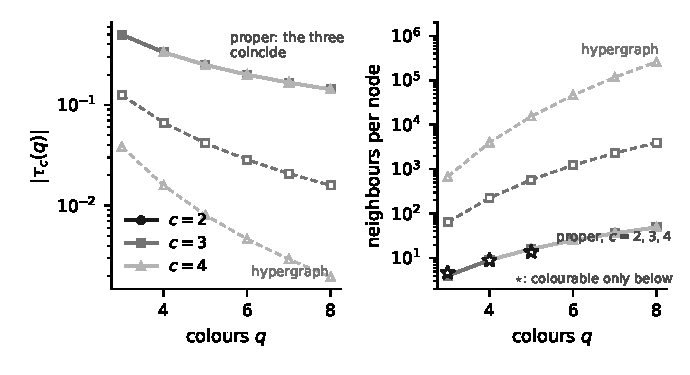
\includegraphics[width=\linewidth]{figs/fig-colouring.pdf}
\caption{\textbf{Two constraints, identical at cardinality two.} Left: the
transmission of a complex, Eqs.~\eqref{eq:taucol} and~\eqref{eq:tauhyp}. For
proper colouring (solid) the three cardinalities fall exactly on top of one
another, each curve starting at $q=c$ since a smaller palette admits no proper
colouring at all; for hypergraph colouring (dashed) the transmission collapses
like $q^{-c}$. Right: the resulting local-stability threshold in neighbours per
node. Proper colouring sits at $(q-1)^{2}$ whatever the cardinality --- the
graph value; hypergraph colouring runs away as $(q^{c-1}-1)^{2}$. Stars are the
published colourability thresholds for Erd\H{o}s--R\'enyi graphs
\citep{mulet2002}, which lie \emph{below} the stability line for $q\ge4$: see
Sec.~\ref{sec:colouring-rsb}. Generated by \code{figs/colouring.py}.}
\label{fig:colouring}
\end{figure}

\section{The threshold, and what it is}
\label{sec:colouringthreshold}
\index{de Almeida--Thouless line}

Substituting into Eq.~\eqref{eq:branch} needs one decision, and it is the
decision Chapter~\ref{ch:ising} already made in Sec.~\ref{sec:atline}.

There is no ordered phase to look for here: the uniform solution \emph{is} the
replica-symmetric solution, and what one asks is whether a perturbation of
\emph{random sign} grows. That perturbation is transmitted with $\tau$ and its
effect measured by squaring, so the operative condition is the de
Almeida--Thouless form --- $\ave{u'}$ replaced by $\ave{u'^{2}}$ everywhere,
which by Eq.~\eqref{eq:reweight} is an elementwise reweighting and nothing more.
For a single layer,
\begin{equation}
  \ave{\kbar}\,(c-1)\,\tau_{c}^{2}=1.
  \label{eq:colthresh}
\end{equation}

\paragraph{The graph case, against the literature.} Put $c=2$, where a complex
is an edge and the chy-degree is the ordinary degree. What is left to choose is
the degree distribution. For a \emph{Poisson} one, $\ave{\kbar}=\ave{k}$ ---
a Poisson distribution being its own excess --- and Eq.~\eqref{eq:colthresh}
gives $\ave{k}=(q-1)^{2}$. For a \emph{regular} one, a node of degree $k$ has
$k-1$ other edges, so $\ave{\kbar}=\ave{k}-1$ and it gives
$\ave{k}=(q-1)^{2}+1$. Both are
Ref.~\citep{zdeborova2007}'s Eq.~(18), which reads
$c_{\mathrm{RS}}^{\mathrm{ER}}=q^{2}-2q+1$ and
$c_{\mathrm{RS}}^{\mathrm{reg}}=q^{2}-2q+2$; the stability analysis and its
large-$q$ asymptotics are worked out in Ref.~\citep{krzakala2004}, and the
replica treatment of the same ensemble in Ref.~\citep{vanmourik2002}.

Two published expressions from one $\tau$, and the difference between them is
exactly the excess-degree convention this book has been carrying since
Sec.~\ref{sec:map}. That is the check the chapter needed, and it is a stronger
one than a single number would have been, because a formalism that had the
excess bookkeeping wrong would reproduce at most one of the two lines.

\paragraph{Cardinality, and the two constraints.} Now raise it. Counting in
\emph{neighbours} per node --- a complex of cardinality $c$ supplies $c-1$ of
them --- Eq.~\eqref{eq:colthresh} gives
\begin{equation}
  \text{proper: } (q-1)^{2},
  \qquad
  \text{hypergraph: } \bigl(q^{\,c-1}-1\bigr)^{2}.
  \label{eq:coltwo}
\end{equation}
The first does not move. A network of $c$-cliques loses stability at exactly the
same number of neighbours per node as a graph does, for every cardinality and
every $q$: promoting motifs to complexes changes nothing at all here. The second
runs away --- at $q=4$ it is $9$, $225$, $3969$ for $c=2,3,4$.

The second is not new, and the agreement is a check rather than a result.
Reference~\citep{gabrie2017} solves $q$-colouring of $K$-uniform random
hypergraphs and its Eq.~(43) gives the same linear-stability bound,
$\ell^{\mathrm{RS}}_{\mathrm{stab}}=(q^{K-1}-1)^{2}/(K-1)$ for a Poisson degree
of mean $\ell$ --- which is $(q^{c-1}-1)^{2}$ neighbours per node, this
chapter's Eq.~\eqref{eq:coltwo}. Its Appendix~B derives the transmission at
finite temperature and Eq.~\eqref{eq:tauhyp} is that expression at
$\beta\to\infty$. What is left to this chapter is the first line and the
contrast: that the same substitution gives both rules, and that they part
company only above cardinality two.

The first of these is the same phenomenon as Eq.~\eqref{eq:kc}, which found
$\ave{k}(c-1)=e$ for hitting set: counted in neighbours, hyperedge size does not
move the point. Two hard-core problems, two different constants, one structure.
The reason is the same both times --- what a complex transmits and how many
neighbours it supplies move in exactly compensating ways. This is the
\emph{opposite} of the Ising model, where Sec.~\ref{sec:clustering} found the two effects failing to compensate and
the multiplicity winning.

\section{The two constraints diverge above cardinality two}
\label{sec:twoconstraints-col}

Equation~\eqref{eq:coltwo} says the following.

Proper colouring of a clique network is, at this level of description,
indistinguishable from colouring a graph with the same number of neighbours.
Hypergraph colouring of the same object is not remotely the same problem: a
cardinality-four complex over four colours tolerates $3969$ neighbours per node
where the proper constraint tolerates $9$.

The gap is entirely a matter of how much a complex forbids. A clique of four
rules out all but $q(q-1)(q-2)(q-3)$ of $q^{4}$ assignments; the monochromatic
rule leaves all but $q$ of them. At $c=2$ those are the same statement and the
distinction is invisible --- which is why it has no name in the graph
literature, and why it needed a formalism with cardinality in it to become
visible.

This is the third time Part~III has found a distinction that exists only above
cardinality two. Section~\ref{sec:hardfail} found the hard-field limit exact at
$c=2$ and wrong above it; Sec.~\ref{sec:corefree} found the core-free branch
present at $c=2$ and absent above it; and here two constraints coincide at $c=2$
and separate by three orders of magnitude above it. The pattern is not a
coincidence. Cardinality two is degenerate in a specific way --- a complex with
two members has no room for a partial violation --- and a great deal of what
looks like general theory is an artefact of working there.

\section{A graph with triangles}
\label{sec:colouring-triangles}

Cardinality independence has a consequence the previous section did not draw,
and it is the one case where the chapter's constraint and the book's running
comparison meet.

For \emph{proper} colouring a triangle-clustered graph is not a new object at
all. A triangle forbids its three members from agreeing pairwise, which is what
its three edges already say, so the problem is ordinary $q$-colouring of an
ordinary graph and the graph calculation applies to it. Put a regular network in
which every vertex sits in $\kappa$ triangles, so that its degree is $n=2\kappa$
and the triangles meet only at vertices. Then Eq.~\eqref{eq:colthresh} on the
chygraph of triangles gives $\ave{\kbar}(c-1)=2(\kappa-1)=n-2$, while the same
network read as a graph of degree $n$ gives $\ave{\bar k}=n-1$. The two answers
are
\begin{equation}
  \text{chygraph: } n=(q-1)^{2}+2,
  \qquad
  \text{graph: } n=(q-1)^{2}+1,
  \label{eq:tridisagree}
\end{equation}
and they disagree by one in degree at every $q$.

The chygraph is the right one, for the reason the book has been giving since
Sec.~\ref{sec:treelike}. The graph calculation adds the messages arriving at a
vertex as though its neighbours were independent; inside a triangle two
neighbours are adjacent, and the three edges close a loop. Promoting the
triangle to a complex puts that loop inside Eq.~\eqref{eq:emitted}, where it is
summed exactly, and leaves a structure over triangles that really is treelike.
The graph answer is not an approximation that happens to be close --- it is off
by exactly the one branch the loop costs.

\paragraph{Both ends of one formula.} Nothing above required dropping a layer.
Take links and triangles together at fixed degree, with $a$ the link chy-degree,
$b$ the triangle chy-degree, $n=a+2b$, and $f=2b/n$ the fraction of degree
carried by triangles. Because $\tau$ does not depend on cardinality, both layers
carry the same $s=\tau^{2}=(q-1)^{-2}$, and the two-layer determinant of
Eq.~\eqref{eq:LT} reads
\begin{equation}
  s\,(n-3)+2s^{2}\bigl[n(1-f/2)-1\bigr]=1 .
  \label{eq:trifamily}
\end{equation}
At $f=0$ this returns $(q-1)^{2}+1$ and at $f=1$ it returns $(q-1)^{2}+2$,
exactly and in rational arithmetic, with the cross term doing all of the
interpolating. The two lines of Eq.~\eqref{eq:tridisagree} are one formula at
its two ends.

\paragraph{How big is it, honestly.} One in degree, and only for regular
ensembles. For Poisson layers $\ave{\kbar}=\ave{\kappa}$, the cross term
$\ave{\kappa}_{|}\ave{\kappa}_{\triangle}-\ave{\kbar}_{|}\ave{\kbar}_{\triangle}$
vanishes identically, and Eq.~\eqref{eq:trifamily} returns $(q-1)^{2}$ at every
$f$: there is no difference at all. So this is not a statement that clustering
moves the colouring threshold. It is the regular ensemble's lost branch, the
same one that separates $(q-1)^{2}$ from $(q-1)^{2}+1$ in
Sec.~\ref{sec:colouringthreshold}, arriving where it can be mistaken for
physics. Chapter~\ref{ch:ising} found clustering worth $13.9$ per cent in
$T_{c}$ and Sec.~\ref{sec:helporhurt} found it worth a fifth of $q_{c}$; here it
is worth one in degree, and for half the ensembles nothing.

That is the third sign the book has taken on this comparison, and the least
dramatic of them. It is included because the cheap conclusion --- that a
formalism built for higher-order structure must find higher-order structure
mattering --- is wrong, and the arithmetic that shows it is wrong is three
lines.

\section{Where replica symmetry goes}
\label{sec:colouring-rsb}
\index{replica symmetry breaking}

Now the qualification, and it is a large one. Colouring is the classic
one-step replica-symmetry-breaking problem, and Eq.~\eqref{eq:colthresh} is not
a one-step answer. So it is important to say precisely what it is and, more
importantly, what it is not; Sec.~\ref{sec:colouring-sp} then does the
calculation it is not.

It is the point where the replica-symmetric solution loses \emph{local}
stability --- where the spin-glass susceptibility diverges. It is not the
colourability threshold. Comparing with the published Erd\H{o}s--R\'enyi values
\citep{mulet2002} gives Table~\ref{tab:colpublished}.
\begin{table}[t]
\centering\small
\begin{tabular}{rrrr}
\hline\hline
$q$ & $(q-1)^{2}$ & clustering $c_{d}$ & colourable to $c_{q}$\\
\hline
$3$ & $4$ & $4.42$ & $4.69$\\
$4$ & $9$ & $8.27$ & $8.90$\\
$5$ & $16$ & $12.67$ & $13.69$\\
\hline\hline
\end{tabular}
\caption{\textbf{A local stability line is not a colourability line.} Eq.~\eqref{eq:colthresh} at cardinality two against the published Erd\H{o}s--R\'enyi clustering and colourability thresholds \citep{mulet2002}. At $q=3$ the instability sits inside the colourable phase; from $q=4$ upward it sits above the colourability threshold, so it is on the wrong side rather than merely loose.}
\label{tab:colpublished}
\end{table}

At $q=3$ the local instability sits inside the colourable phase, below both the clustering
transition and the colourability threshold. At $q=4$ and above it sits
\emph{above} the colourability threshold --- the graph has long since stopped
being colourable by the time the replica-symmetric solution notices anything is
wrong. The criterion is not merely loose there; it is on the wrong side.

That is not a defect of the chygraph construction. It is the known behaviour of
replica-symmetric colouring, and Ref.~\citep{zdeborova2007} records it in the
same words: the instability threshold lies in the colourable phase only for
$q=3$. What this chapter contributes is that the same statement, with the same
constants, comes out of the general branching matrix; and that it extends to
complexes, where Eq.~\eqref{eq:coltwo} says a clique network behaves exactly like
a graph and a hypergraph does not.

\paragraph{What is needed instead.} The colourability threshold requires the
one-step calculation --- survey propagation and the iterative algorithms built
on it \citep{braunstein2003,mulet2002}, and a complexity function. The next
section does that much. What it does not do is the condensation and rigidity
transitions Ref.~\citep{zdeborova2007} maps out, or the rigorous side of the
same question \citep{cojaoghlan2016}.

Whatever it returns, Eq.~\eqref{eq:coltwo} remains a statement about the
stability of a particular solution and not about when colourings run out --- and
the interesting part of it, that cardinality drops out of the proper constraint
and dominates the hypergraph one, is a statement about the interior sum that a
one-step treatment inherits unchanged, because Eqs.~\eqref{eq:taucol}
and~\eqref{eq:tauhyp} are properties of a complex and not of an ansatz.

\section{Surveys, and colourability}
\label{sec:colouring-sp}
\index{survey propagation|textbf}
\index{replica symmetry breaking}

Table~\ref{tab:colpublished} has three columns and the chapter has so far
produced one of them. This section produces the other two, and it produces them
by redoing a published calculation rather than by extending one. Survey
propagation for colouring is Refs.~\citep{braunstein2003,mulet2002}', the
thresholds it returns are theirs, and nothing below is a new result. It is here
because a book that spends a chapter saying its own threshold is the wrong line
should be able to compute the right one, and because the machinery is then in
place for cardinalities above two, where Sec.~\ref{sec:colouring-sp-chy} takes
it.

The object one level up is a survey: a distribution, over the clusters of
colourings, of the colour a node is forced to. Colour symmetry does most of the
work of carrying it. A survey is uniform over colours, so one scalar per
inclusion suffices --- $e$, the probability that a node is forced at all, with
each colour taking $e/q$ of it.

What symmetry does \emph{not} do is decouple the colours, and this is the whole
of the calculation. A forced neighbour forbids exactly one colour, so ``every
colour but one is forbidden'' is a question about whether $q-1$ colours are
\emph{covered} by the forced neighbours, not a product of $q-1$ independent
events. Inclusion--exclusion over which colours are missed gives
\begin{equation}
  \begin{split}
    P(\text{only }c\text{ free})&=\sum_{j=0}^{q-1}(-1)^{j}\binom{q-1}{j}
      \prod_{k}\Bigl(1-\frac{e_{k}(1+j)}{q}\Bigr),\\
    P(\text{none free})&=\sum_{j=0}^{q}(-1)^{j}\binom{q}{j}
      \prod_{k}\Bigl(1-\frac{e_{k}j}{q}\Bigr),
  \end{split}
  \label{eq:colsp}
\end{equation}
the product running over the other neighbours, and the survey update being the
first divided by one minus the second --- the contradictory state discarded, as
in Sec.~\ref{sec:sat-sp}. Treating the colours as independent instead is the
obvious shortcut and it is wrong; it is caught by asking for three thresholds
rather than one.

The complexity is Eq.~\eqref{eq:sigma} with one term fewer, a graph having no
complexes above cardinality two to sum over:
\begin{equation}
  \Sigma=\bigl\langle\ln\bigl(1-P(\text{none free})\bigr)\bigr\rangle
        -\frac{\ave{k}}{2}\Bigl\langle\ln\Bigl(1-\frac{e_{i}e_{j}}{q}\Bigr)
        \Bigr\rangle,
  \label{eq:colsigma}
\end{equation}
the edge term being the weight of two ends not forced to the same colour.

\begin{table}[t]
\centering\small
\begin{tabular}{rccr}
\hline\hline
$q$ & $\Sigma=0$ at & $c_{q}$ published & error\\
\hline
$3$ & $4.683\,(0.012)$ & $4.69$ & $-0.1\%$\\
$4$ & $8.901\,(0.012)$ & $8.90$ & $+0.0\%$\\
$5$ & $13.660\,(0.008)$ & $13.69$ & $-0.2\%$\\
\hline\hline
\end{tabular}
\caption{\textbf{The colourability threshold, computed.} Where the complexity of
Eq.~\eqref{eq:colsigma} vanishes, against Mulet's $c_{q}$
\citep{mulet2002}. Bracketed figures are the spread over three seeds. Compare
the $(q-1)^{2}$ column of Table~\ref{tab:colpublished}: $4$, $9$ and $16$ against
these. Generated by \code{figs/colouring.py}.}
\label{tab:colsp}
\end{table}

Table~\ref{tab:colsp} is the result. Set beside Table~\ref{tab:colpublished} it
says what Sec.~\ref{sec:colouringthreshold} could not: at $q=4$ the stability
line sits at $9$ and the colourings run out at $8.90$, so the replica-symmetric
solution is still locally stable after the problem has become unsolvable, and
the size of that error is now a number rather than a direction.

The clustering threshold arrives without further work, though less sharply. The
density at which the surveys stop being trivial --- below which no cluster
forces anything and $e$ collapses to zero --- is $c_{d}$, and it comes out of
the same population that gives $\Sigma$: $4.46$ against a published $4.42$ at
$q=3$, and $8.49$ against $8.27$ at $q=4$. That is a per cent and then three,
against a tenth of a per cent for $c_{q}$, and the asymmetry is the expected
one. A vanishing complexity is a crossing and can be bisected; a branch
appearing is a fold, and a population of twenty thousand locates it less well.
Both remaining columns of Table~\ref{tab:colpublished} nonetheless come from one
calculation, with neither used in getting there.

\paragraph{The same three qualifications.} They are
Sec.~\ref{sec:sat-sp}'s and they apply here unchanged: this is $m=0$, so the
condensation and rigidity transitions are outside it; the treelike condition of
Eq.~\eqref{eq:up} is untouched; and reproducing published constants is a check
on the implementation, not a result. To say it once more, since a section that
computes five-figure agreement can be mistaken for one that discovers
something: every number in Table~\ref{tab:colsp} was already known. What the
chygraph adds is that Eqs.~\eqref{eq:colsp} and~\eqref{eq:colsigma} are written
for an arbitrary chy-degree distribution and an arbitrary interior, which is
what makes the next section a substitution rather than a second derivation.

\section{Above cardinality two, and what the rule costs}
\label{sec:colouring-sp-chy}
\index{survey propagation}

The previous section stayed at $c=2$, where the chygraph is a graph and the
answer was already known. This section raises the cardinality, and the interest
is not in the numbers --- those are known too --- but in which of the two rules
survives the step and which does not.

\paragraph{What a complex has to tell a member.} In the hard-field limit the
message from a complex is the set of colours it forbids the member it is
speaking to. Everything about how that message combines with the others at a
node turns on one question: \emph{how many colours can a single complex forbid
at once?}

For the hypergraph rule the answer is \textbf{at most one}. A complex is
violated only when all of its members share a colour, so it can forbid $\gamma$
to member $0$ only when every one of the other $c-1$ members is already forced
to $\gamma$ --- and they cannot all be forced to two different colours at the
same time. The message is therefore the same \emph{kind} of object as at
cardinality two, a single forbidden colour or none, and Eq.~\eqref{eq:colsp}
carries over with one substitution: the weight $e/q$ that a neighbour forbids a
given colour becomes $h/q$, where
\begin{equation}
  h=q\prod_{j=1}^{c-1}\frac{e_{j}}{q}
  \label{eq:hypsp}
\end{equation}
is the weight that the complex forbids anything at all. Nothing else in the
node update changes, and the inclusion--exclusion of
Sec.~\ref{sec:colouring-sp} is reused unaltered.

For the proper rule the answer is \textbf{up to $c-1$}. Every member forced to a
different colour removes a different colour from member $0$, so a complex of
cardinality five can arrive carrying four prohibitions at once. The message is
no longer a colour but a \emph{set} of them, the events ``$\gamma$ is
forbidden'' and ``$\gamma'$ is forbidden'' are correlated within a single
complex as well as across complexes, and the node update needs the joint
distribution of the forbidden set rather than a scalar. Equation~\eqref{eq:colsp}
does not carry over, and no substitution repairs it.

That asymmetry is Sec.~\ref{sec:twoconstraints-col} again, one level up. There
the two rules were found to coincide at cardinality two and to separate above
it, in what they transmit. Here they coincide at cardinality two and separate
above it in something harder: whether the one-step machinery can be reused at
all. A complex with two members has no room for a partial violation, and it also
has no room to forbid two things at once; both statements are the same
degeneracy, and it is the second that decides how much work the next calculation
is.

\paragraph{Carrying it out.} Put Eq.~\eqref{eq:hypsp} into
Eq.~\eqref{eq:colsp}. The complexity of Eq.~\eqref{eq:colsigma} gains the one
term a graph does not have: a complex is violated when all $c$ of its members
agree, so it contributes
$\ln\bigl[1-q\prod_{j\le c}(e_{j}/q)\bigr]$, and there are
$\ave{k}/c$ complexes per node.

\begin{table}[t]
\centering\small
\begin{tabular}{ccccr}
\hline\hline
$q$ & $c$ & $\Sigma=0$ at & published & error\\
\hline
$3$ & $3$ & $26.900\,(0.000)$ & $26.92$ & $-0.07\%$\\
$4$ & $3$ & $63.276\,(0.024)$ & $63.30$ & $-0.04\%$\\
$2$ & $5$ & $52.283\,(0.043)$ & $52.32$ & $-0.07\%$\\
\hline\hline
\end{tabular}
\caption{\textbf{Hypergraph colouring above cardinality two.} Mean chy-degree at
which the complexity vanishes, against the colourability thresholds of
Ref.~\citep{gabrie2017}, Table~1. Bracketed figures are the spread over three
seeds. The three errors agree in sign and size, which is a converged bias of the
finite population rather than scatter. Generated by \code{figs/colouring.py}.}
\label{tab:hypsp}
\end{table}

Table~\ref{tab:hypsp} is the result.

The three rows are Ref.~\citep{gabrie2017}'s colourability thresholds, and the
agreement is a check on the substitution and not a new result: that paper solves
this problem, and Sec.~\ref{sec:colouringthreshold}'s hypergraph threshold is
its Eq.~(43). What the check establishes is that Eq.~\eqref{eq:hypsp} is the
whole of the difference --- that once a complex can forbid at most one colour,
cardinality enters the one-step calculation through a single scalar and through
nothing else.

\paragraph{Two exclusions, both real.} At $q=2$ with $c=3$ and $c=4$
Ref.~\citep{gabrie2017} marks its colourability threshold as invalid, the $m=0$
solution being unstable to noise propagation there. The calculation above will
return a number for those cases and it would mean nothing; they are omitted from
the table for that reason and not because they disagree. And the proper rule is
absent from the table because of the paragraph above, not because it was tried
and failed: a set-valued survey is a different calculation, and this book does
not do it.

\section{Checks}
\label{sec:colouring-checks}

\emph{Against enumeration, exactly.} Equations~\eqref{eq:taucol}
and~\eqref{eq:tauhyp} are checked against a direct enumeration of the interior
of a complex, in rational arithmetic so that the agreement is exact rather than
numerical: proper colouring for $q=3,\dots,7$ at every cardinality from $2$ to
$\min(q,5)$, and hypergraph colouring for $q=3,4,5$ at cardinalities $2$, $3$
and $4$.

\emph{That one number suffices.} The claim that the linearised map acts as a
scalar on the traceless subspace is checked by perturbing along three different
traceless directions and requiring the same answer, for both rules.

\emph{Against the literature.} Equation~\eqref{eq:colthresh} at $c=2$ returns
$(q-1)^{2}$ for a Poisson degree distribution and $(q-1)^{2}+1$ for a regular
one, which are the two lines of Ref.~\citep{zdeborova2007}'s Eq.~(18). The published thresholds of
Ref.~\citep{mulet2002} are quoted alongside, and the chapter states that they
lie below the stability line for $q\ge4$ rather than leaving that to be
discovered.

\emph{What is not checked, because it is not claimed.} Nothing here is a
colourability threshold. This chapter computes where a replica-symmetric
solution stops being locally stable, and Sec.~\ref{sec:colouring-rsb} is the
account of the difference.


% sources
% - no manuscript: the calculations are done in figs/colouring.py
% - benchmarks: Mulet et al. PRL 89, 268701 (2002), Table I (ER thresholds);
%   Zdeborova & Krzakala PRE 76, 031131 (2007), Eq. (18) (RS local stability,
%   c = (q-1)^2 for ER and (q-1)^2 + 1 for regular)
% - references under ~/Downloads/chygraph_references/

\chapter{Satisfiability}
\label{ch:satisfiability}

Satisfiability is the fourth hard-core family and the last technical chapter of
Part~III. It is also the one where the book's machinery is furthest from
sufficient, and saying exactly how far is most of what this chapter does.

The mapping is the easiest in the book: variables are atoms, clauses are
complexes, and a clause forbids exactly one assignment of its members. That is
Chapter~\ref{ch:colouring}'s hypergraph rule with one forbidden configuration
instead of two. But one feature does not carry over, and it decides everything.
Colouring's constraint is symmetric under permuting the colours, so the uniform
message is a fixed point and the threshold has a closed form.
A clause is not symmetric: it forbids a \emph{particular} assignment, the one
its signs pick out. The uniform message is not a fixed point, the disorder has
to be carried, and no closed form survives.

What does survive is a hard-field treatment --- Chapter~\ref{ch:hittingset}'s
warning propagation, on this chygraph --- and it produces one exact result, one
structural statement, and one honest failure. The exact result is the $2$-SAT
threshold. The structural statement is that for $k\ge3$ the trivial fixed point
is stable at \emph{every} clause density, so there is no linear instability at
all. The failure is that the hard field then goes on reporting nothing wrong
well past the point where the formula has stopped being satisfiable.

\section{Clauses as complexes}
\label{sec:clauses}

A $k$-SAT formula over $N$ Boolean variables is a conjunction of $M$ clauses,
each a disjunction of $k$ literals --- a variable or its negation. A clause is
satisfied unless every one of its literals is false, so each clause forbids
exactly one of the $2^{k}$ assignments of its variables. The control parameter
is the clause density $\alpha=M/N$.

The chygraph is immediate. Layer $0$ is the variables, as atoms; layer $1$ is
the clauses, as complexes of cardinality $k$. A variable's chy-degree is the
number of clauses it appears in, so for a random formula it is Poisson with mean
$\ave{\kappa}=k\alpha$: each clause holds $k$ variable slots and there are
$\alpha N$ clauses.

\paragraph{The one thing that is new.} Every complex in this book so far has
carried an interaction that treats its members alike. A clause does not. It
carries $k$ \emph{signs}, and the assignment it forbids depends on them. Two
clauses on the same $k$ variables can forbid different assignments, and in a
random formula they do.

That is quenched disorder living \emph{inside} a complex, and it is the first
time the book has met any. Chapter~\ref{ch:statmech} allowed it without
comment --- Eq.~\eqref{eq:emitted} takes $-\beta H$ as an argument and does not
ask whether it is the same for every complex --- but the consequence is real,
and Sec.~\ref{sec:whatclausetransmits} is it.

\section{What a clause transmits}
\label{sec:whatclausetransmits}

Write $u_{j}$ for the value of variable $j$ that falsifies its literal in clause
$a$. Then the interior sum of Eq.~\eqref{eq:emitted} removes a single
configuration, and
\begin{equation}
  Z_{a\to0}(\sigma_{0})
    =1-\mathbf{1}[\sigma_{0}=u_{0}]\prod_{j\in a\setminus0}\eta_{j}(u_{j}).
  \label{eq:satZ}
\end{equation}
Compare Eq.~\eqref{eq:tauhyp}'s parent, $Z=1-\prod_{j}\eta_{j}(\sigma_{0})$: the
same shape, with the product taken at a fixed assignment rather than along the
diagonal. Satisfiability really is colouring at $q=2$ with the symmetry broken,
and Eq.~\eqref{eq:satZ} is where the breaking enters.

The consequence is worth seeing before any analysis. Put every incoming message
at $\eta=1/2$. Then Eq.~\eqref{eq:satZ} emits $1-2^{1-k}$ on the falsifying
value and $1$ on the other: at $k=3$, $3/4$ against $1$. The emitted message is
\emph{not} uniform, so the uniform message is not a fixed point.

That single fact separates this chapter from the last one. In
Chapter~\ref{ch:colouring} the colour-permutation symmetry gave a uniform fixed
point, Schur's lemma reduced the linearised map to one number, and
Eq.~\eqref{eq:taucol} followed in three lines. Here the symmetry is broken
clause by clause. It is restored only \emph{on average} over the signs, which
means the object that has a symmetric fixed point is the distribution of
messages and not a message. There is no scalar to linearise, and no closed form
of the kind Eq.~\eqref{eq:taucol} provides.

\section{Warning propagation}
\label{sec:sat-wp}

What is available is the hard-field limit, which is Chapter~\ref{ch:hittingset}
transplanted. Keep only whether a message is a \emph{warning}: clause $a$ warns
variable $i$ that $i$ must satisfy $a$, because every other member of $a$ has
already been forced to falsify it.

\begin{calculation}{the warning map, and the factor of one half}
Let $\eta$ be the probability that a clause sends a warning along an inclusion,
and $\pi$ the probability that a variable reached along one is forced to a given
value.

\emph{Down.} A clause warns $i$ only when all $k-1$ other members are forced to
falsify it, so
\[
  \eta=\pi^{\,k-1}.
\]

\emph{Up.} A variable is forced by the warnings arriving from its \emph{other}
clauses. Here the signs enter, and they enter once: a warning arriving at $j$
points at one of the two values, and the chance that it is the value falsifying
the clause under consideration is $1/2$. So with $\bar\Phi$ the excess
chy-degree generating function, the mean number of warnings arriving in the
relevant direction is $\ave{\kbar}\eta/2$, and for Poisson chy-degree
\[
  \pi=\bigl(1-e^{-\ave{\kbar}\eta/2}\bigr)\,e^{-\ave{\kbar}\eta/2},
\]
the two factors being ``at least one warning that way'' and ``none the other
way''. A variable receiving warnings both ways is a contradiction, not a
forcing. Putting the two steps together with $\ave{\kbar}=k\alpha$,
\begin{equation}
  \eta=\Bigl[\bigl(1-e^{-k\alpha\eta/2}\bigr)e^{-k\alpha\eta/2}\Bigr]^{k-1}.
  \label{eq:wp}
\end{equation}
\end{calculation}

Equation~\eqref{eq:wp} is Chapter~\ref{ch:hittingset}'s
Eq.~\eqref{eq:hs} with two changes, and both are worth naming.

The first is the factor $1/2$, and it is the whole of what negatable variables
buy. A hyperedge in Chapter~\ref{ch:hittingset} constrains its members in one
way only; a clause can constrain them either way, so half the warnings a
variable receives are irrelevant to any given clause.

The second is a sign. Chapter~\ref{ch:hittingset}'s map was
order-\emph{reversing}, which is why it needed the $F\circ F$ bracket of
Sec.~\ref{sec:hard} and why plain iteration oscillated. Equation~\eqref{eq:wp}
is order-\emph{preserving}: more warnings force more variables, which send more
warnings. Monotone iteration from zero suffices, exactly as for
Chapter~\ref{ch:cover}'s leaf removal. The two hard-field problems in this book
sit on opposite sides of the sign test that Sec.~\ref{sec:fixedpoint} said would
decide which solver applies, and here is the second of them.

\section{Two-SAT is exact; above it there is no threshold at all}
\label{sec:twosat}

Now linearise Eq.~\eqref{eq:wp} at $\eta=0$. Since $\pi\simeq k\alpha\eta/2$ for
small $\eta$,
\begin{equation}
  \frac{\partial\eta'}{\partial\eta}\bigg|_{0}
    =\lim_{\eta\to0}\Bigl(\frac{k\alpha\eta}{2}\Bigr)^{k-1}\Big/\eta
    =\begin{cases}
       \alpha, & k=2,\\[2pt]
       0, & k\ge3.
     \end{cases}
  \label{eq:satslope}
\end{equation}

\paragraph{$k=2$.} The trivial fixed point loses stability at
\begin{equation}
  \alpha=1,
\end{equation}
and the non-trivial branch grows continuously out of it --- $\eta^{*}=0$ at
$\alpha=0.99$ and $0.0066$ at $\alpha=1.01$. That is the exact $2$-SAT
threshold, which is one of the few thresholds in this subject known rigorously.
It comes out of the general branching condition with no adjustment, and it is
the chapter's benchmark.

\paragraph{$k\ge3$.} The derivative is not small; it is \emph{zero}, at every
clause density. A clause needs $k-1$ warnings at once before it will emit one,
so a single warning cannot start anything, and $\eta\equiv0$ is stable however
many clauses one adds.

This is Sec.~\ref{sec:groupcontagion}'s exclusion, in its purest form. There a
group needed $r\ge2$ infected members and a single seed could not invade; here a
clause needs $k-1$ forced variables and a single warning cannot propagate. The
book has now met the same structure four times --- interdependent networks,
threshold contagion, the Potts model above $q=2$, and satisfiability above
$k=2$ --- and this is the extreme case, because there is no linear instability
anywhere on the axis to mistake for a transition.

The non-trivial branch arrives instead by a fold (Fig.~\ref{fig:sat}). At $k=3$
the map first touches the diagonal at $\alpha=5.39$; below that the only
solution is $\eta=0$.

\begin{figure}[t]
\centering
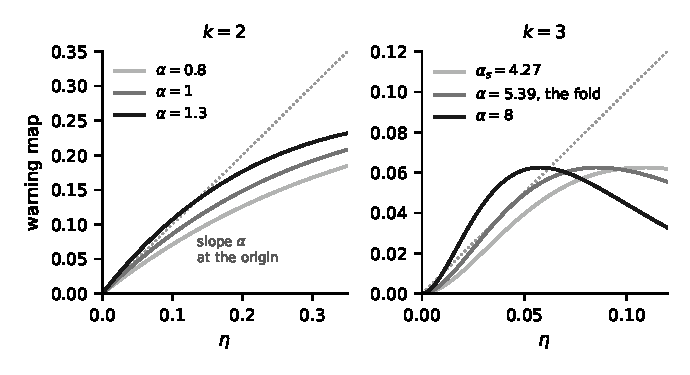
\includegraphics[width=\linewidth]{figs/fig-sat.pdf}
\caption{\textbf{Why two is different.} The warning map,
Eq.~\eqref{eq:wp}, against the diagonal. Left, $k=2$: the map leaves the origin
with slope $\alpha$, so it crosses the diagonal as soon as $\alpha>1$ and the
branch grows continuously. Right, $k=3$: it leaves the origin with slope zero
whatever $\alpha$, so the origin is a fixed point at every density and the
branch can only arrive by a tangency --- here at $\alpha=5.39$, which is well
past the density $\alpha_{s}=4.27$ at which the formula has stopped being
satisfiable. Generated by \code{figs/satisfiability.py}.}
\label{fig:sat}
\end{figure}

\section{Where the hard field is blind}
\label{sec:satblind}

The fold is not the satisfiability threshold, and the gap is the point of this
section.

\begin{center}\small
\begin{tabular}{rrrr}
\hline\hline
$k$ & warning fold & $\alpha_{s}$ & ratio\\
\hline
$2$ & $1.000$ & $1$ & $1.00$\\
$3$ & $5.386$ & $4.267$ & $1.26$\\
$4$ & $18.24$ & $9.931$ & $1.84$\\
$5$ & $61.58$ & $21.12$ & $2.92$\\
\hline\hline
\end{tabular}
\end{center}

The published thresholds are from Ref.~\citep{montanari2008}. Read the last
column: the warning map first notices that something is wrong at a density
$1.26$ times the true one at $k=3$, and nearly three times it at $k=5$. Below
its fold, warning propagation reports no warnings, no contradictions and no
difficulty --- for formulas that are, with probability approaching one,
unsatisfiable.

That is the same defect as Sec.~\ref{sec:hardfail}, one family later and one
degree worse. There, collapsing the field onto an integer discarded an $O(1)$
part and returned a cover of one half where the answer was one third. Here it
discards the same kind of information and the answer is not merely wrong but
uninformative over a wide range of densities.

\paragraph{How much of that number to believe.} Less than the table's digits
suggest, and the chapter had better say which parts are solid.

The two results of Sec.~\ref{sec:twosat} are linearisations, so they do not
depend on how a variable receiving contradictory warnings is counted. The fold
does. Under the strict convention used above --- contradictory warnings are a
contradiction, not a forcing --- the $k=3$ fold is $5.386$; counting instead the
\emph{net} warning field, so that opposing warnings partly cancel, it is
$4.667$. The numbers move by fifteen per cent and more.

What does not move is the direction. Under either convention the fold lies above
$\alpha_{s}$ at every $k$ tried: $4.667$ against $4.267$ at $k=3$, $11.83$
against $9.93$ at $k=4$, $27.91$ against $21.12$ at $k=5$. So the qualitative
statement is robust and the number is a bookkeeping choice, and the table above
should be read as the first and not the second.

\section{Where replica symmetry goes}
\label{sec:sat-rsb}

Random $k$-SAT is the problem for which one-step replica symmetry breaking was
invented, and the reason is visible in the gap just measured.

The correct object is not a single warning probability but a \emph{distribution}
over warnings --- a survey --- and propagating it is survey propagation
\citep{mezard2002science,mezard2002pre}. That calculation returns
$\alpha_{s}=4.267$ for $k=3$, and the intermediate structure that this chapter
cannot see: a clustering transition at $\alpha_{d}=3.86$ where the solutions
shatter into exponentially many groups, and for $k\ge4$ a condensation
transition between the two \citep{montanari2008}.

So the position here is the same as in Chapter~\ref{ch:colouring} but more
acute. There, the replica-symmetric calculation gave a definite closed form that
was a local stability threshold rather than a colourability one. Here even that
is unavailable, because there is no symmetric fixed point to linearise about,
and the hard-field substitute is blind over a range that grows with $k$.

\paragraph{What the chygraph adds, and what it does not.} It adds the structure:
Eq.~\eqref{eq:wp} is written for an arbitrary chy-degree distribution, mixed
clause lengths are one layer per length, and correlations between a variable's
participation in short and long clauses are Sec.~\ref{sec:joint}'s joint
$\Phi$ --- none of which a fixed-$k$, Poisson treatment reaches. It does not add
the one-step calculation, and for this problem that is where the subject
begins rather than ends.

The honest summary is that satisfiability is the model in this book that most
needs what this book does not do. It is included because the mapping is exact
and instructive, because $2$-SAT comes out right, and because the way it fails
is the same way Chapter~\ref{ch:hittingset} failed --- which is worth knowing
about a method one intends to apply elsewhere.

\section{Checks}
\label{sec:sat-checks}

\emph{Against enumeration.} Equation~\eqref{eq:satZ} is checked against a direct
enumeration of a clause's $2^{k}$ assignments for $k=2,3,4$, in rational
arithmetic, including the emitted values at $\eta=1/2$ that establish the
absence of a uniform fixed point.

\emph{Against a rigorous result.} Equation~\eqref{eq:satslope} at $k=2$ gives
$\alpha=1$, the exact $2$-SAT threshold, and the non-trivial branch is confirmed
to be absent at $\alpha=0.99$ and present at $\alpha=1.01$.

\emph{That the derivative really vanishes.} For $k\ge3$ the claim is that a
derivative is zero, which a single finite difference cannot establish. What is
checked is the \emph{rate}: the finite difference at $\varepsilon$ falls like
$\varepsilon^{k-2}$, verified by halving $\varepsilon$ and requiring the ratio
$2^{k-2}$, at $k=3,\dots,6$ and three clause densities each.

\emph{Against the convention.} Both conventions for a contradicted variable are
run. They agree at $k=2$, where the answer is a linearisation, and disagree
above it; both put the fold above $\alpha_{s}$. The chapter quotes the
disagreement rather than one convention's numbers alone.

\emph{What is not checked, because it is not claimed.} Nothing here is a
satisfiability threshold except at $k=2$. Section~\ref{sec:satblind} is the
account of the difference, and Sec.~\ref{sec:sat-rsb} of what would close it.


% sources
% - no manuscript. Mezard, Parisi & Zecchina Science 297, 812 (2002);
%   Mezard & Zecchina PRE 66, 056126 (2002); Montanari, Ricci-Tersenghi &
%   Semerjian (2008); Franz & Leone (2003)
% - references under ~/Downloads/chygraph_references/

\part{Limits}

\chapter{When complexes overlap}
\label{ch:overlap}

This is the chapter the whole book has been deferring to, and it is the honest
one.

Every calculation in Parts~II and~III rests on one assumption, stated in
Sec.~\ref{sec:treelike} and repeated whenever it mattered: complexes meet in at
most one node. Chapter~\ref{ch:statmech} located it precisely, in the step where
a node adds what its complexes have told it as though they were independent.
The assumption is what buys the whole apparatus, and on the networks
Chapter~\ref{ch:data} measured, it is false.

So this chapter asks three questions in order. How much does the violation
cost? What would repair it? And why is the repair not simply the next chapter of
this book rather than an open problem? The answers are: less than one might
fear but not nothing; a region graph with messages on it; and because the repair
is known at the level of one network and not at the level of an ensemble, which
is the level everything else here works at.

\section{The price of treelikeness}
\label{sec:price}

Chapter~\ref{ch:chygraphs} sold the central move as follows. A triangle is a
loop, and a loop is what a tree-based calculation cannot have; promote the
triangle to a complex, sum over its interior exactly, and the loop is gone from
the outside view.

That move is real and Chapter~\ref{ch:ising} measured what it buys. But it does
not remove loops. It moves them up one level. Two triangles sharing an
\emph{edge} are a loop in the incidence structure --- a cycle through complex,
node, complex, node --- exactly as a triangle is a loop in a graph. The chygraph
cannot see it, for the same reason and by the same argument
(Fig.~\ref{fig:sharededge}).

\begin{figure}[t]
\centering
\begin{adjustbox}{max width=\linewidth}
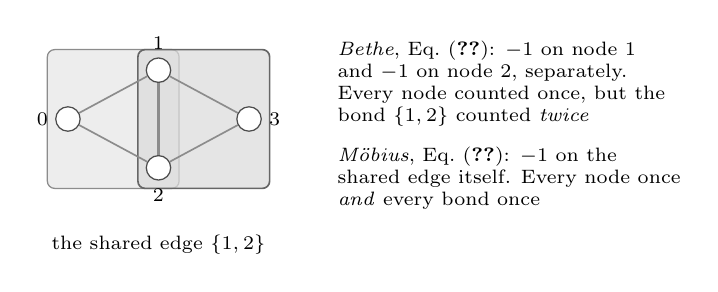
\begin{tikzpicture}
% Two triangles sharing the edge {1,2}: a loop one level up.
\node[nd] (v0) at (-1.15,0) {};
\node[nd] (v1) at (0,0.62) {};
\node[nd] (v2) at (0,-0.62) {};
\node[nd] (v3) at (1.15,0) {};
\node[lb,anchor=east] at (-1.28,0) {$0$};
\node[lb,anchor=south] at (0,0.76) {$1$};
\node[lb,anchor=north] at (0,-0.76) {$2$};
\node[lb,anchor=west] at (1.28,0) {$3$};
\draw[lnk] (v0)--(v1) (v0)--(v2) (v1)--(v2) (v1)--(v3) (v2)--(v3);
\draw[lnk,line width=1.3pt] (v1)--(v2);
\begin{scope}[on background layer]
  \node[cx,fit=(v0)(v1)(v2)] {};
  \node[cxb,fill opacity=0.72,fit=(v1)(v2)(v3)] {};
\end{scope}
\node[lb,anchor=north,align=center] at (0,-1.35)
  {the shared edge $\{1,2\}$};
% the two countings
\node[lb,anchor=west,align=left] at (2.15,0.45)
  {\emph{Bethe}, Eq.~\eqref{eq:bethe}: $-1$ on node $1$\\
   and $-1$ on node $2$, separately.\\
   Every node counted once, but the\\
   bond $\{1,2\}$ counted \emph{twice}};
\node[lb,anchor=west,align=left] at (2.15,-0.75)
  {\emph{M\"obius}, Eq.~\eqref{eq:mobius}: $-1$ on the\\
   shared edge itself. Every node once\\
   \emph{and} every bond once};
\end{tikzpicture}
\end{adjustbox}
\caption{\textbf{A loop one level up.} Two triangles sharing an edge. Promoting
each triangle to a complex removes its internal loop from the outside view, but
the two complexes now meet in two nodes rather than one, and the cycle
complex--node--complex--node is invisible to a chygraph exactly as a triangle is
invisible to a graph. Both counting schemes count every node once; only one also
counts the shared bond once, and that is the difference between subtracting a
correlation and not.}
\label{fig:sharededge}
\end{figure}

The correct statement is therefore not that chygraphs solve clustering. It is
that they move the boundary of what counts as local, from ``no loops'' to ``no
loops \emph{between} complexes''. That is a real gain --- Chapter~\ref{ch:cover}
measured it on hyperbolic random graphs, where the degree-matched control has no
core at all and the chygraph has very nearly the right one --- and it is not the
same as a solution.

\section{Measuring the deficit}
\label{sec:deficit}

How much is left on the table can be measured, and Chapter~\ref{ch:cover}
already did most of it. On hyperbolic random graphs with maximal cliques as
complexes, the chygraph accounts for $77$ to $100$ per cent of the leaf-removal
core, with the shortfall tracking the clique overlap: negligible in a sparse
graph, where cliques rarely share edges; irrelevant once almost everything is
core; worst in between.

The sharp measurement is the \emph{rewired control} of
Sec.~\ref{sec:hrg}, and it deserves restating here because it is what licenses
the rest of this chapter. Take the measured clique ensemble and rearrange it so
that complexes meet in at most one node, holding the ensemble fixed and changing
only the arrangement. The prediction agrees with that control to $10^{-3}$. So
the map is right on its own terms, and the entire remaining discrepancy against
the real graph is overlap and nothing else. Without that control one could not
tell a wrong recursion from a violated assumption; with it, the diagnosis is
unambiguous.

\paragraph{A prior question: does the ensemble exist?} Taking maximal cliques as
complexes presumes the clique-size distribution has a limit --- specifically that
the excess cardinality $\ave{\sbar}=\ave{c^{2}}/\ave{c}-1$ of
Eq.~\eqref{eq:sbaru} converges. It is worth checking rather than assuming, and
the check separates two things.

Measured against a degree-matched control at identical degree sequence and seed,
so that $P(k)$ and assortativity are held fixed and clustering is the only
difference, the paired ratio $\ave{\sbar}_{\mathrm{HRG}}
/\ave{\sbar}_{\mathrm{control}}$ is a converged constant between $1.8$ and $4.8$
for $\tau\ge2.5$, flat over $n=10^{3}$ to $3\times10^{5}$. The clustering signal
is a multiplicative factor, not a finite-size artefact. At $\tau=2.1$ both
diverge and the control diverges \emph{faster}, so the ratio decays toward one
and nothing measured there separates clustering from the tail. That is why
Sec.~\ref{sec:hrg}'s $\tau=2.1$ row behaved differently from the others, and it
is a caution rather than a result: below $\tau=2.5$ the measured ensemble is not
converged, and neither is anything built on it.

\section{Region graphs}
\label{sec:regions}

The repair is not new physics. It is the next level of the same idea, and it has
been available since Kikuchi.

Belief propagation is exact on a tree because a tree can be decomposed into
nodes and edges with each variable counted once. When it is not a tree, the
remedy is to work with larger \emph{regions} --- sets of variables treated as
units --- and to choose counting numbers so that every variable, and every
interaction, is still counted once.

Close the complex family under intersection and assign counting numbers by
M\"obius inversion:
\begin{equation}
  c_{R}=1-\sum_{R'\supsetneq R}c_{R'}.
  \label{eq:mobius}
\end{equation}

Two things follow immediately, and the first is the reassuring one.

\emph{It contains what the book has been doing.} When complexes meet in at most
one node, the family closes on the complexes plus the single nodes, and
Eq.~\eqref{eq:mobius} gives $c_{v}=1-k$ --- precisely the counting of
Eq.~\eqref{eq:bethe}. Chapter~\ref{ch:statmech}'s free energy was a region-graph
free energy all along, on the region graph a treelike chygraph happens to have.
That is why Sec.~\ref{sec:freeenergy} could say its weights were not chosen.

\emph{It departs from it exactly where complexes overlap.} On two triangles
sharing an edge, M\"obius inversion puts $-1$ on the shared \emph{edge};
Eq.~\eqref{eq:bethe} puts $-1$ on each of its two endpoints. Both count every
node once. Only one counts the shared \emph{bond} once: summing the counting
numbers of every region containing $\{1,2\}$ gives $1$ under
Eq.~\eqref{eq:mobius} and $2$ under Eq.~\eqref{eq:bethe}. The Bethe scheme
subtracts the two shared vertices independently and so never removes the
correlation between them.

That is not a subtlety to be taken on trust. The example has four spins and can
be settled by enumeration.

\section{Two triangles, exactly}
\label{sec:twotriangles}

Couple every pair inside each triangle, evaluate $\ln Z$ exactly by summing over
all sixteen configurations, and compare.

\begin{center}\small
\begin{tabular}{rrrrr}
\hline\hline
$\beta J$ & exact & Bethe & M\"obius & GBP\\
\hline
$0.2$ & $2.8887$ & $+1.8\times10^{-2}$ & $-1.4\times10^{-3}$ & $-4\times10^{-14}$\\
$0.5$ & $3.5907$ & $+9.1\times10^{-2}$ & $-2.9\times10^{-2}$ & $-2\times10^{-13}$\\
$1.0$ & $5.7390$ & $+3.7\times10^{-1}$ & $-6.6\times10^{-2}$ & $-3\times10^{-14}$\\
$2.0$ & $10.6938$ & $+1.3$ & $-1.7\times10^{-2}$ & $-5\times10^{-15}$\\
\hline\hline
\end{tabular}
\end{center}

Three readings, in increasing order of interest.

The correction is a factor of three to eighty, so the counting matters and is
not a formality. The two schemes err in \emph{opposite} directions:
Eq.~\eqref{eq:bethe} overestimates $\ln Z$ because it never removes the
correlation between the shared vertices, and Eq.~\eqref{eq:mobius} removes it
and slightly overshoots.

And the overshoot is not a property of the counting. It is a property of
evaluating a counting on \emph{isolated} regions, which is an estimate and not a
fixed point. Running the messages removes it entirely. The last column is
generalised belief propagation in its parent-to-child form \citep{yedidia2005},
iterated to a fixed point on the region graph of Eq.~\eqref{eq:mobius}, and the
error is at the level of double precision at every coupling.

\begin{calculation}{the update that is being run}
A message lives on a directed edge of the region graph, from a region $P$ to a
direct child $R$, and is a function of the child's variables. Write
$U_{R}=\{R\}\cup\mathrm{descendants}(R)$, and $f_{R}$ for the product of every
factor whose scope lies inside $R$. The belief on a region collects every
message entering $U_{R}$ from outside it,
\[
  b_{R}(x_{R})\ \propto\ f_{R}(x_{R})
    \!\!\prod_{(I\to J):\ J\in U_{R},\ I\notin U_{R}}\!\! m_{I\to J}(x_{J}),
\]
and imposing the consistency condition $\sum_{x_{P}\setminus x_{R}}b_{P}=b_{R}$
cancels every message common to the two sides. What is left is the update:
\begin{equation}
  m_{P\to R}(x_{R})=
  \frac{\displaystyle\sum_{x_{P}\setminus x_{R}}f_{P\setminus R}(x_{P})
        \prod_{N(P,R)}m}
       {\displaystyle\prod_{D(P,R)\setminus(P,R)}m},
  \label{eq:p2c}
\end{equation}
with
\[
  \begin{aligned}
    N(P,R)&=\{(I,J):J\in U_{P}\setminus U_{R},\ I\notin U_{P}\},\\
    D(P,R)&=\{(I,J):J\in U_{R},\ I\in U_{P}\setminus U_{R}\}.
  \end{aligned}
\]
The two index sets look forbidding and are doing something simple: $N$ collects
what flows into the part of $P$ that is not $R$, and $D$ divides out what has
already been counted on the way down.

The check that this is the right generalisation is what it degenerates to. On
the two-layer region graph of a pairwise model --- one region per interaction
plus one per variable --- $D(P,R)$ holds only the edge being updated, $N(P,R)$
is the set of incoming messages to the interaction's other variables, and
Eq.~\eqref{eq:p2c} \emph{is} ordinary belief propagation. So generalised belief
propagation contains belief propagation exactly as Eq.~\eqref{eq:mobius}
contains Eq.~\eqref{eq:bethe}, and Sec.~\ref{sec:overlap-checks} reports the
numerical form of that statement.
\end{calculation}

\begin{calculation}{why it is exact here, and what that does not prove}
The region family closes on $\{0,1,2\}$, $\{1,2,3\}$ and $\{1,2\}$ once the
zero-counting singletons are dropped, and that is a junction tree: a tree of
regions in which the intersection of any two regions is contained in every
region on the path between them. Generalised belief propagation on a junction
tree is exact, for the same reason belief propagation on a tree is.

So the whole of what the table reports as left on the table is recoverable ---
but by an argument that says exactly when it is recoverable, which is when the
closed complex family is a junction tree. For maximal cliques that means the
graph is chordal, and a hyperbolic random graph is not.

One more thing this calculation settles. Generalised belief propagation refuses
to run on a region graph whose counting numbers do not cover every factor once,
and the Bethe counting on two overlapping triangles is exactly such a graph. The
failure is detected rather than silently absorbed, which is worth having: the
scheme knows the shape of its own assumption.
\end{calculation}

\section{Sixty instances, and where it stops}
\label{sec:sixty}

One example proves a possibility, not a method. Figure~\ref{fig:gbp} runs the
three schemes over sixty maximal-clique region graphs of hyperbolic random
graphs --- $n=14$, $18$ and $20$, small enough to enumerate exactly, at two
couplings, keeping only the instances that are not already treelike.

\begin{figure}[t]
\centering
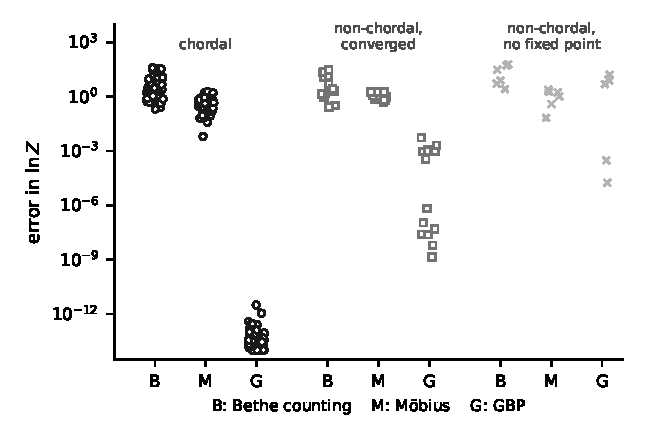
\includegraphics[width=\linewidth]{figs/fig-gbp.pdf}
\caption{\textbf{What the messages buy, and where they stop buying it.} Error in
$\ln Z$ for sixty maximal-clique region graphs of hyperbolic random graphs,
under the Bethe counting (B), the M\"obius counting evaluated on isolated
regions (M), and generalised belief propagation run to a fixed point (G).
Where the clique structure is chordal the region graph is a junction tree and
GBP is exact. Where it is not, GBP still gains two to nine orders of magnitude
--- when it converges. On six of the twenty non-chordal instances it does not
converge at all, even at damping $0.999$, and there it buys nothing. Data from
\code{probe/gbp\_cliques.py}; plotted by \code{figs/overlap.py}.}
\label{fig:gbp}
\end{figure}

The forty chordal instances come out exact, the worst error being
$3\times10^{-12}$. That is the previous section's argument holding at scale
rather than on one hand-picked example.

The twenty non-chordal instances divide, and the division is the point of this
chapter. Fourteen converge, and there the GBP error runs from
$1.4\times10^{-9}$ to $5.4\times10^{-3}$, against $0.48$ to $1.8$ for the
M\"obius counting and $0.26$ to $30$ for the Bethe counting on the same
instances --- two to nine orders of magnitude better, with the consistency
condition $\sum_{x_{P}\setminus x_{R}}b_{P}=b_{R}$ satisfied to
$2\times10^{-6}$, so what remains is the approximation's error and not the
solver's.

The other six do not converge, at any damping tried up to $0.999$. Their
residual says so, and no number from them is quoted. It is that instability,
rather than the accuracy where it converges, that matters for what comes next.

\paragraph{Two further limits, stated because the calculation is easy to
over-read.} Generalised belief propagation is not variationally bounded, so on a
region graph built from complexes that contain one another it can be
\emph{worse} than the static estimate --- covering $K_{4}$ by its four triangles
rather than by $K_{4}$ itself gives an error of $10^{-2}$ against a static
$4\times10^{-3}$. That case does not arise for maximal cliques, which never
nest, but it is a reason not to build region graphs carelessly.

And it is an \emph{instance-level} calculation. It takes an explicit list of
complexes and an explicit interaction. Everything else in this book works at the
level of an ensemble, where a message is a distribution over a chy-degree class
rather than a function on one region.

\section{Merging the offenders}
\label{sec:merging}

There is a repair more direct than a region graph, and it is worth working out
because it is the first thing anyone proposes on seeing
Fig.~\ref{fig:sharededge}: if two complexes share more than one atom, stop
treating them as two. Merge them into a single \emph{meta-complex} holding the
union of their atoms, and sum its interior exactly.

Nothing has to be added to the formalism to do this. A complex whose vertices
are complexes is what a chygraph \emph{is} --- it is the freedom
Chapter~\ref{ch:satisfiability} used to nest clauses --- and
Eq.~\eqref{eq:emitted} does not care how large or how internally tangled a
complex is, only that its interior can be enumerated. On
Fig.~\ref{fig:sharededge}'s example the merge is immediate: the two triangles
become one complex of four atoms, its $2^{4}=16$ interior states are summed
exactly, and the overlap is gone because there is nothing left for it to overlap
with. Section~\ref{sec:twotriangles}'s whole discrepancy disappears, and by a
route that needs no region graph and no parent-to-child update.

So the question is not whether the repair is correct. It is what it costs.

\paragraph{Merging is a percolation problem.} The cost is $2^{c}$ on the merged
complex, so everything turns on how large the merging grows. And that is a
question this book already has the machinery for.

Put a node on every complex, and a link between two complexes that share two or
more atoms. The meta-complexes are the connected components of that graph. The
repair is affordable exactly while that graph has \emph{no giant component} ---
and the moment it has one, the merging swallows a finite fraction of the network
into a single complex whose interior cannot be enumerated at any price.

Two details make the closure slightly more than one pass of connected
components. Merging is iterated: two meta-complexes assembled from disjoint
components can still share two atoms between their \emph{unions}, so the
procedure must be run to a fixed point. And the merged complex inherits every
inclusion of its parts, so its chy-degree is the sum --- which is what makes the
component grow.

\paragraph{What it costs on the ensemble this book is about.} Measured on
hyperbolic random graphs with maximal cliques as complexes, the answer is
discouraging and precise (Fig.~\ref{fig:merge}).

\begin{center}\small
\begin{tabular}{rrrrr}
\hline\hline
$\ave{k}$ & $n=1000$ & $n=2000$ & $n=4000$ & largest meta-complex\\
\hline
$0.3$ & $4.7$ & $5.3$ & $5.3$ & bounded\\
$0.5$ & $6.0$ & $12.3$ & $14.7$ & grows\\
$0.8$ & $19.0$ & $54.0$ & $67.0$ & grows\\
$1.5$ & $40.3$ & $208.7$ & $175.7$ & grows\\
$3.0$ & $289.7$ & $655.3$ & $1102.3$ & grows\\
\hline\hline
\end{tabular}
\end{center}

Below $\ave{k}\simeq0.4$ the largest meta-complex is a handful of atoms and does
not move with $n$: the merging terminates, the repair is exact, and it is
cheap. Above it the largest meta-complex grows with the network, reaching
twenty-eight per cent of all vertices at $\ave{k}=3$ and sixty-six per cent at
$\ave{k}=6$. At that point $2^{c}$ has an extensive exponent, which is the
original problem returned in a different costume.

\begin{figure}[t]
\centering
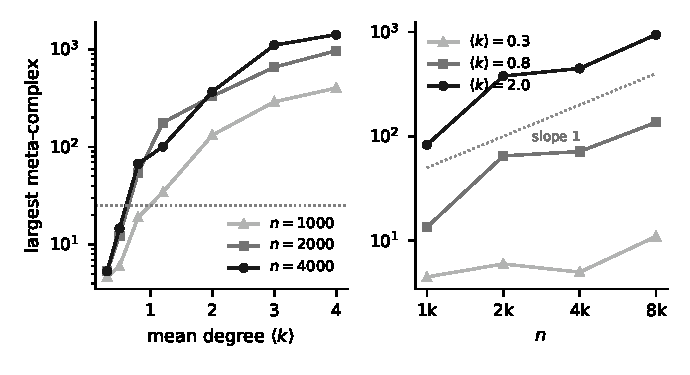
\includegraphics[width=\linewidth]{figs/fig-merge.pdf}
\caption{\textbf{When merging is affordable.} Largest meta-complex after
merging every pair of maximal cliques that share two or more atoms, iterated to
a fixed point, on hyperbolic random graphs at $\tau=2.5$. Left: against mean
degree, at three sizes; the dotted line is $2^{25}$ states, a fair limit for
exact enumeration. Right: against $n$, with a slope-one guide. At
$\ave{k}=0.3$ the largest meta-complex does not grow and the repair is exact
and cheap; by $\ave{k}=2$ it is a fixed fraction of the network. Generated by
\code{figs/merge.py}.}
\label{fig:merge}
\end{figure}

\paragraph{What to take from this.} Three things, and the first is not a
disappointment.

The repair is \emph{right}, and it is right for the reason the whole book is
organised around: a complex is allowed to contain complexes, so absorbing an
overlap into a bigger interior is a legal move rather than a patch. Where it
terminates, it gives the exact answer with no approximation anywhere and no
region graph to build.

The threshold that decides it is a percolation threshold on the overlap graph,
which is the sort of object Chapter~\ref{ch:percolation} computes. So the
feasibility of the Part~IV repair is a Part~II calculation --- one can ask, of a
given ensemble, whether merging will terminate, before attempting it. That is a
better position than discovering it by running out of memory.

And on the ensembles that motivated the construction it terminates only in the
very sparse régime. This is not special to hyperbolic graphs: clustering is
exactly what makes cliques share edges, so any ensemble with enough clustering
to need the repair tends to have enough to make it percolate. The two conditions
pull against each other, which is why Sec.~\ref{sec:whatwouldclose}'s route ---
messages between regions, rather than one enormous region --- remains the one
that scales. Merging and generalised belief propagation are the two ends of one
dial: merge everything and the messages become trivial but the interior
impossible; merge nothing and the interior is easy but the messages
approximate. Where to sit on that dial is an ensemble-by-ensemble question, and
Fig.~\ref{fig:merge} is how one answers it.

\paragraph{A practical note.} Between those extremes lies a range where merging
is worth doing on the instances one actually has, rather than on an ensemble.
Finding which complexes to merge is a mechanical, checkable operation: build the
overlap graph, take components, verify no two survivors share two atoms, verify
each is small enough to enumerate. It is exactly the kind of bookkeeping that is
tedious by hand, easy to get subtly wrong, and well suited to being automated.
A tool that took a network, proposed a merge closure, and reported the largest
interior it produced would tell a user in one pass whether the exact route is
open to them --- and the answer would be a number rather than a judgement.

\section{Clustering is a hierarchy of obstructions}
\label{sec:hierarchy}

Step back and the shape of the difficulty is visible.

A graph cannot see a triangle. Promote triangles to complexes and the chygraph
cannot see two triangles sharing an edge. Promote \emph{those} pairs to regions
and the region graph cannot see whatever loops the regions form among
themselves. Each level removes the obstruction below it and exposes the one
above. This is not a defect of the construction; it is what the cluster
variation method has always been, and the chygraph is one rung of it made
systematic and given an ensemble.

The question that decides whether the hierarchy is a solution or a regress is
whether it \emph{terminates} for the ensemble one cares about --- whether, for
maximal cliques of a hyperbolic random graph, some finite level captures
essentially all of the correlation. Section~\ref{sec:sixty} gives the shape of an
answer: the instance calculation is exact exactly when the clique structure is
chordal, so the question becomes the distribution of chordality-violating motifs
in the ensemble, and how fast their contribution decays. That is a
well-posed question about a random geometric object. It is not answered here.

\section{What would close it}
\label{sec:whatwouldclose}

The missing step can be stated precisely, which is the most this chapter can do
for it.

Every other calculation in this book carries a message per chy-degree
\emph{class}: a distribution over the ensemble, not a function on one object.
Closing the overlap deficit means lifting the parent-to-child update to a
message indexed by region \emph{type}, over a region graph that is itself a
random object. Two things would have to be supplied. What is the distribution of
intersection patterns among the maximal cliques of the ensemble --- how often do
two cliques share an edge, three cliques a vertex, and so on? And what does the
parent-to-child update become when averaged over that distribution? The
message-passing treatments that keep short loops explicitly
\citep{cantwell2019} are the natural point of comparison.

There is also a warning that the instance calculation has already delivered, and
it should be taken seriously rather than deferred. Six of twenty non-chordal
instances do not converge at damping $0.999$. An ensemble treatment inherits
that instability --- averaging does not make a divergent iteration converge ---
so damping will not be enough. It needs a schedule, or a different
parameterisation of the message, and finding one is part of the problem rather
than an implementation detail.

Until that is done, the position is the one this chapter opened with, and it is
worth stating without softening. The chygraph is exact when complexes meet in at
most one node. On the networks that motivated it they do not, and it recovers
most but not all of the answer. The size of the shortfall is measured, its cause
is identified by a control that holds the ensemble fixed, and the repair is
known on one network at a time. The ensemble version is open.

\section{Checks}
\label{sec:overlap-checks}

\emph{Against enumeration.} The two-triangle table compares three schemes with
an exact sum over sixteen configurations. The counting numbers are checked for
what they are supposed to guarantee: every node covered once by both schemes,
every \emph{factor} covered once by M\"obius and twice by Bethe on the shared
bond.

\emph{Against belief propagation.} On the two-layer region graph of a pairwise
model --- one region per interaction plus one per variable --- the
parent-to-child update reduces to ordinary belief propagation, and the
implementation reproduces an independently written one to $10^{-10}$ on a chain,
a star, a four-cycle and a theta graph. The loopy error is included, so the two
agree on the mistake as well as on the answer. That is the check that generalised
belief propagation contains belief propagation exactly as
Eq.~\eqref{eq:mobius} contains Eq.~\eqref{eq:bethe}.

\emph{Against its own fixed point.} Where the iteration converges, the
consistency condition $\sum_{x_{P}\setminus x_{R}}b_{P}=b_{R}$ holds to
$2\times10^{-6}$; where it does not, the residual reports it and the run is
discarded rather than quoted. The convergence criterion is stated rather than
implied: the residuals over the non-chordal instances fall into two clusters
separated by four orders of magnitude, and the threshold sits in the gap.

\emph{What is not checked, because it does not exist.} The ensemble version of
Sec.~\ref{sec:whatwouldclose}. Chapter~\ref{ch:outlook} lists it with the other
things this book does not do.


% sources
% - the retired manuscript, Sec. VII and supplement Sec. VII
% - ../examples/gbp_two_triangles.py; ../TODO.md item 2

\chapter{Outlook}
\label{ch:outlook}

Thirteen chapters is a long way from the preface's claim, which was that giving
up the graph as the fundamental object and keeping the tree brings the whole
apparatus back. This chapter checks that claim against what was actually
delivered, records two things the book kept discovering by accident, and then
says what is not done --- at more length than is usual, because several of the
gaps are specific enough to act on.

\section{One recursion, many models}
\label{sec:onerecursion}

Table~\ref{tab:through} puts the through-line in one place. Down the columns
rather than across the rows: the recursion never changes. What
changes is what the message carries and what is summed inside a complex, and
everything else --- the layers, the direction of arrival, the excess bracket, the
$L\times L$ determinant --- is common to every row.

\begin{table}[b]
\centering\small
\begin{adjustbox}{max width=\linewidth}
\begin{tabular}{llll}
\hline\hline
chapter & the message is & the interior sum is & and one gets\\
\hline
\ref{ch:percolation}--\ref{ch:giant} & one number
  & which members are reachable & $\theta$, $\Lambda$, $B$\\
\ref{ch:epidemics} & one number
  & a within-group outbreak & $R^{*}$, the final size\\
\ref{ch:potts} & one number
  & a Potts partition ratio & $\tau_{c}(q,v)$\\
\ref{ch:statmech} & a measure
  & any $-\beta H$, over $2^{c}$ states & $\det(I-B)=0$\\
\ref{ch:ising} & a cavity field
  & all pairs, or unanimity & $T_{c}$, the AT line\\
\ref{ch:hittingset} & an integer, then a field
  & one forbidden configuration & $\ave{k}(c-1)=e$, $\rho$\\
\ref{ch:cover} & three states
  & the leaf-removal rule & $\ave{k}=e$, the core\\
\ref{ch:colouring} & a distribution over $q$
  & a hard colour constraint & $\ave{k}=(q-1)^{2}$\\
\ref{ch:satisfiability} & a warning, at two levels
  & one forbidden assignment & $\alpha=1$ at $k=2$\\
\ref{ch:overlap} & a function on a region
  & a region-graph enumeration & what the rest costs\\
\hline\hline
\end{tabular}
\end{adjustbox}
\caption{\textbf{One recursion.} Every chapter of Parts~II and~III is
Eqs.~\eqref{eq:up} and~\eqref{eq:emitted} with two things substituted. The
column that does not appear is the recursion itself, because it is the same in
every row.}
\label{tab:through}
\end{table}

Two rows deserve a second look, because they are the ones that make the table a
claim rather than a filing system.

Chapter~\ref{ch:potts} showed that the first and fifth rows are not merely
similar. The $q\to1$ limit of the Potts interior sum \emph{is} the reachability
generating function of Chapter~\ref{ch:percolation}, and $q=2$ \emph{is} the
Ising cavity field of Chapter~\ref{ch:ising}: one function, $\tau_{c}(q,v)$,
evaluated at two points. So the two halves of the book are not two subjects
sharing a method. Percolation came first because at $q=1$ the message is a
probability and probabilities multiply, which is arithmetic a reader already
has --- and for no deeper reason than that.

Chapter~\ref{ch:satisfiability}'s row is the only one where a complex contains
another complex, which is the freedom the definition was built for and the one
the rest of the book barely uses. Section~\ref{sec:flatteningcost} measures it: a
nested clause has a treelike three-level representation, its CNF flattening does
not, and a flat treatment misplaces the transition by seven to twenty-two per
cent. The deficit is manufactured by the \emph{encoding} rather than found in
the data, which is Chapter~\ref{ch:giant}'s moral in its strongest form --- the
tree calculation applied to the wrong object.

And Chapter~\ref{ch:overlap}'s row is the one that breaks the pattern
deliberately. Its message is a function on a region rather than a distribution
over a class, which is why that chapter is instance-level while every other row
is an ensemble. That single mismatch is the book's largest open problem, and
Sec.~\ref{sec:notdone} states it as such.

\section{Two things the book kept discovering}
\label{sec:threads}

Neither of these was planned. Each turned up in five independent places, which
is the only reason to trust them.

\paragraph{Name what is held fixed.} A comparison between a clustered structure
and an unclustered one is not a statement about clustering until one says what
the two have in common. The book found this five times, and the sign of the
effect changed twice.

Chapter~\ref{ch:data} found that a degree-matched control can carry \emph{more}
clique overlap than the real network, because heavy tails manufacture cliques at
hubs. Section~\ref{sec:helporhurt} found that triangles help percolation at
fixed link count and hurt it at fixed degree --- the link-matched comparison
lets the degree distribution broaden, and $q_{c}$ moves from $1/3$ to $0.4030$
when that is held down. Section~\ref{sec:joint} found three joint distributions
with identical marginals, hence identical threshold tensors, and thresholds
spread over sixty per cent. Section~\ref{sec:epidemics-lessons} found that
households help an epidemic when added on top of an unchanged global network and
hurt it at a fixed contact budget, $T_{c}$ going from $0.2500$ to $0.2929$ the
wrong way. And Sec.~\ref{sec:clustering} found that a Poisson link layer matched
only on \emph{mean} degree reverses the sign of the Ising result, because the
triangle construction carries excess degree $\ave{\bar k}=n+1$ rather than $n$
and a Poisson triangle layer loses none of its branches.

Five settings, one lesson, and it is not a lesson about chygraphs. It is a
lesson about null models, and the reason it recurs here is that promoting motifs
to complexes makes it very easy to build a control that differs in more than one
thing at once.

\paragraph{A linear instability is not always the transition.} The branching
condition $\det(I-B)=0$ locates the loss of stability of a trivial fixed point.
When the transition is continuous that is the transition; when it is not, it is
a spinodal, and quoting it is an error of definite sign and often of large size.

Section~\ref{sec:breakdown} met this first: interdependent networks acquire a
giant component by a saddle-node bifurcation while $Q\equiv1$ is still stable,
so $\Lambda=0$ does not locate anything. Section~\ref{sec:groupcontagion} met
the same exclusion for threshold contagion --- with $r\ge2$ a single seed
infects nobody, so the trivial fixed point is stable at every coupling.
Section~\ref{sec:transmission} met it for the Potts model above $q=2$, where the
branching condition sits $5.1$ to $22.8$ per cent above the transition at
$q=3$ to $6$. Section~\ref{sec:unanimity} met it where it does real damage, in the
unanimity interaction, and there the free energy built in
Sec.~\ref{sec:freeenergy} finally had to be used. And
Sec.~\ref{sec:twosat} is the extreme of the same statement: above $k=2$ the
warning map's derivative at the trivial fixed point is exactly zero at every
clause density, so there is no linear instability anywhere on the axis to
mistake for a transition.

The practical corollary is easy to get wrong in the direction that flatters the
calculation: critical slowing down mimics a coexistence window. An ordered branch that survives a finite iteration
budget just above the spinodal is not evidence of a first-order transition. The
test needs a free-energy crossing, and applying it moved the tricritical
boundary of Sec.~\ref{sec:unanimity} by one in cardinality.

\section{What the book establishes}
\label{sec:establishes}

Four results, stated as flatly as they can be.

\emph{Clustering lowers the Ising critical temperature at fixed degree, and a
triangle nevertheless transmits more than an edge.} Both halves are true;
Eq.~\eqref{eq:branch} carries a multiplicity as well as a transmission, and the
multiplicity wins. The effect is $-13.9\%$ at four neighbours, decays as
$1/\ave{k}$, and was confirmed outside the formalism by Wolff simulations at
$-14.2\%$.

\emph{The hard-field limit of covering problems is exact on graphs and wrong on
hypergraphs.} Disjoint $3$-hyperedges: no complex touches another, replica
symmetry cannot break, the density is $1/3$ by counting, and warning propagation
returns $1/2$. The cause is identified precisely --- the cavity field carries a
fraction $\mu/L$, which an integer ansatz cannot hold --- and the repair,
keeping the $O(1)$ fields, returns $1/3$ and reproduces the published closed
forms.

\emph{A complex of three or more nodes destroys the core-free branch.} The
polynomial condition for $\gamma=0$ factors as
$-(1-\delta)^{2}\sum_{j}(j+1)\delta^{j}$, identically zero at $c=2$ and strictly
negative above it. So above cardinality two leaf removal never certifies a
minimum cover --- which is exactly why the hard-field cover size stopped being
believable there, and the two statements turn out to be one.

\emph{Hyperbolic random graphs are predicted once the theory is applied to the
right object.} Not to the graph, whose clustering has defeated degree-based
mean-field theory for a decade, but to the chygraph of its maximal cliques, with
the ensemble measured rather than fitted. The degree-matched control has no core
anywhere; the chygraph has one everywhere, accounting for $77$ to $100$ per cent
of it.

That last result carries a qualification the book has stated twice and will
state a third time, because it is the one a reader is most likely to
over-remember. The \emph{existence} of the core follows from the algebra the
moment a single triangle enters the ensemble --- Sec.~\ref{sec:corefree}
guarantees it. Only the exponent could have failed, and there the evidence is
weaker than the central values suggest: the predicted exponent does not move
with the tail while the measured one does.

\section{What the book does not do}
\label{sec:notdone}

In rough order of how much it would take to close.

\emph{Overlapping complexes at the level of an ensemble.} This is the largest
gap and Chapter~\ref{ch:overlap} is entirely about it. Two partial answers exist
and neither closes it. The instance calculation is done and exact where the
clique structure is chordal; and Sec.~\ref{sec:merging} shows that merging the
offending complexes into one is exact whenever it terminates, with a percolation
criterion saying when it will --- which on the ensembles that motivated the
construction is only in the very sparse r\'egime. What is missing is a
message indexed by region \emph{type}, over a region graph that is itself
random. Two things would have to be supplied: the distribution of intersection
patterns among the maximal cliques of the ensemble, and what the parent-to-child
update becomes when averaged over it. And a warning is already in hand --- six
of twenty non-chordal instances do not converge at damping $0.999$, so an
ensemble treatment inherits an instability that damping alone will not fix.

\emph{Replica symmetry breaking, in general.} The book detects it and does not
do it.
Chapter~\ref{ch:hittingset} gives an entropy that proves the
replica-symmetric answer wrong where it goes negative, and says on which side of
the truth it then falls; Chapter~\ref{ch:ising} gives the de Almeida--Thouless
line; Chapter~\ref{ch:statmech} gives the sign test that says which solver
applies. What none of them gives is the one-step calculation itself, which for
the hitting set problem is exactly where the interesting régime begins.

\emph{Interdependent networks.} Section~\ref{sec:breakdown} showed that these
are outside the branching class: the giant component appears while the trivial
fixed point is still stable, so $\Lambda$ does not locate it. Mapping those
constructions to chygraphs, and identifying what replaces $\Lambda$ there, is
not done.

\emph{Threshold contagion, properly.} Section~\ref{sec:groupcontagion} gives the
reason the percolation machinery cannot carry a rule that needs several infected
members at once, and then solves a mean-field equation that keeps the mechanism.
What it does not give is a theory: that would need a message carrying more than
one number per inclusion, which is what Part~III is about, applied to a
dynamical rather than an equilibrium rule.

\emph{One-step replica symmetry breaking, where the subject begins.} Two
chapters end by saying this. Chapter~\ref{ch:colouring}'s threshold is a local
stability bound that for $q\ge4$ sits on the far side of the colourability
threshold; Chapter~\ref{ch:satisfiability} cannot even offer that, having no
symmetric fixed point to linearise about, and its hard-field substitute is blind
over a range that grows with $k$. Both would be closed by the same thing, and it
is the thing this book does not do.

\emph{The exponent of Sec.~\ref{sec:hrg}.} A sharper test would need an ensemble
in which the predicted exponent is made to move, and an analytic account of what
fixes it near $1.57$ in Eq.~\eqref{eq:core}. Neither is attempted.

\emph{Dynamics of any kind.} Everything here is a fixed point. Percolation gives
a final size and not a time course; the Ising results are equilibrium; the
epidemic chapter says so explicitly. Nothing in the book computes how long
anything takes.

\emph{Cardinality has a hard ceiling.} Equation~\eqref{eq:emitted} costs $2^{c}$
and the formalism does not degrade gracefully: it either enumerates the interior
or it does not apply. For the motifs one finds in data that is nothing, and for
a complex of thirty members it is fatal.

\section{Where this could go}
\label{sec:whereitgoes}

Four directions, of decreasing certainty.

The one the book is set up for is \emph{more models}. Chapter~\ref{ch:statmech}
takes $-\beta H$ as an argument, so a new interaction inside a complex is a
substitution and not a derivation --- which is how the unanimity rule of
Sec.~\ref{sec:unanimity} cost nothing. Anything whose interior can be enumerated
is available: Potts at integer $q$, clock models, hard-core lattice gases,
constraint satisfaction with clause structure. The cost is $2^{c}$ per complex
and $L\times L$ linear algebra thereafter, and neither depends on the rest of
the chygraph.

The one with the clearest empirical pull is \emph{chygraphs from data}.
Chapter~\ref{ch:data} showed that the objects are already there --- papers with
several authors, protein complexes, reactions, schedules --- and that a great
deal of what is recorded as a graph is the shadow of a group interaction rather
than the interaction itself. What is missing is not a method but a habit:
measuring the chy-degree ensemble, the cardinality distribution and the overlap
profile of a dataset, and reporting them, the way degree distributions are
reported now. Chapter~\ref{ch:data}'s Table~\ref{tab:real} is a start on ten
networks and no more than a start.

The one that would matter most for the theory is \emph{the hierarchy}.
Section~\ref{sec:hierarchy} argued that clustering is not one obstruction but a
sequence of them: a graph cannot see a triangle, a chygraph cannot see two
triangles sharing an edge, a region graph cannot see whatever loops the regions
form. Whether that sequence terminates for a given ensemble --- whether some
finite level captures essentially all of the correlation --- is a well-posed
question about a random geometric object, and Sec.~\ref{sec:sixty} reduces it to
the distribution of chordality-violating motifs. Answering it would say whether
the construction in this book is a rung on a ladder or the last rung that
matters.

And the most speculative is \emph{inference on the same object}. Everything here
runs the recursion forward: given an ensemble, compute a threshold. The same
machinery run backwards is what community detection and inference on networks
already do with belief propagation, and the chygraph is a strictly larger class
of models to run it on. Whether the higher-order structure buys anything there
is not obvious, and it is not obvious that it does not.

\section{The bargain, restated}
\label{sec:bargain}

The preface put it as a trade: give up the graph as the fundamental object, keep
the tree, and the apparatus comes back. That was accurate, and one qualification
should be attached to it now rather than left implicit.

What comes back is not everything, and what is given up is not only the graph.
The tree is kept by moving the loops inside complexes, where they are summed
exactly --- and complexes that share more than one node put the loops back,
one level up. On the networks that motivated the whole construction they do
share more than one node. So the chygraph moves the boundary of what counts as
local, from ``no loops'' to ``no loops between
complexes'', and buys a great deal by moving it: results that a degree-based
theory gets qualitatively wrong, on ensembles it cannot represent at all.

It does not abolish the boundary. Chapter~\ref{ch:overlap} measures what is left
on the far side of it, identifies the cause with a control that holds the
ensemble fixed, and shows what recovers the difference on one network at a time.
The ensemble version of that is the book's standing debt, and it is the right
place to stop.


\backmatter

\bibliographystyle{plainnat}
\bibliography{references}

\printindex

\end{document}
